% !TEX = root../thesis.tex

\chapter{Search for a Long Lived Scalar Boson}
\label{chap:ana}
\section{Introduction} \label{sec:ana_intro}
This chapter describes the search for rare Higgs boson decays to long lived scalar bosons ($\Phi$) decaying to a pair of photons using data taken by the CMS detector from 2016-2018. In the interest of model independence, we search for scenarios where one $\Phi$ decays to photons while the other $\Phi$ is unconstrained in its decay products. The following sections outline the choice of data sets and simulated samples, event selection criteria, methods of background estimation and statistical analysis for signal extraction, and results. This analysis is the first search for long lived photon pairs using a novel vertex reconstruction method to calculate the displaced vertex of the diphotons using kinematics.

The analysis is performed by searching for displaced diphoton decays of the Higgs bosons produced via associated production with a \PZ boson. Events are triggered and selected using the leptonic decays of the \PZ boson by requiring two high quality electrons or muons and two well reconstructed photons, with detailed criteria outlined in section~\ref{sec:ana_eventsel}. We utilize a data-driven background estimation shown in section~\ref{sec:ana_bkg} to model the background from Drell-Yan events containing photons from initial/final state radiation as well as neutral pions in jets, then extract the branching fraction of the Higgs boson to $\Phi\Phi$.

As described in section~\ref{sec:CMS_ECAL}, the CMS ECAL is a homogeneous calorimeter that measures the energy deposits from electromagnetically interacting particles. This lends the ECAL precise energy resolution but low capabilities to determine the direction particles were traveling when they reached the calorimeter, referred to as pointing. Photons are electrically neutral and do not leave tracks in the inner tracker, meaning that without pointing it is impossible to establish from where they originated. This places major restrictions searches for displaced photons, as the transverse distance traveled by the $\Phi$ before decaying to photons is the main variable used to extract the signal from data. We will show in section~\ref{sec:ana_vertex} that it is possible to recalculate the diphoton vertex using a kinematic constraint, which is performed for each hypothetical mass of the $\Phi$.

Results are calculated using a maximum likelihood based approach described in section~\ref{sec:ana_stats} to extract upper limits on the signal strength parameter. In section~\ref{sec:ana_res} we set limits on the product of the Higgs boson branching ratio to $\Phi\Phi$ times the LLP branching ratio to photons, as well as model independent limits on the generic \PZ + $\Phi\Phi$ cross section.

\section{Data and Simulated Samples} \label{sec:ana_samples}

\subsection{Data Samples} \label{sec:ana_data}
As discussed in chapter~\ref{chap:exp}, events that pass at least 1 HLT path are stored for future analysis. These events are collected and sorted into data sets based on the number and type of physics objects used in the HLT path. It can be noted that these data sets are not disjoint; one event can be sorted into multiple data sets if it satisfies more than a single HLT path, so care must be taken to avoid double counting events. The data are maintained and updated by the Physics Data and Monte Carlo Validation (PdmV) group, which also provides recommendations on optimal usage for physics analysis~\cite{pdmv}. This search utilizes the PdmV recommended data sets for Run-2 analyses, referred to as Ultra-Legacy (UL), which has been reprocessed using the most current calibration for detector responses and alignment. Although the characteristic signature of this analysis is two displaced photons, the HLT double photon triggers present in Run-2 are unsuitable for the phase space of signal photons. Therefore we utilize the leptonic decay of the associated \PZ which provides a robust trigger. Since we are interested in \PZ decays to either electrons or muons, we use the data sets containing events passing the single electron and single muon triggers. These are labeled as SingleMuon or SingleElectron, however in 2018 the SingleElectron and SinglePhoton data sets were merged into one EGamma data set due to the high overlap between them.

The reprocessed datasets must be cross referenced with the ``Golden JSON '': a certificate created by the Data Quality Monitoring (DQM) group within CMS by monitoring each sub-detector system in order to veto collisions that occur during sub-optimal conditions. The total integrated luminosity recorded by CMS during Run-2 was $164\unit{fb^{-1}}$; however, only $138\unit{fb^{-1}}$ of that was certified for analysis. The total integrated luminosity and uncertainty per year for collisions recommended by DQM can be seen in table~\ref{tab:intLumi}.

\begin{table}[h]
	\centering
	\caption[Table of integrated luminosity per year.]{Table of integrated luminosity per year~\cite{cmslumi2016,cmslumi2017,cmslumi2018}.}
	\label{tab:intLumi}
	\begin{tabular}{l|l|l|l|l}\hline
		Year & 2016 & 2017 & 2018 & 2016-2018\\
		\hline
		\hline
		Luminosity $[\text{fb}^{-1}]$ & 36.31 & 41.48 & 59.83 & 137.62\\
		\hline	
		Uncertainty $[\%]$ & 1.2 & 2.3 & 2.5 & 1.6\\
		\hline
	\end{tabular}
\end{table}

The 2016 data and simulation are divided into two distinct eras due to substantial changes to the silicon strip tracker. Saturation effects in the pre-amplifier of the APV25 readout chip resulted in a decreased signal-to-noise ratio and required a decrease to the feedback pre-amplifier bias voltage (referred to as VFP)~\cite{CMS-DP-2020-045}. As a result, simulated samples were produced separately for pre and post-VFP run conditions. The pre-VFP and post-VFP data corresponds to 19.65 and 16.67 \unit{fb^{-1}} respectively.

\subsection{Simulated Samples} \label{sec:ana_mc}
Simulated samples use Monte Carlo methods to generate events in several steps, from the matrix elements that determine cross sections for various physics processes, showering, and hadronization to detector responses and event reconstruction. These samples are generally created to model specific physics processes such as Drell-Yan, QCD, $t\bar{t}$, signal processes, etc. All samples used in this analysis use parton distribution functions given by NNPDF3.1~\cite{nnpdf3p1}. Simulated events are not created one-to-one to match data events; instead they are used to create weighted events that are normalized using the cross section of the simulated process and scaled to match the luminosity of the data. For this analysis we use both simulated background events as well as simulated signal samples.

\subsubsection{Monte Carlo Signal} \label{sec:ana_mcsig}
Standard Model Higgs production through quark induced and gluon induced \ZH processes are simulated at next-to-next-to leading order (NNLO) for several candidate mass points \mphi and lifetimes c$\tau$. The primary hard scattering interaction producing the Higgs Boson and associated \PZ boson is simulated with matrix elements calculated at NNLO using \textsc{Powheg box v2}~\cite{powheg}, while the subsequent decays of the Higgs Boson and showering processes are simulated using \textsc{Pythia8}~\cite{pythia8}. Leading order Feynman diagrams for the \ZH production are shown in figure~\ref{fig:ZH_feynman}, while the decays of the $\Phi$ boson can be seen in figure~\ref{fig:htophiphi}. The parameters for Pythia8 simulations were set to TuneCP5, which were the optimal values for agreement with measured data at NNLO at the time of producing the samples~\cite{tunecp5}. The simulated signal samples were produced centrally by the Monte Carlo and Interpretation subgroup of CMS.

\begin{figure}[htb!]
	\centering
	\begingroup
	\tikzset{every picture/.style={scale=0.5}}
	\hfill
	% !TEX = root = ../../thesis.tex
\begin{tikzpicture}
	\begin{feynman}
		% Defining vertex coordinates
		\coordinate[label=left:$q$] (i1) at (-3.5, 2); %Initial q
		\coordinate[label=left:$\bar{q}$] (i2) at (-3.5,-2); %Initial qbar
		\coordinate (v1) at (-1.5, 0); %vertex 1
		\coordinate (v2) at (1.5, 0);  %vertex 2
		\coordinate[label=right:$H$] (f1) at (3.5, 2);  %Higgs
		\coordinate[label=right:$Z$] (f2) at (3.5, -2); %Z

		% Drawing everything
		\draw[fermion] (i1) -- (v1);
		\draw[fermion] (v1) -- (i2);
		\draw[boson] (v1) -- (v2);
		\draw[boson] (f2) -- (v2);
		\draw[scalar] (v2) -- (f1);
		
		\node[label={below:$Z$}] at (0, 0){};
	\end{feynman}
\end{tikzpicture}
	\hfill
	% !TEX = root = ../../thesis.tex
\begin{tikzpicture}
	\begin{feynman}
		% Defining vertex coordinates
		\coordinate[label=left:$g$] (g1) at (-4, 2.5); % initial g
		\coordinate[label=left:$g$] (g2) at (-4, -2.5); % Initial g
		\coordinate (q1) at (-3, 1); %Initial q
		\coordinate (q2) at (-3,-1); %Initial qbar
		\coordinate (v1) at (-1.5, 0); %vertex 1
		\coordinate (v2) at (1.5, 0);  %vertex 2
		\coordinate[label=right:$H$] (f1) at (3.5, 2);  %Higgs
		\coordinate[label=right:$Z$] (f2) at (3.5, -2); %Z
		
		% Drawing everything
		\draw[gluon] (g1) -- (q1);
		\draw[gluon] (g2) -- (q2);
		\draw[fermion] (q1) -- (v1);
		\draw[fermion] (v1) -- (q2);
		\draw[fermion] (q2) -- (q1);
		\draw[boson] (v1) -- (v2);
		\draw[boson] (f2) -- (v2);
		\draw[scalar] (v2) -- (f1);
			
		\node[label={below:$Z$}] at (0, 0){};
	\end{feynman}
\end{tikzpicture}
	\hfill
	% !TEX = root = ../../thesis.tex
\begin{tikzpicture}
	\begin{feynman}
		% Defining vertex coordinates
		\coordinate[label=left:$g$] (g1) at (-3.5, 1.75); % initial g
		\coordinate[label=left:$g$] (g2) at (-3.5, -1.75); % Initial g
		\coordinate (q1) at (-1.5, 1.75);
		\coordinate (q2) at (1.5, 1.75); 
		\coordinate (q3) at (1.5,-1.75);
		\coordinate (q4) at (-1.5, -1.75);
		\coordinate[label=right:$H$] (f1) at (3.5, 1.75);  %Higgs
		\coordinate[label=right:$Z$] (f2) at (3.5, -1.75); %Z
		
		% Drawing everything
		\draw[gluon] (g1) -- (q1);
		\draw[gluon] (g2) -- (q4);
		\draw[fermion] (q1) -- (q2);
		\draw[fermion] (q2) -- (q3);
		\draw[fermion] (q3) -- (q4);
		\draw[fermion] (q4) -- (q1);
		\draw[boson] (q3) -- (f2);
		\draw[scalar] (q2) -- (f1);
	
	\end{feynman}
\end{tikzpicture}
	\hfill
	\endgroup
	\caption[Feynman diagrams for both quark induced and gluon induced \PZns+\PH production.]{Feynman diagrams for both quark induced and gluon induced \PZns+\PH production.}
	\label{fig:ZH_feynman}
\end{figure}

The Higgs Boson is forced to decay to two long lived scalar bosons ($\Phi$). Each $\Phi$ has a 50\% branching ratio to $\gamma\gamma$ and a 50\% branching ratio to $d\bar{d}$ as shown in figure~\ref{fig:htophiphi}. The decay to $d\bar{d}$ was chosen to create a generic jet with no characteristic signature that would affect the event topology. Additional samples with a 100\% branching ratio to $\gamma\gamma$ were generated to provide better statistical power for four photon decays. The \PZ is forced to decay leptonically, which is accounted for when normalizing samples for the limit setting procedure. A complete list of masses, lifetimes, and number of generated events is shown in table~\ref{tab:sigsamples}.

\begin{figure}[htb!]
	\centering
	% !TEX = root = ../../thesis.tex
\begin{tikzpicture}
	\begin{feynman}
		% Defining vertex coordinates
		\coordinate[label=left:$H$] (h1) at (-2.5, 0); %Initial Higgs
		\coordinate (v1) at (0, 0); %First vertex
		\coordinate (phi1) at (2, 1.25); %Phi 1
		\coordinate (phi2) at (2, -1.25); %Phi 2
		\coordinate (q1) at (3.25, 2.); %q1
		\coordinate (q2) at (3.25, .75); %q2
		\coordinate[label=right:$\gamma$] (g1) at (4.5, 2);
		\coordinate[label=right:$\gamma$] (g2) at (4.5, .75);
		\coordinate[label=right:$d$] (d1) at (3.5, -.5);
		\coordinate[label=right:$\bar{d}$] (d2) at (3.5, -2);

		\draw[scalar] (h1) -- (v1);
		\draw[scalar] (v1) -- (phi1);
		\draw[scalar] (v1) -- (phi2);
		\draw[fermion] (phi1) -- (q1);
		\draw[fermion] (q1) -- (q2);
		\draw[fermion] (q2) -- (phi1);
		\draw[photon] (q1) -- (g1);
		\draw[photon] (q2) -- (g2);
		\draw[fermion] (phi2) -- (d1);
		\draw[fermion] (d2) -- (phi2);
		
		\node[label={above,left:$\Phi$}] at (1, .75){};
		\node[label={below,left:$\Phi$}] at (1, -.75){};
		\node[label={left:$\textbf{?}$}] at (3.325, 1.375){};
	\end{feynman}
\end{tikzpicture}
	\caption[Feynman diagram showing the proposed decay channel of the Higgs boson to $\Phi\Phi$, with one $\Phi$ decaying to a pair of photons and the other decaying to $d\bar{d}$. The loop in the diphoton decay can contain any particle that could theoretically couple to the $\Phi$. It is also possible for the $\Phi$ to decay directly to photons.]{Feynman diagram showing the proposed decay channel of the Higgs boson to $\Phi\Phi$, with one $\Phi$ decaying to a pair of photons and the other decaying to $d\bar{d}$. The loop in the diphoton decay can contain any particle that could theoretically couple to the $\Phi$. It is also possible for the $\Phi$ to decay directly to photons.}
	\label{fig:htophiphi}
\end{figure}

\begin{table}[htb!]
	\caption[Mass points, lifetimes, and number of simulated H $\rightarrow \Phi\Phi$ events for the 2$\gamma$2q categories. Number of events generated is halved for the 4$\gamma$ categories]{Mass points, lifetimes, and number of simulated H $\rightarrow \Phi\Phi$ events for the 2$\gamma$2q categories. Number of events generated is halved for the 4$\gamma$ categories}
	\label{tab:sigsamples}
	\begin{center}
		\begin{tabular}{l|l|l}
			\hline
			m$_\Phi$ [GeV] & c$\tau$ [mm] &  Events\\
			\hline
			15 & 0, 10, 20, 50, 100, 1000 & 100000\\
			\hline
			20, 30, 40, 50, 55 & 0, 10, 20, 50, 100 & 50000\\
			& 1000 & 100000\\
			\hline
		\end{tabular}
	\end{center}
\end{table}

\subsubsection{Signal Lifetime Reweighting} \label{sec:ana_ctau}
One can interpolate between signal sample lifetimes using a process known as c$\tau$ reweighting. As each generated event contains two $\Phi$ with exponentially distributed lifetimes, an event weight can be applied to generated a sample of arbitrary lifetime. Assume an event generated with mean lifetime $\tau_0$, with each $\Phi$ lifetime given by $t_1$ and $t_2$. To reweight this sample to a new mean lifetime $\tau_\mathrm{new}$, we apply a weight given by the ratio of poisson probability distributions
\begin{equation}\label{eq:ctreweight}
	w(\tau_0, \tau_{\mathrm{new}}, t_1, t_2) =\frac{\mathcal{P}(t_1|\tau_\mathrm{new})\mathcal{P}(t_2|\tau_\mathrm{new})}{\mathcal{P}(t_1|\tau_0)\mathcal{P}(t_2|\tau_0)}= \left(\frac{\tau_0}{\tau_{\mathrm{new}}}\right)^2 \frac{e^{\frac{-(t_2+t_1)}{\tau_{\mathrm{new}}}}}{e^{\frac{-(t_2+t_1)}{\tau_0}}}
\end{equation}
The $\Phi$ lifetimes $t_i$ can be calculated from the generator level information as follows
\begin{equation} \label{eq:lifetime}
	ct=\frac{\beta}{\gamma}\cdot\mathrm{ip}_{\mathrm{3D}}=\frac{m|\mathbf{p}|}{E^2}\cdot\mathrm{ip}_\mathrm{3D}
\end{equation}
Where $c$ is the speed of light, $m$, $\mathbf{p}$, and $E$ are the mass, 3-momentum, and energy of the $\Phi$ and the three-dimensional impact parameter $\mathrm{ip}_\mathrm{3D}$ is the distance in the lab frame traveled by the $\Phi$ from the PV before decaying. 

Lifetimes are reweighted to 3, 14, 32, 70, and 316\unit{mm} to be uniformly distributed between generated signal samples on a logarithmic scale. The signal sample with the nominal lifetime closest to the target lifetime is chosen to be reweighted, excluding the 3\unit{mm} sample which is produced using the 10\unit{mm} sample.

\subsubsection{Pileup Reweighting} \label{sec:ana_pu}
Events passing the HLT generally consist of one interesting hard-scatter occurring at the primary vertex (PV). However, as discussed in chapter~\ref{sec:CMS_trig}, colliding proton bunches often produces secondary collisions along the beam axis known as pileup (PU). Particles resulting from PU are generally uninteresting on their own but produce tracks and energy deposits that affect event reconstruction. During Run-2 data taking the average pileup ranged from 27 in 2016 to 37 in 2018. PU distributions in data can be seen in figure~\ref{fig:pileup}.

\begin{figure}[htb!]
	\centering
	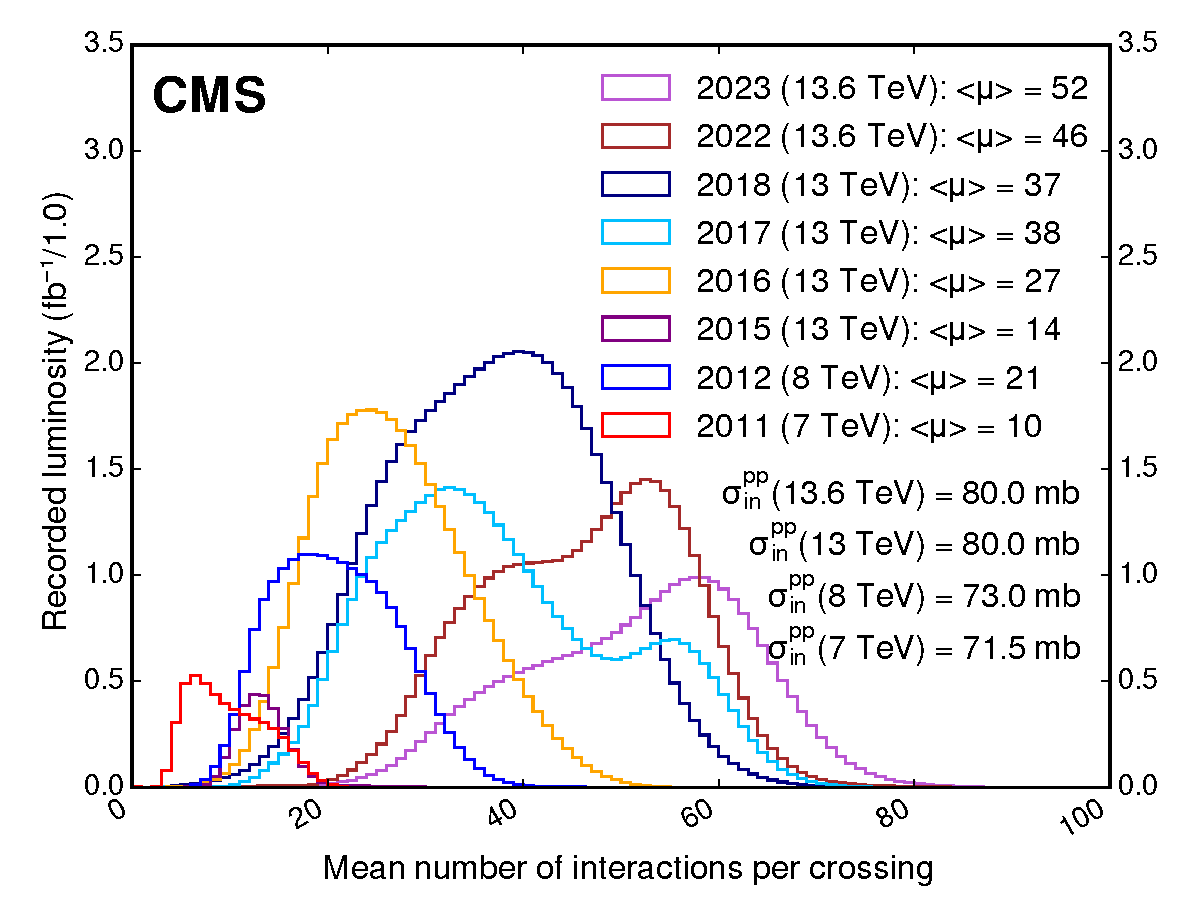
\includegraphics[width=0.8\linewidth]{figs/05_analysis/pileup_allYears.pdf}
	\caption[Pileup distributions and mean PU from 2011-2023 data taking.]{Pileup distributions and mean PU from 2011-2023 data taking~\cite{CMSlumi}.}
	\label{fig:pileup}
\end{figure}

Monte Carlo samples account for secondary collisions by generating PU interactions according to a predetermined distribution. However, the distribution of the number of interactions does not exactly match what is observed in data. To account for this, we apply a weight to simulated samples as a function of the number of simulated PU interactions by dividing a histogram of data PU distributions by the Monte Carlo PU distribution.

\subsubsection{Monte Carlo Background} \label{sec:ana_mcbkg}
Although this analysis employs a data driven method of background estimation, simulated samples are used to inform on properties of background events and tune cuts to discriminate between signal and background. For this analysis, we use simulated Drell-Yan (DY) to $\ell\ell$ events with 0, 1 and 2 additional jets, simulated using matrix elements calculated at NNLO. Studies were done with inclusive (any number of additional jets) samples but found these samples to have worse agreement in control regions and statistical power compared to the jet categorized samples. The cross sections used for normalization were calculated using the \texttt{GenXSecAnalyzer}, a tool provided by CMS to calculate the cross sections for simulated samples~\cite{genxsecana}. A list of cross sections for each simulated process can be found in table~\ref{tab:mcsamples}.

\begin{table}[htb!]
	\centering
	\caption[List of simulated background processes, their cross sections calculated using \texttt{GenXSecAnalyzer}.]
	{List of simulated background processes, their cross sections calculated using \texttt{GenXSecAnalyzer}~\cite{genxsecana}.}
	\label{tab:mcsamples}
	\begin{tabular}{l c}\hline
		Process & Cross Section [pb]\\
		\hline
		DY + 0 jets & 5090 \\
		DY + 1 jet & 983.5\\
		DY + 2 jets & 353.5 \\
		\hline
	\end{tabular}
	
\end{table}

\subsubsection{Scale Factor Corrections} \label{sec:ana_sf}
Scale factors are corrective weights applied to simulated events in order to improve the agreement to data. The total weight applied is defined by the data-to-simulation efficiency ratio, given by
\begin{equation}
	S=\frac{\epsilon(\text{data})}{\epsilon(\text{MC})}
\end{equation}
The total efficiency $\epsilon$ in data and Monte Carlo is a product of the efficiencies for each object used in the event selection. The efficiency for a given object is itself a product of several individual efficiencies. For muons, the efficiency $\epsilon_\PGm=\epsilon_\text{reco}\times\epsilon_\text{trig}\times\epsilon_\text{ID}\times\epsilon_\text{iso}$ is a product of the muon track reconstruction efficiency, trigger efficiency, ID efficiency, and isolation efficiency. For electrons and photons, $\epsilon_\text{iso}$ is absorbed into the $\epsilon_\text{ID}$ efficiency because the cut based ID includes the isolation. The efficiency for electrons is then $\epsilon_e=\epsilon_\text{reco}\times\epsilon_\text{trig}\times\epsilon_\text{ID}$. Photons are not used for any HLT triggers nor do they have associated tracks, so $\epsilon_\text{trig}$ and $\epsilon_\text{reco}$ are omitted, making the total efficiency $\epsilon_\gamma=\epsilon_\text{pix}\times\epsilon_\text{ID}$, where $\epsilon_\text{pix}$ is the efficiency for the pixel seed veto. The total scale factor is then given by
\begin{equation}
	S=\prod_{i\in\PGm,e,\gamma}\frac{\epsilon_i(\text{data})}{\epsilon_i(\text{MC})}
\end{equation}
All scale factors are centrally measured and provided by the respective POGs with the exception of the electron trigger efficiencies, which were privately produced. Almost all efficiencies are measured with the tag-and-probe technique, which uses events containing one lepton passing strict selection criteria (the ``tag '') and one oppositely charged same flavor lepton passing loose selection criteria (the ``probe ''), where the dilepton invariant mass lies within the \PZ resonance centered at $91\GeV$. The strict tag and invariant mass criteria give a set of real leptons that are unbiased due to the loose probe criteria which are used to calculate various efficiencies. This method was adapted for photon ID efficiency calculations by ignoring the tracker information for $\PZ\to\Pe\Pe$ events and treating the calorimeter clusters as photons. The photon pixel seed veto efficiencies require tracker information and cannot be calculated using $\PZ\to\Pe\Pe$ tag-and-probe techniques. These were instead measured using $\PZ\to\PGm\PGm+\gamma$ events, where the photon is from final state radiation. Invariant mass and topological cuts give a clean sample of unbiased photons which are used to calculate $\epsilon_\text{pix}$.

Electron HLT scale factors were not centrally provided and were calculated privately using the tag-and-probe technique described above. The tag-and-probe were required to have a combined invariant mass of $60<m_\text{tag-probe}<125\GeV$. Baseline criteria for the tag and probe can be seen in table~\ref{tab:tnp}.
\begin{table} [htb!]
	\centering
	\caption{Tag and probe criteria used to derive HLT scale factors}
	\label{tab:tnp}
	\begin{tabular}{l | l}
		\hline
		Tag Criteria & Probe Criteria \\
		\hline
		\hline
		\begin{tabular}{l}
			Matched to Single Electron Trigger\\
			Passing tight cut-based ID\\
			$|\eta| < 2.17$\\
			$|\eta| < 1.4442$ or $|\eta| > 1.566$\\
			$\pt > 35\GeV$\\
		\end{tabular}  & 
		\begin{tabular}{l}
			$\pt > 15\GeV$\\
			$|\eta| < 2.5$\\
			$E_{T} > 5\GeV$\\
			$|d_{z}| < 0.2\unit{cm}$ \\
			$|d_{xy}| < 0.2\unit{cm}$\\
			Passes tight cut-based ID\\
		\end{tabular} \\
		\hline
	\end{tabular}
\end{table}

Events that pass the baseline tag/probe criteria are binned according to the \pt and $\eta_{sc}$ of the probe, and split into pass/fail histograms if the probe passed/failed to trigger the HLT path. For data, the histograms are fit analytically using the \PZ peak plus background to extract the number of signal events and calculate the efficiency. In Monte Carlo, the events are first matched to generator level electrons originating from the \PZ to ensure zero background events and fit to only the \PZ signal. The signal is modeled using a piecewise function with the upper and lower sides modeled using gaussian cores and exponential tails, which is then convolved with the world-average \PZ mass and width~\cite{Sirunyan_2021}. Background is modeled by multiplying an error function with a falling exponential. To calculate the systematic uncertainty of the fit, the efficiencies are calculated for data under alternative signal and background models. For the alternate signal, the data models the signal shape as a convolution of a gaussian and the Monte Carlo signal from the equivalent bin. For the alternate background, the shape is modeled as just an exponential, which can either grow or decay depending on the \pt and $\eta$ range of the bin. This process is repeated for each era, as the trigger and run conditions can vary between years. The trigger efficiency as a function of $\eta$ can be seen in figure~\ref{fig:effVsEta_electronHLT}. A full set of scale factors is shown in figures~\ref{fig:UL2018_SF2D} - \ref{fig:UL2016_preVFP_SF2D}.

\begin{figure}[htb!]
	\centering
	\captionsetup[subfigure]{justification=centering}
	\begin{subfigure}[h]{0.45\linewidth}
		\centering
		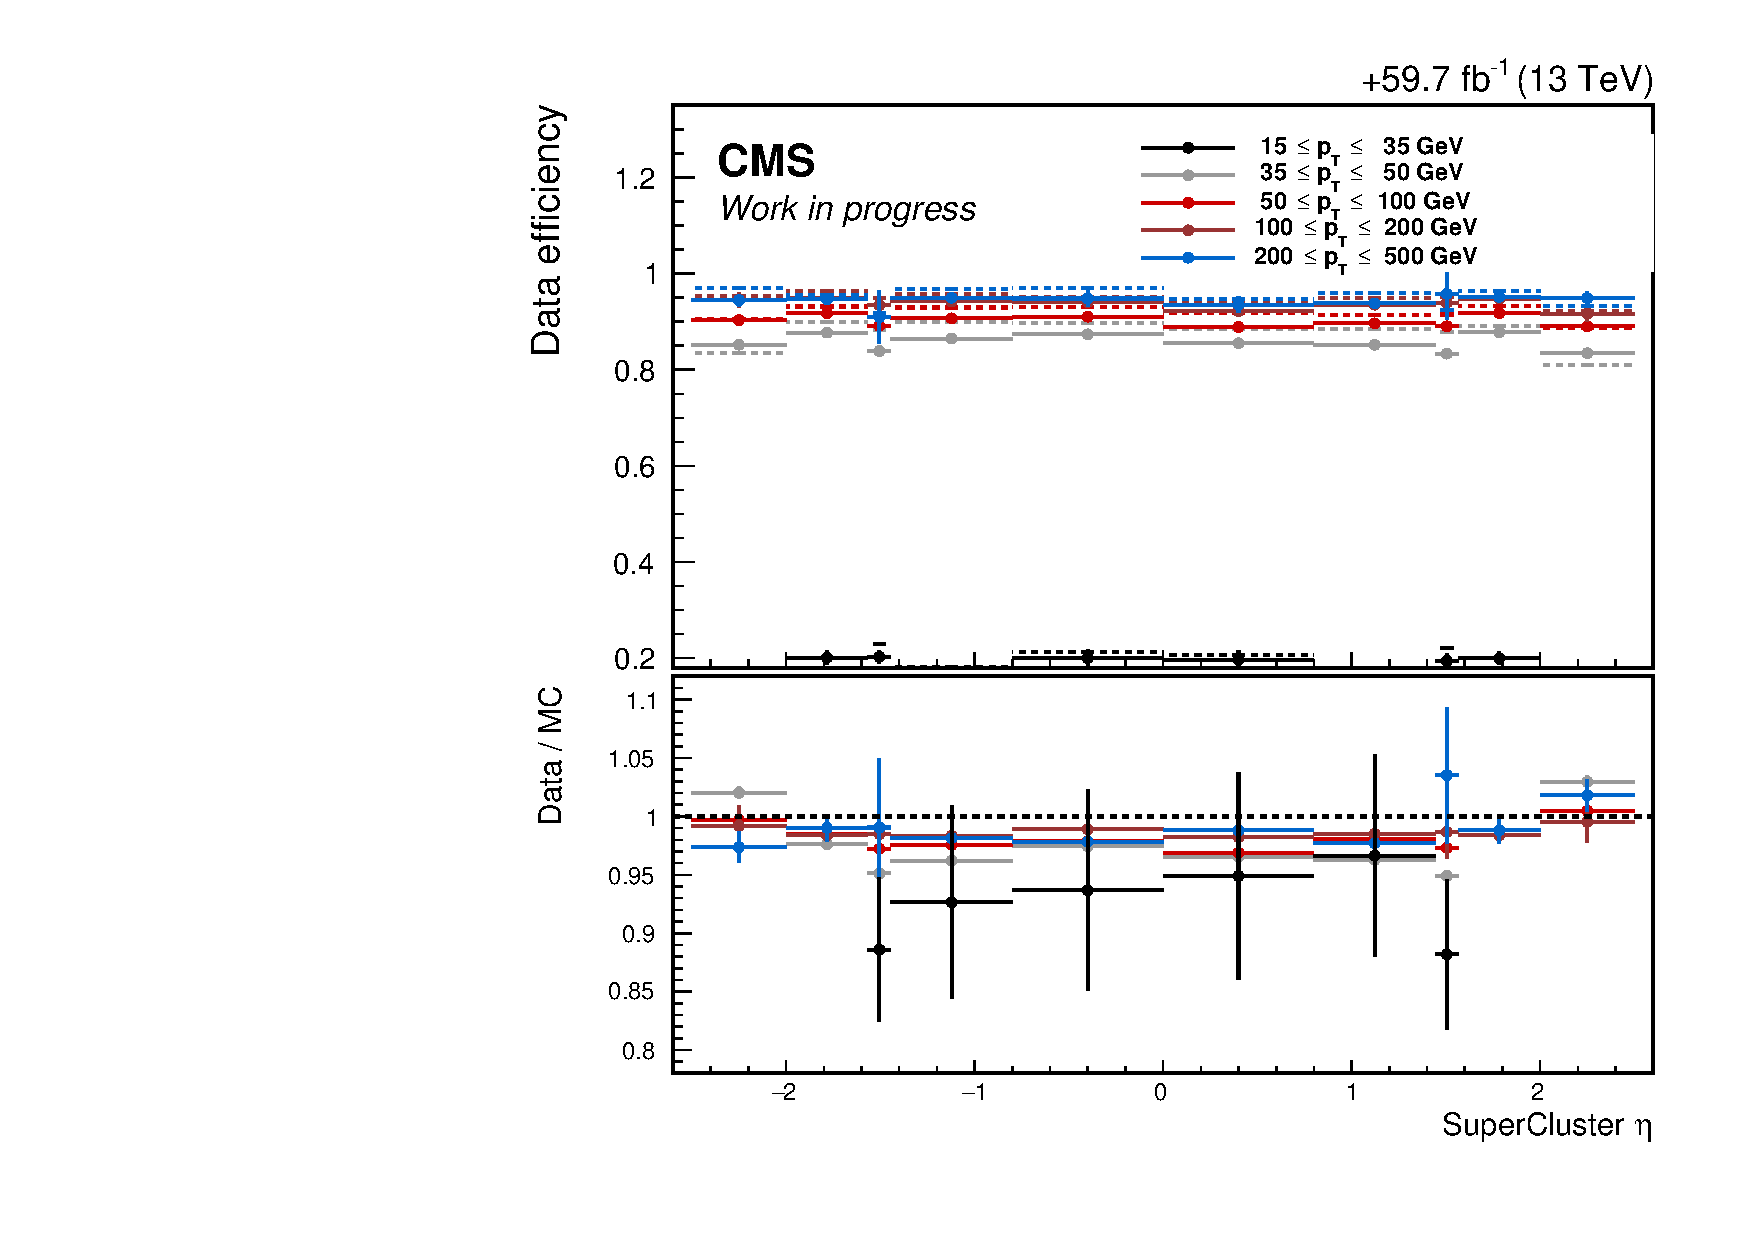
\includegraphics[width=\linewidth]{figs/05_analysis/UL2018_SFvseta_myWP.pdf}
		\caption{2018}
	\end{subfigure}
	\begin{subfigure}[h]{0.45\linewidth}
		\centering
		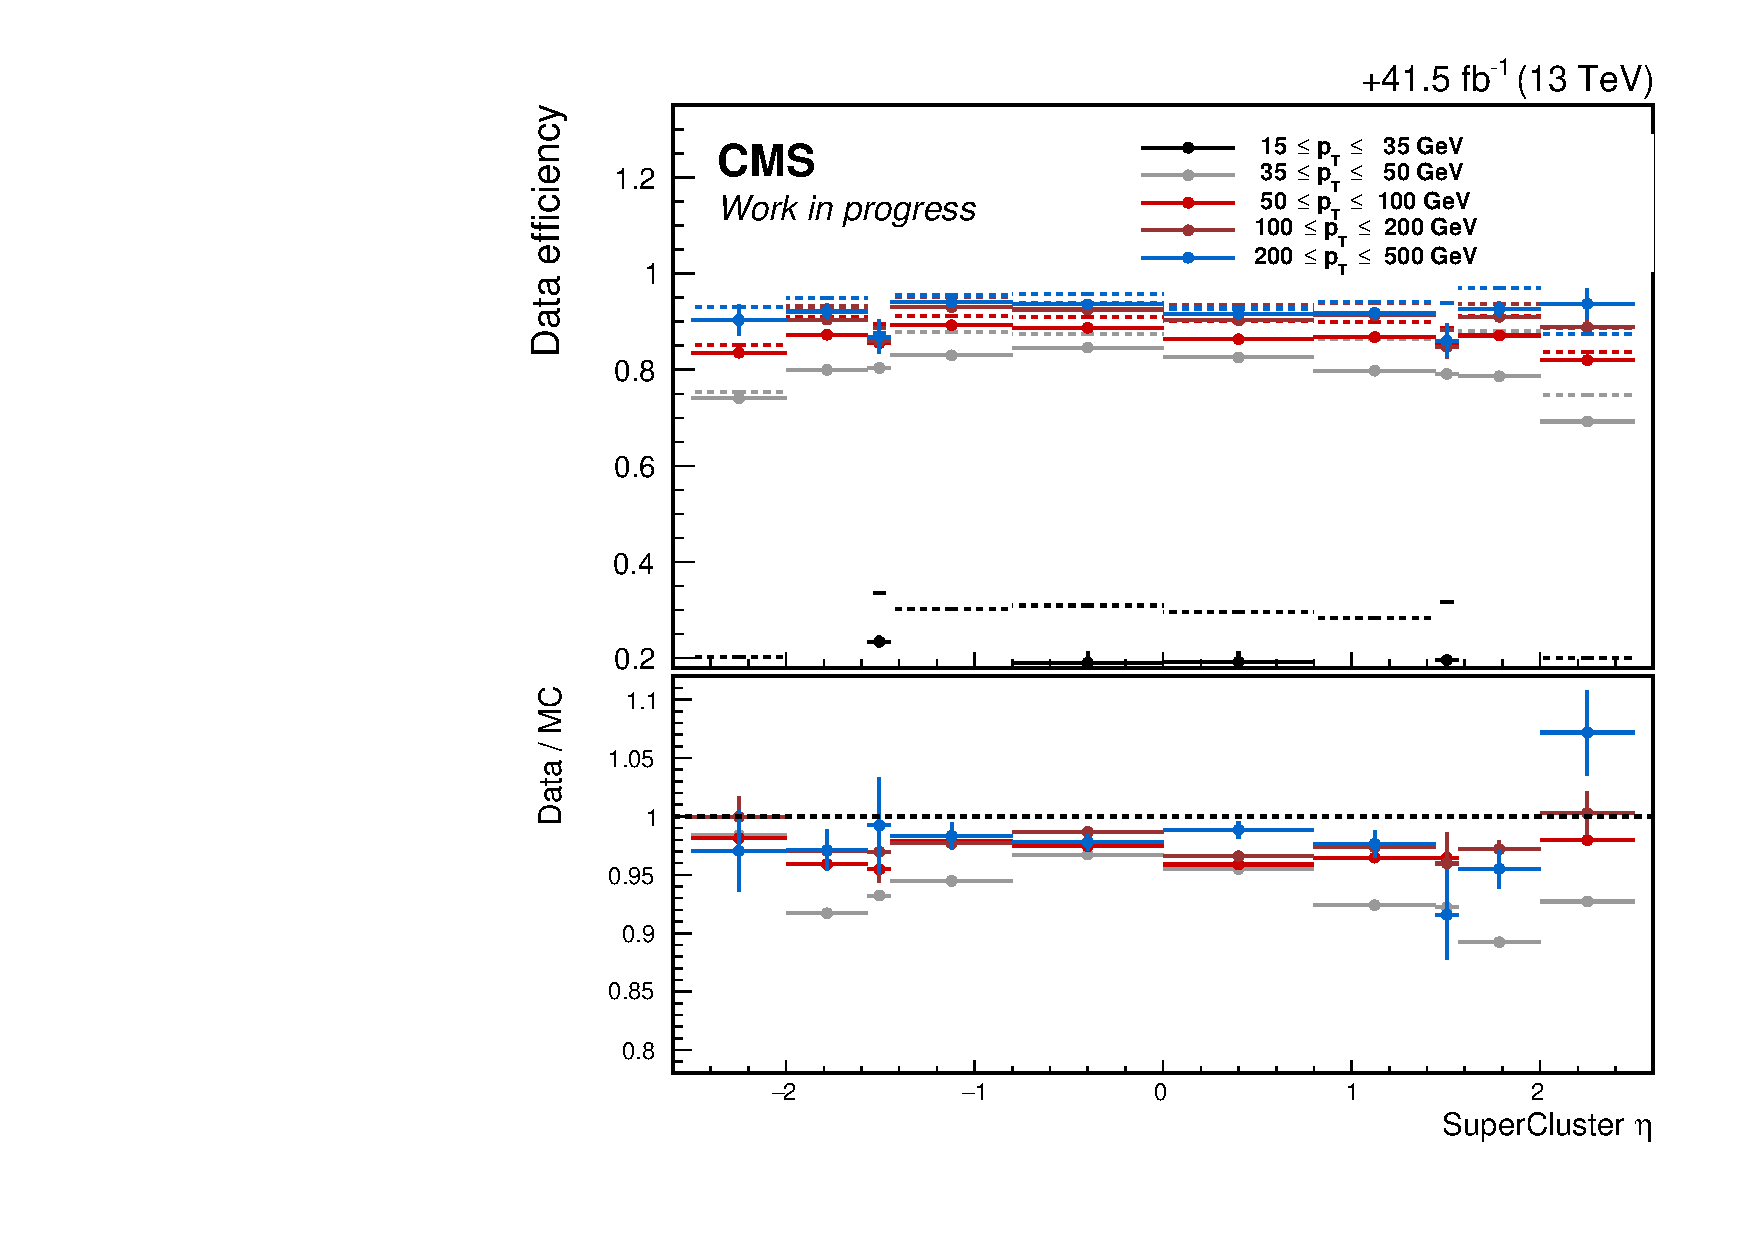
\includegraphics[width=\linewidth]{figs/05_analysis/UL2017_SFvseta_myWP.pdf}
		\caption{2017}
	\end{subfigure}
	\begin{subfigure}[h]{0.45\linewidth}
		\centering
		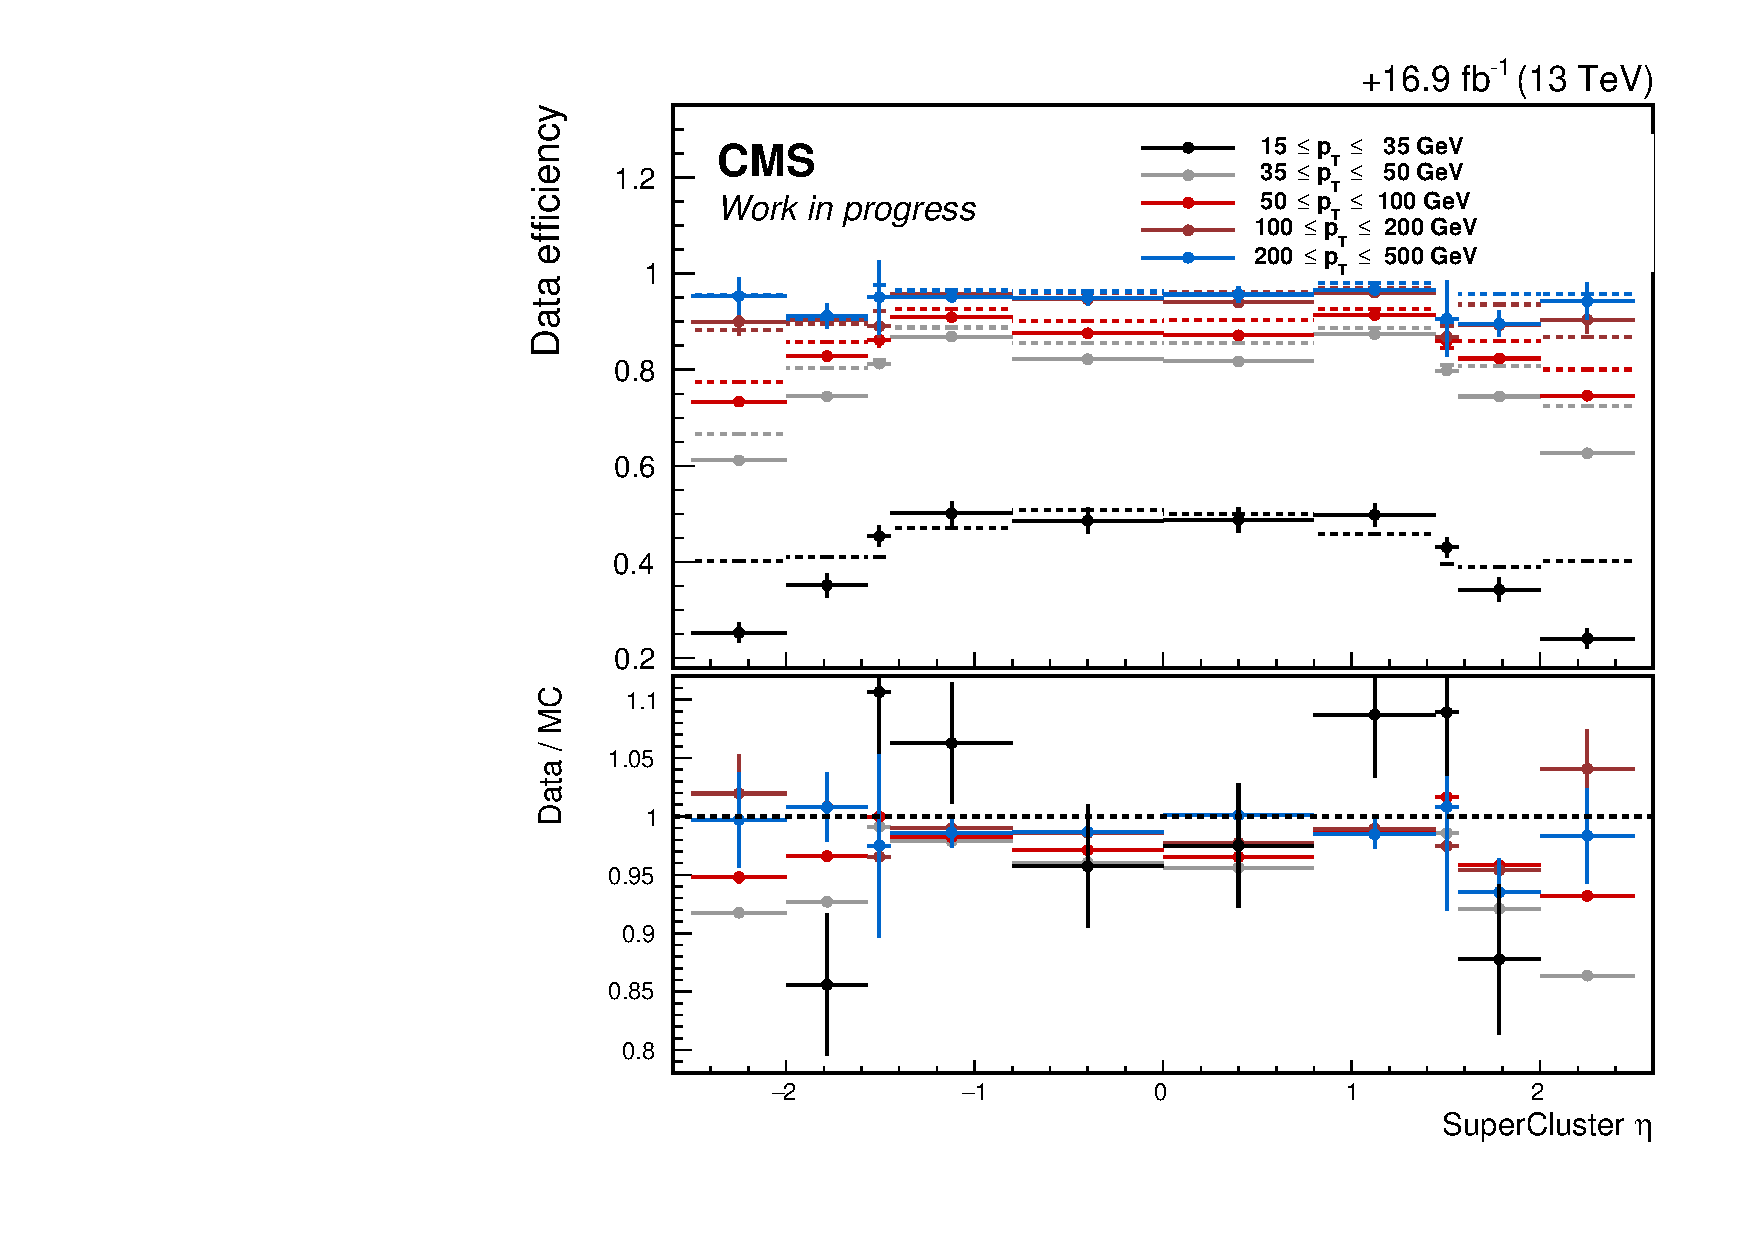
\includegraphics[width=\linewidth]{figs/05_analysis/UL2016_postVFP_SFvseta_myWP.pdf}
		\caption{2016 post-VFP}
	\end{subfigure}
	\begin{subfigure}[h]{0.45\linewidth}
		\centering
		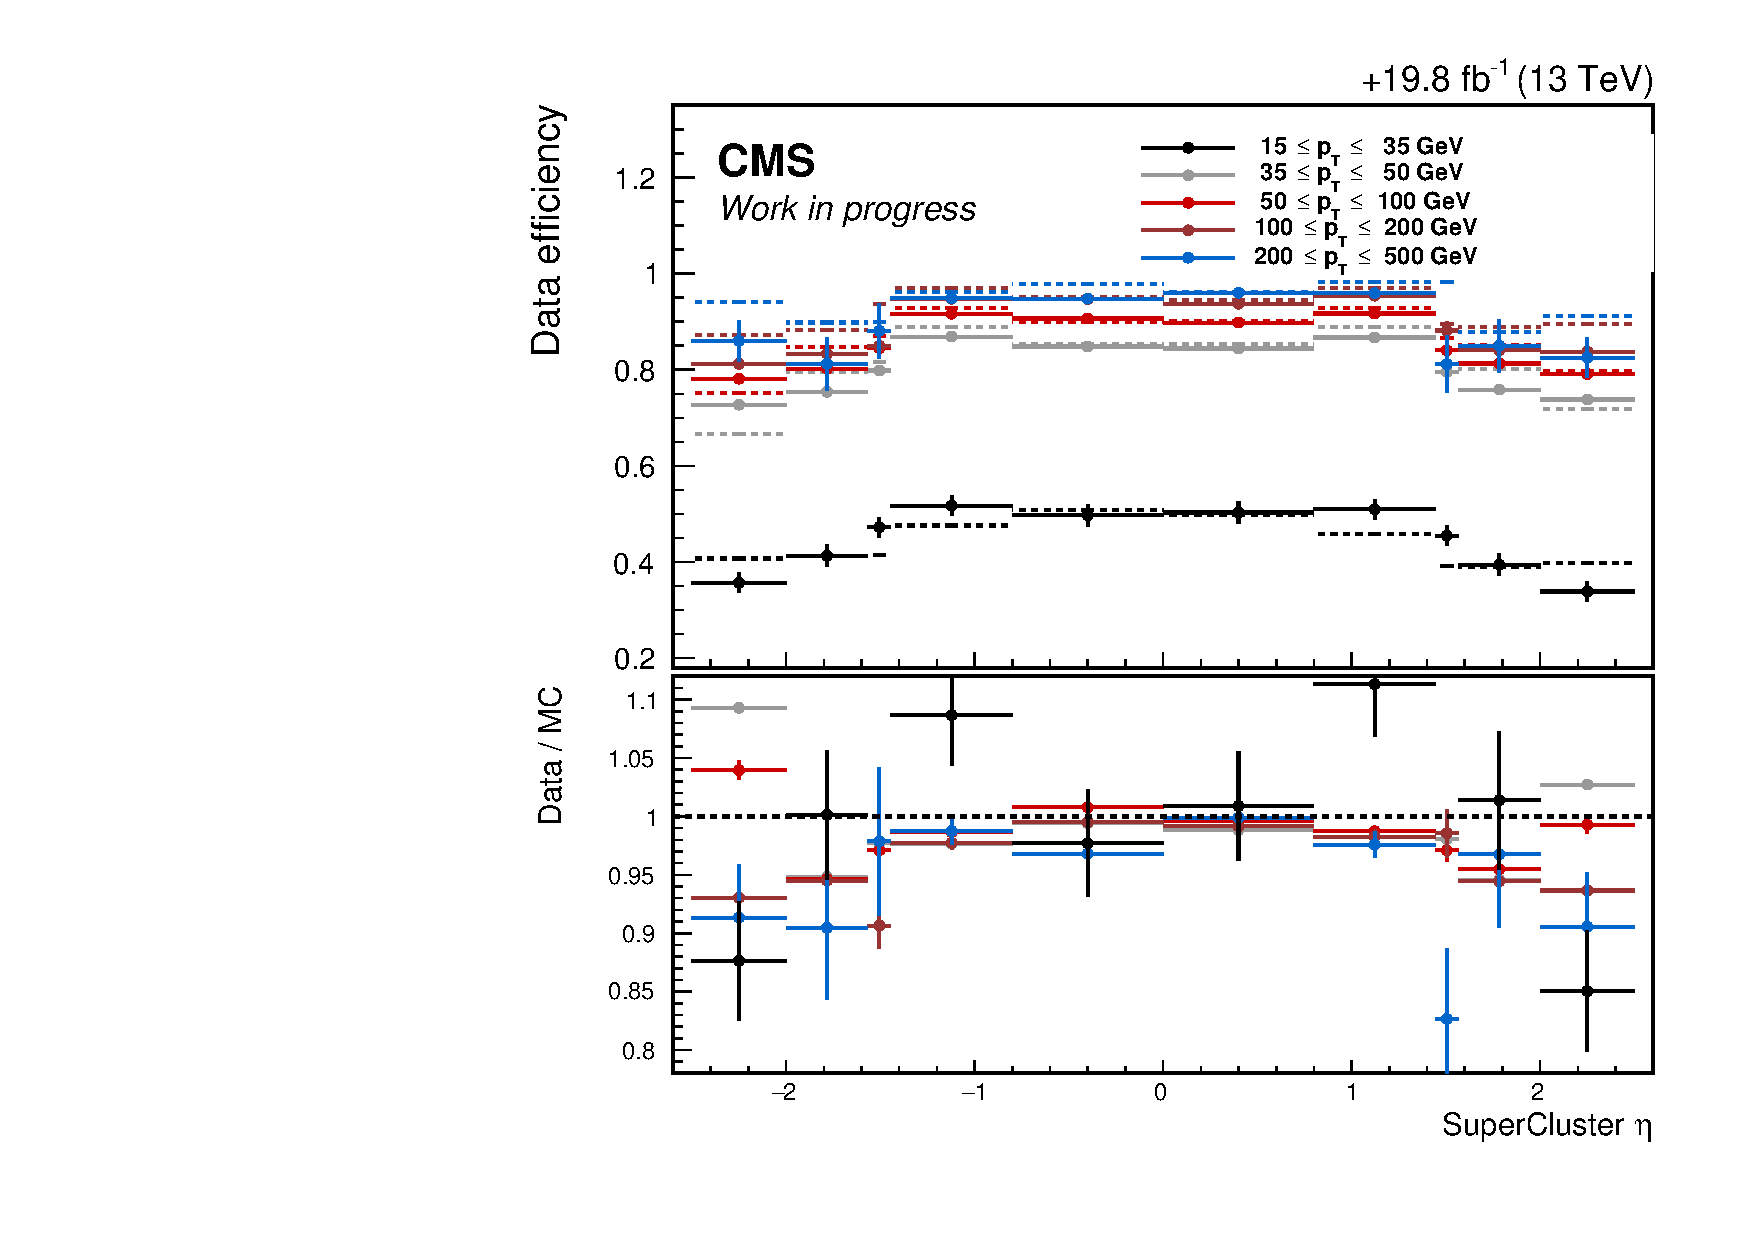
\includegraphics[width=\linewidth]{figs/05_analysis/UL2016_preVFP_SFvseta_myWP.pdf}
		\caption{2016 pre-VFP}
	\end{subfigure}
	\caption[Trigger efficiency as a function of $\eta_{sc}$ for several ranges of electron $\pt$ for all data taking eras.]{Trigger efficiency as a function of $\eta_{sc}$ for several ranges of electron $\pt$ for all data taking eras.}
	\label{fig:effVsEta_electronHLT}
\end{figure}

\begin{figure}[htb!]
	\centering
	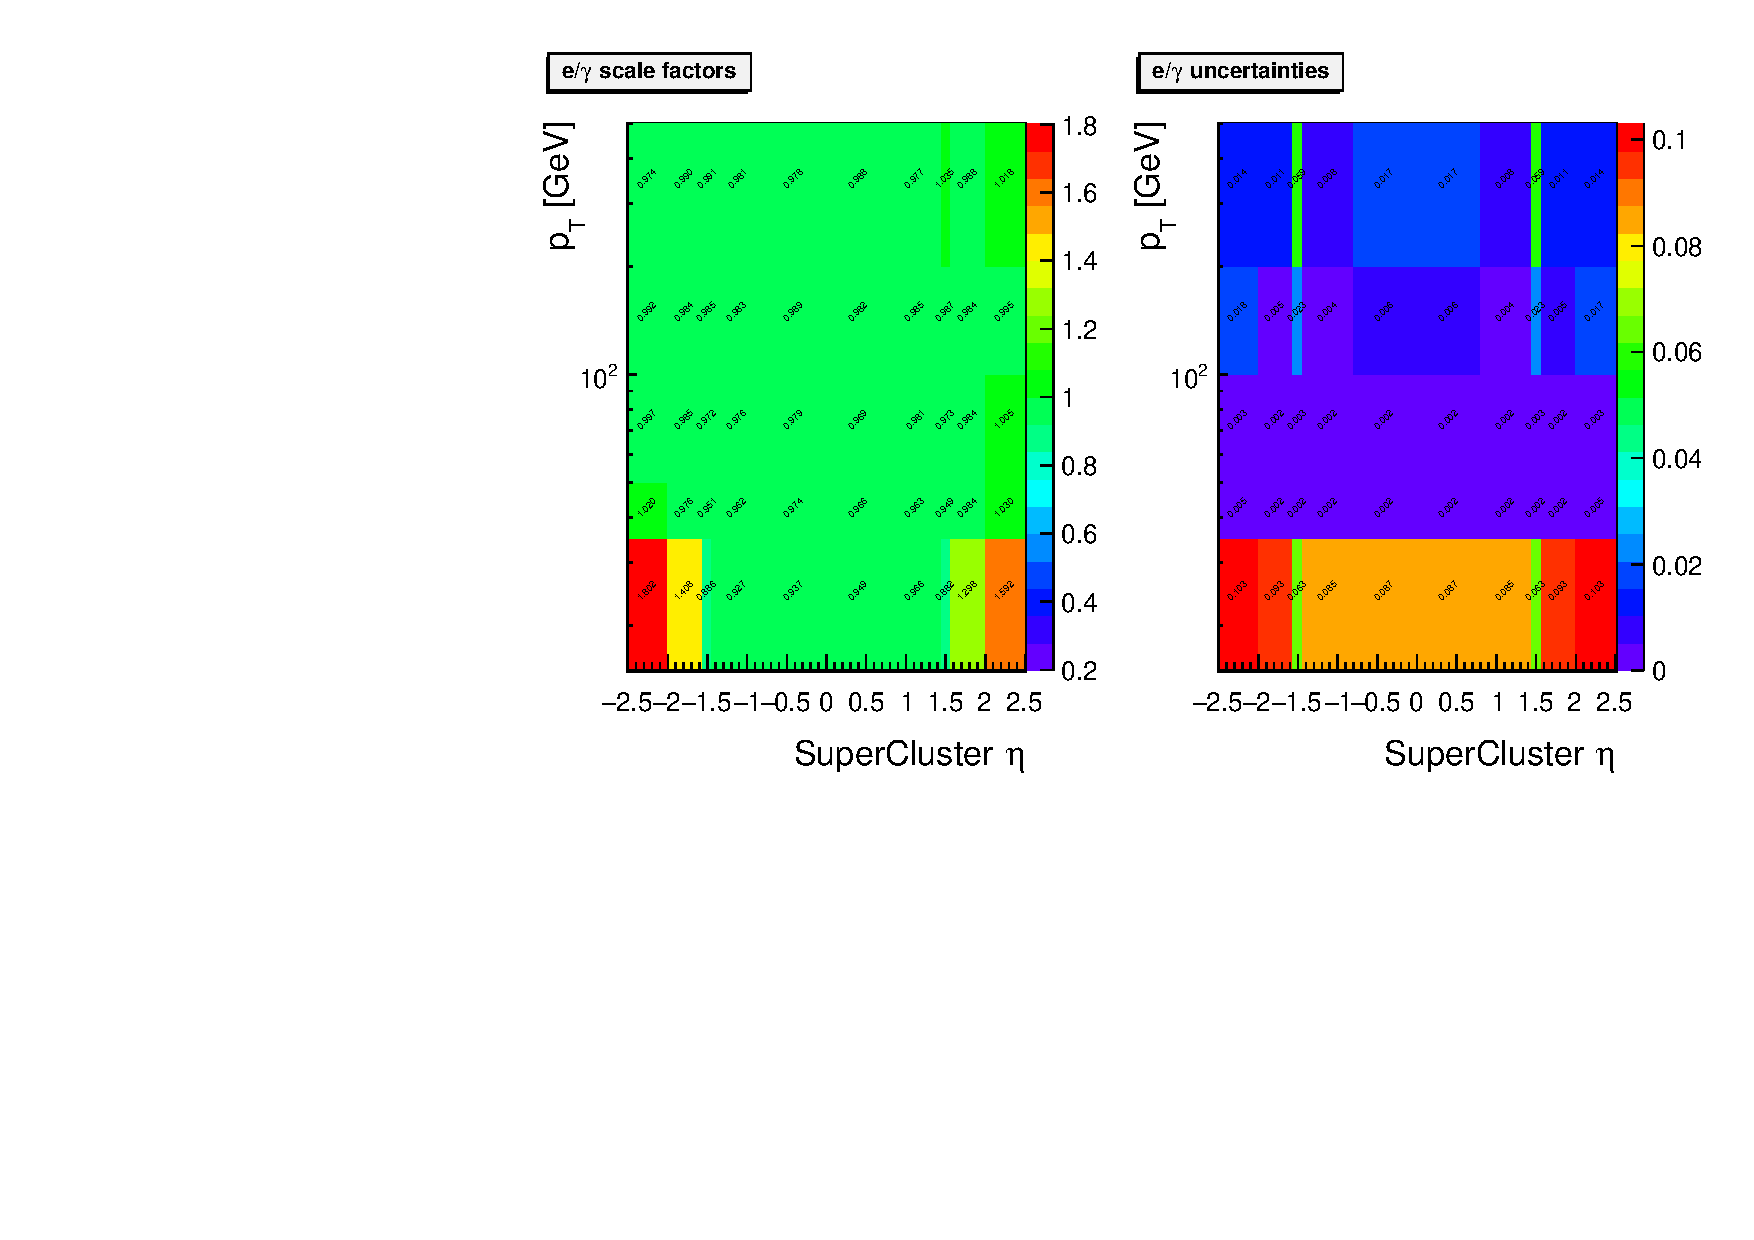
\includegraphics[width=0.85\linewidth]{figs/05_analysis/UL2018_SF2D_myWP.pdf}
	\caption[2018 electron HLT scale factors and uncertainties.]{2018 electron HLT scale factors and uncertainties.}
	\label{fig:UL2018_SF2D}
\end{figure}

\begin{figure}[htb!]
	\centering
	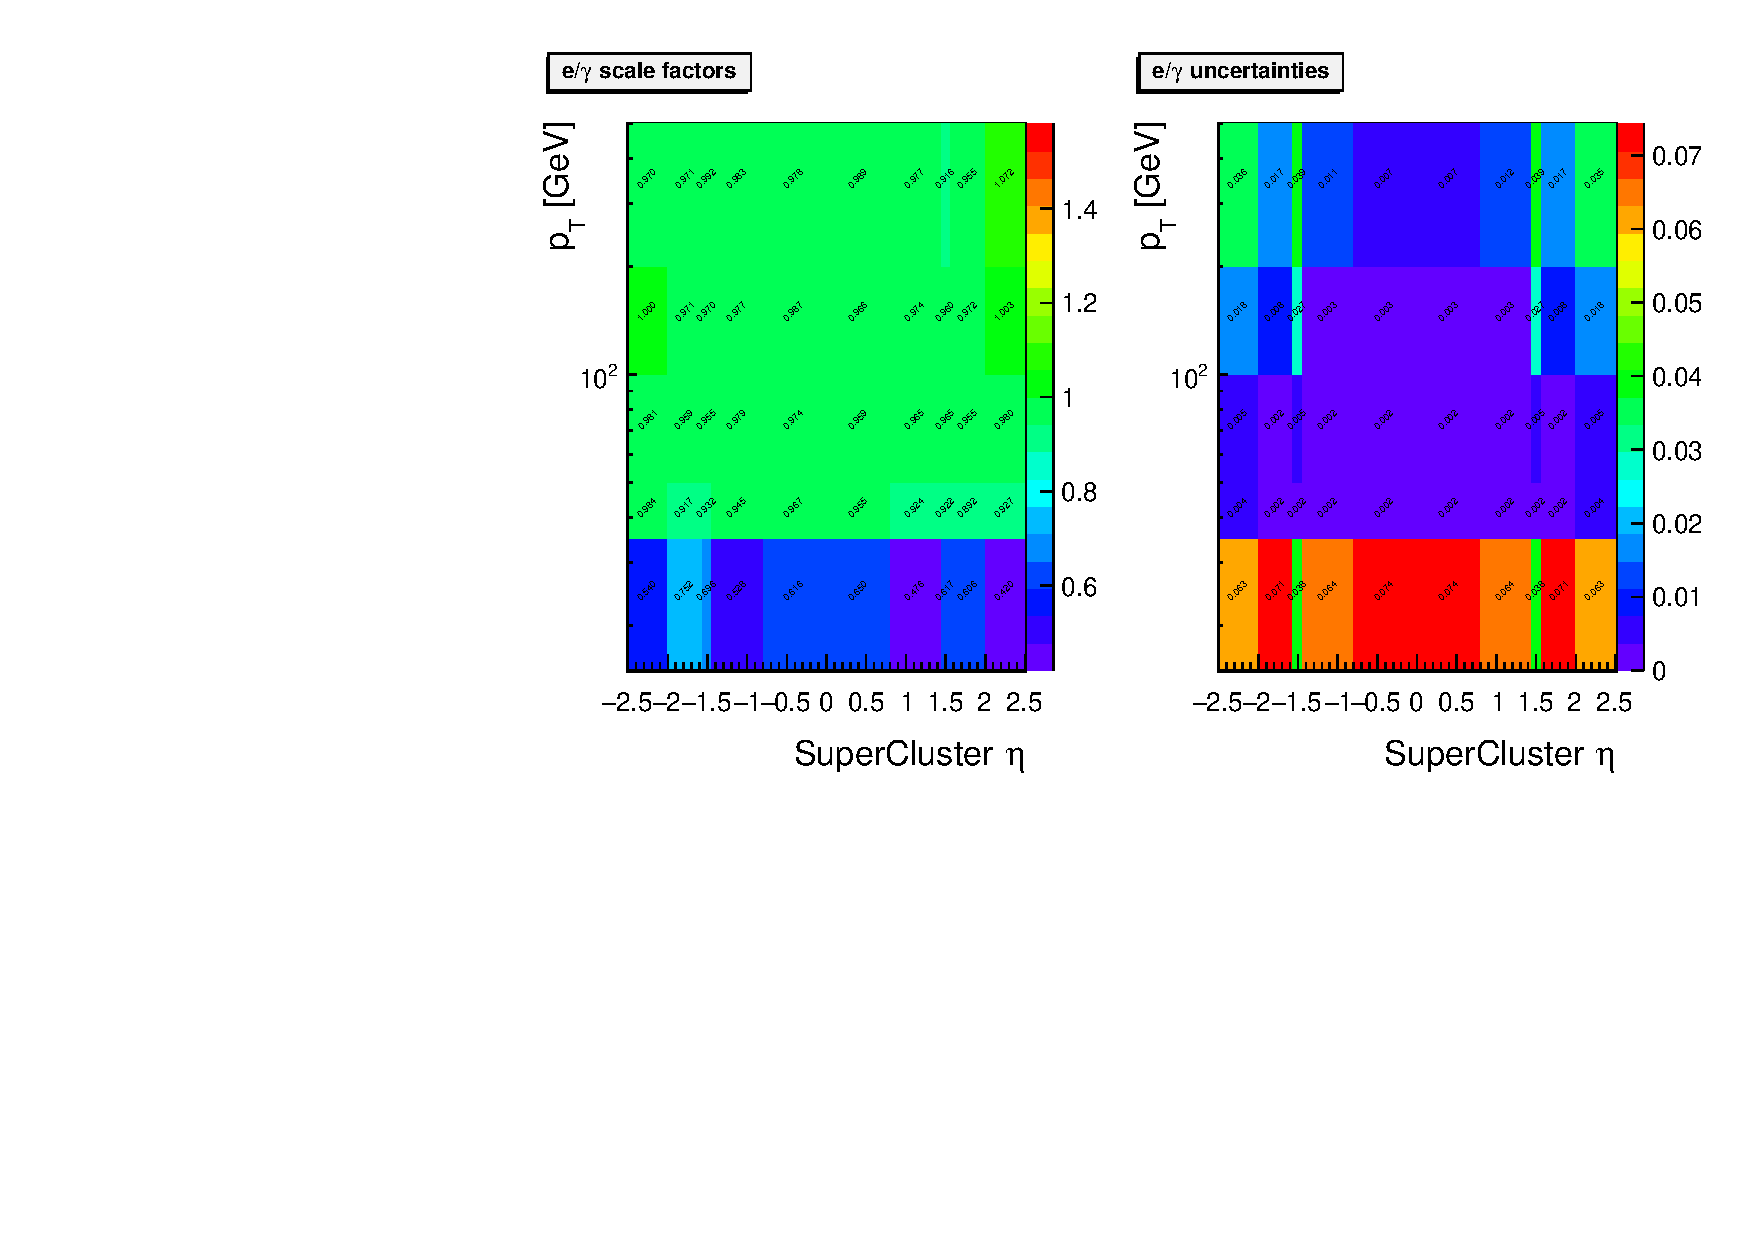
\includegraphics[width=0.85\linewidth]{figs/05_analysis/UL2017_SF2D_myWP.pdf}
	\caption[2017 electron HLT scale factors and uncertainties.]{2017 electron HLT scale factors and uncertainties.}
	\label{fig:UL2017_SF2D}
\end{figure}

\begin{figure}[htb!]
	\centering
	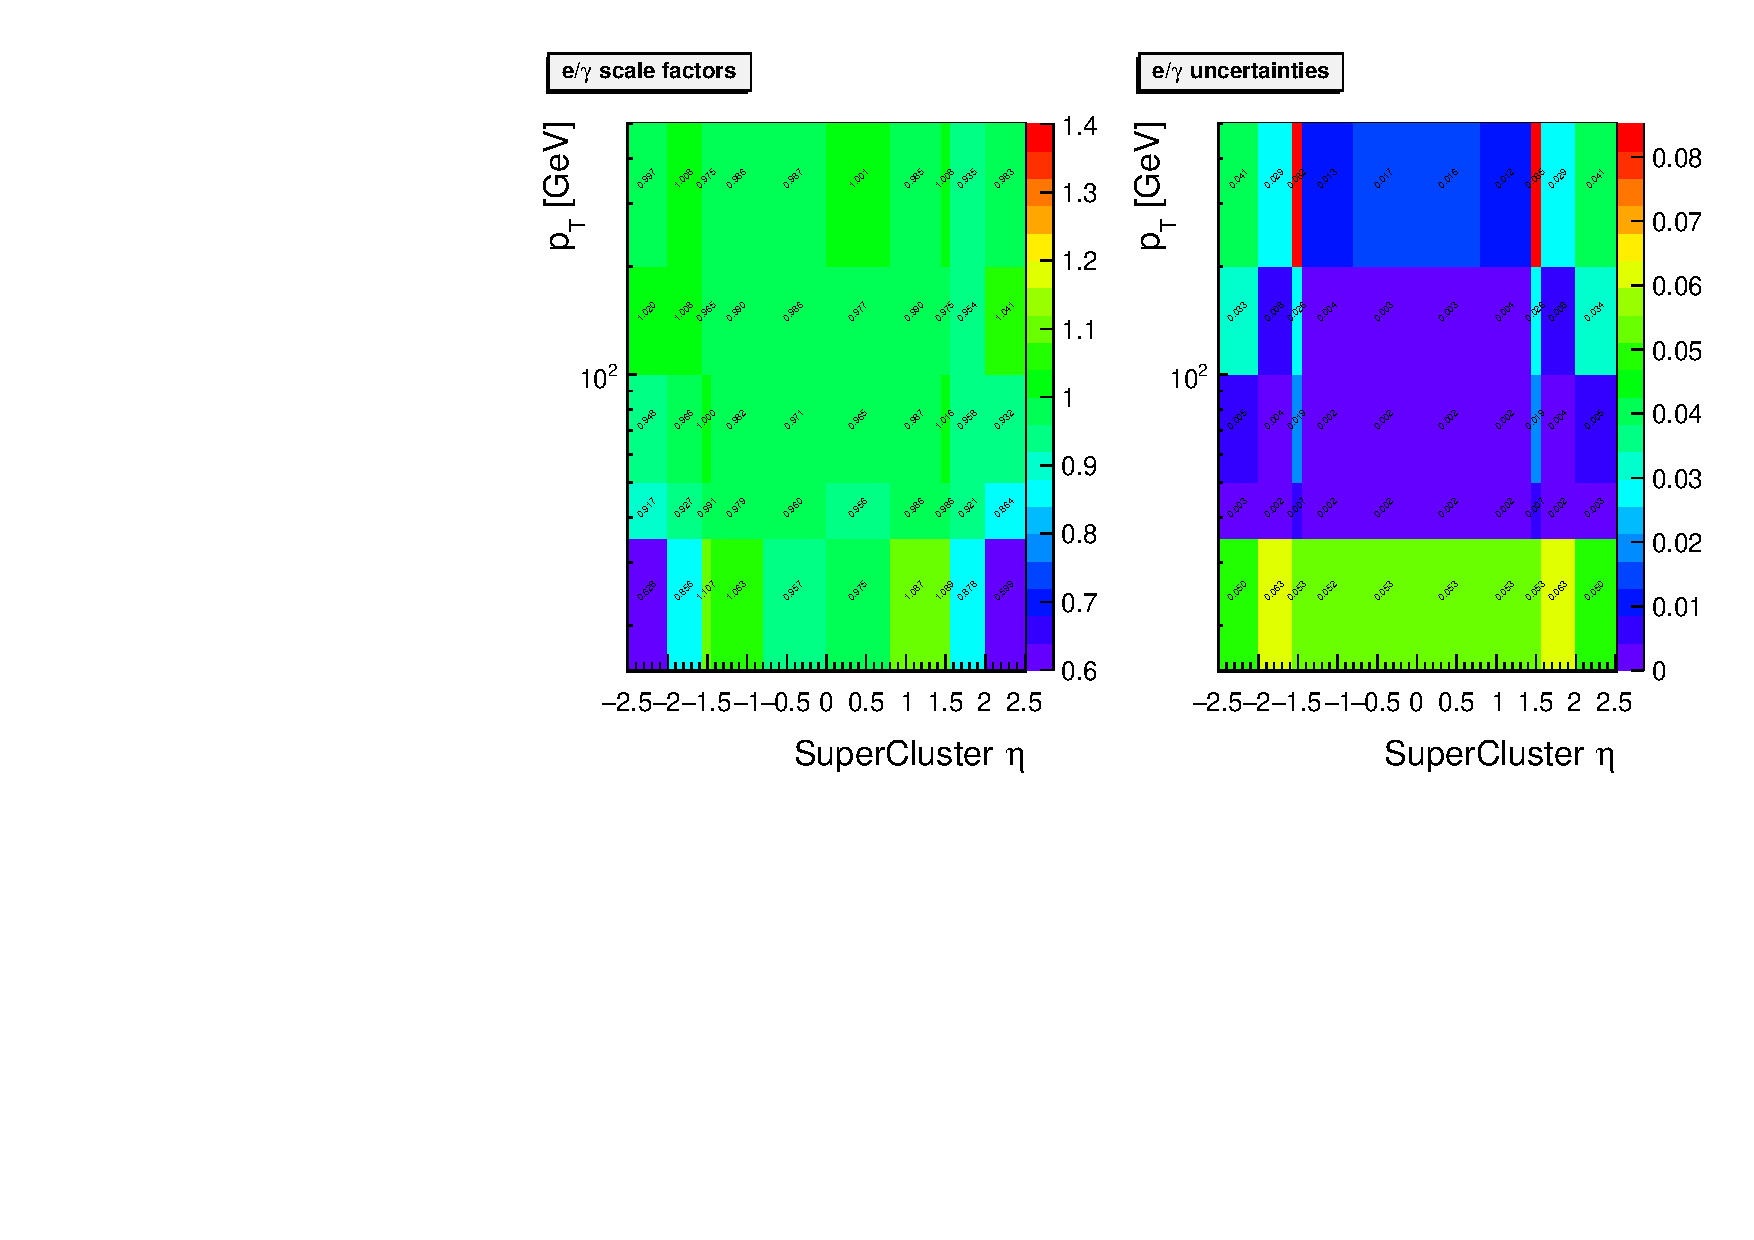
\includegraphics[width=0.85\linewidth]{figs/05_analysis/UL2016_postVFP_SF2D_myWP.pdf}
	\caption[2016 post-VFP electron HLT scale factors and uncertainties.]{2016 post-VFP electron HLT scale factors and uncertainties.}
	\label{fig:UL2016_postVFP_SF2D}
\end{figure}

\begin{figure}[htb!]
	\centering
	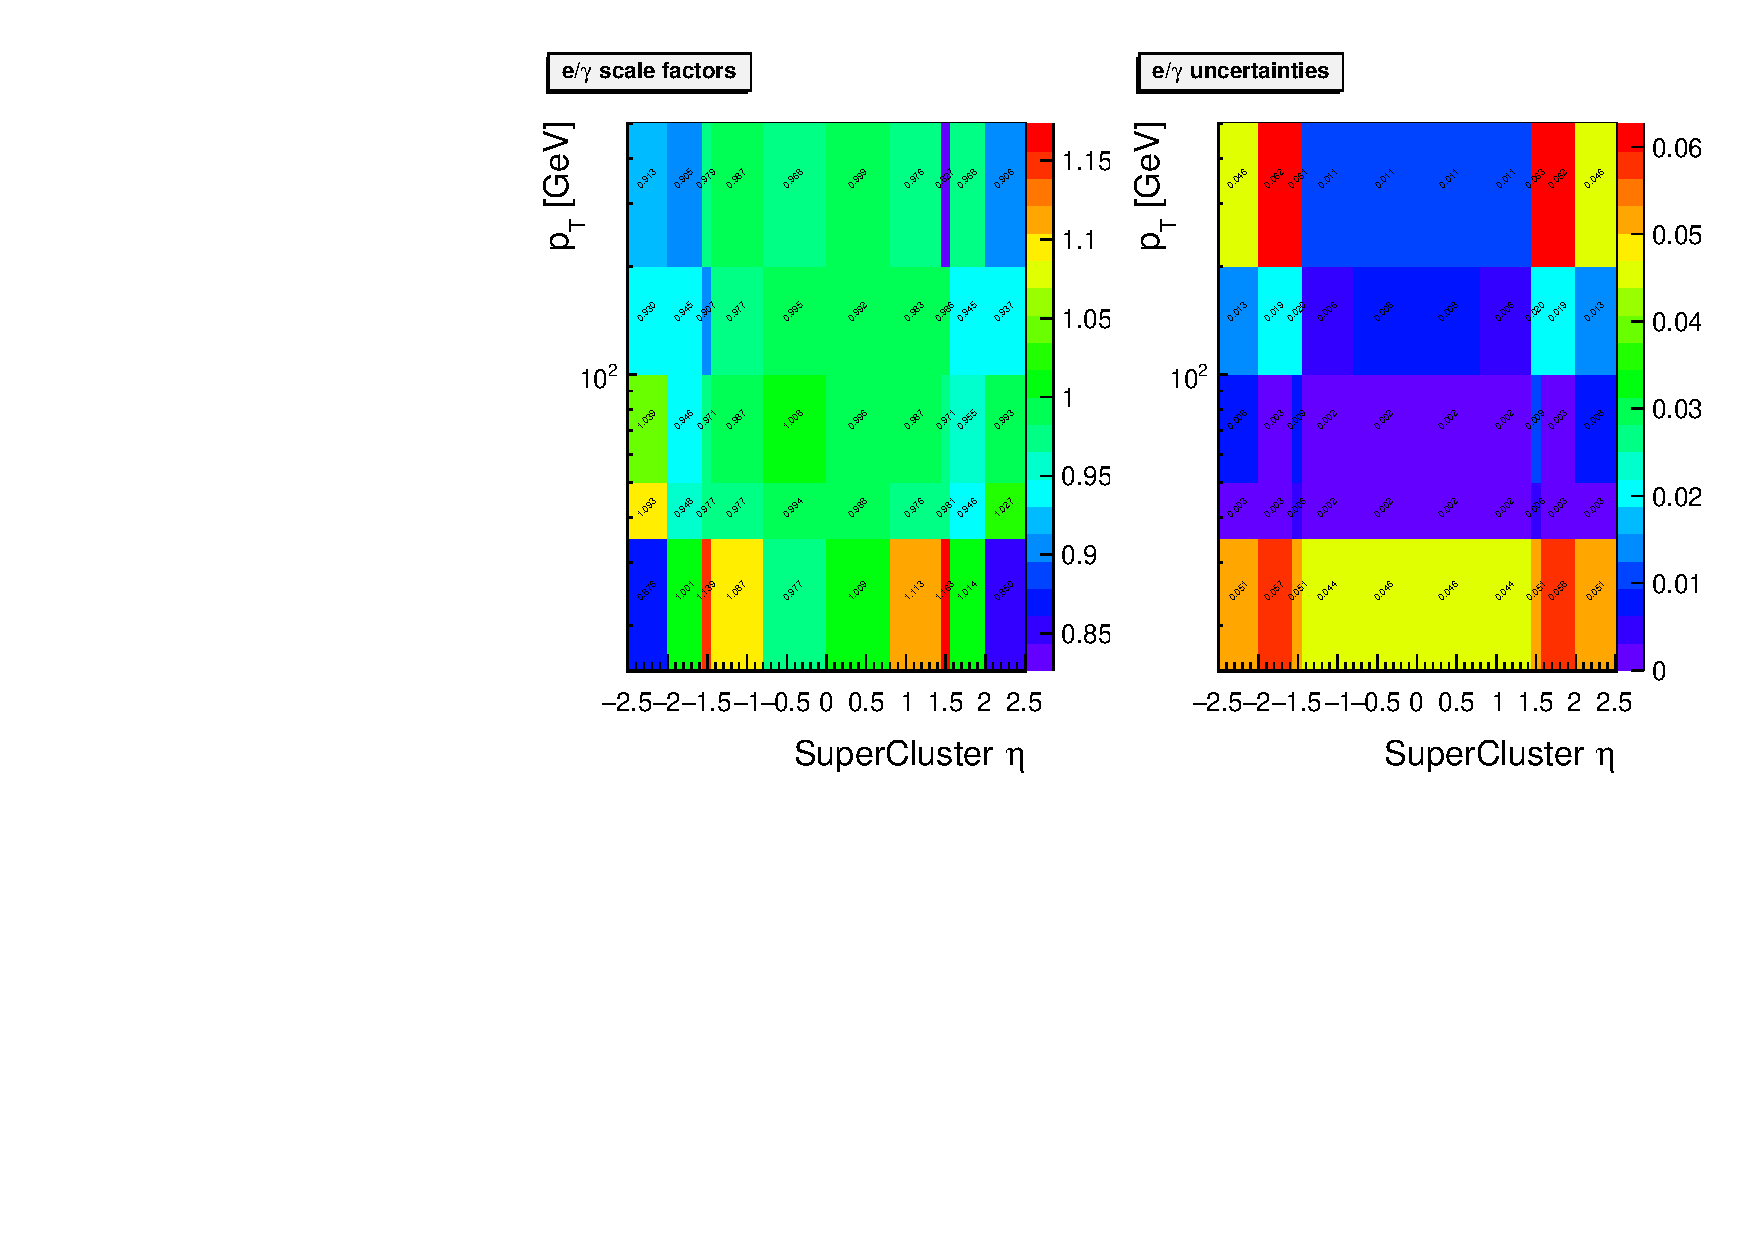
\includegraphics[width=0.85\linewidth]{figs/05_analysis/UL2016_preVFP_SF2D_myWP.pdf}
	\caption[2016 pre-VFP electron HLT scale factors and uncertainties.]{2016 pre-VFP electron HLT scale factors and uncertainties.}
	\label{fig:UL2016_preVFP_SF2D}
\end{figure}

Muon reconstruction, isolation, and ID scale factors are applied for each muon used to reconstruct the \PZ as a function of $\pt$ and $|\eta|$. Muon trigger scale factors are as a function of $\pt$, $\eta$ and charge of the triggering muon, or the higher \pt muon if both pass the single muon trigger. The photon ID and all electron scale factors are applied as a function of electron \pt and $\eta$, with the electron HLT scale factor application following the same logic as the muon HLT. Lastly, the photon pixel seed veto scale factor is applied as a function of the $\eta$ region (barrel or endcap) of the photons. Most scale factors are on the order of a few percent with uncertainties less than 0.1\%.


\section{Vertex Reconstruction of Displaced Photon Pairs} \label{sec:ana_vertex}
\subsection{Diphoton Kinematics} \label{sec:vertex_calc}
The kinematics of a long lived, massive scalar boson $\Phi$ decaying to two photons can be precisely described by the following
\begin{equation}\label{eq:me1e2theta}
	\text{m}_{\Phi}^2 = 2\text{E}_1\text{E}_2(1-\cos\theta)
\end{equation}
where the m$_\Phi$ is the mass of the $\Phi$, E$_1$ and E$_2$ are the energies of the two photons, and $\theta$ is the angle between the two photons. The energy of the two photons is measured by the CMS ECAL, thus $\theta$ can be calculated as a function of m$_\Phi$. Due to the primary vertex, decay vertex, and ECAL clusters being coplanar, this calculation is treated as a 2 dimensional problem. It is a trivial procedure to rotate the system to calculate the vertex, then rotate back to detector coordinates once the decay vertex is calculated. Let the position of the two ECAL clusters be \textbf{r$_1$} and \textbf{r$_2$}. The system can be rotated by an angle
\begin{equation} \label{eq:rot_angle}
	\varphi=\arccos\left(\frac{\textbf{r}_1\times\textbf{r}_2}{\|\textbf{r}_1\times\textbf{r}_2\|}\cdot\hat{z}\right)
\end{equation}
around an axis given by 
\begin{equation} \label{eq:rot_axis}
	\hat{n}=\frac{\textbf{r}_1\times\textbf{r}_2}{\|\textbf{r}_1\times\textbf{r}_2\|}\times\hat{z}
\end{equation}
to determine the decay vertex, then rotated by $-\varphi$ around the same axis to give the final value.

The geometry of the vertex fit is described in figure~\ref{fig:vertex_diagram}. Assume we have two ECAL clusters and a given value of m$_\Phi$. This fixes the value of $\theta$ from equation~\ref{eq:me1e2theta}. It will be shown that the locus of points satisfying these constraints corresponds to the arcs of two circles that overlap the ECAL clusters.

\begin{figure}[htb]
	\centering
	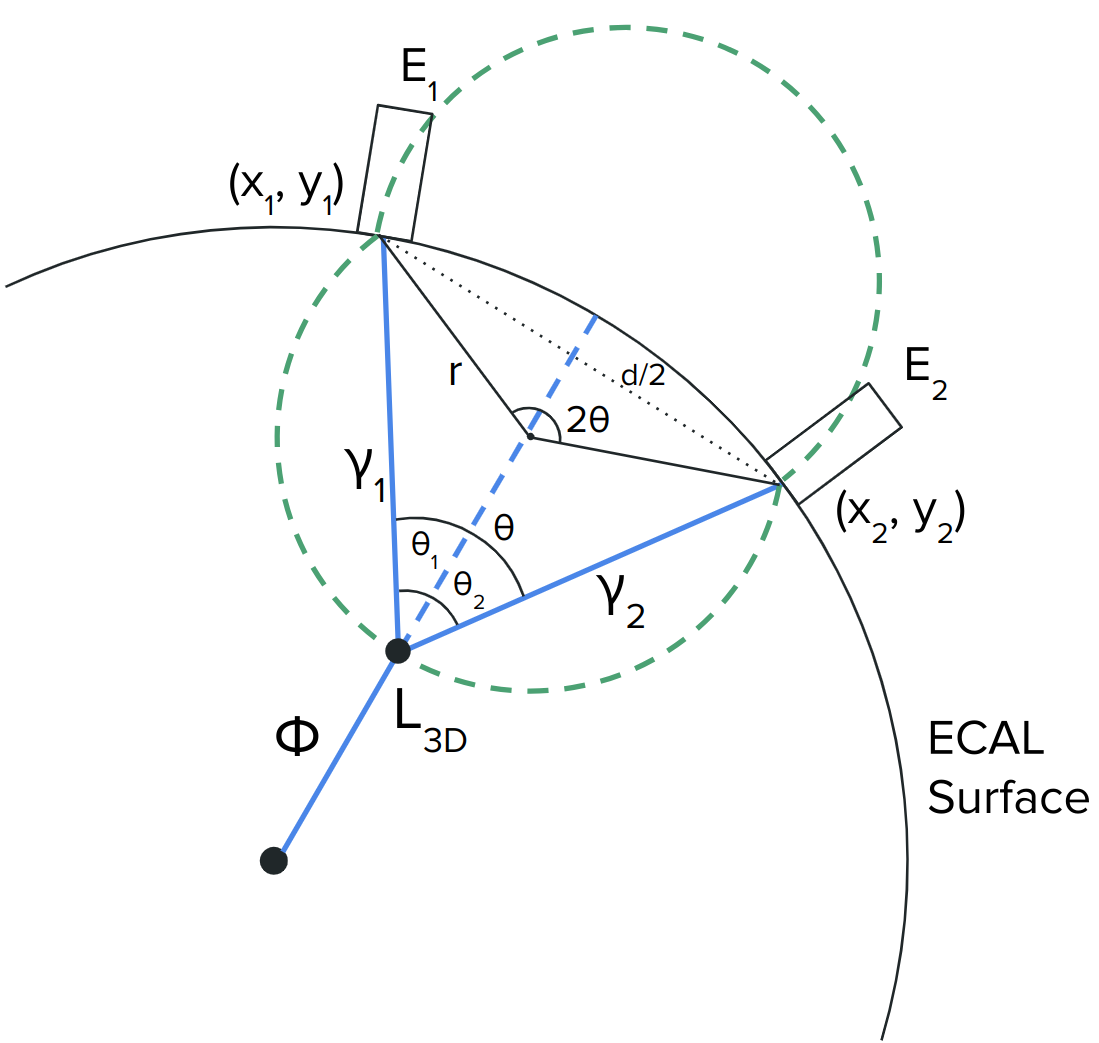
\includegraphics[width=0.65\linewidth]{figs/05_analysis/vertexfit_diagram.png}
	\caption{Geometrical configuration used to reconstruct the displaced vertex of the di-photon pair}
	\label{fig:vertex_diagram}
\end{figure}

Because three non-colinear points uniquely define a circle, $\theta$ corresponds to an inscribed angle on a circle which overlaps the decay vertex and the two ECAL clusters located at $(x_1, y_1)$ and $(x_2, y_2)$. The central angle of the arc between the two clusters has measure $2\theta$ by the inscribed angle theorem. From this, the radius of the circle can be defined by
\begin{equation} \label{eq:vertex_r}
	r=\frac{d}{2\sin{\theta}}
\end{equation}
where $d=\sqrt{(x_2-x_1)^2+(y_2-y_1)^2}$ is the distance between the two ECAL clusters. The center of the circle $(x_0, y_0)$ is constrained by the two ECAL cluster coordinates and the equation of a circle $(x-x_0)^2+(y-y_0)^2=r^2$, which can be solved to give
\begin{equation} \label{eq:vertex_x0}
	x_0=\frac{x_1+x_2}{2}\pm\frac{y_1-y_2}{\text{q}}\cdot\sqrt{\text{r}^2-\frac{\text{q}^2}{4}}
\end{equation}
\begin{equation} \label{eq:vertex_y0}
	y_0=\frac{y_1+y_2}{2}\pm\frac{x_2-x_1}{\text{q}}\cdot\sqrt{\text{r}^2-\frac{\text{q}^2}{4}}
\end{equation}
\begin{equation} \label{eq:vertex_q}
	\text{where q}=\sqrt{(x_1-x_2)^2+(y_1-y_2)^2}
\end{equation}
The two solutions represent circles centered inside and outside of the ECAL. If $\theta<\pi/2$, then only the major arcs of the two circle satisfy equation~\ref{eq:me1e2theta}. Alternatively, if $\theta>\pi/2$ only the minor arcs are valid solutions. For either solution, an arc from one of two  circles will lie outside the ECAL. This arc represents a nonphysical solution and can be discarded, as it would imply the $\Phi$ both decayed outside of the ECAL and left ECAL clusters. The remaining arc represents the locus of possible decay vertices.

The angle between the two photons can be divided into the deflection of each photon ($\theta_1$ and $\theta_2$ respectively), and conservation of momentum requires $E_1\sin{\theta_1}-E_2\sin{\theta_2}=0$. From here, the vertex can be calculated numerically by sampling points along the remaining arc and choosing the coordinates that satisfy this equation.

It should be noted that this method can yield a locus of points that pass behind the beamline resulting in a negative impact parameter. The vertex is still calculated in these cases in order to provide a disjoint region with respect to the signal region that will be used to validate analysis methods and estimate the background yield. A diagram showing a negative reconstructed vertex is shown in figure~\ref{fig:negLxy}.

\begin{figure}[htb]
	\centering
	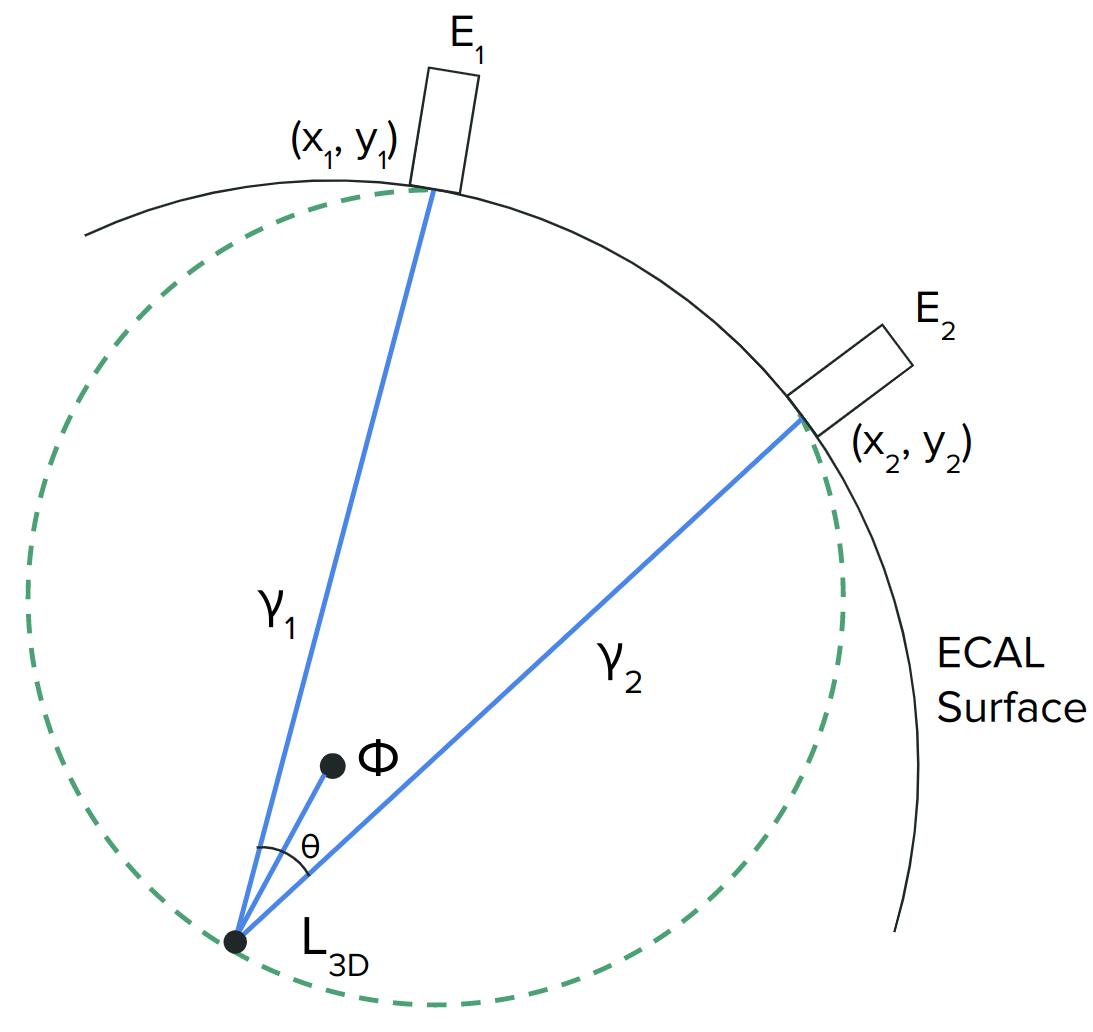
\includegraphics[width=0.65\linewidth]{figs/05_analysis/vertexfit_diagram_negativeLxy.png}
	\caption{Geometrical configuration showing the reconstruction of a negative impact parameter}
	\label{fig:negLxy}
\end{figure}

\subsection{Performance of the Diphoton Vertex Calculation}\label{sec:ana_vertex_results}
It is evident that since the kinematic fit uses the hypothetical mass of the $\Phi$, the fit must be rerun for every hypothetical mass used in this analysis. As a result, the events in the signal region used for each value of $m_\Phi$ are different. Figure~\ref{fig:lxys_a} shows the reconstructed \lxy behaves as expected as the $\Phi$ lifetime increases. To demonstrate the resolution of the kinematic fit, we plot the difference between the calculated \lxy and the generator level \lxy as a function of the generator level \lxy, performed using a $\PZ\to\ell\ell$ samples with m$_\Phi=30\GeV$, using both the c$\tau=100\unit{mm}$ and $1000\unit{mm}$ samples. These distributions can be seen in figure~\ref{fig:lxys_b}. The vertical slices of this histogram were fit to Gaussian distributions so that the mean and sigma could be plotted as a function of generator level \lxy. The means shown in figure~\ref{fig:lxys_c} show the differences in calculated and generator \lxy are compatible with zero, and the sigma shown in figure~\ref{fig:lxys_d} show a resolution of $<3\unit{cm}$, slightly decreasing with generator level $\lxy$. Both the mean and sigma remain consistent across all ranges of m$_\Phi$. The mean has a slight bias towards underestimating the \lxy due to the non-linear relation between the ECAL position/energy resolution and the vertex calculation. The sigma tends to decrease slightly as \lxy increases, as the $\Phi$ decaying closer to the ECAL means the photons traverse less material before reaching the ECAL. This gives a lower probability to interact with the tracker which improves the position and energy resolution.

\begin{figure}[htb!]
	\centering
	\captionsetup[subfigure]{justification=centering}
	\begin{subfigure}[h]{0.45\linewidth}
		\centering
		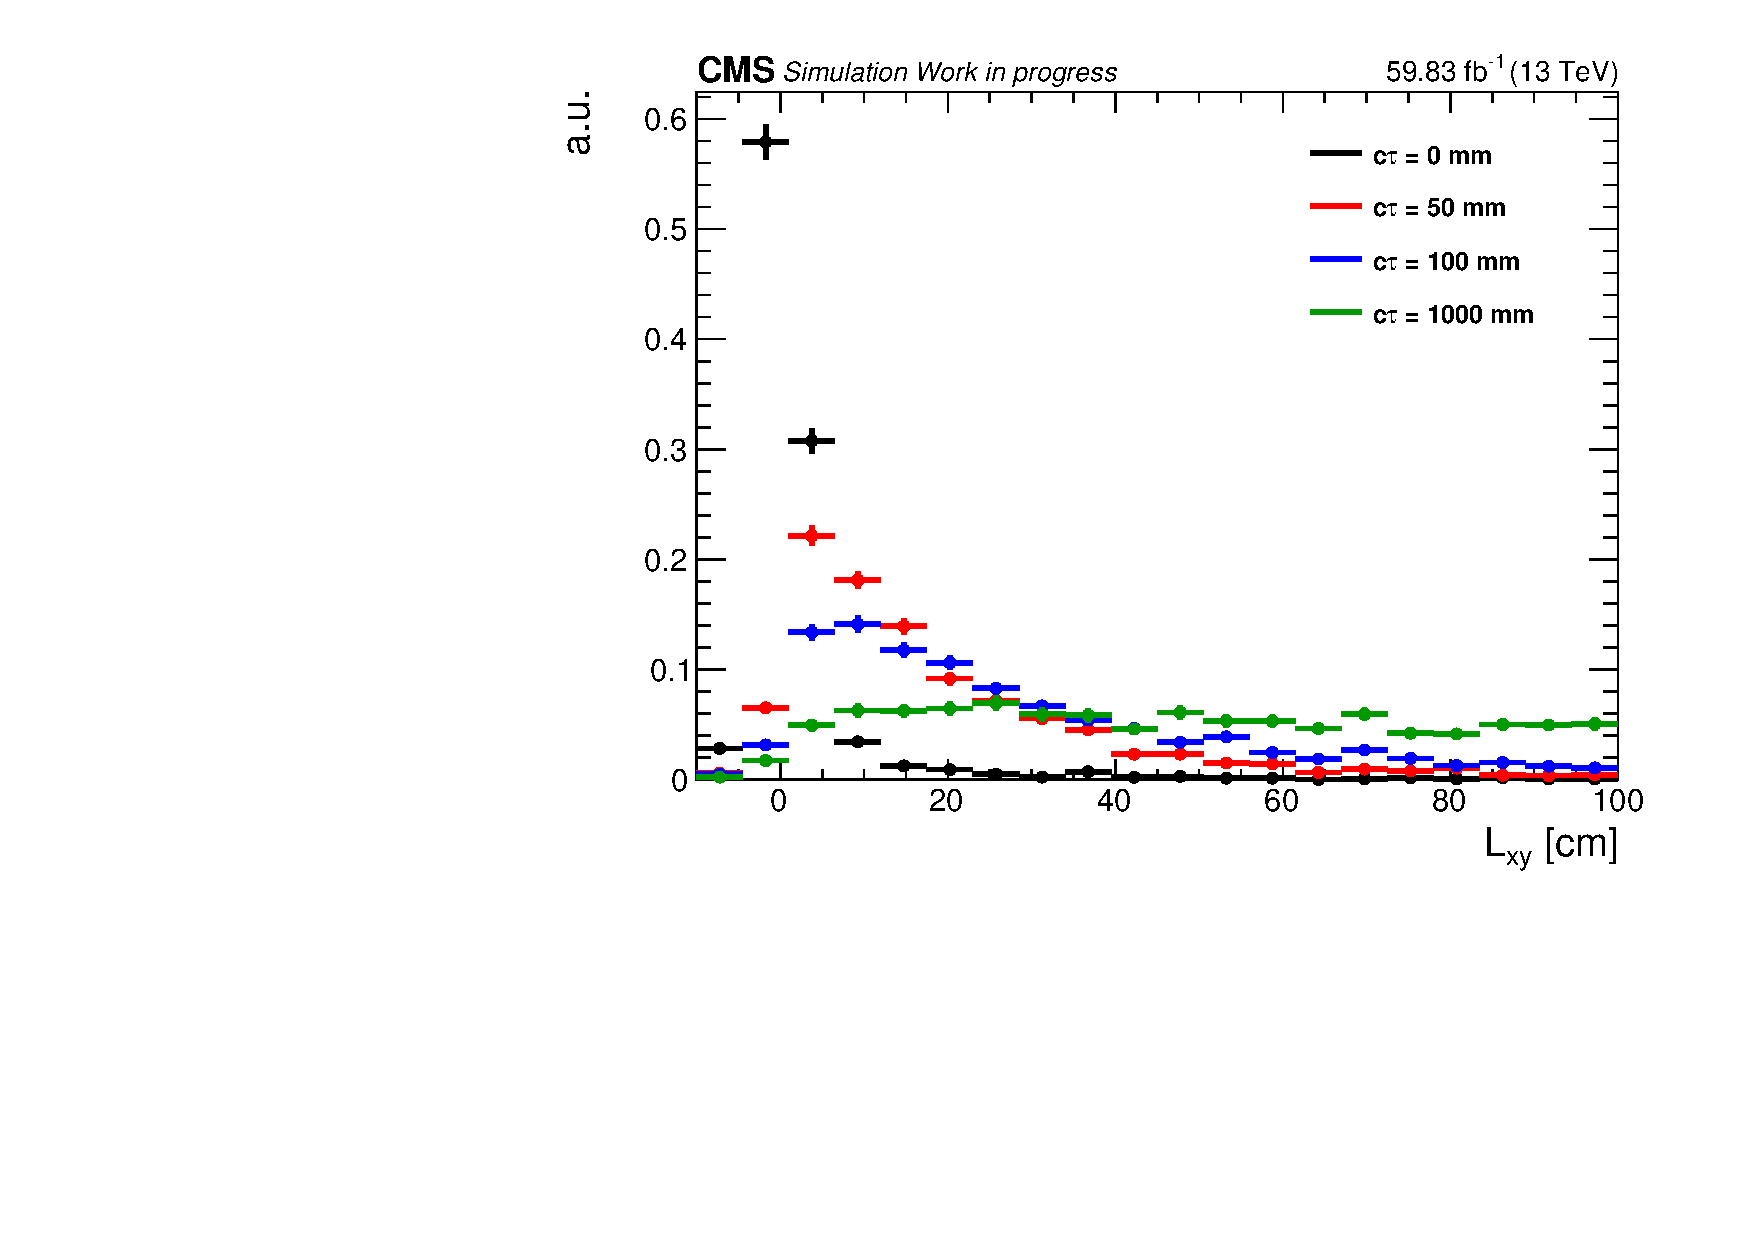
\includegraphics[width=\linewidth]{figs/05_analysis/2018_signalLxy_comparison.pdf}
		\caption{\lxy distribution calculated for $m_\Phi=30\GeV$, $\PZ\to\ell\ell$ signal samples}
		\label{fig:lxys_a}
	\end{subfigure}
	\begin{subfigure}[h]{0.45\linewidth}
		\centering
		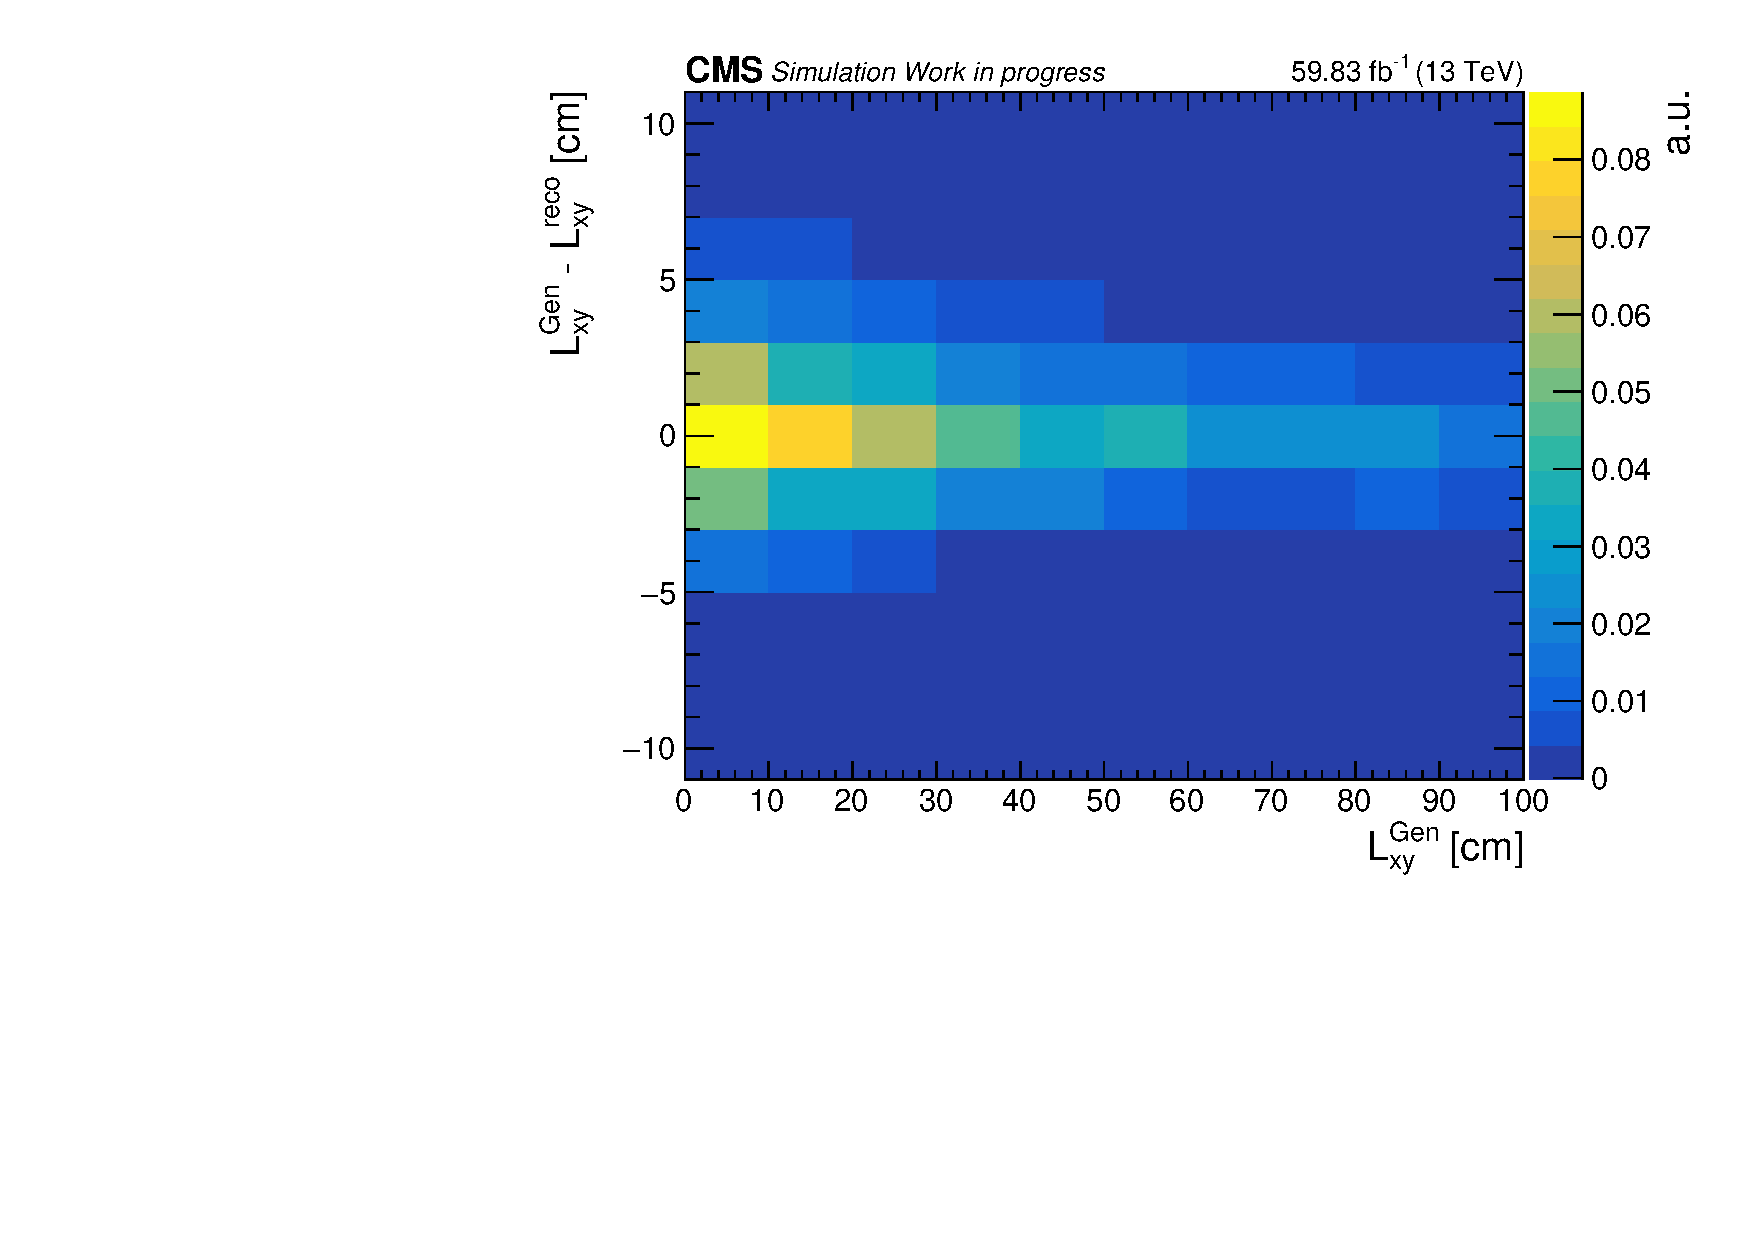
\includegraphics[width=\linewidth]{figs/05_analysis/2018_deltaLxyVsLxy_Z_m30.pdf}
		\caption{The $\Delta\lxy$ vs $\lxy$ distributions for signal events with exactly 2 photons}
		\label{fig:lxys_b}
	\end{subfigure}
	\begin{subfigure}[h]{0.45\linewidth}
		\centering
		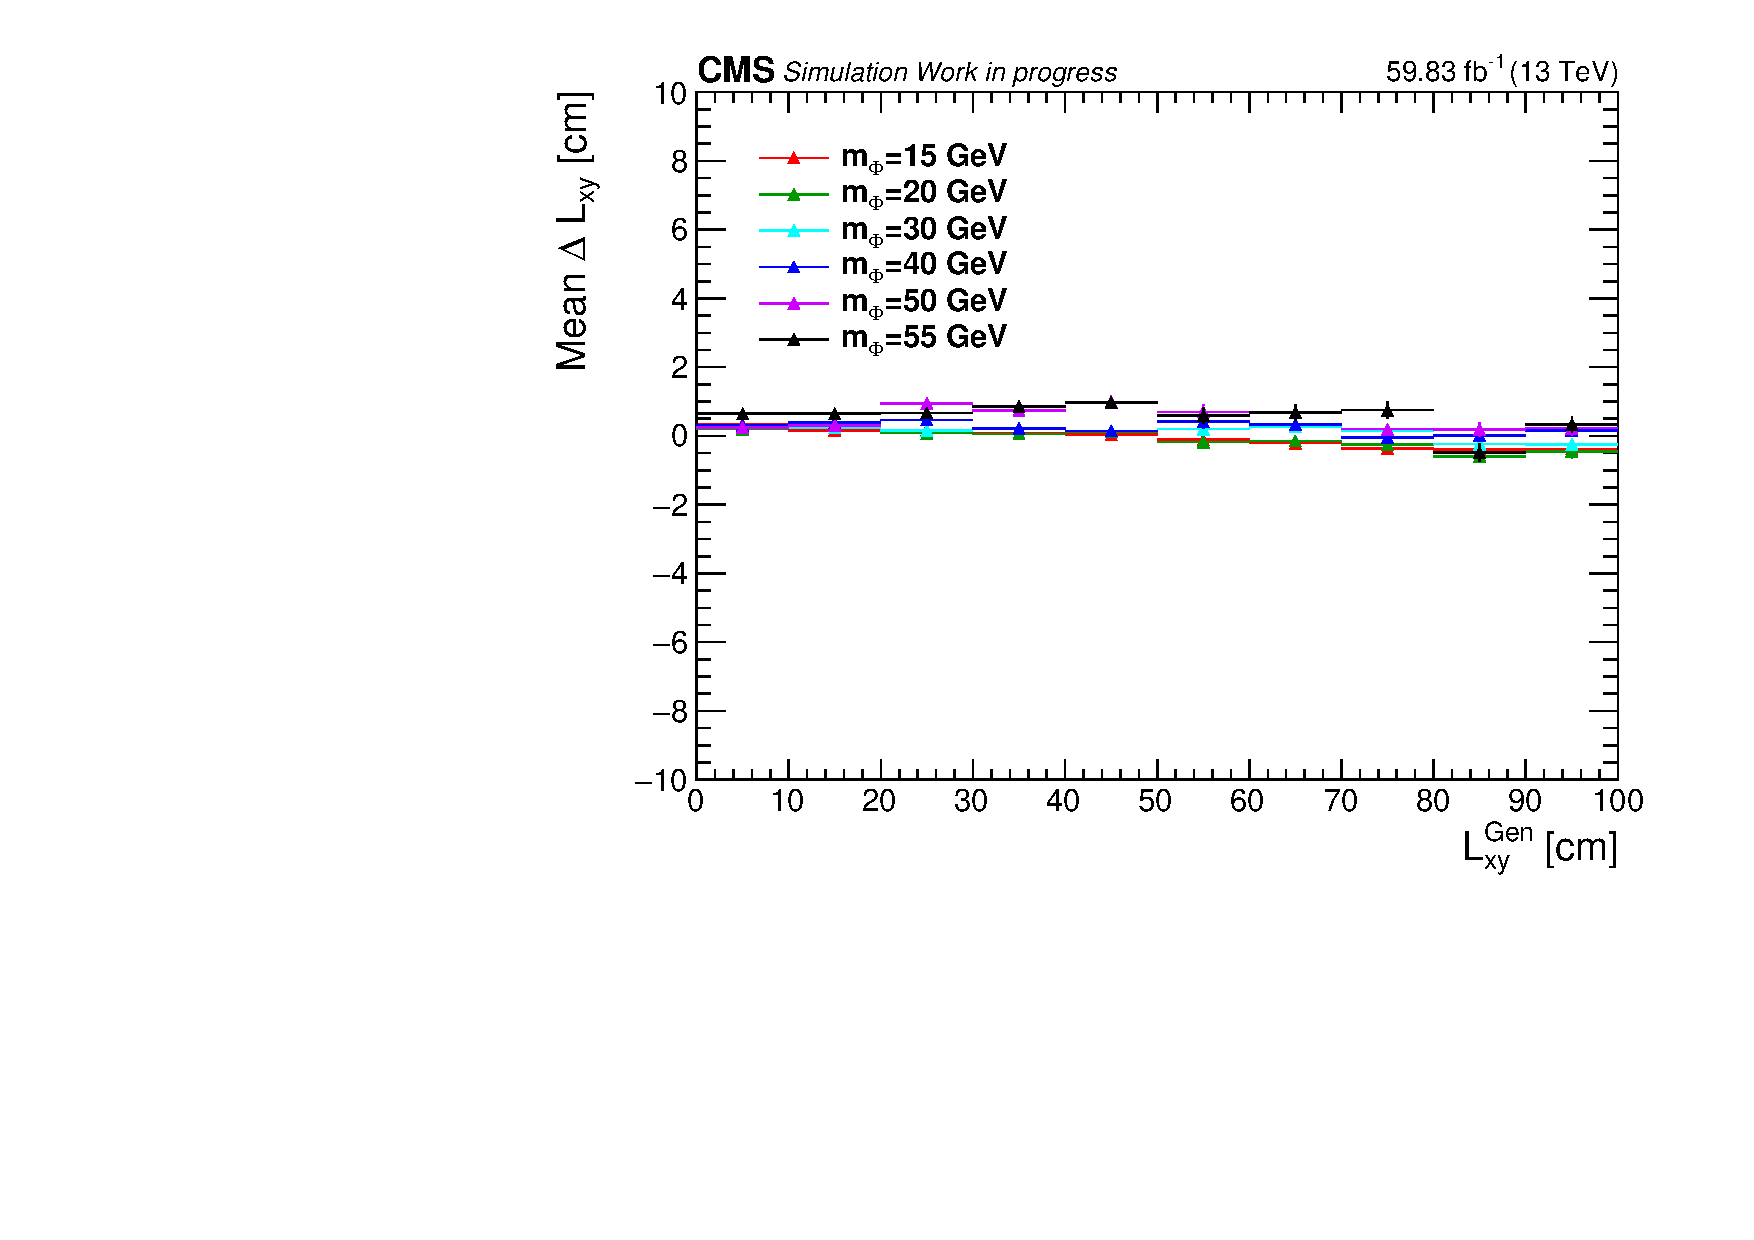
\includegraphics[width=\linewidth]{figs/05_analysis/2018_meanLxyVsLxy_Z_all.pdf}
		\caption{Mean of Gaussian slice fits}
		\label{fig:lxys_c}
	\end{subfigure}
	\begin{subfigure}[h]{0.45\linewidth}
		\centering
		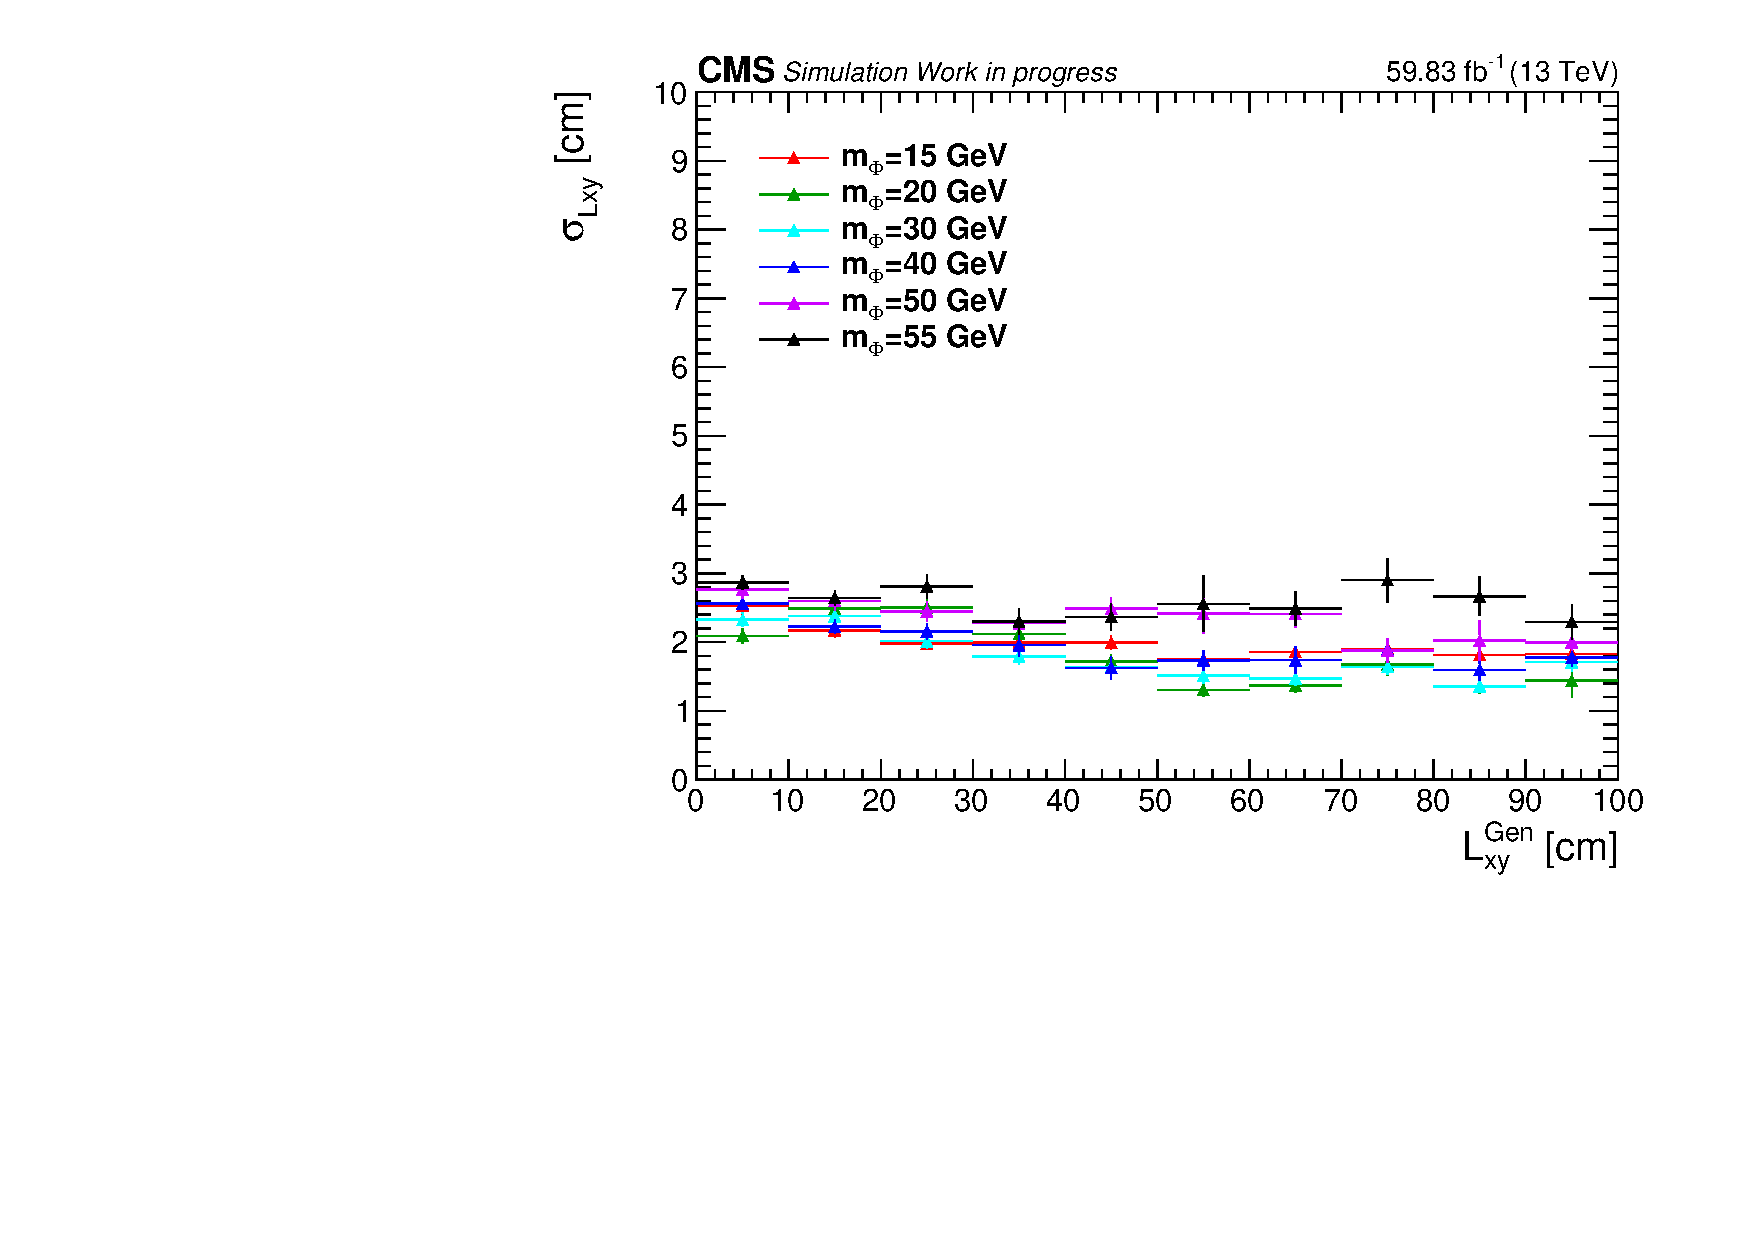
\includegraphics[width=\linewidth]{figs/05_analysis/2018_sigmaLxyVsLxy_Z_all.pdf}
		\caption{Sigma of Gaussian slice fits}
		\label{fig:lxys_d}
	\end{subfigure}
	\caption[Performance of the vertex calculation on signal samples. The fit shows good agreement across all values of generator level \lxy and a resolution of $<3\unit{cm}$.]{Performance of the vertex calculation on signal samples. The fit shows good agreement across all values of generator level \lxy and a resolution of $<3\unit{cm}$.}
	\label{fig:lxys}
\end{figure}

It can be shown that the calculated \lxy for a fixed value of prompt invariant photon mass \mgg is monotonically decreasing with the assumed value of \mphi. Assume that two photons have a prompt (four momenta calculated assuming the two clusters originated from the PV) invariant mass \mgg. Calculating the vertex assuming $\mphi=\mgg$ would yield a vertex with $\lxy=0$ by construction. Calculating the vertex assuming $\mphi>\mgg$ would cause the angle between the two photons given by equation~\ref{eq:me1e2theta} to decrease. As the ECAL cluster positions are fixed, this pushes the vertex backwards yielding $\lxy<0$. By similar methods, assuming a value of $\mphi<\mgg$ yields a vertex with $\lxy>0$. The dependence makes the \lxy very sensitive to small changes in the assumed value of \mphi. If the assumed value of \mphi differs from the true mass by $5\GeV$, the calculated \lxy can skew upwards or downwards by $>20\unit{cm}$, depending on the value of the true mass. Figure~\ref{fig:deltaLxy} shows the differences in generated and reconstructed \lxy, combining samples for all lifetimes for a given true mass.

\begin{figure}[htb!]
	\centering
	\captionsetup[subfigure]{justification=centering}
	\begin{subfigure}[h]{0.45\linewidth}
		\centering
		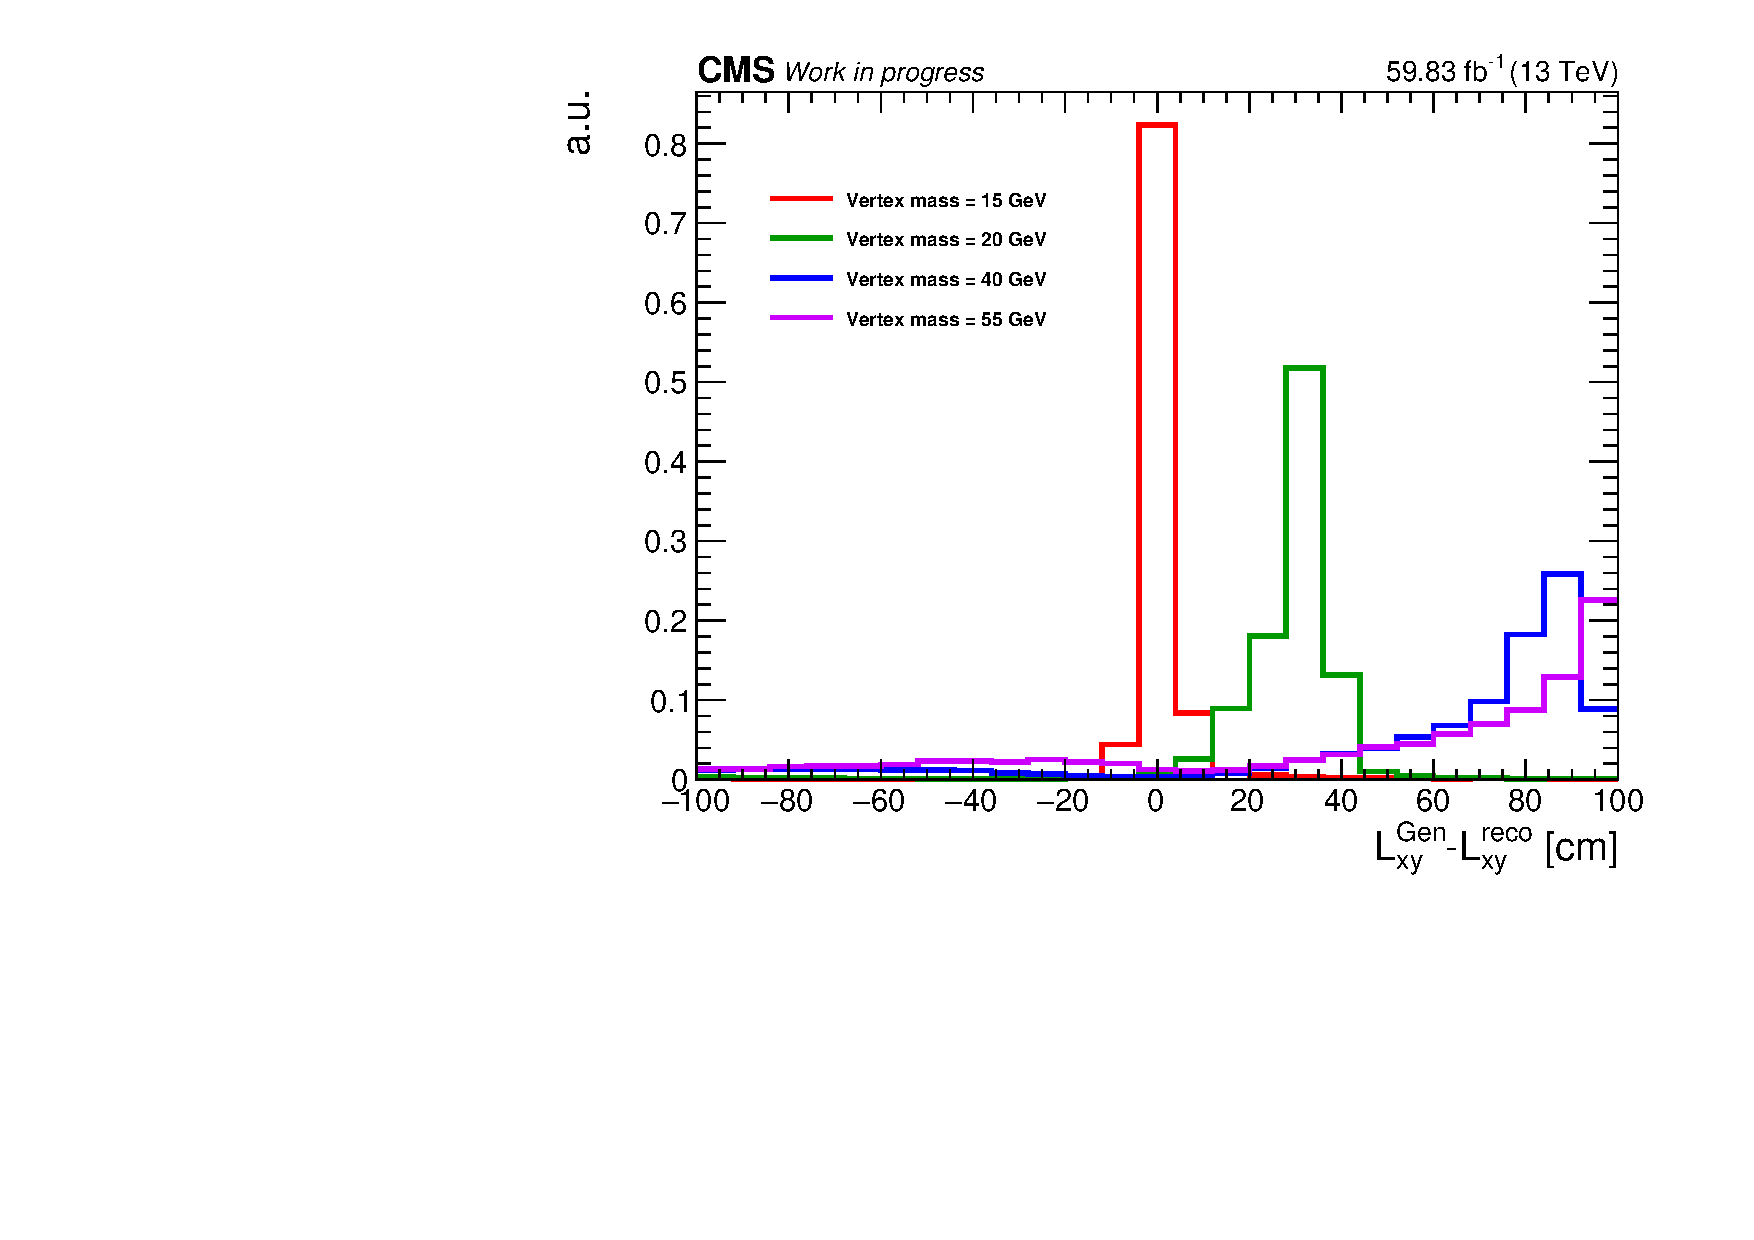
\includegraphics[width=\linewidth]{figs/05_analysis/2018_deltaLxy_Z_m15.pdf}
		\caption{$\mphi=15\GeV$}
	\end{subfigure}
	\begin{subfigure}[h]{0.45\linewidth}
		\centering
		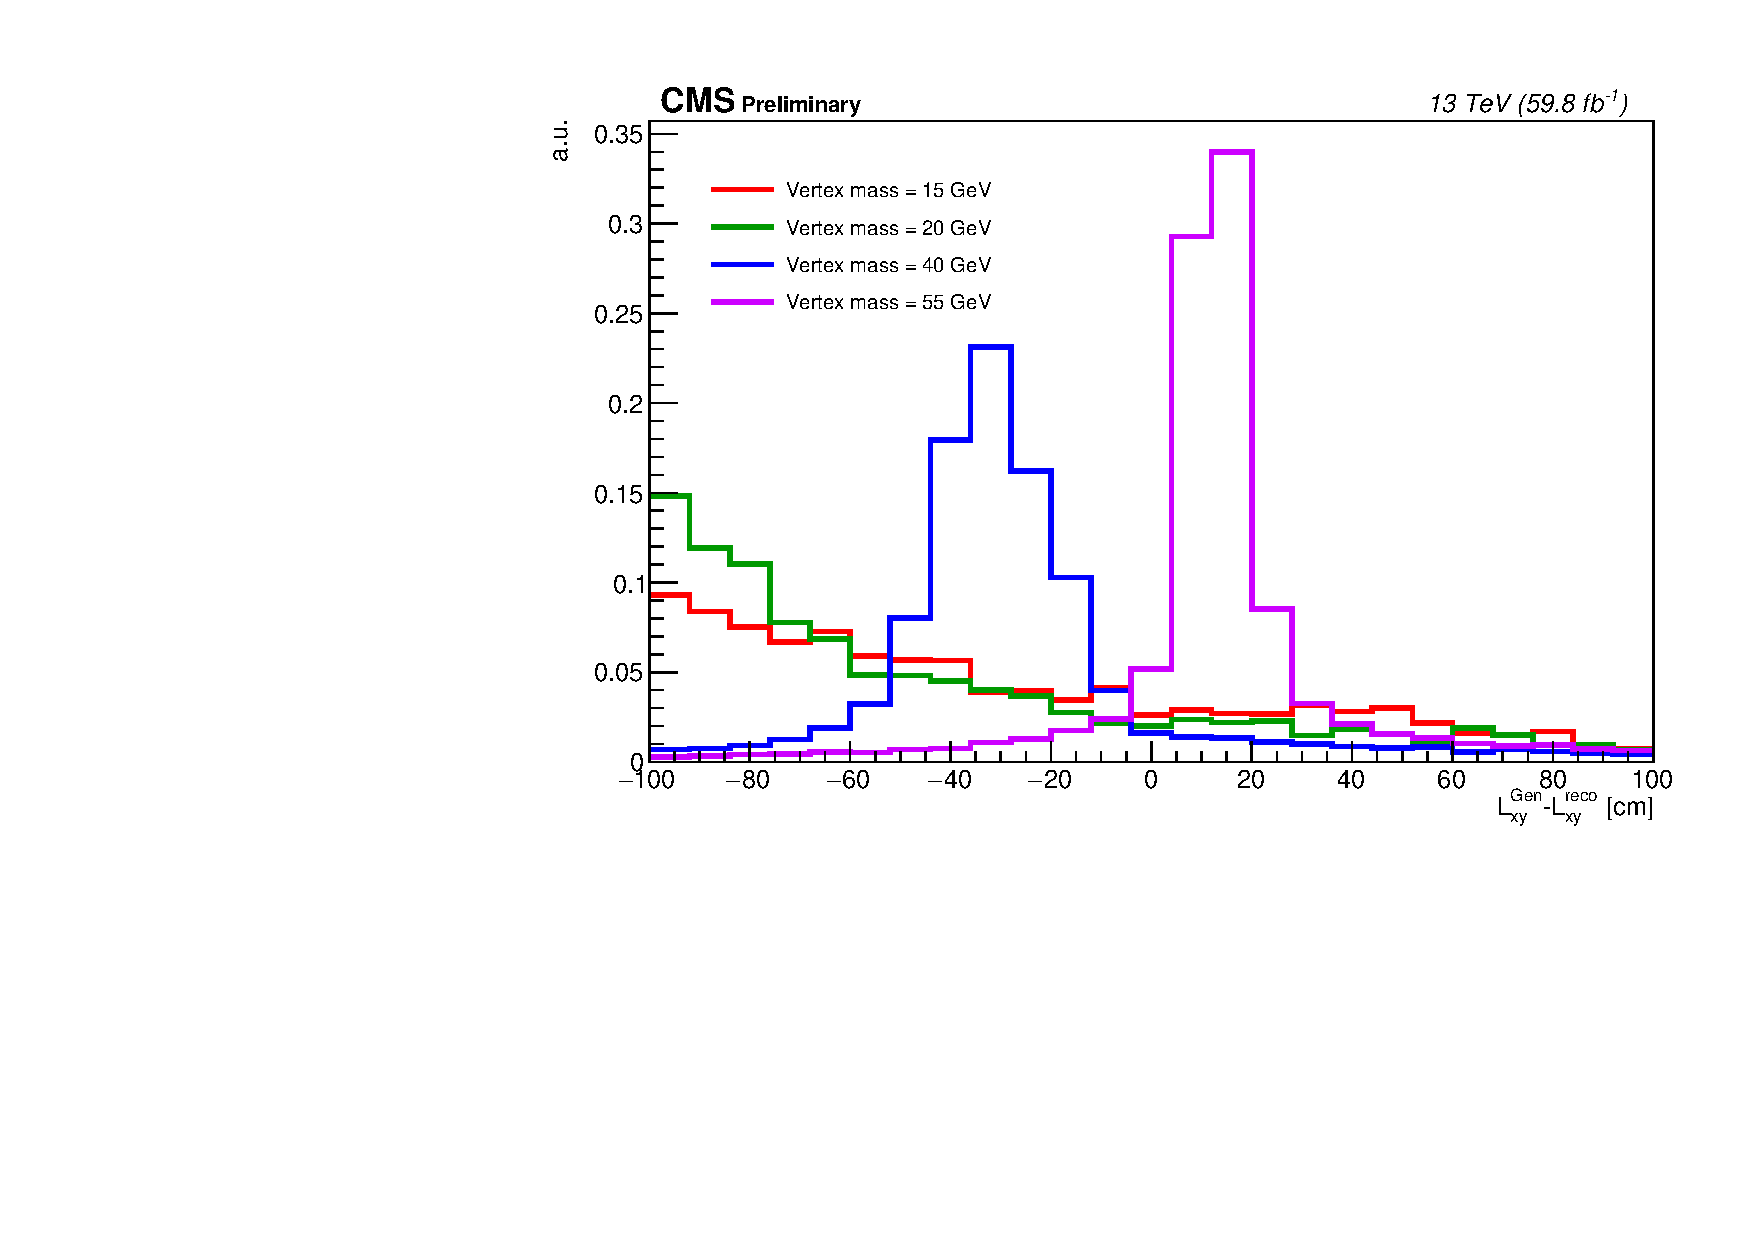
\includegraphics[width=\linewidth]{figs/05_analysis/2018_deltaLxy_Z_m50.pdf}
		\caption{$\mphi=50\GeV$}
	\end{subfigure}
	\caption[The difference between the true and reconstructed vertex grows as the assumed mass departs from the true one. Gen-reconstructed $\lxy$ for a \PZns+\PH samples under several assumed mass points.]{The difference between the true and reconstructed vertex grows as the assumed mass departs from the true one. Gen-reconstructed $\lxy$ for a \PZns+\PH samples under several assumed mass points.}
	\label{fig:deltaLxy}
\end{figure}

The data format used in this analysis is the most slimmed version offered centrally by CMS and provides only the most important information for high level physics objects~\cite{nanoaod}. This information includes several key properties of photons but omits the calorimeter cluster position, which is required to calculate the diphoton vertex. To circumvent this, we propagate the photons from the PV to the ECAL using their $\eta$ and $\phi$. The ECAL is approximated using a cylinder with radius $\rho=137\unit{cm}$ and $z=324\unit{cm}$. These values are shown in figure~\ref{fig:calo_position}. Diphoton vertices calculated using the propagated coordinates yield a \lxy within 3\% of the \lxy calculations using the exact cluster coordinates, which is well within the intrinsic resolution of the vertex calculation.

\begin{figure}[htb!]
	\centering
	\captionsetup[subfigure]{justification=centering}
	\begin{subfigure}[h]{0.45\linewidth}
		\centering
		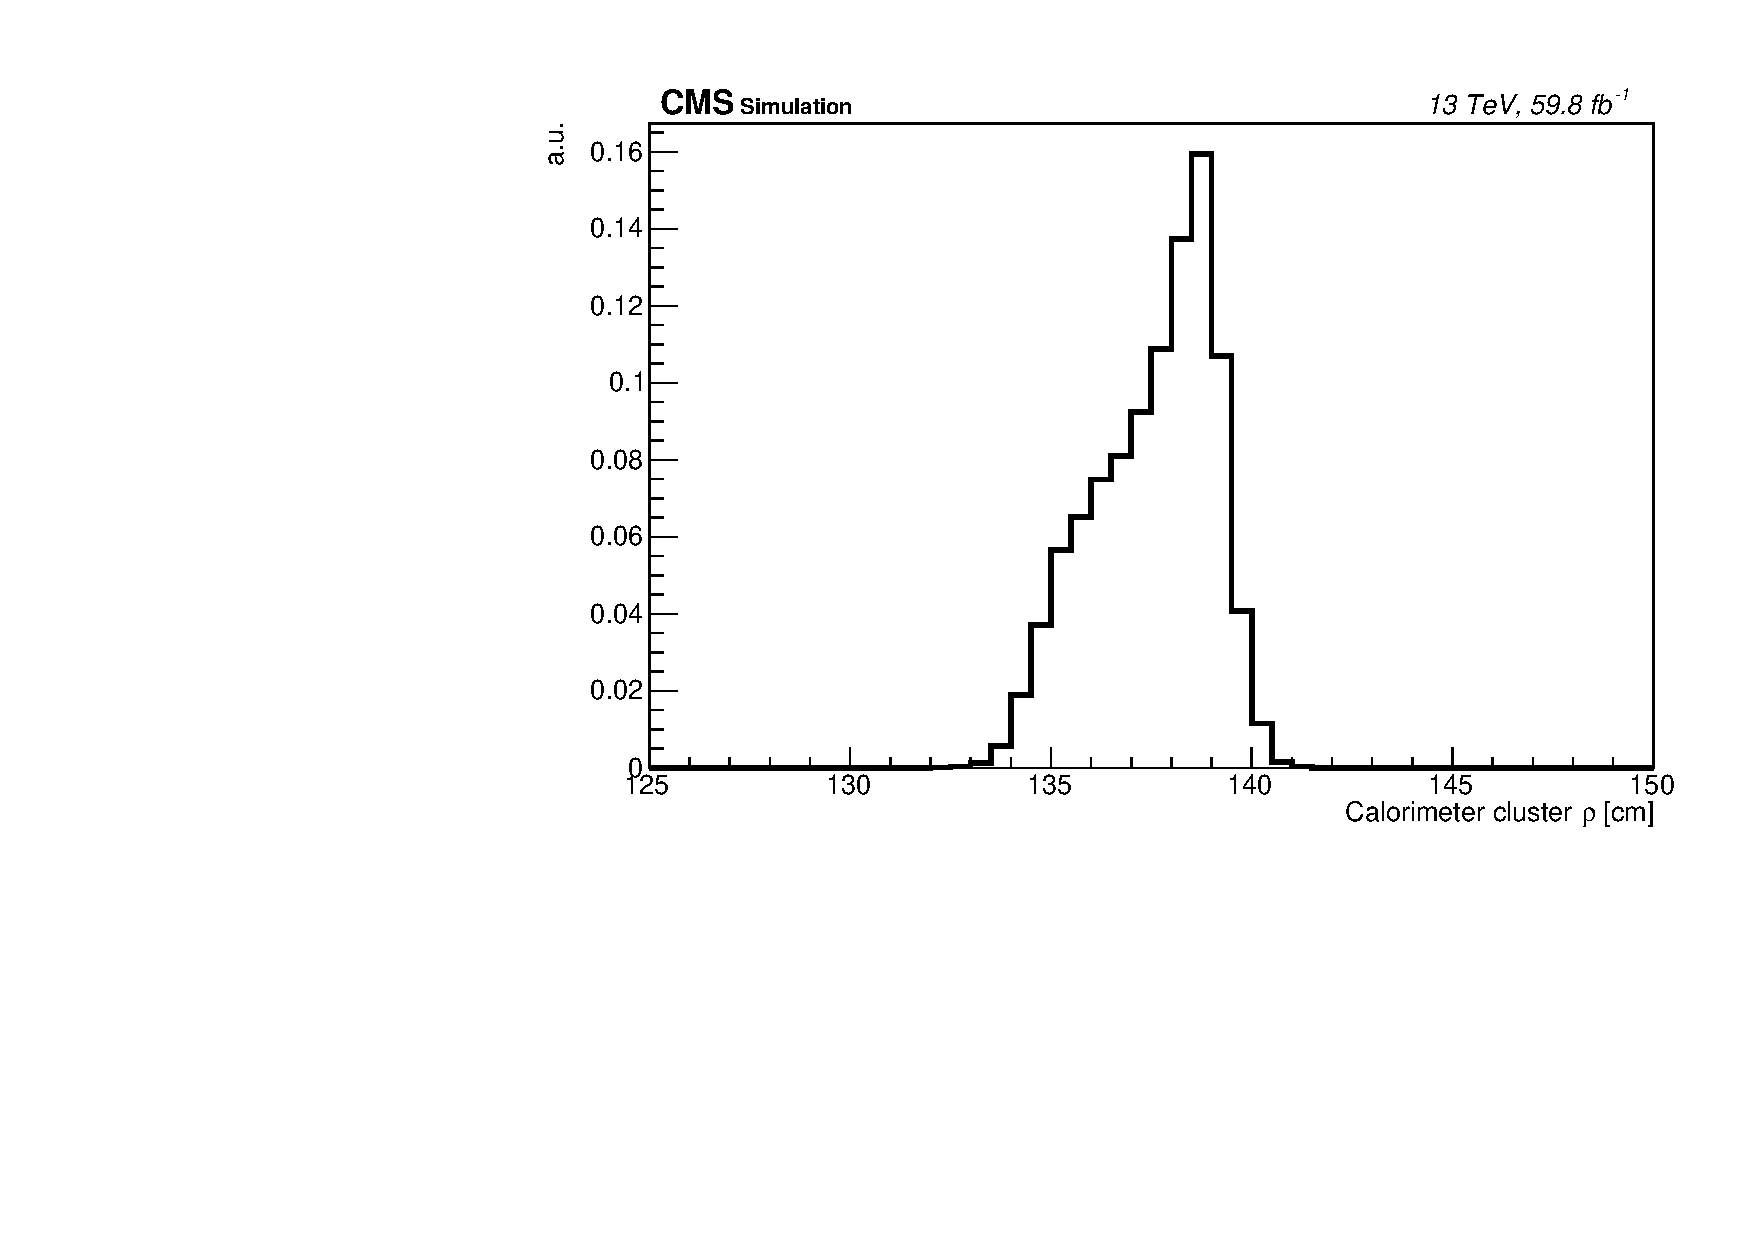
\includegraphics[width=\linewidth]{figs/05_analysis/calorimeter_rho.pdf}
		\caption{Calormieter cluster $\rho$}
	\end{subfigure}
	\begin{subfigure}[h]{0.45\linewidth}
		\centering
		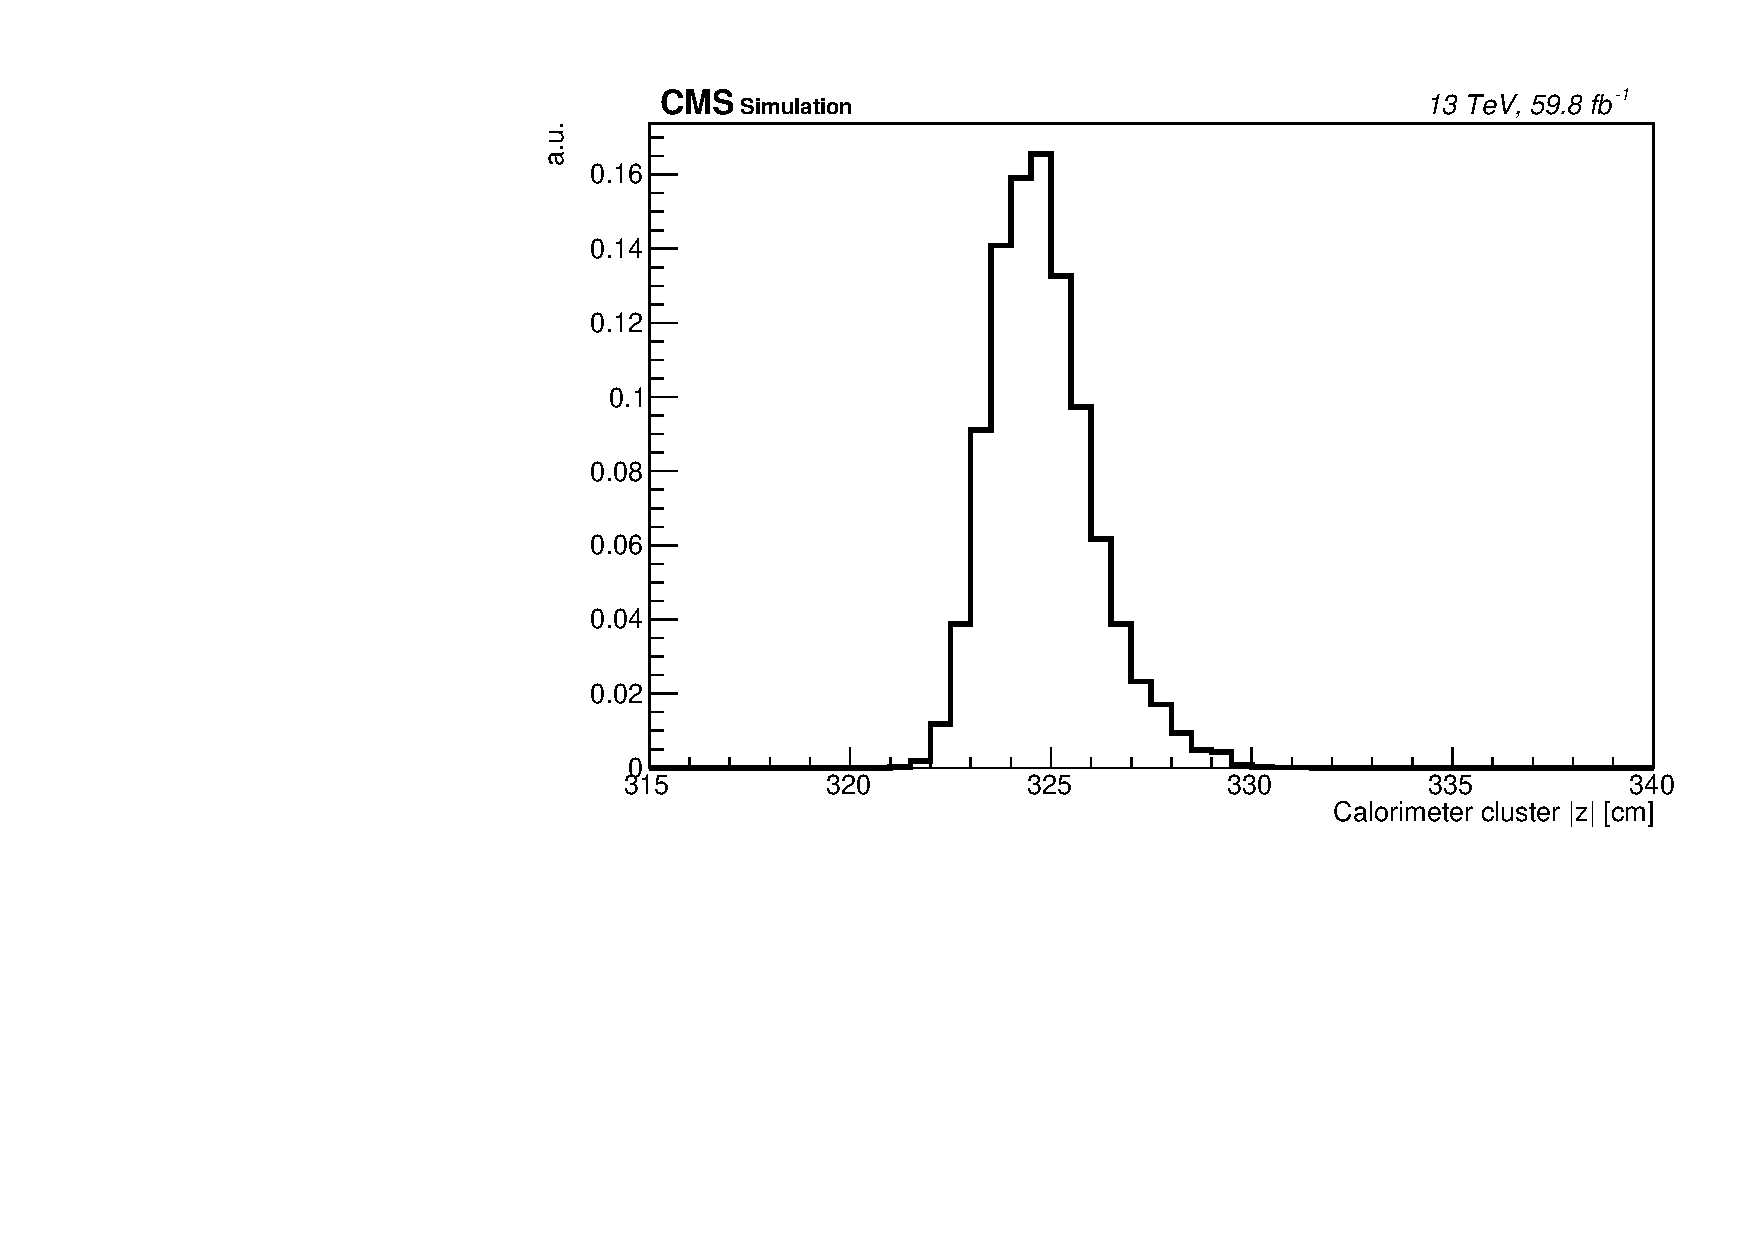
\includegraphics[width=\linewidth]{figs/05_analysis/calorimeter_z.pdf}
		\caption{Calorimeter cluster $|z|$}
	\end{subfigure}
	\caption[The $\rho$ for barrel photons and $|z|$ for endcap photons for all reconstructed photons.]{The $\rho$ for barrel photons and $|z|$ for endcap photons for all reconstructed photons.}
	\label{fig:calo_position}
\end{figure}

\section{Event Selection} \label{sec:ana_eventsel}
The first step in collecting events for the analysis is to select events passing HLT lepton triggers. Events passing these triggers are then chosen based on the presence of two same flavor, opposite charge leptons and two photons. Various quality cuts, referred to as preselection criteria, are applied to these objects to reject background. Lastly, event level cuts are applied to reject photons from final state radiation (FSR) and low \pt photons that get promoted to displaced $\Phi$ candidates by the kinematic vertex fit.

\subsection{Triggers} \label{sec:ana_triggers}
Events are triggered through leptonic decays of the \PZ boson produced in association with the SM Higgs Boson. The \PZ candidates are selected from dilepton events passing the HLT isolated single lepton triggers. These triggers are the standard lepton triggers recommended both the EGamma and Muon physics object groups (POGs) in CMS. Double lepton and high \pt lepton triggers were considered but provide only negligible improvement when applied in addition to the single lepton triggers. To ensure events are not double counted between data sets, muon events must pass the single muon triggers and are vetoed by the single electron triggers, while electron events must pass single electron triggers and are vetoed by the single muon triggers. A complete list of HLT trigger paths used for each year can be see in table~\ref{tab:triggers}.

\begin{table}[h]
	\caption[HLT trigger paths used for the Run 2 datasets]{HLT trigger paths used for the Run 2 datasets} 
	\label{tab:triggers}
	\begin{center}
		\begin{tabular}{l|l|l}\hline
			Year & Single Electron & Single Muon\\
			\hline
			2018 & HLT\_Ele32\_WPTight\_Gsf & HLT\_IsoMu24\\
			2017 & HLT\_Ele32\_WPTight\_Gsf & HLT\_IsoMu27\\
			2016 & HLT\_Ele27\_WPTight\_Gsf & HLT\_IsoMu24 \textbar\textbar HLT\_IsoTkMu24\\
			\hline
		\end{tabular}
	\end{center}
\end{table}

Each HLT path name corresponds to the different criteria required to pass the trigger. The electron triggers require the trigger object have $\pt>32\GeV$ ($27\GeV$ for 2016), pass tight selection criteria, and be reconstructed using the Gaussian sum filter (GSF) algorithm discussed in section~\ref{sec:CMS_reco_egamma}. Muons are required to pass isolation and have $\pt>24\GeV$ ($27\GeV$ for 2017). In order to improve the efficiency of the muon trigger in 2016, we also include the tracker muon trigger, which requires an isolated tracker muon with $\pt>24\GeV$.

\subsection{Preselection Criteria} \label{sec:ana_preselection}
For both electrons and muons we define a set of tight and loose leptons based on cut based ID set by the EGamma and Muon POGs. To reconstruct a \PZ candidate, we require exactly two same flavor opposite charge tight leptons with invariant mass $70<m_{\ell\ell}<110\GeV$ and zero additional loose leptons. For photons we require at least two photons passing a set of preselection criteria, which are subject to additional classification based on cut based ID.

\subsubsection{Particle Flow Isolation} \label{sec:ana_isolation}
One key application of the particle flow (PF) algorithm is the calculation of a particle's isolation. This quantity measures the \pt and energy contributions from PF candidates in a fixed $\Delta R$ cone centered on the original particle. A lower value implies the particle is more isolated (i.e. there are fewer additional particles nearby), and vice versa. Isolation is a key variable to reject particles produced in jets from heavy-flavor hadronic decays or decays of pions and kaons~\cite{Sirunyan:PF}. A particle's isolation is defined as follows:
\begin{equation}
	\label{eq:pfiso}
	I_\text{pf} = \sum_{\substack{i\in\text{charged}\\\text{hadrons}}}\pt^i+\text{max}\left(0,\sum_{\substack{i\in\text{neutral}\\\text{hadrons}}}\et^i+\sum_{\gamma\in\text{photons}}\et^\gamma-\text{PU Corrections}\right)
\end{equation}

The three contributions that are summed over in equation~\ref{eq:pfiso} are referred to as charged hadron isolation ($I_\text{ch}$), neutral hadron isolation ($I_\text{n}$), and photon isolation ($I_\gamma$). It is also common to refer to a particle's isolation normalized by its \pt (or $E_\mathrm{T}$ for neutral particles), known as relative isolation which is defined as
\begin{equation}
	\label{eq:reliso}
	I_\text{rel}=\frac{I_\text{pf}}{\pt}
\end{equation}

Particles created from pileup can create calorimeter deposits within the $\Delta R$ cone used to calculate isolation. These are unrelated to the physics process for the central particle and can artificially inflate the isolation. Only charged hadrons with tracks originating from the PV are used when calculating the charged hadron isolation, which rejects charged hadrons originating from PU. Neutral particles, however, do not produce tracks, meaning calorimeter deposits from the PV and from pileup are indistinguishable. Because of this, there are additional corrections to remove the PU contributions from neutral hadron and photon isolation. Two common methods are $\rho$ corrections, which calculate the average energy density per unit area from pileup ($\rho$) multiplied by an effective area as a function of $\eta$, and $\Delta\beta$ corrections, which calculate the energy from photons and neutral hadrons in pileup as a fraction of the charged hadron contribution from PU.

\subsubsection{Muon Criteria} \label{sec:ana_muons}
The data format used for this analysis takes reconstructed muons and applies loose cuts before storing the muon properties in branches. These branches contain all muons with $\pt>3\GeV$ with minimal cuts to reconstruction quality. For the purpose of this analysis, muons are classified as loose if they pass all of the following criteria:
\begin{itemize}
	\item $\pt>10\GeV$
	\item $|\eta|<2.4$
	\item $D_{xy}<0.2\unit{cm}$: the transverse distance from the PV to the beamline must be less than 0.2 cm
	\item $D_{z}<0.5\unit{cm}$: the longitudinal distance from the PV to the beamline must be less than 0.5 cm
	\item $I_\text{rel}(\Delta R<0.4,\,\Delta\beta\text{-corrected})<0.25$
	\item Passes loose quality criteria set by the Muon POG:
	\begin{itemize}
		\item Muon must be reconstructed by the PF algorithm
		\item Muon must be either a global and/or tracker muon
	\end{itemize}
\end{itemize}
We define tight muons as a subset of loose muons if they pass the following criteria:
\begin{itemize}
	\item $I_\text{rel}(\Delta R<0.4,\,\Delta\beta\text{-corrected})<0.15$
	\item Passes tight quality criteria set by the Muon POG:
	\begin{itemize}
		\item Muon must be a global muon
		\item The global muon track fit must have $\chi^2/\text{ndof}<10$
		\item Global track must have at least one hit in a muon chamber %TODO: why is this necessary if it's already a global muon?
		\item Muon track must have segments in at least 2 different muon stations %TODO: same question
		\item Tracker track $D_{xy}<2\unit{mm}$
		\item Tracker track $D_{z}<5\unit{mm}$
		\item Tracker track must have at least 1 hit in the pixel detector
		\item Tracker track must have hits in more than 5 tracker layers
	\end{itemize}
\end{itemize}
We also require that one of the two tight muons used to reconstruct the \PZ be the triggering muon, and that the triggering muon have $\pt>25\GeV$ ($28\GeV$ in 2017) in order to operate above the single muon trigger \pt thresholds.

\subsubsection{Electron Criteria} \label{sec:ana_electrons}
Analogously to the muon criteria, loose electrons are defined from reconstructed electrons if they pass a set of preselection criteria. 
\begin{itemize}
	\item $\pt>15\GeV$
	\item $|\eta|<2.4$
	\item $|\eta|>1.57\text{ or }|\eta|<1.44$ to rejects clusters in the overlap region between the ECAL barrel and endcap
	\item $D_{xy}<0.2\unit{cm}$, $D_{z}<0.2\unit{cm}$
	\item Passes cut based ID provided by the EGamma POG at the \texttt{veto} working point
\end{itemize}
Tight electrons are selected from this collection of they pass cut based ID at the \texttt{tight} working point set by the EGamma POG. A full set of criteria is shown in table~\ref{tab:electronID} for barrel and endcap electrons. Similar to the muon criteria, we require one of the tight electrons be the triggering electron, and that the triggering electron have $\pt>35\GeV$.

\begin{table}[htb!]
	\centering
	\caption[Cut based ID selection criteria for electrons in Run-2.]{Cut based ID selection criteria for electrons in Run-2~\cite{electronid}.}
	\label{tab:electronID}
	\subcaption{Barrel Electrons}
	\begin{tabular}{l | r | r}
		\hline
		Barrel Criteria & Veto & Tight \\
		\hline
		\hline
		$\sigma_{i\eta i\eta}<$ & 0.0126 & 0.0104 \\
		$|\Delta\eta_\text{seed}|<$ & 0.0463 & 0.00255 \\
		$|\Delta\phi_\text{In}|<$ & 0.148 & 0.022 \\
		$H/E<$ & $0.05+1.16/E+0.0324\rho/E$ & $0.026+1.15/E+0.0324\rho/E$ \\
		$I_\text{rel}(\Delta R<0.3,\rho\text{ corrected})<$ & $0.198+0.506/\pt$ & $0.0287+0.506/\pt$\\
		$|1/E-1/p|<$  & 0.209 & 0.159 \\
		Missing inner hits $\leq$ & 2 & 1 \\
		Passes conversion veto & True & True\\
		\hline
	\end{tabular}
	\centering
	\subcaption{Endcap Electrons}
	\begin{tabular}{l | r | r}
		\hline
		Endcap Criteria & Veto & Tight \\
		\hline
		\hline
		$\sigma_{i\eta i\eta}<$ & 0.0457 & 0.0353 \\
		$|\Delta\eta_\text{seed}|<$ & 0.00814 & 0.00501 \\
		$|\Delta\phi_\text{In}|<$ & 0.19 & 0.0236 \\
		$H/E<$ & $0.05+2.54/E+0.183\rho/E$ & $0.0188+2.06/E+0.183\rho/E$ \\
		$I_\text{rel}(\Delta R<0.3,\rho\text{ corrected})<$ & $0.203+0.963/\pt$ & $0.0445+0.963/\pt$\\
		$|1/E-1/p|<$ & 0.132 & 0.0197 \\
		Missing inner hits $\leq$ & 3 & 1 \\
		Passes conversion veto & True & True\\
		\hline
	\end{tabular}
\end{table}

The variables used in the cut based ID are optimized to reject background such as photons in hadronic showers or photons that convert to $e^+e^-$ pairs in the tracker. The spread of the calorimeter cluster in $\eta$ is measured using $\sigma_{i\eta i\eta}$, which is the weighted second moment of the cluster shape in $\eta$ measured in a $5\times5$ grid of calorimeter crystals, centered on the most energetic crystal in the SC. This variable can be used to discriminate two photon showers produced from neutral meson decays, which have higher spread in $\eta$, from showers produced by prompt electrons or photons. The $H/E$ ratio takes the energy of HCAL clusters located in a $\Delta R<0.15$ cone behind the ECAL cluster and divides it by the ECAL cluster energy. Genuine EM showers have three main contributions to hadronic energy: leakage through gaps into the HCAL, calorimeter noise, and pileup. The constant term in these cuts accounts for energy leakage from real electrons or photons, the term proportional to $1/E$ is to account for noise in the HCAL, and the $\rho/E$ term is the correction due to pileup. Tracker information is also used to separate signal from background. The $|\Delta\eta_\text{seed}|$ and $|\Delta\phi_\text{in}|$ are the difference in SC and track $\eta$/$\phi$, measured from the innermost tracker layer, which is expected to be small for prompt electrons. The difference between tracker momentum and calorimeter energy is measured using the quantity $|1/E-1/p|$, which should be small as a good electron should have similar energy and momentum. The number of missing hits refers to number of gaps in the electron's trajectory through the tracker. Converted photons will leave tracks after the conversion vertex but leave no hits in the tracker before they convert, while prompt electrons should leave hits in the tracker starting from the PV. An additional conversion veto is applied by rejecting electrons with tracks matched to conversion vertices in order to further reject background from converted photons. The tight cut based ID is expected to have a 70\% signal efficiency for real electrons.

\subsubsection{Photon Criteria} \label{sec:ana_photons}
Similar to the muons, reconstructed photons must pass baseline selection to be stored in the data format used by this analysis. All reconstructed photons must have $\pt>5\GeV$, $R_9>0.8$, and pass cuts on total and relative charged hadron isolation given by $I_\text{ch}<20\GeV$ and $I_\text{ch}/\pt<0.3$. The $R_9$ of a supercluster is defined as the energy the most energetic $3\times3$ crystal grid in the supercluster divided by the total supercluster energy. For an event to be considered for this analysis, we require at least two nanoAOD photons passing the following preselection criteria:
\begin{itemize}
	\item $\pt>20\GeV$
	\item Passes pixel seed veto
	\item $|\eta|<2.4$
	\item $|\eta|>1.57\text{ or }|\eta|<1.44$
	\item $\Delta\eta$($\gamma$, lepton)$^2$/0.4$^2$ + $\Delta\varphi$($\gamma$, lepton)$^2$/0.5$^2$ $>$ 1 for all loose leptons
\end{itemize}

Due to the production mechanism of the Higgs boson, the $\Phi$ and subsequent photon pair are expected to be strongly correlated and have high energy. The following kinematic requirements based on the four-momentum of the diphoton system reject background due to uncorrelated or lower energy photon pairs while maintaining 99\% signal efficiency:
\begin{itemize}
	\item $\pt(\gamma,\gamma)>20\GeV$
	\item Invariant diphoton mass $\mgg>4\GeV$
\end{itemize}

The pixel seed veto reject photons if there are at least two pixel seed hits that point to the supercluster, which is used to reject background from electrons that are misidentified as photons. Photons passing this preselection criteria are subject to further classification as ID'd or anti-ID'd if they pass or fail loose cut based ID outlined in table~\ref{tab:photonID}. The loose ID is measured to have approximately 90\% efficiency for prompt photons, but was observed to have additional inefficiencies due to photon isolation and shower shape variables resulting from the displaced signature of the two photons. As the photon vertex becomes more displaced, the shower shape becomes more skewed and the two photons become closer together, which affects the cuts to $\sigma_{i\eta i\eta}$ and $I_\gamma$. At lower masses, the photon isolation is the main source of inefficiency because the photons are more collimated, while at higher masses the $\sigma_{i\eta i\eta}$ is the main inefficiency as the larger angle between the photons causes a larger spread in shower shape. The effect of each criteria in the cut based ID on the photon reconstruction efficiency is shown as a function of generator level \lxy in figure~\ref{fig:Photon_cutBased} for all values of \mphi. The efficiency denominator is all generator level (gen) photon pairs, where each gen photon has $\pt>20\GeV$ and a decay vertex within the CMS ECAL. The numerator requires each gen photon to have a matching reconstructed photon that passes given selection criteria. Matching requires the reconstructed photon have $\Delta R < 0.3$ and energy within 50\% of the gen photon.

Given the large inefficiency of the $I_\gamma$ cuts at low values of $\mphi$, studies were performed using modified photon isolation by removing the footprint of the partner photon from $I_\gamma$. This modified ID showed up to 50\% improvement in signal efficiency for low \mphi, high \lxy events. However, this was shown to introduce substantial irreducible background with only marginal improvements to expected limits, so it was not used in the final analysis.

\begin{table}[htb!]
	\centering
	\caption[Cut based ID selection criteria for photons in Run-2.]{Cut based ID selection criteria for photons in Run-2~\cite{photonid}.}
	\label{tab:photonID}
	\begin{tabular}{l | l}
		\hline
		Barrel Criteria & Loose ID \\
		\hline
		\hline
		$H/E<$ & 0.04596\\
		$\sigma_{i\eta i\eta}<$ & 0.0106\\
		$I_\text{ch}(\Delta R<0.3,\rho\text{ corrected})<$ & 1.694\\
		$I_\text{n}(\Delta R<0.3,\rho\text{ corrected})<$ & $24.032+0.01512*\pt+2.259*10^{-5}*\pt^2$\\
		$I_\gamma(\Delta R<0.3,\rho\text{ corrected})<$ & $2.876+0.004017*\pt$\\
		\hline
		\multicolumn{2}{l}{}\\
		\hline
		Endcap Criteria & Loose ID \\
		\hline
		\hline
		$H/E<$ & 0.0590\\
		$\sigma_{i\eta i\eta}<$ & 0.0272\\
		$I_\text{ch}(\Delta R<0.3,\rho\text{ corrected})<$ & 2.089\\
		$I_\text{n}(\Delta R<0.3,\rho\text{ corrected})<$ & $19.722+0.01512*\pt+2.3*10^{-5}*\pt^2$\\
		$I_\gamma(\Delta R<0.3,\rho\text{ corrected})<$ & $4.162+0.0037*\pt$\\
		\hline
	\end{tabular}
\end{table}

\begin{figure}[htb!]
	\centering
	\begin{tabular}{>{\centering\arraybackslash}m{0.32\linewidth} >{\centering\arraybackslash}m{0.32\linewidth} >{\centering\arraybackslash}m{0.32\linewidth}}
		$\mphi=15\GeV$ & $\mphi=20\GeV$ & $\mphi=30\GeV$ \\
		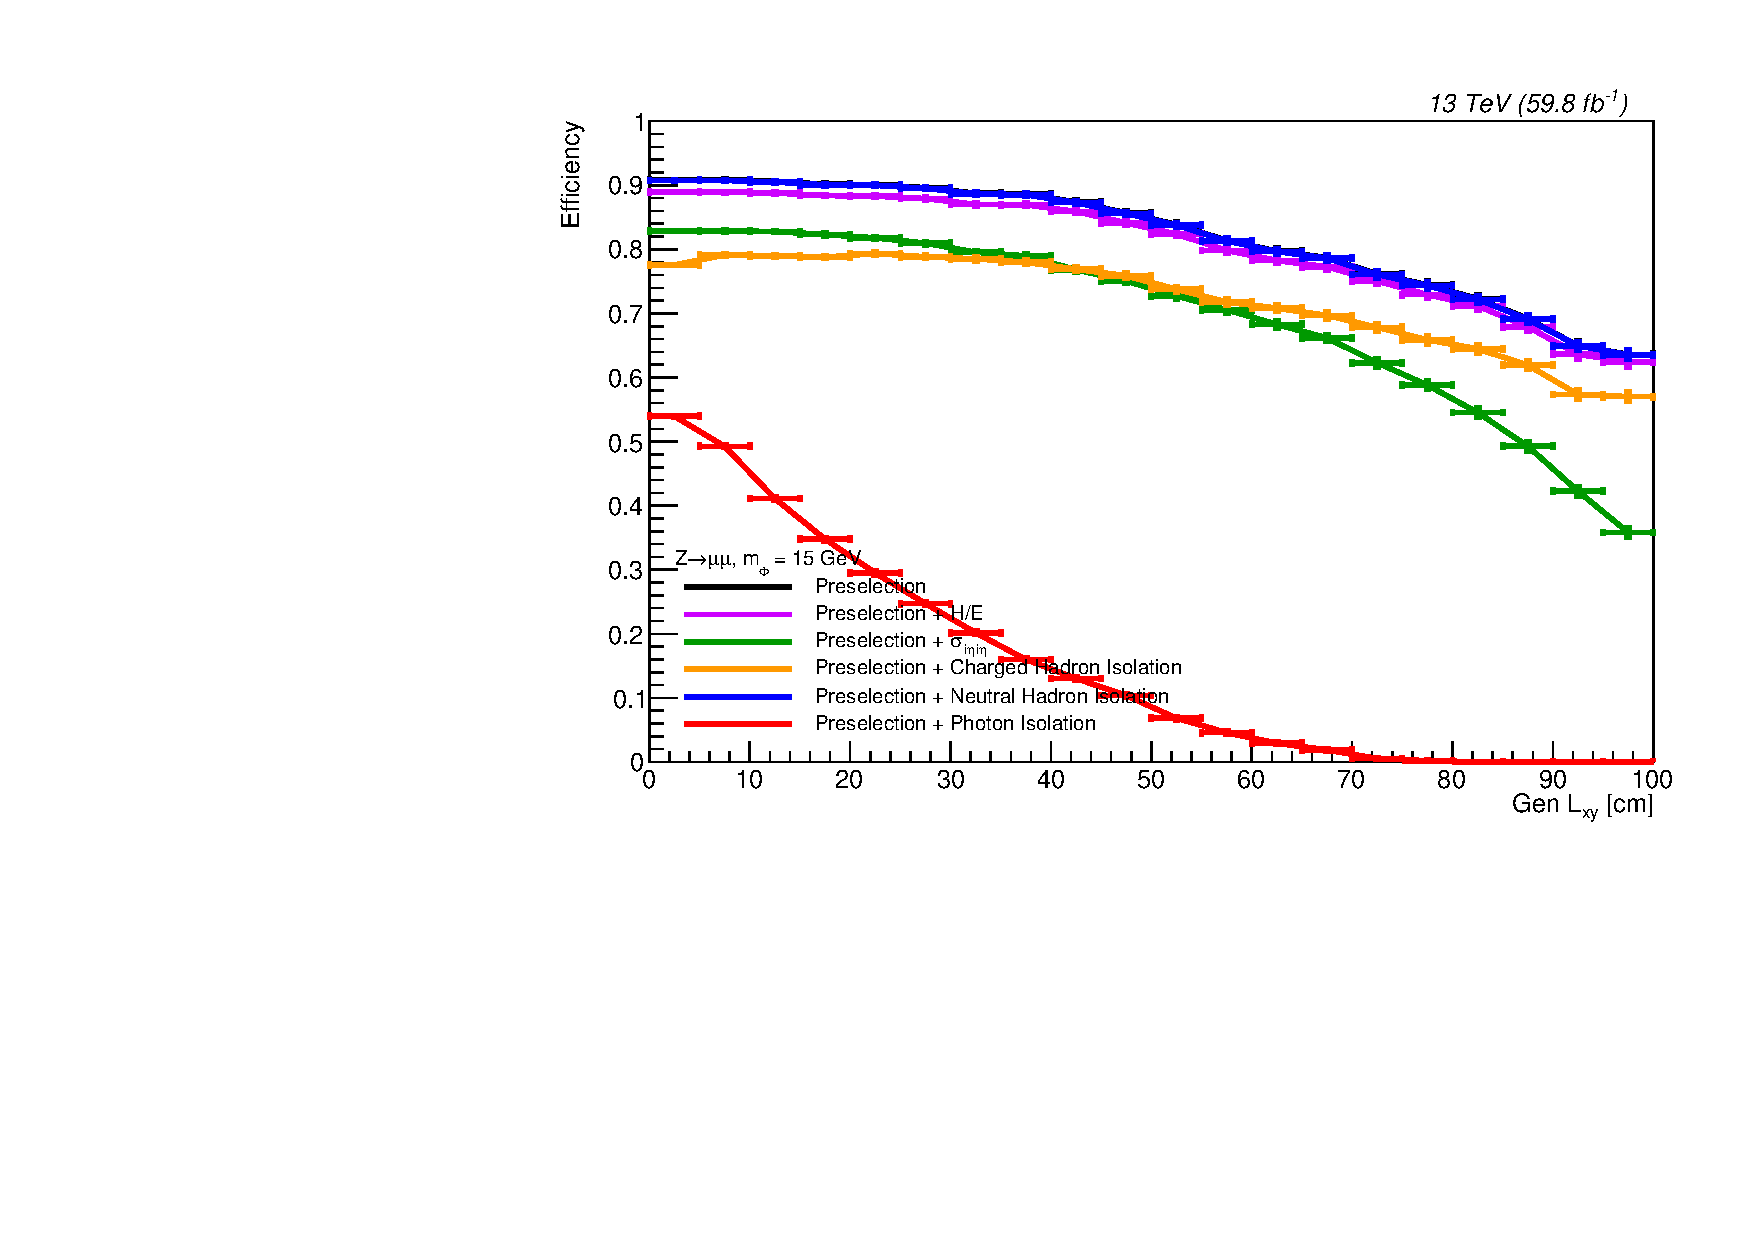
\includegraphics[width=\linewidth]{figs/05_analysis/cutBasedID_effVsLxy_Z_m15_cats_2018.pdf} &
		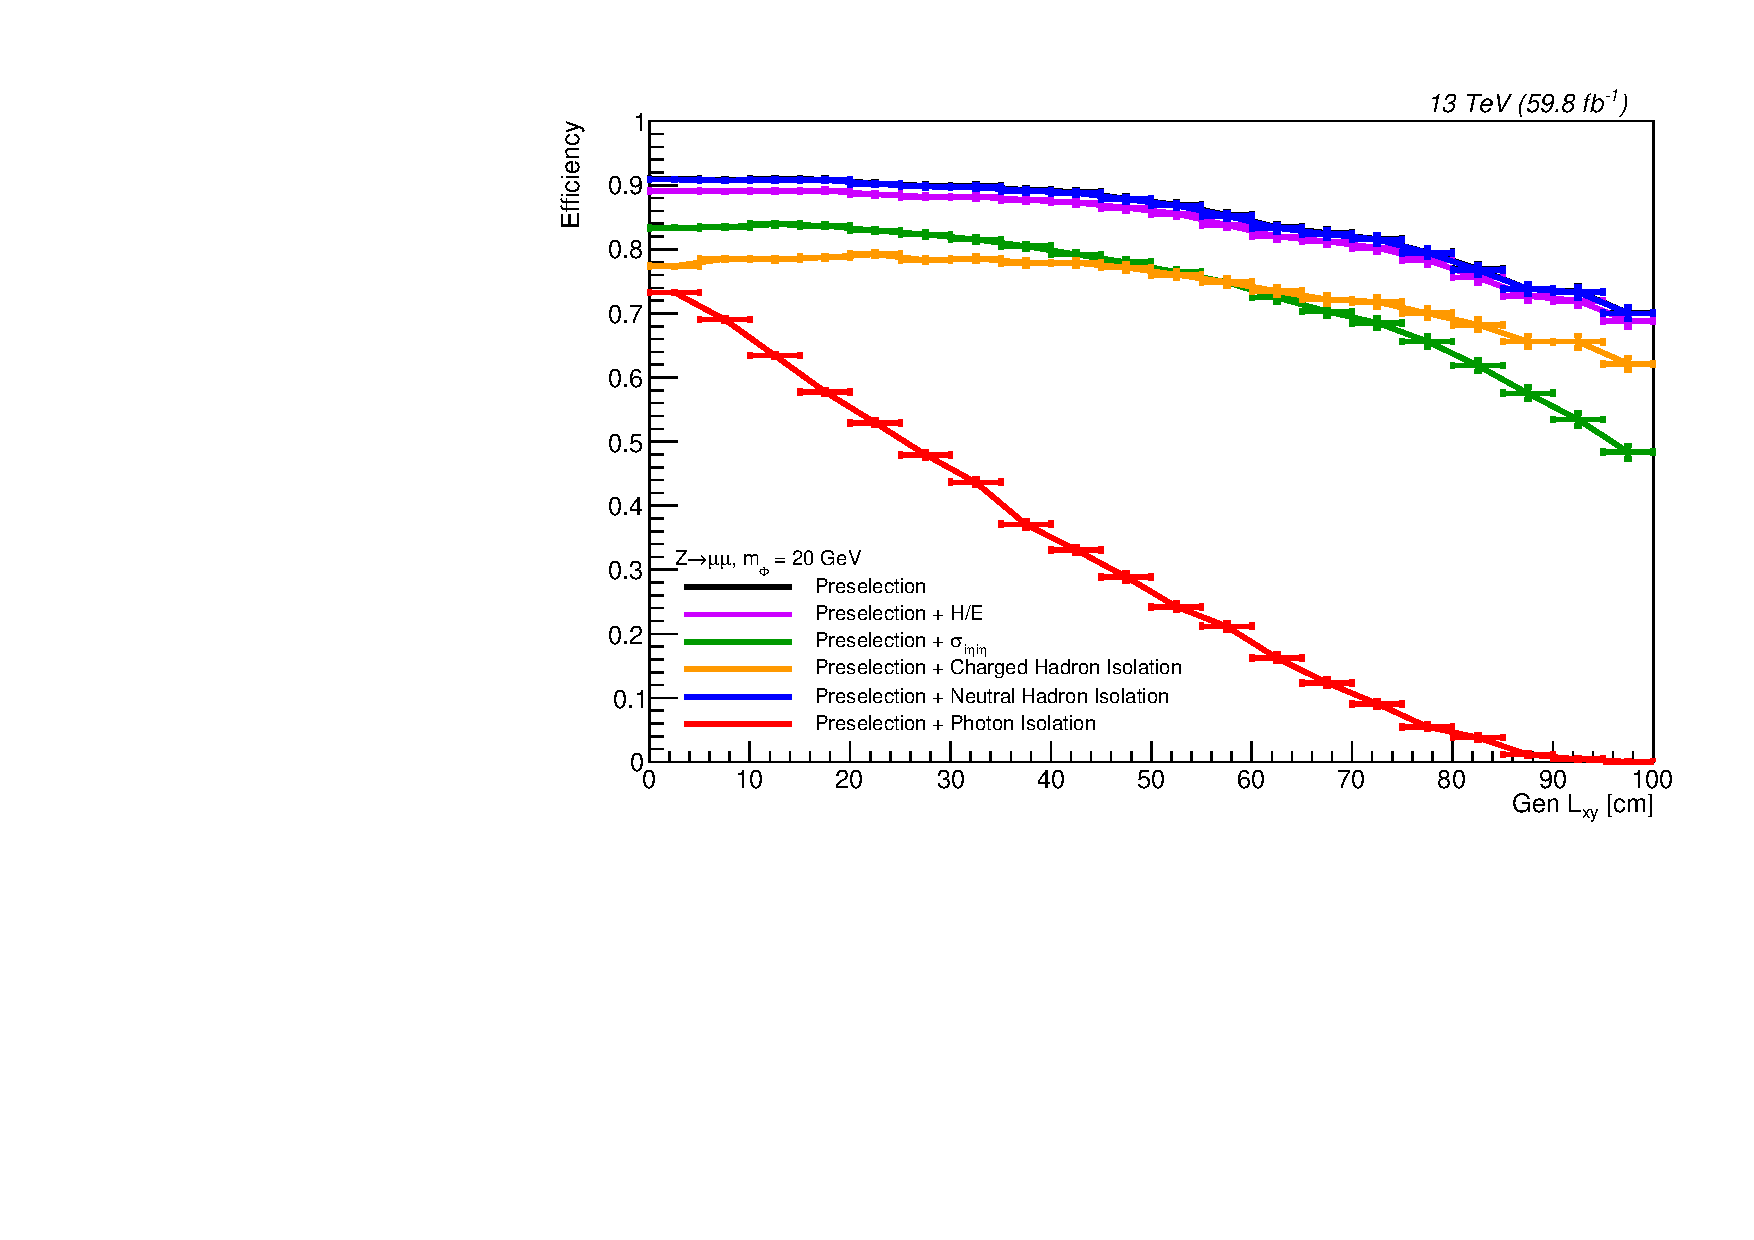
\includegraphics[width=\linewidth]{figs/05_analysis/cutBasedID_effVsLxy_Z_m20_cats_2018.pdf} &
		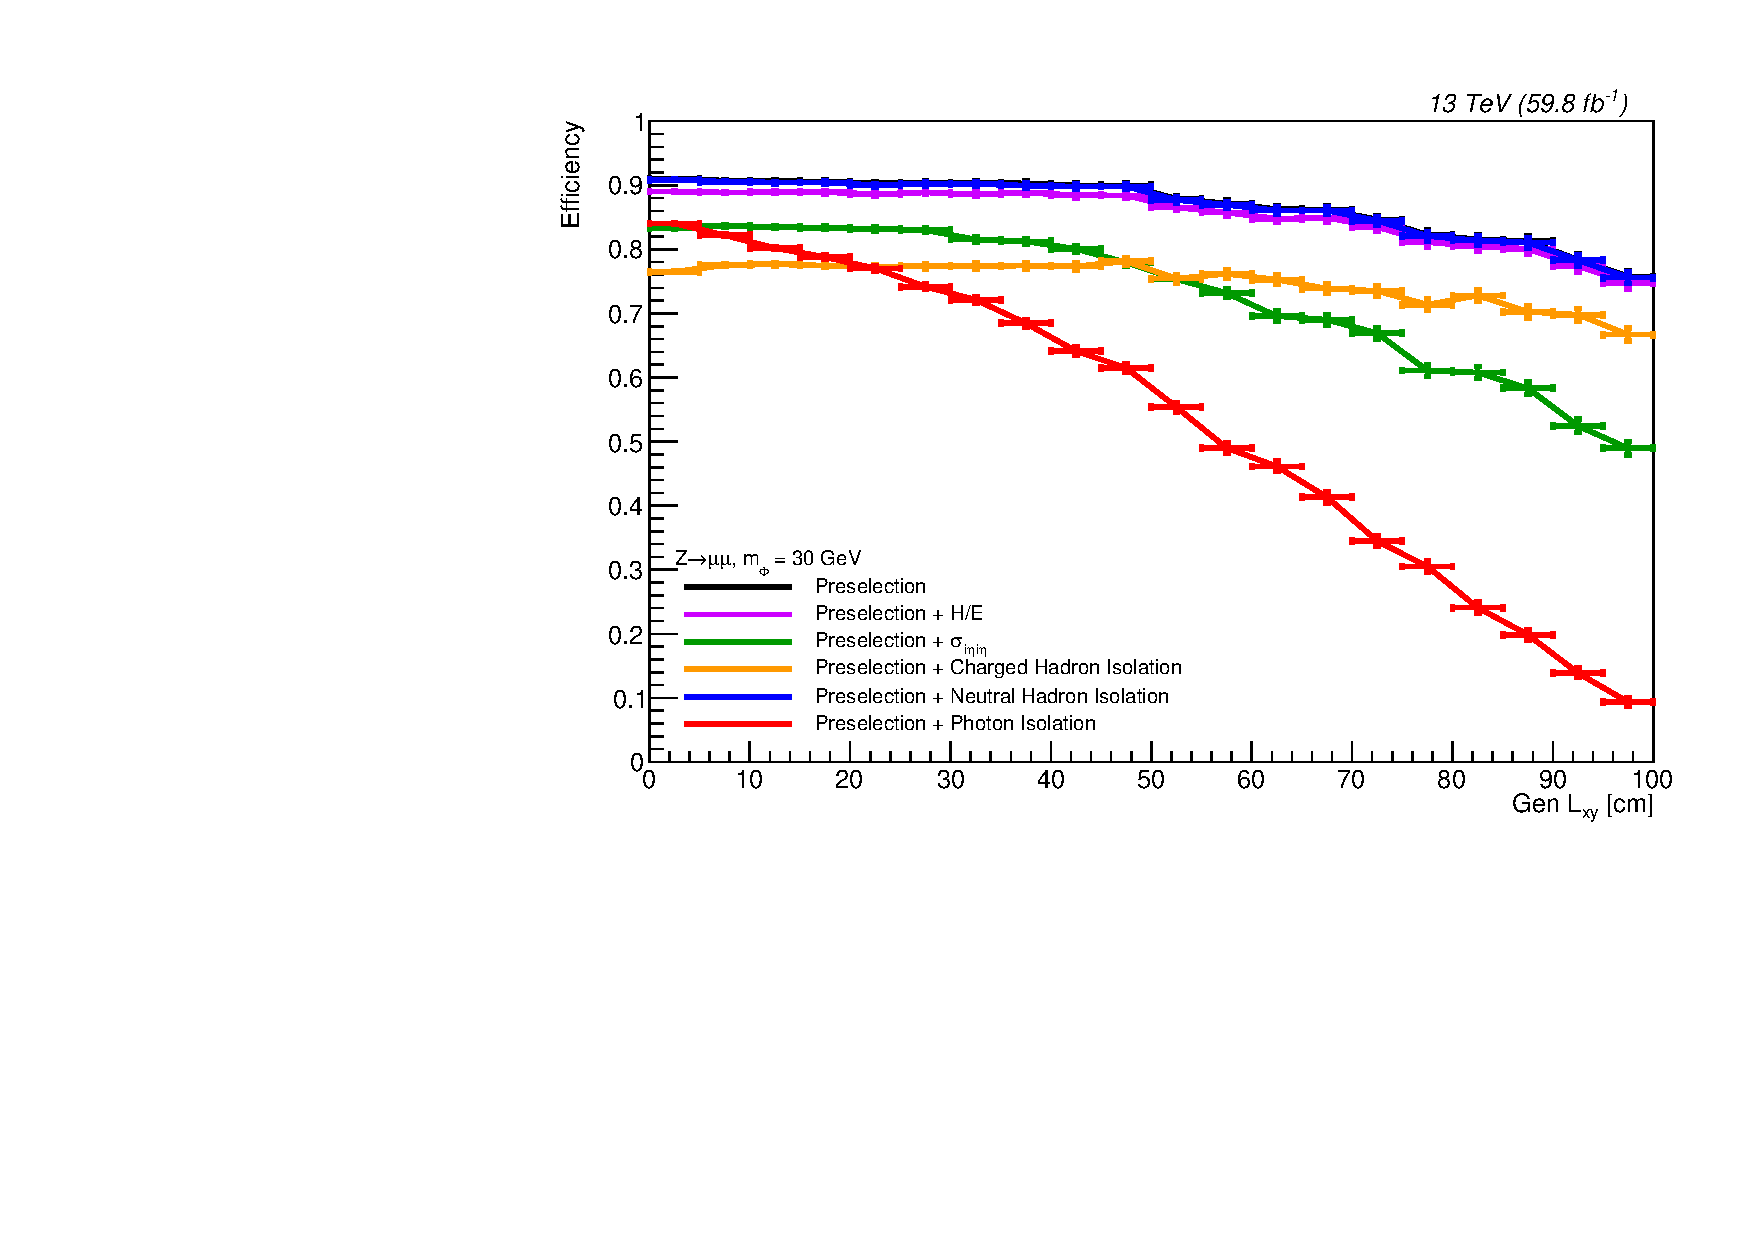
\includegraphics[width=\linewidth]{figs/05_analysis/cutBasedID_effVsLxy_Z_m30_cats_2018.pdf} \\
		$\mphi=40\GeV$ & $\mphi=50\GeV$ & $\mphi=55\GeV$ \\
		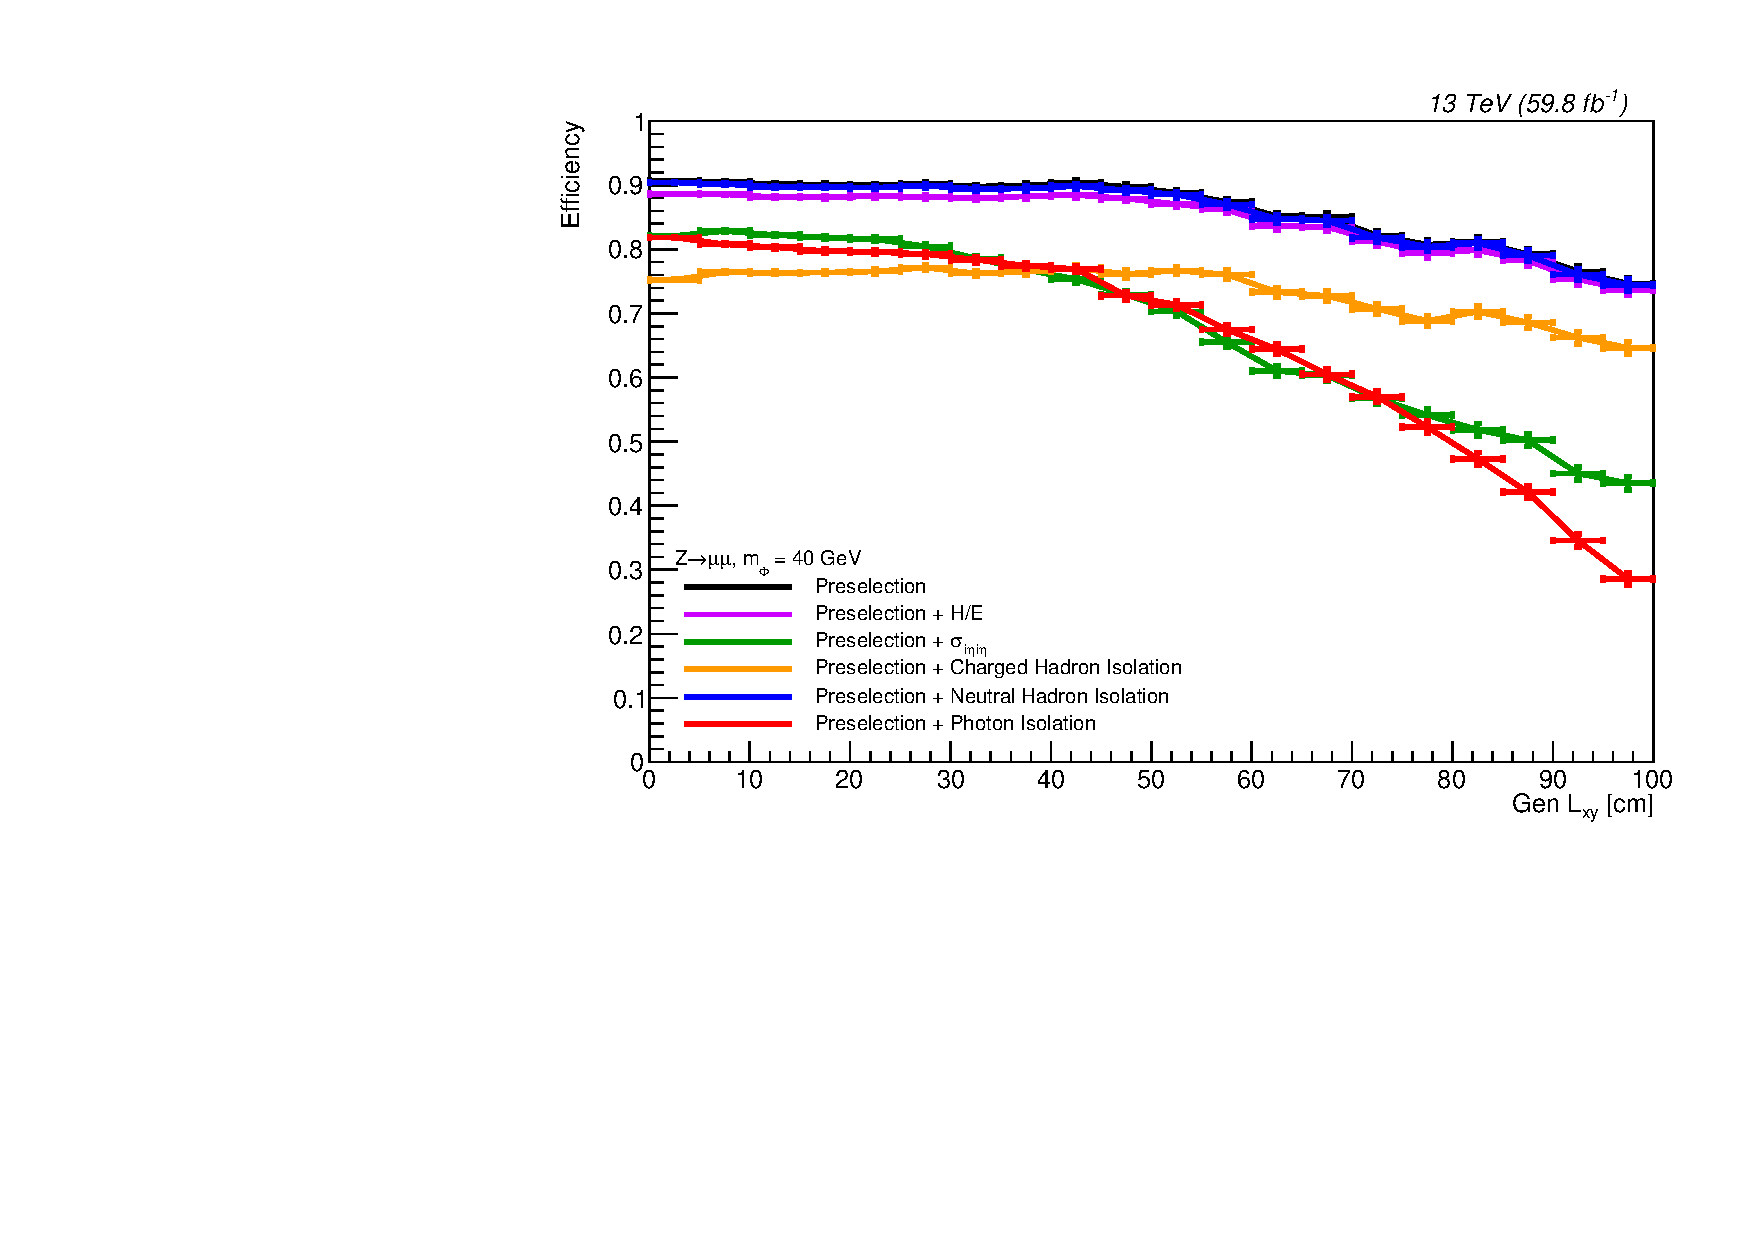
\includegraphics[width=\linewidth]{figs/05_analysis/cutBasedID_effVsLxy_Z_m40_cats_2018.pdf} &
		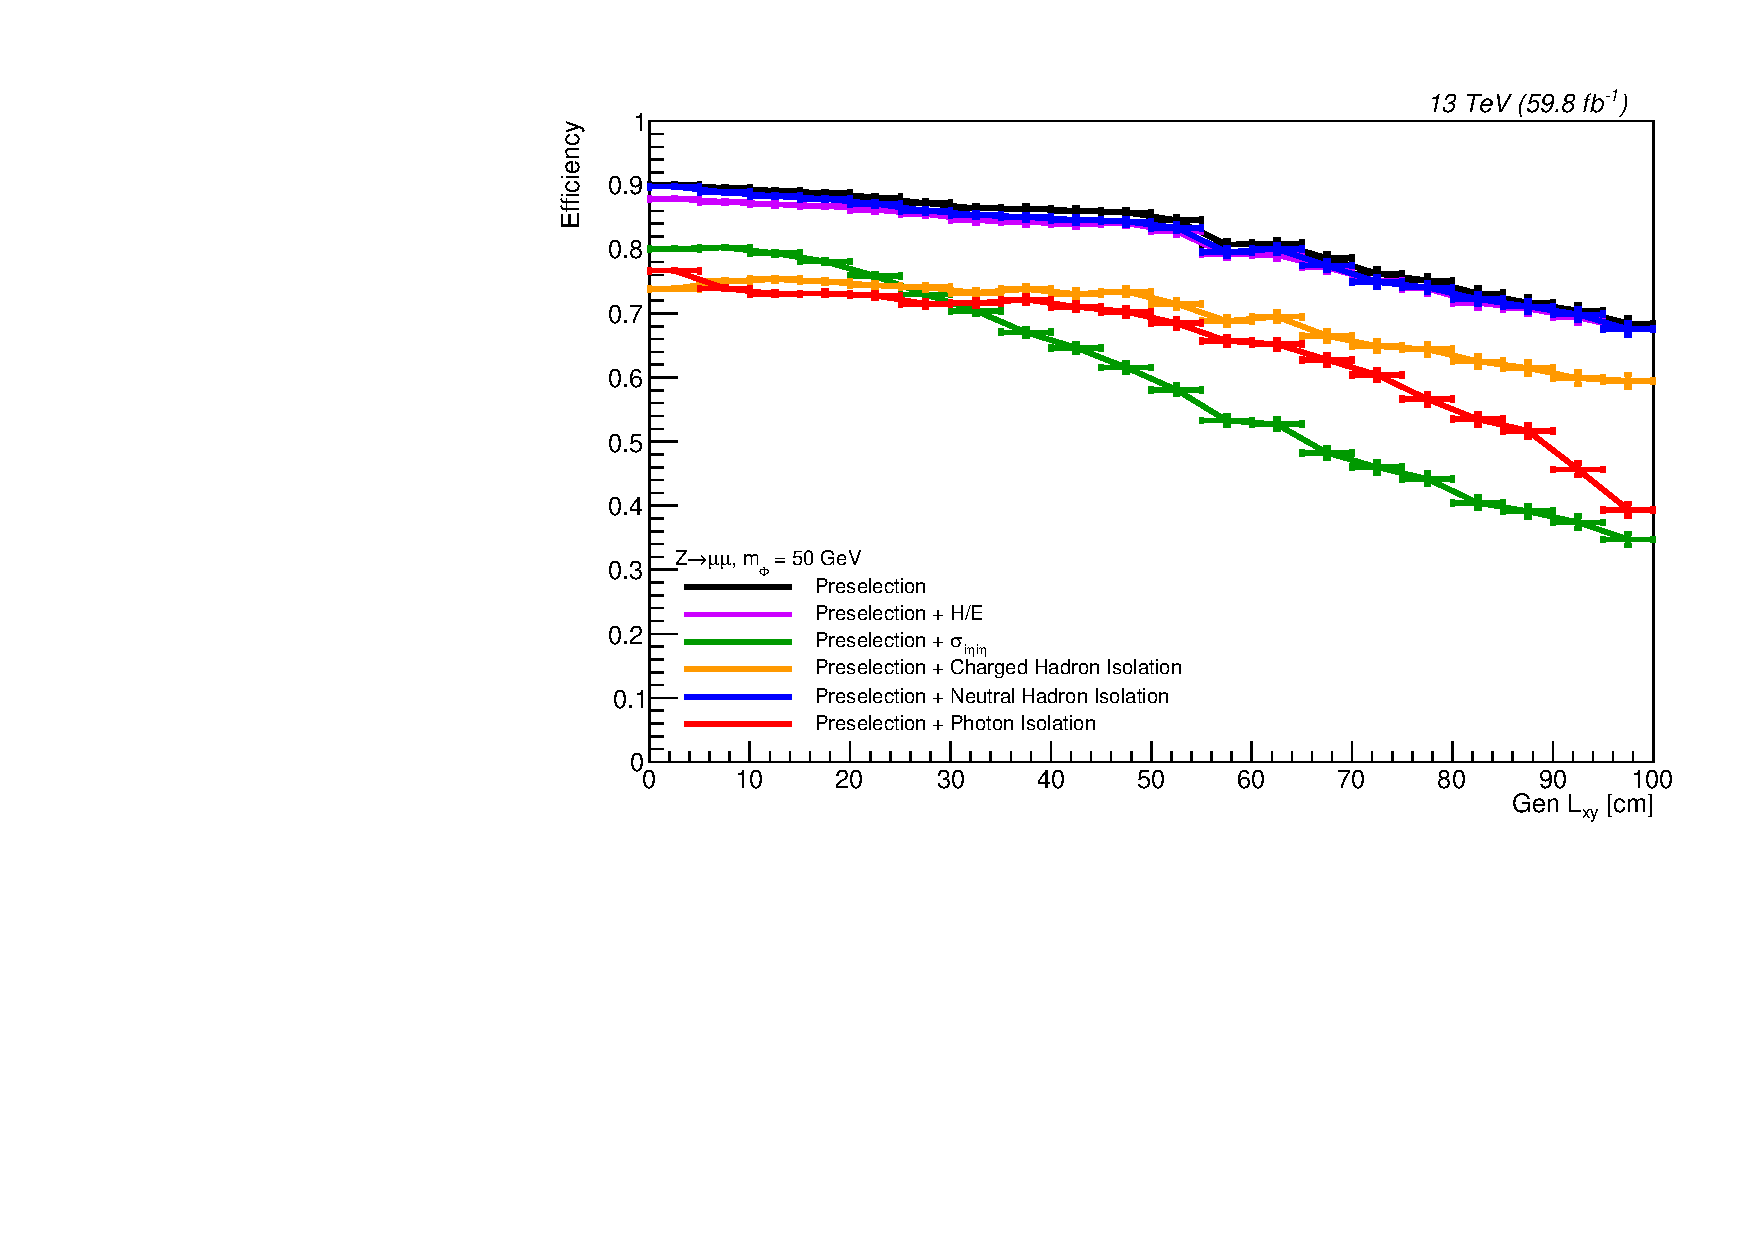
\includegraphics[width=\linewidth]{figs/05_analysis/cutBasedID_effVsLxy_Z_m50_cats_2018.pdf} &
		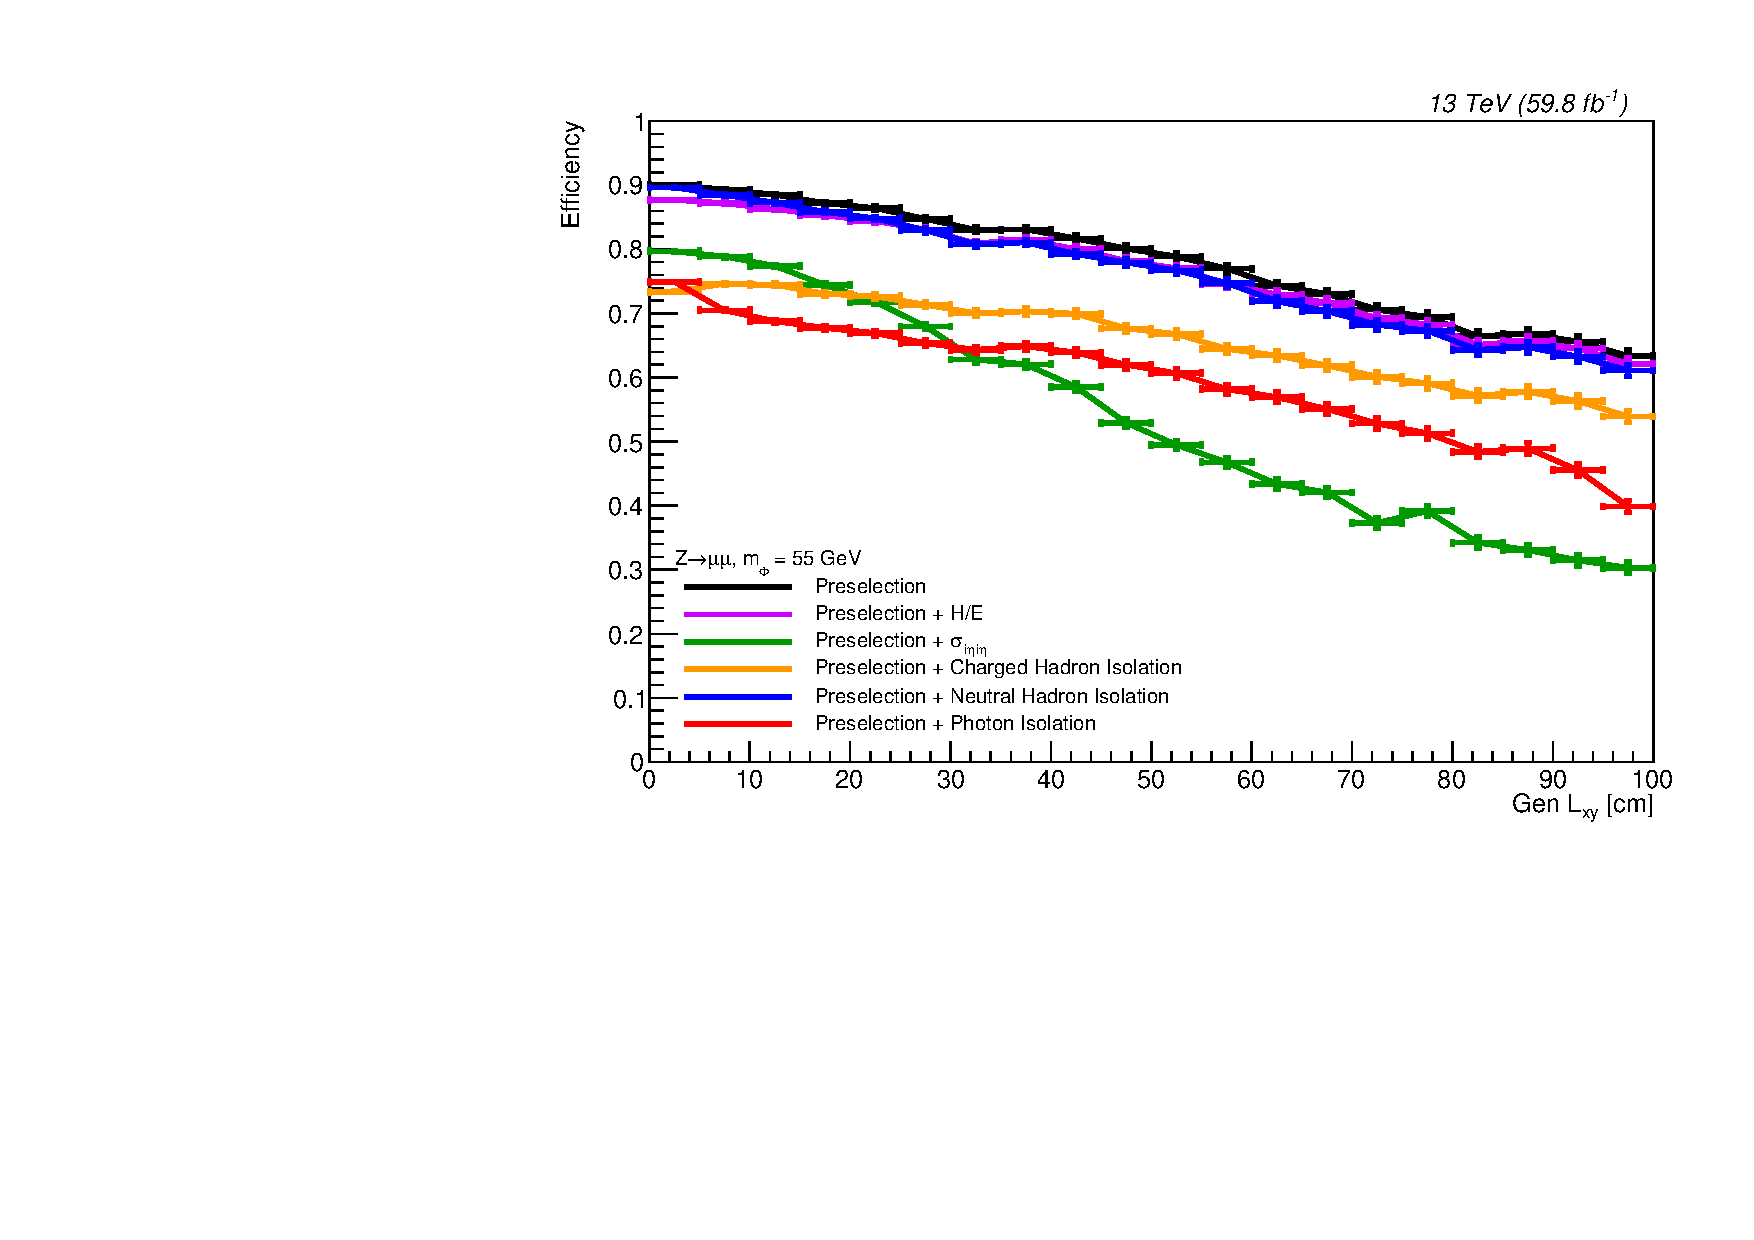
\includegraphics[width=\linewidth]{figs/05_analysis/cutBasedID_effVsLxy_Z_m55_cats_2018.pdf} \\
	\end{tabular}
	\caption[Efficiency for a photon pair to pass preselection versus generator level \lxy on ZH signal samples for all lifetimes in the $\PZ\to\PGm\PGm$ category.]{Efficiency for a photon pair to pass preselection versus generator level \lxy on ZH signal samples for all lifetimes in the $\PZ\to\PGm\PGm$ category. Denominator is all generator level photon pairs with each photon having $\pt>20\GeV$ that decay within the geometric acceptance of the ECAL. The numerator requires two matching ($\Delta r<0.3$, energy within 50\% of gen photon) reconstructed photons passing preselection criteria. Cut based ID is applied on top of preselection, showing that the dominant inefficiencies at high \lxy are due to $I_\gamma$ and $\sigma_{i\eta i\eta}$.}
	\label{fig:Photon_cutBased}
\end{figure}

\subsection{Signal Region Definitions} \label{sec:ana_signalregion}
$\Phi$ candidates are reconstructed from events with at least two photons passing preselection criteria. If there are only two photons that pass preselection, the diphotons are chosen as a possible $\Phi$ candidate. If more than two photons pass this criteria, the photons will be subject to pairing criteria for every candidate mass of the $\Phi$. This pairing process is designed to maximize pairing efficiency, as without pointing capabilities there is no consistent, robust way to determine whether signal photons originated from the same $\Phi$, while also minimizing the bias introduced through the pairing criteria. For each candidate mass, photon pairs are chosen as follows:
\begin{itemize}
	\item The pair with an energetically allowed decay is chosen (i.e. there is a physical solution to equation~\ref{eq:me1e2theta})
	\item If multiple pairs have allowed decays, the pair with more photons passing cut based ID is chosen
	\item If multiple pairs use the same number of photons passing ID, the pair with the largest prompt invariant mass \mgg is chosen
	\item If multiple pairs have the same \mgg, the pair with the highest \ptgg is chosen
\end{itemize}
For convention, the leading higher \pt photon is referred to as $\gamma_1$ while the sub-leading lower \pt photon is referred to as $\gamma_2$.

The signal region is defined by the presence of one \PZ candidate and at least one $\Phi$ candidate composed of two ID'd photons. Events are categorized based on the lepton flavor of the Z decay to either muons or electrons. For each signal region category, an anti-ID control region is utilized for background estimation. These categories are defined identically to the signal region but require the $\Phi$ candidate to use one photon passing the loose cut based ID and one photon failing loose cut based ID defined in table~\ref{tab:photonID}.

To compare data to simulated background, the dilepton mass \mll is plotted in all categories for the signal region and anti-ID control region in figures~\ref{fig:zmass_preselection_med}$\,$-$\,$\ref{fig:zmass_preselection_tight}. These distributions are made agnostic to the vertex calculation and have no cuts on diphoton \lxy. The results show moderate agreement in the anti-ID control region and limited statistical power for simulated events in the ID signal region. Comparisons show an excess of events below $90\GeV$ due to the presence of final state radiation.

\begin{figure}[htb!]
	\centering
	\begin{tabular}{>{\centering\arraybackslash}m{0.32\linewidth} >{\centering\arraybackslash}m{0.32\linewidth} >{\centering\arraybackslash}m{0.32\linewidth}}
		2018 $\PZ\to\PGm\PGm$ & 2017 $\PZ\to\PGm\PGm$ & 2016 $\PZ\to\PGm\PGm$\\
		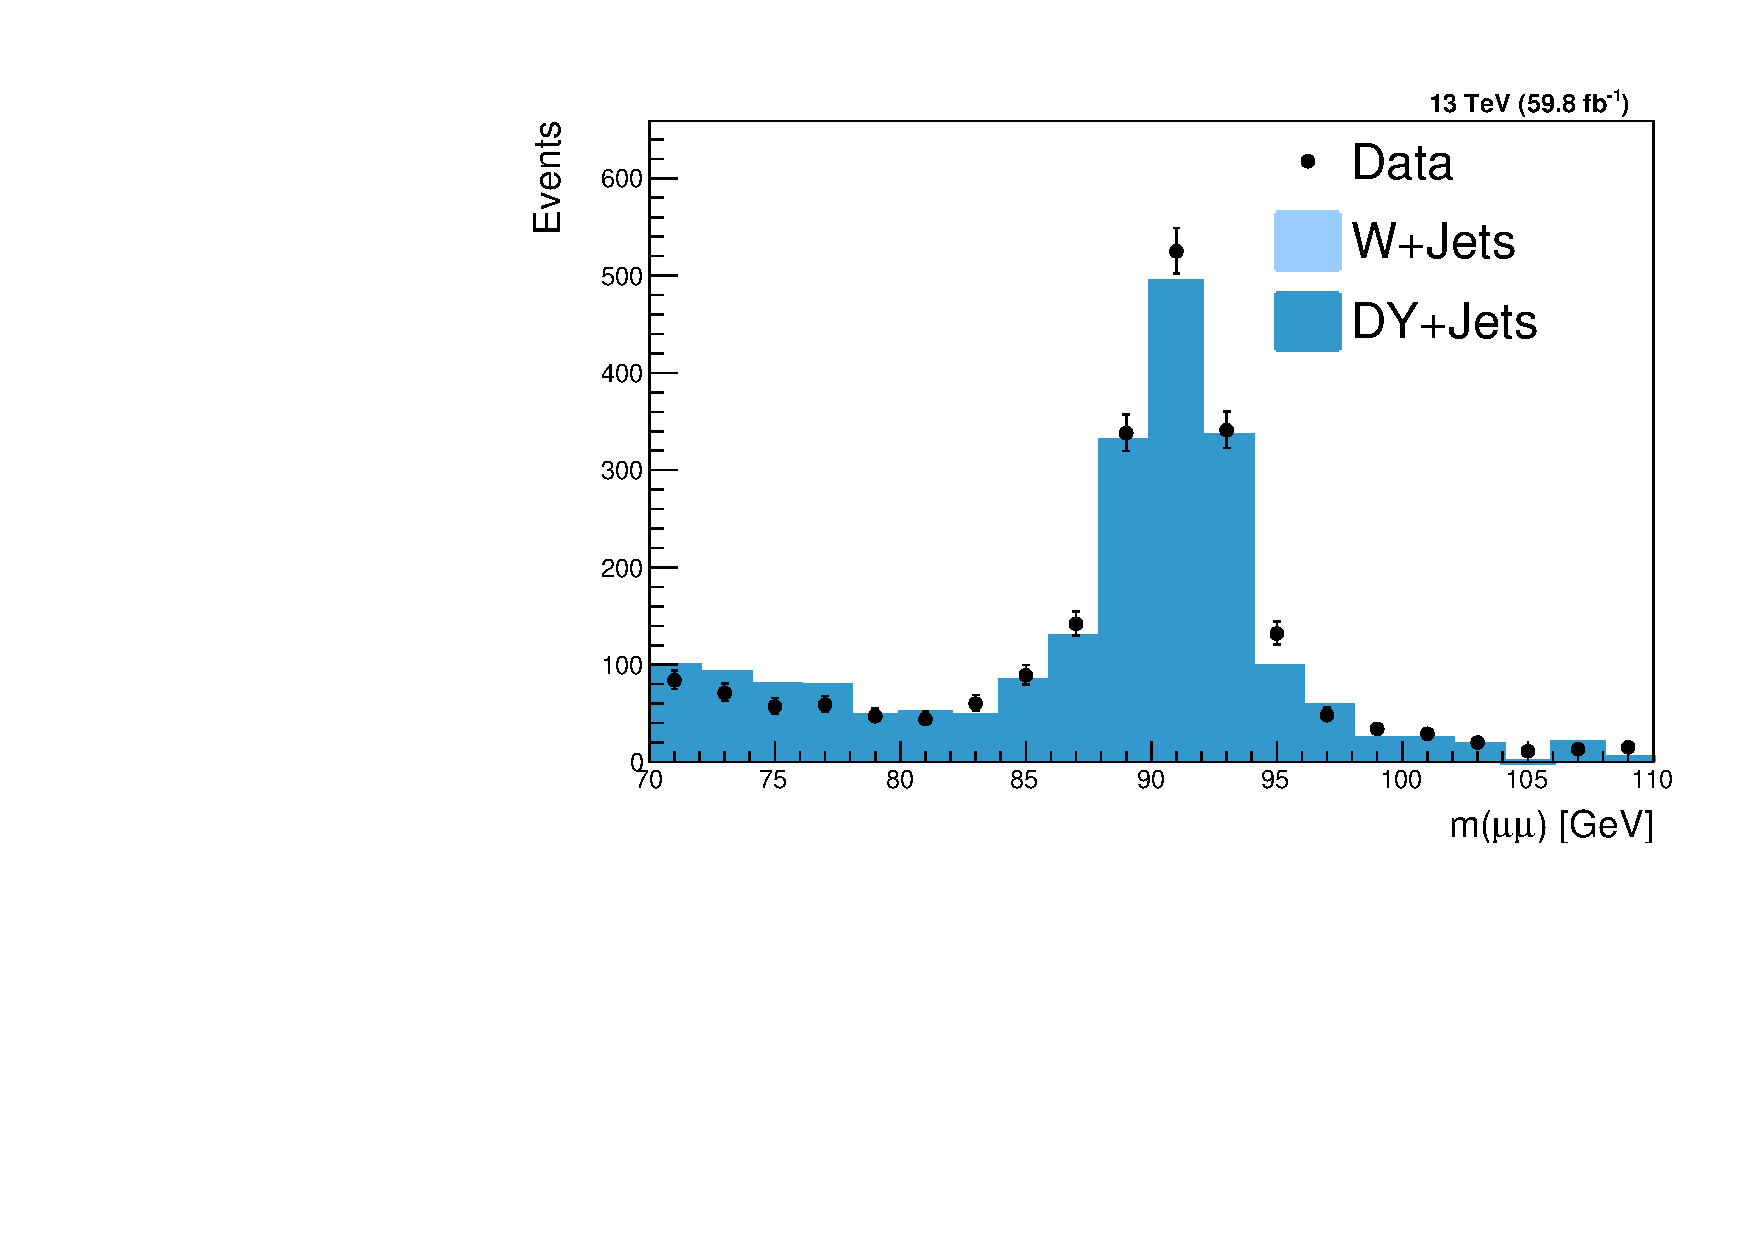
\includegraphics[width=\linewidth]{figs/05_analysis/2018_ZX_Z_mass_MU_preselection_med.pdf} &
		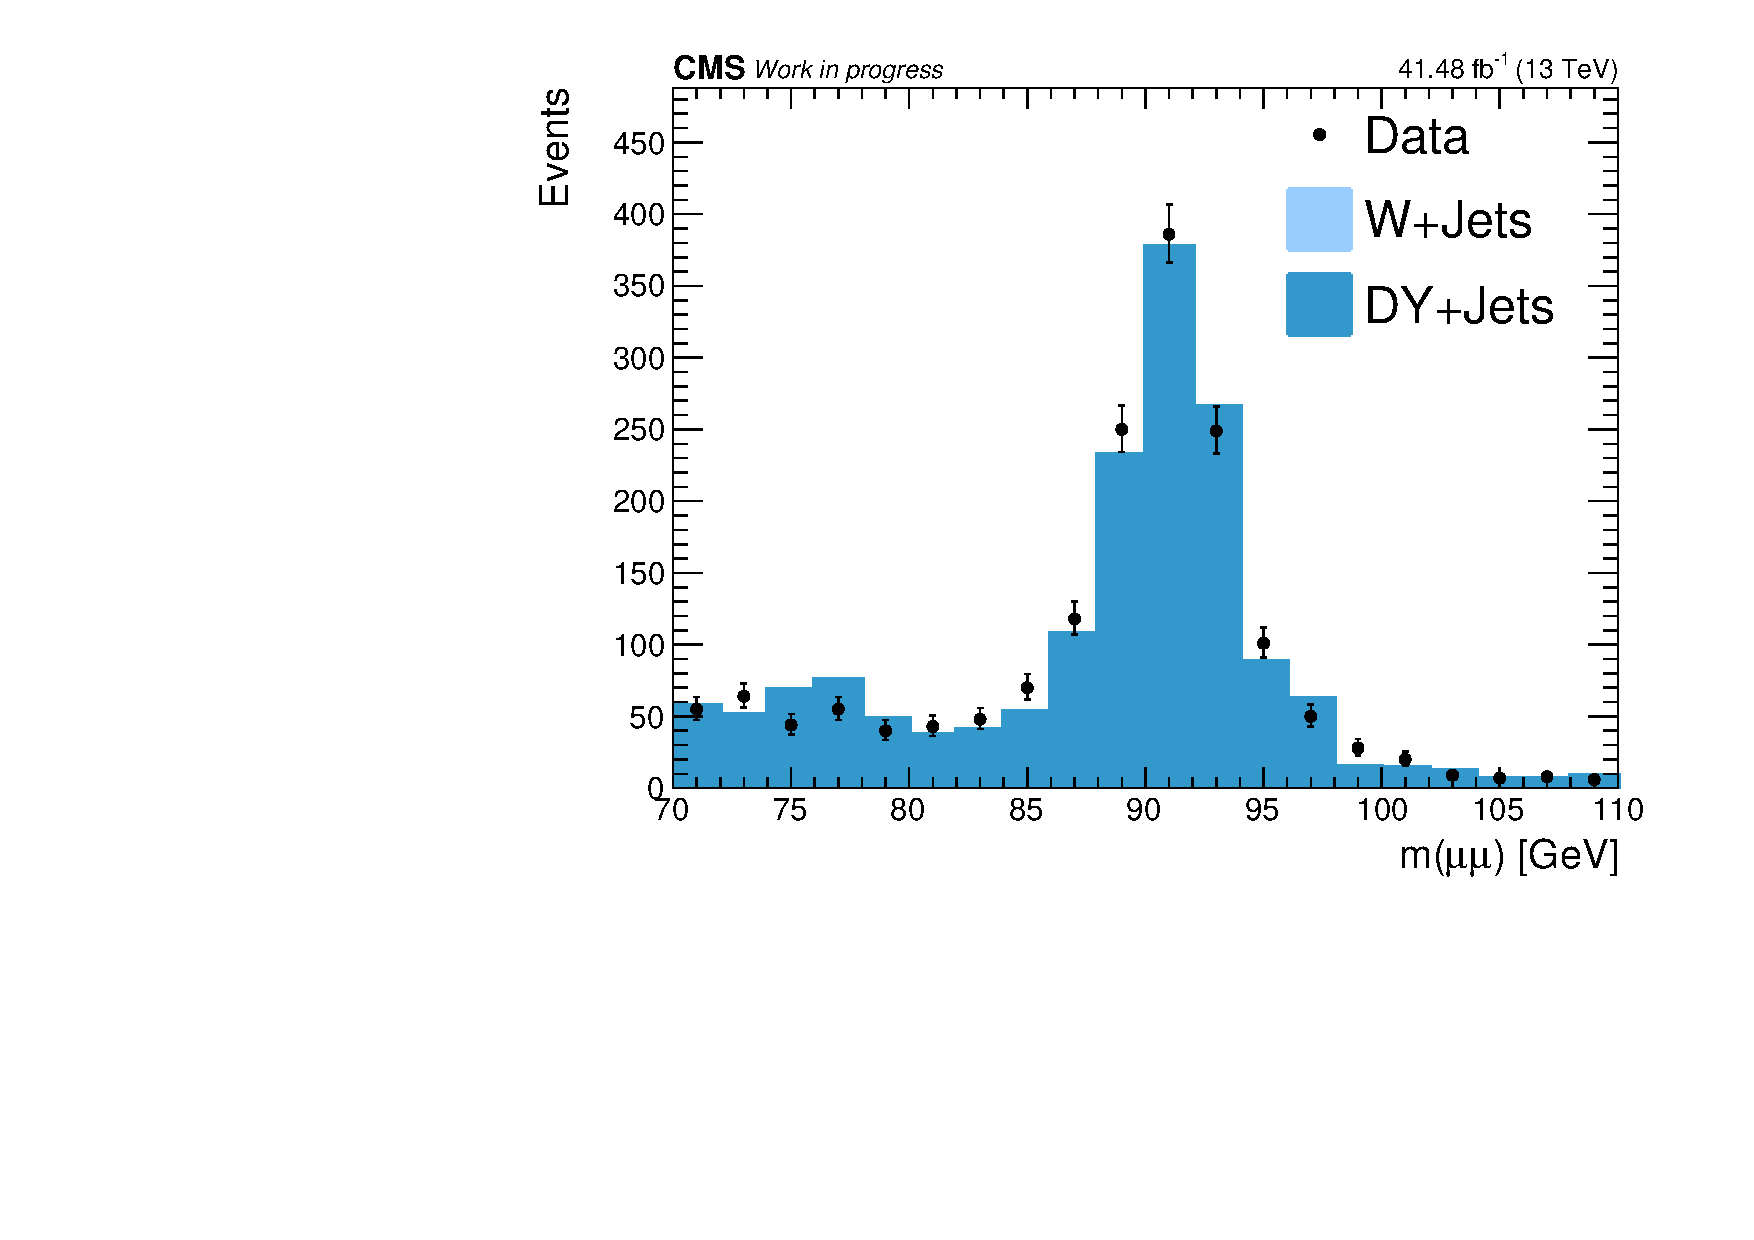
\includegraphics[width=\linewidth]{figs/05_analysis/2017_ZX_Z_mass_MU_preselection_med.pdf} &
		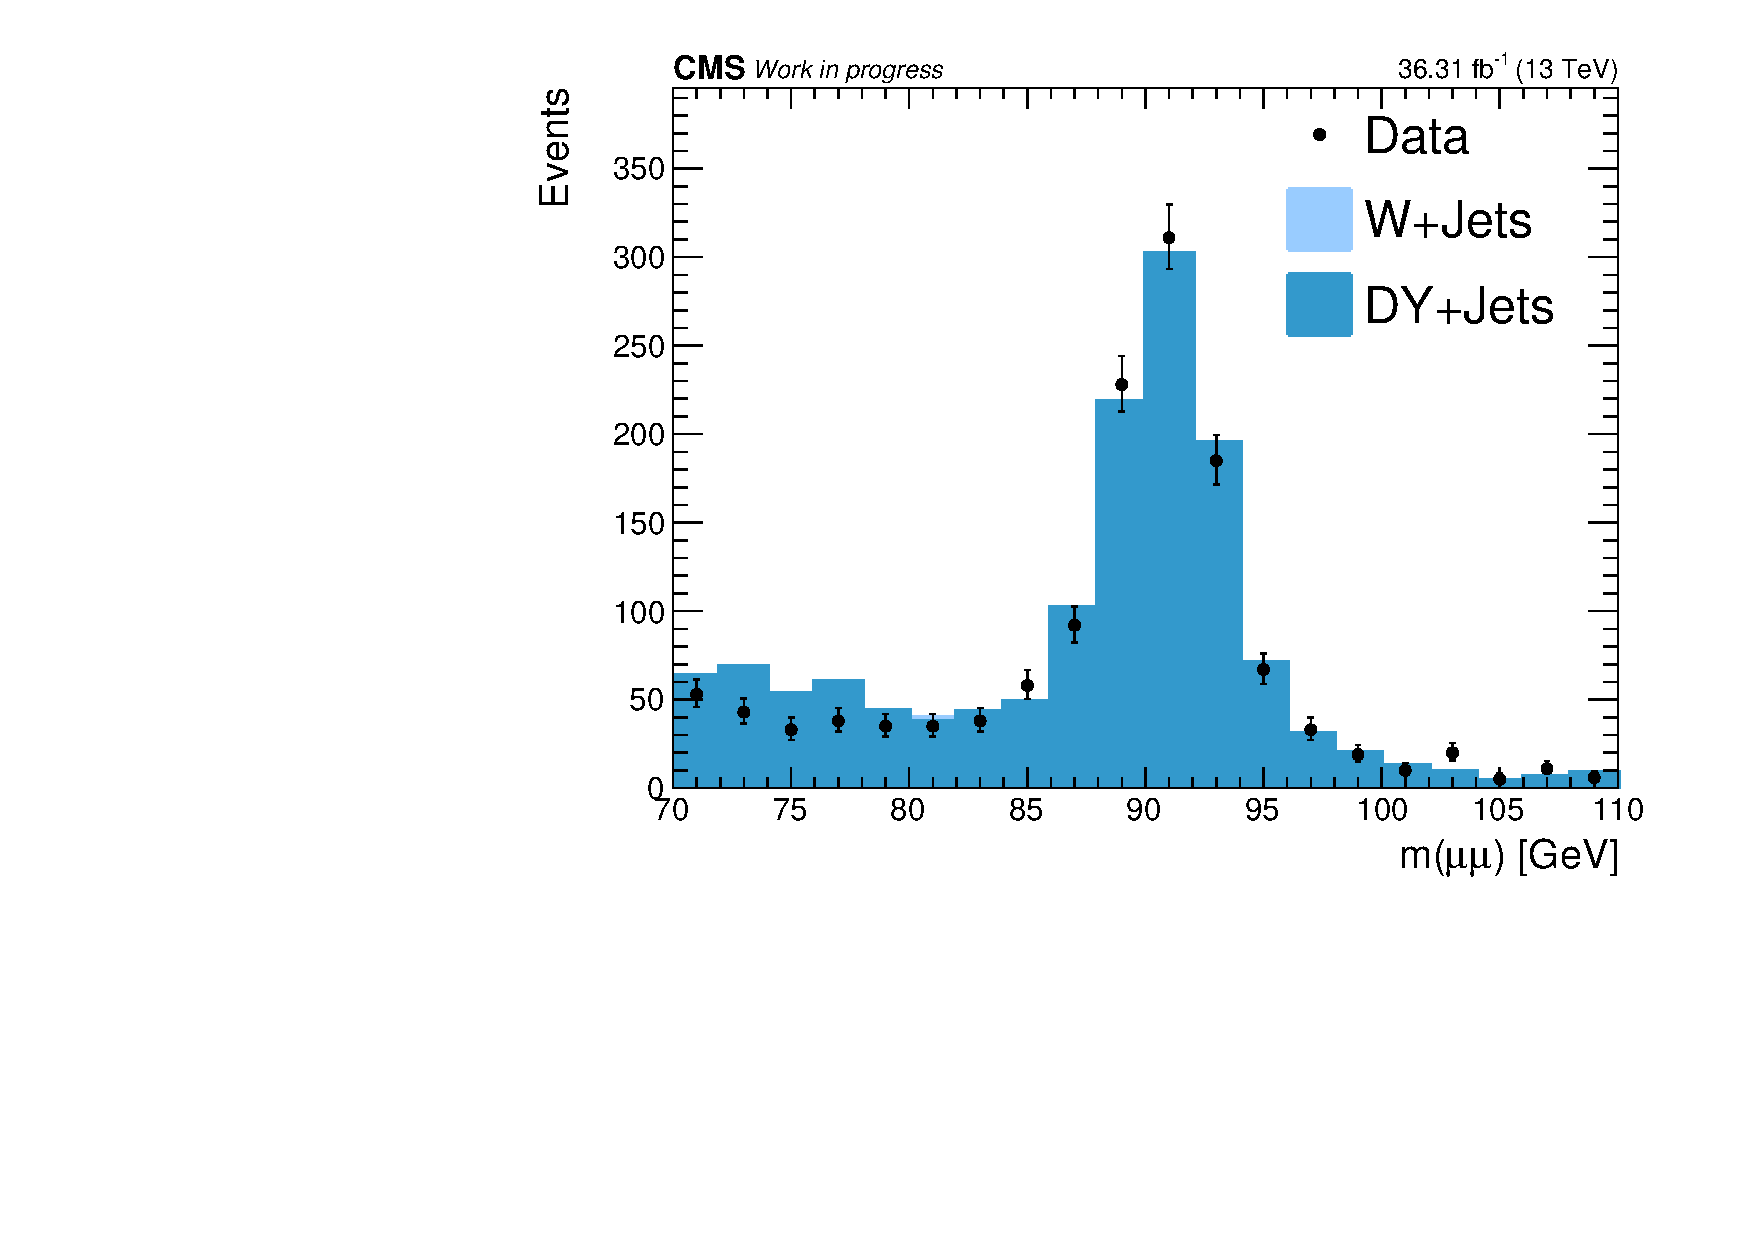
\includegraphics[width=\linewidth]{figs/05_analysis/2016_ZX_Z_mass_MU_preselection_med.pdf} \\
		2018 $\PZ\to\Pe\Pe$ & 2017 $\PZ\to\Pe\Pe$ & 2016 $\PZ\to\Pe\Pe$\\
		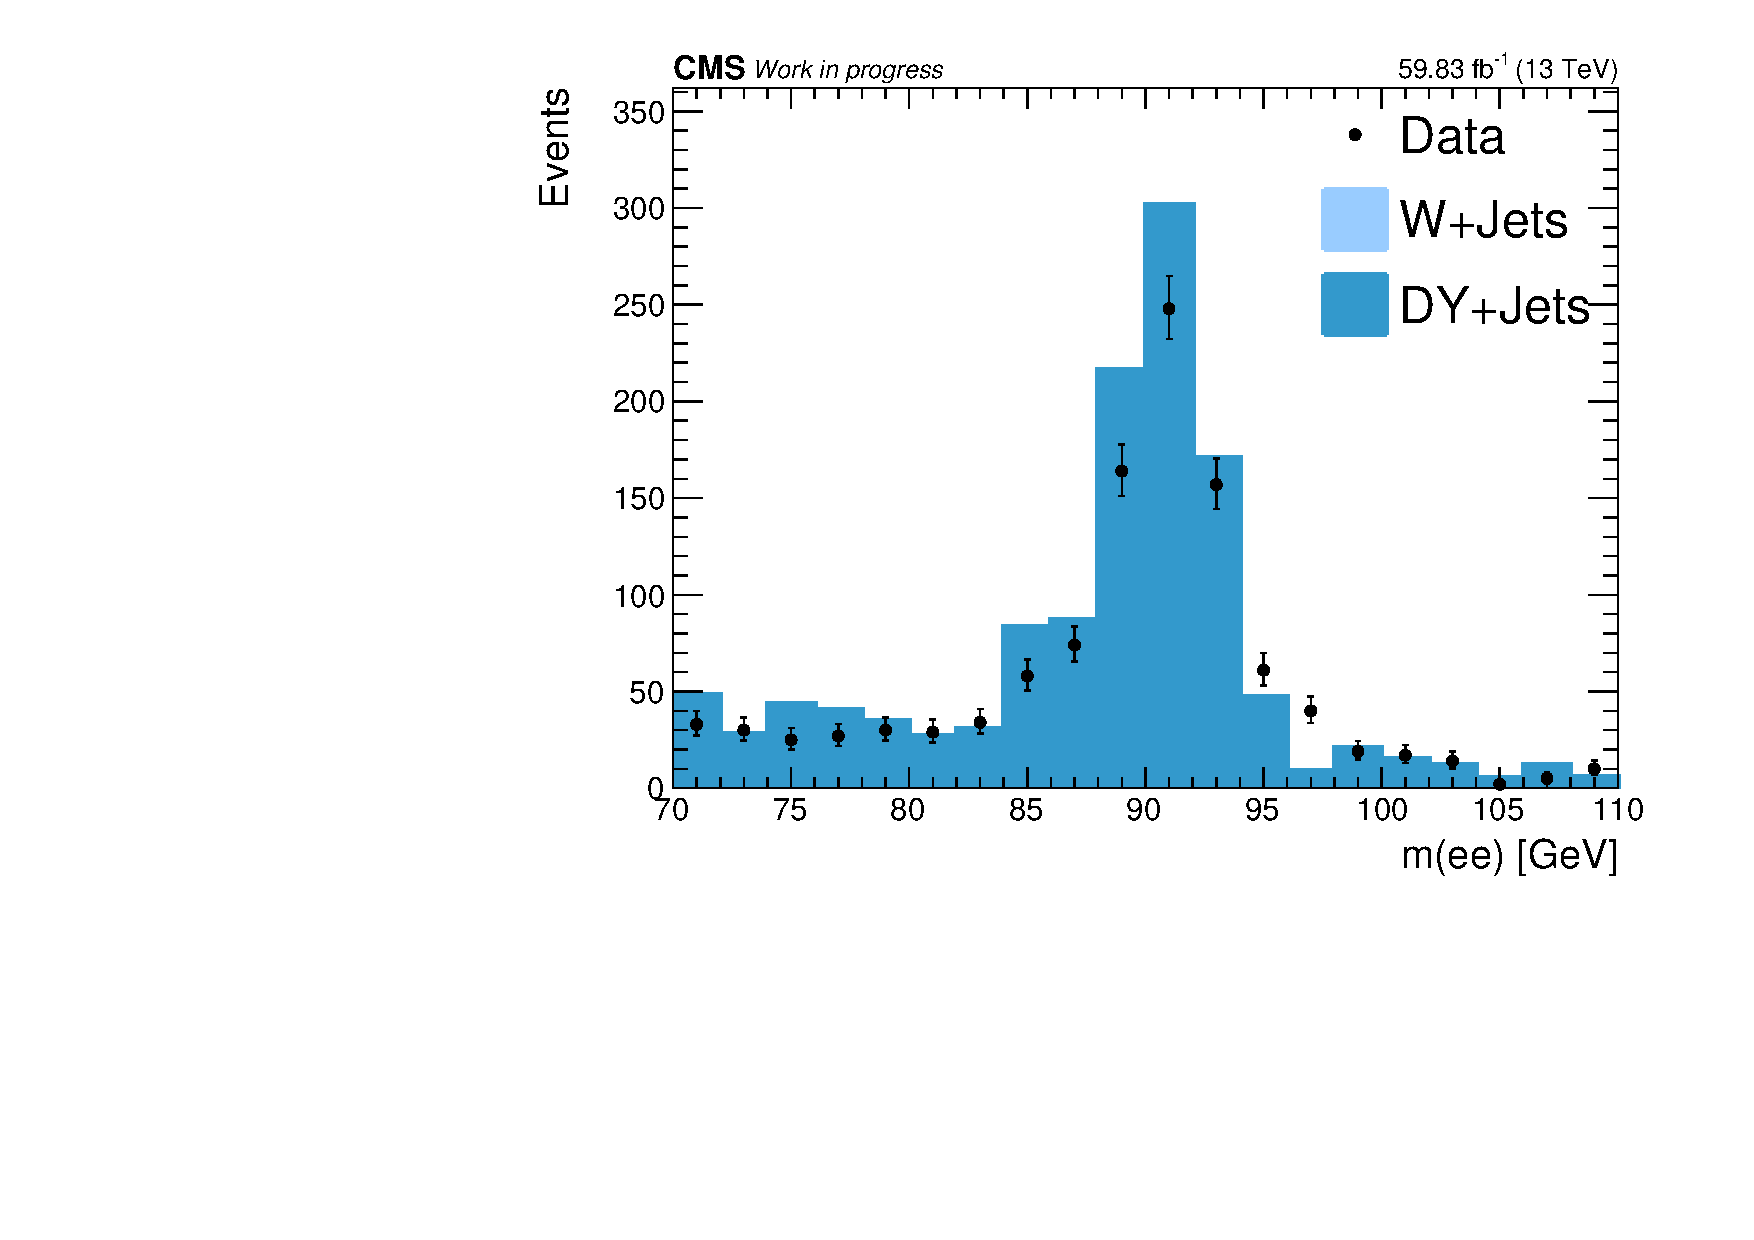
\includegraphics[width=\linewidth]{figs/05_analysis/2018_ZX_Z_mass_ELE_preselection_med.pdf} &
		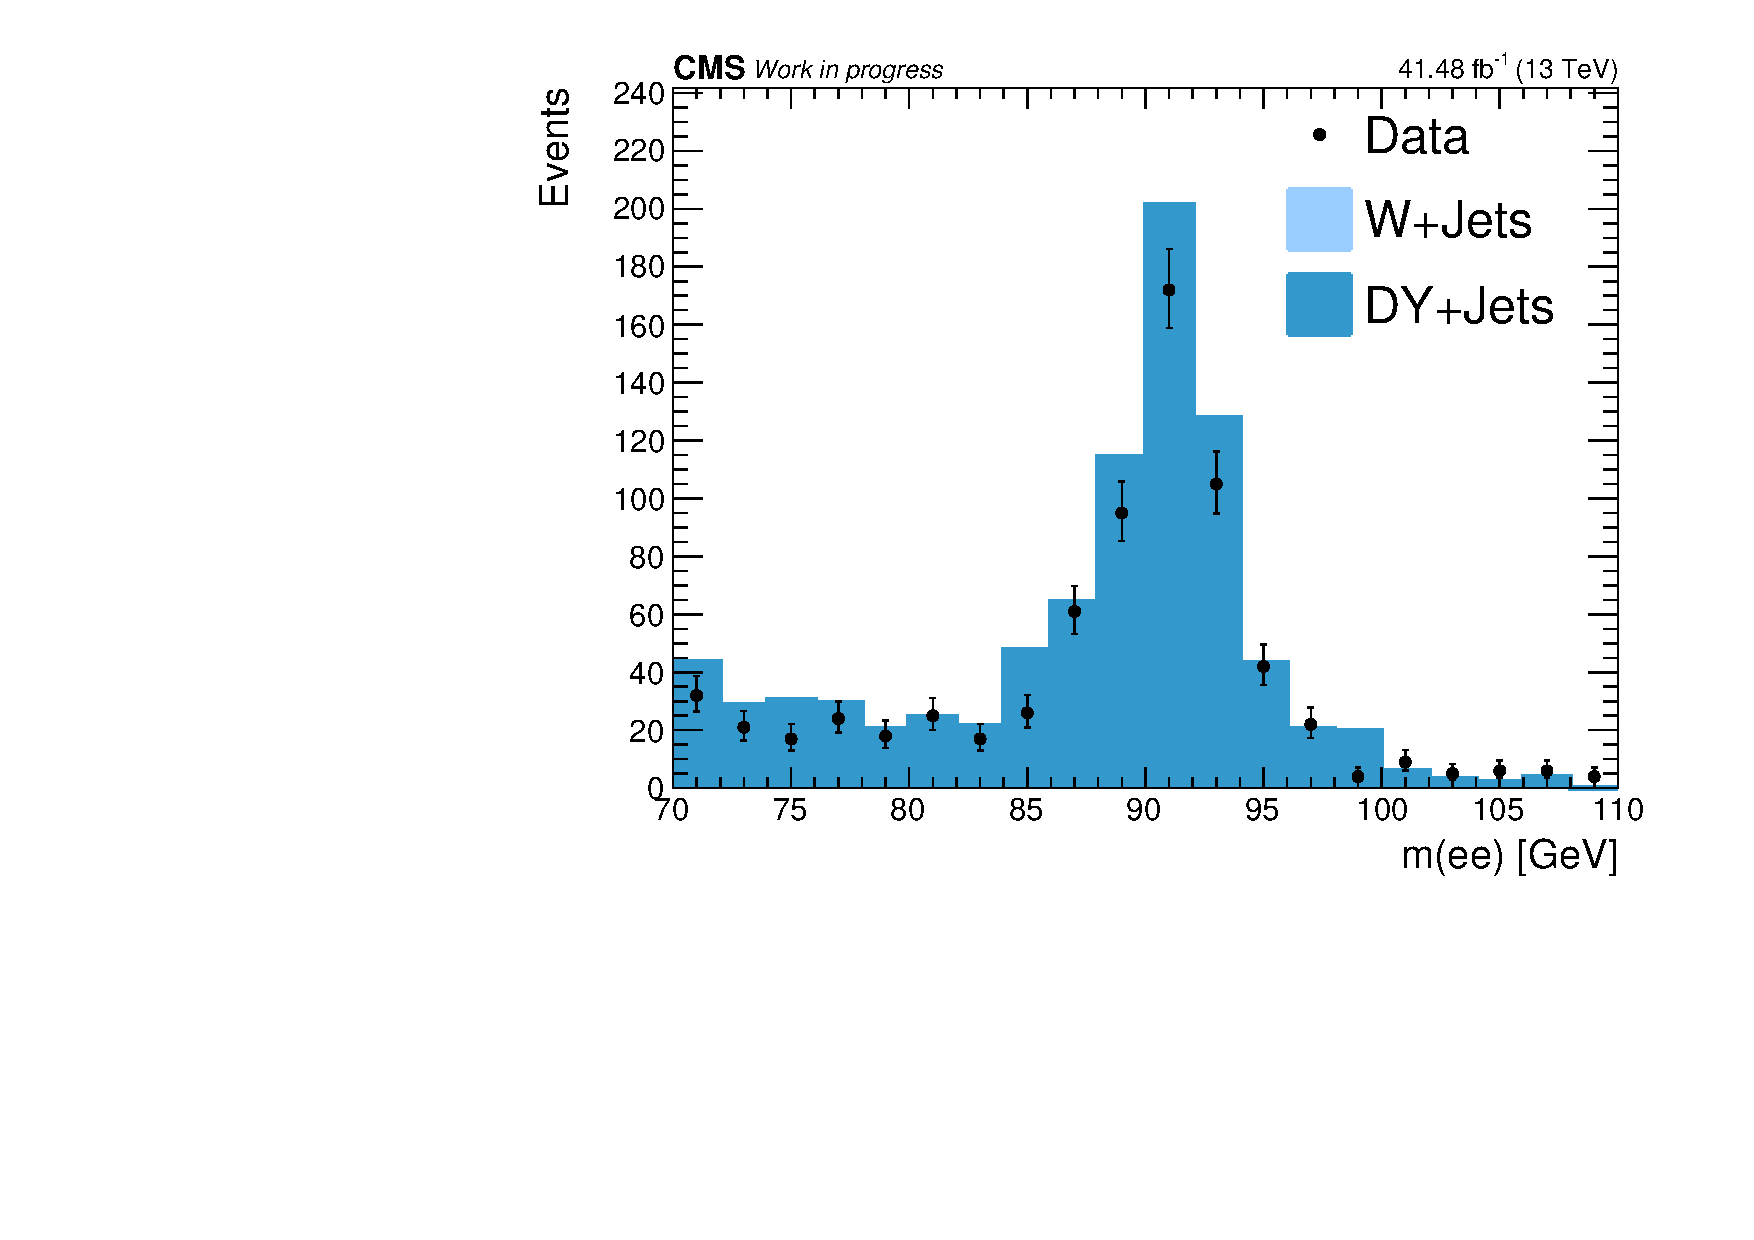
\includegraphics[width=\linewidth]{figs/05_analysis/2017_ZX_Z_mass_ELE_preselection_med.pdf} &
		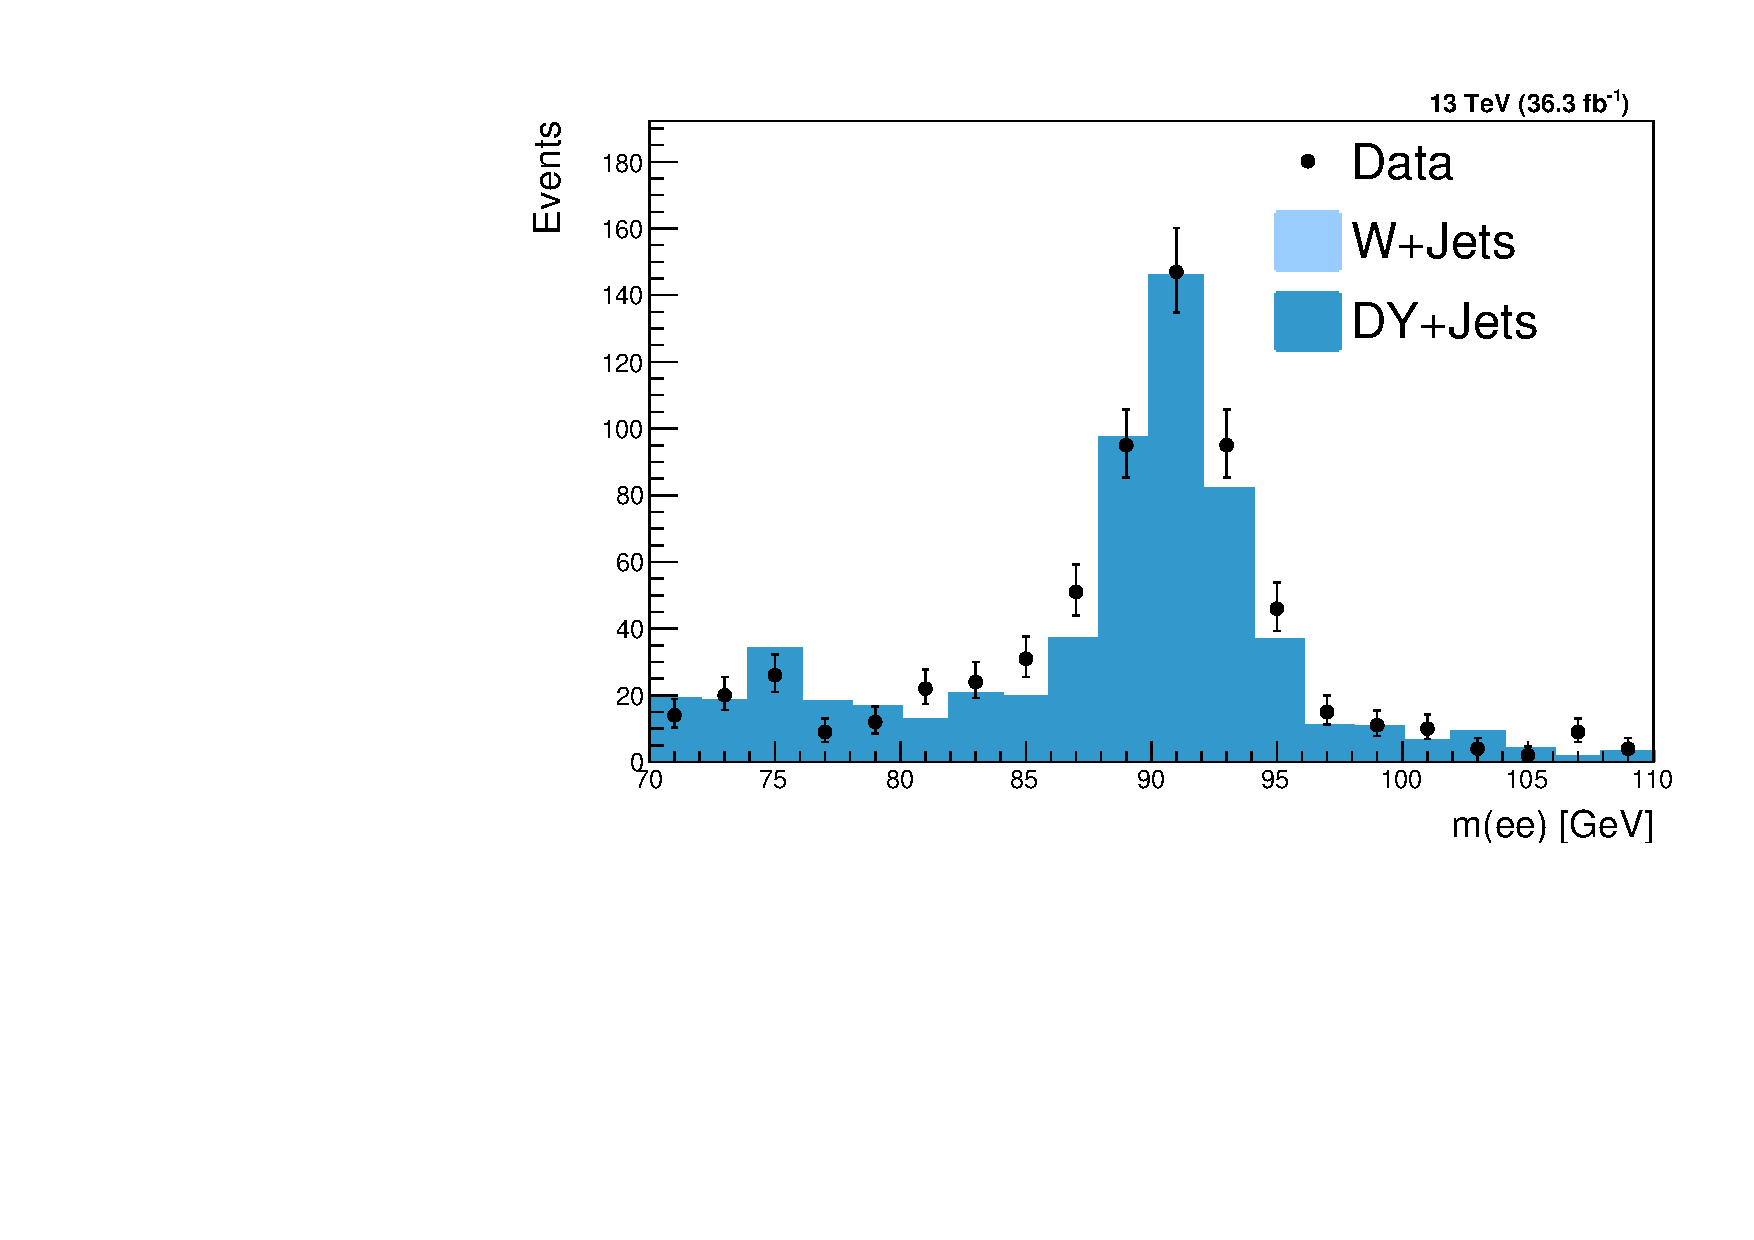
\includegraphics[width=\linewidth]{figs/05_analysis/2016_ZX_Z_mass_ELE_preselection_med.pdf} \\
	\end{tabular}
	\caption[m$\left(\ell^+\ell^-\right)$ data and simulated background after preselection criteria across all years in the anti-ID control region.]{m$\left(\ell^+\ell^-\right)$ data and simulated background after preselection criteria across all years in the anti-ID control region. Top row: $\PZ\to\PGm\PGm$ category. Bottom row: $\PZ\to\Pe\Pe$ category}
	\label{fig:zmass_preselection_med}
\end{figure}
\begin{figure}[htb!]
	\begin{tabular}{>{\centering\arraybackslash}m{0.32\linewidth} >{\centering\arraybackslash}m{0.32\linewidth} >{\centering\arraybackslash}m{0.32\linewidth}}
		2018 $\PZ\to\PGm\PGm$ & 2017 $\PZ\to\PGm\PGm$ & 2016 $\PZ\to\PGm\PGm$\\		
		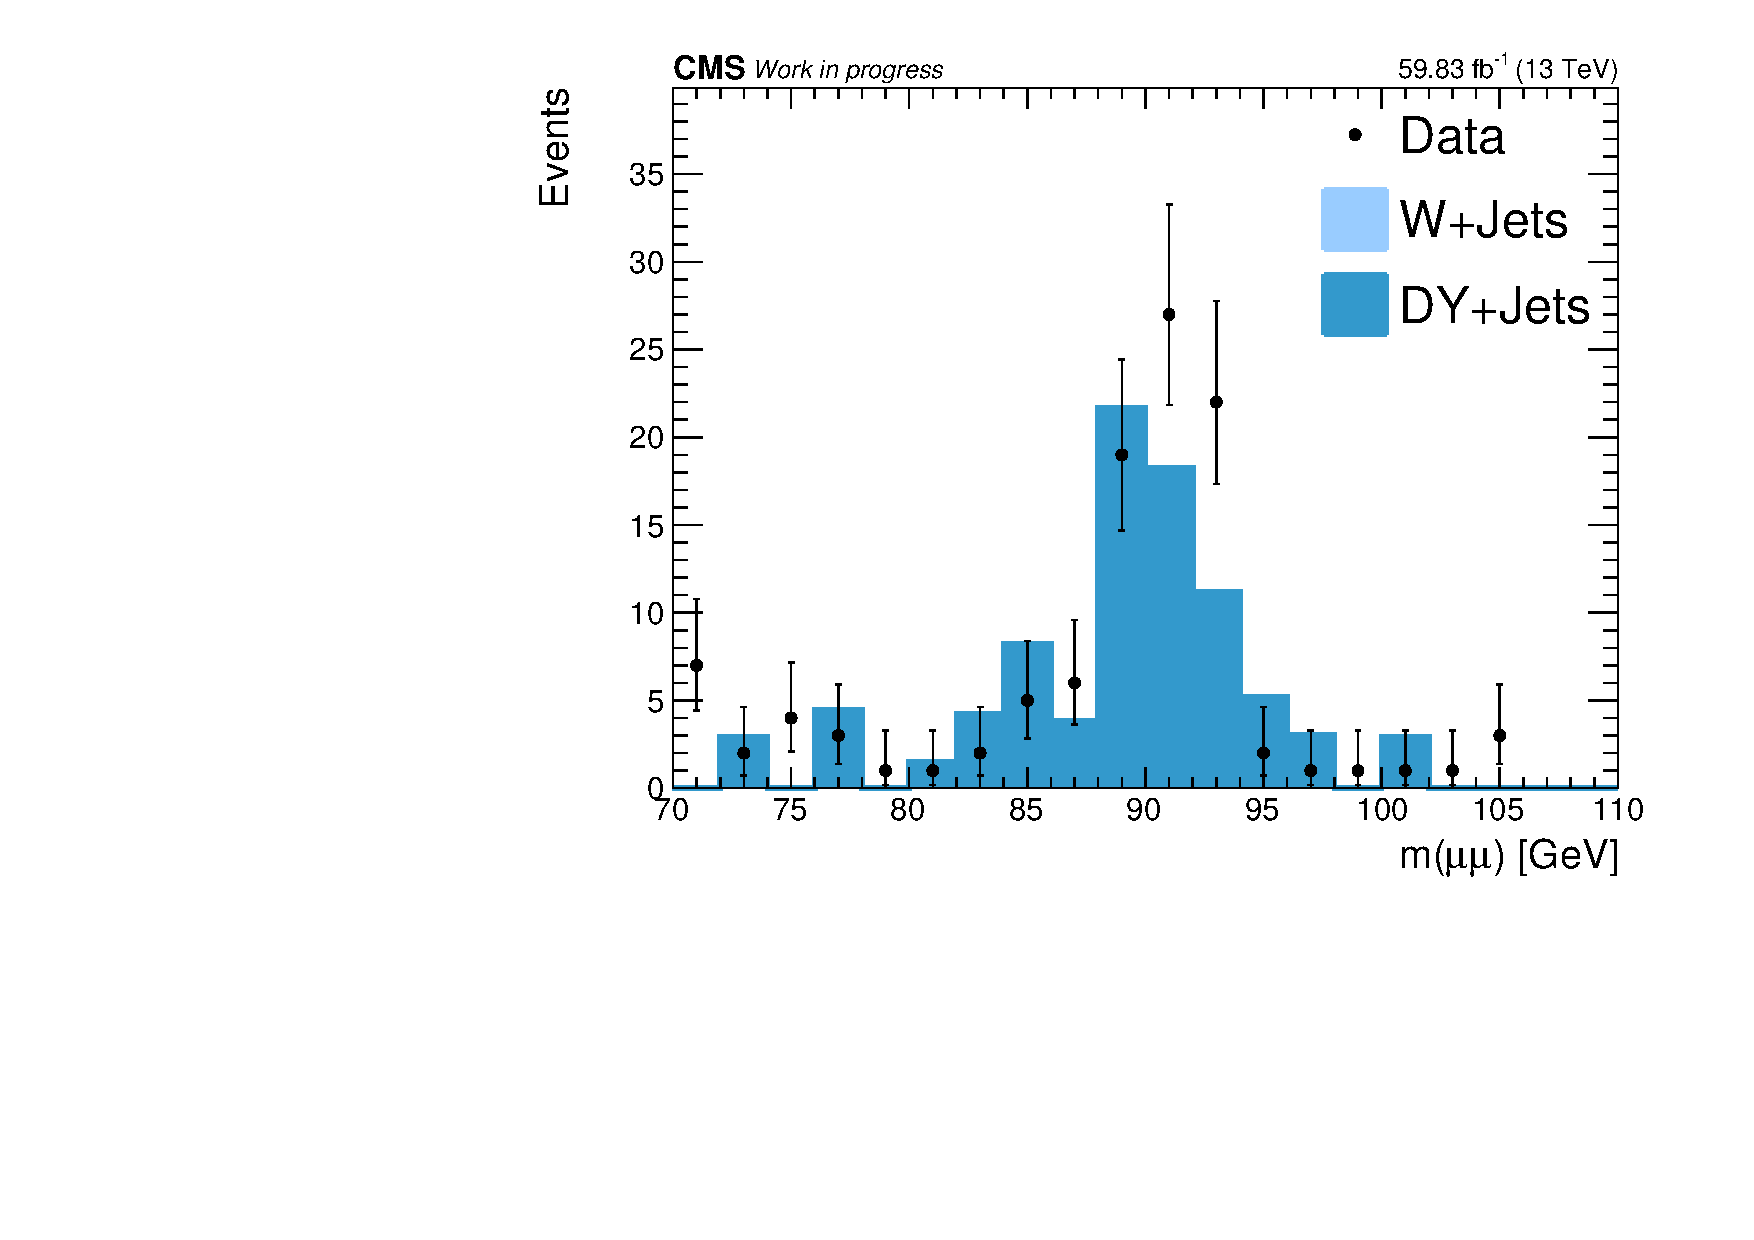
\includegraphics[width=\linewidth]{figs/05_analysis/2018_ZX_Z_mass_MU_preselection_tight.pdf} &
		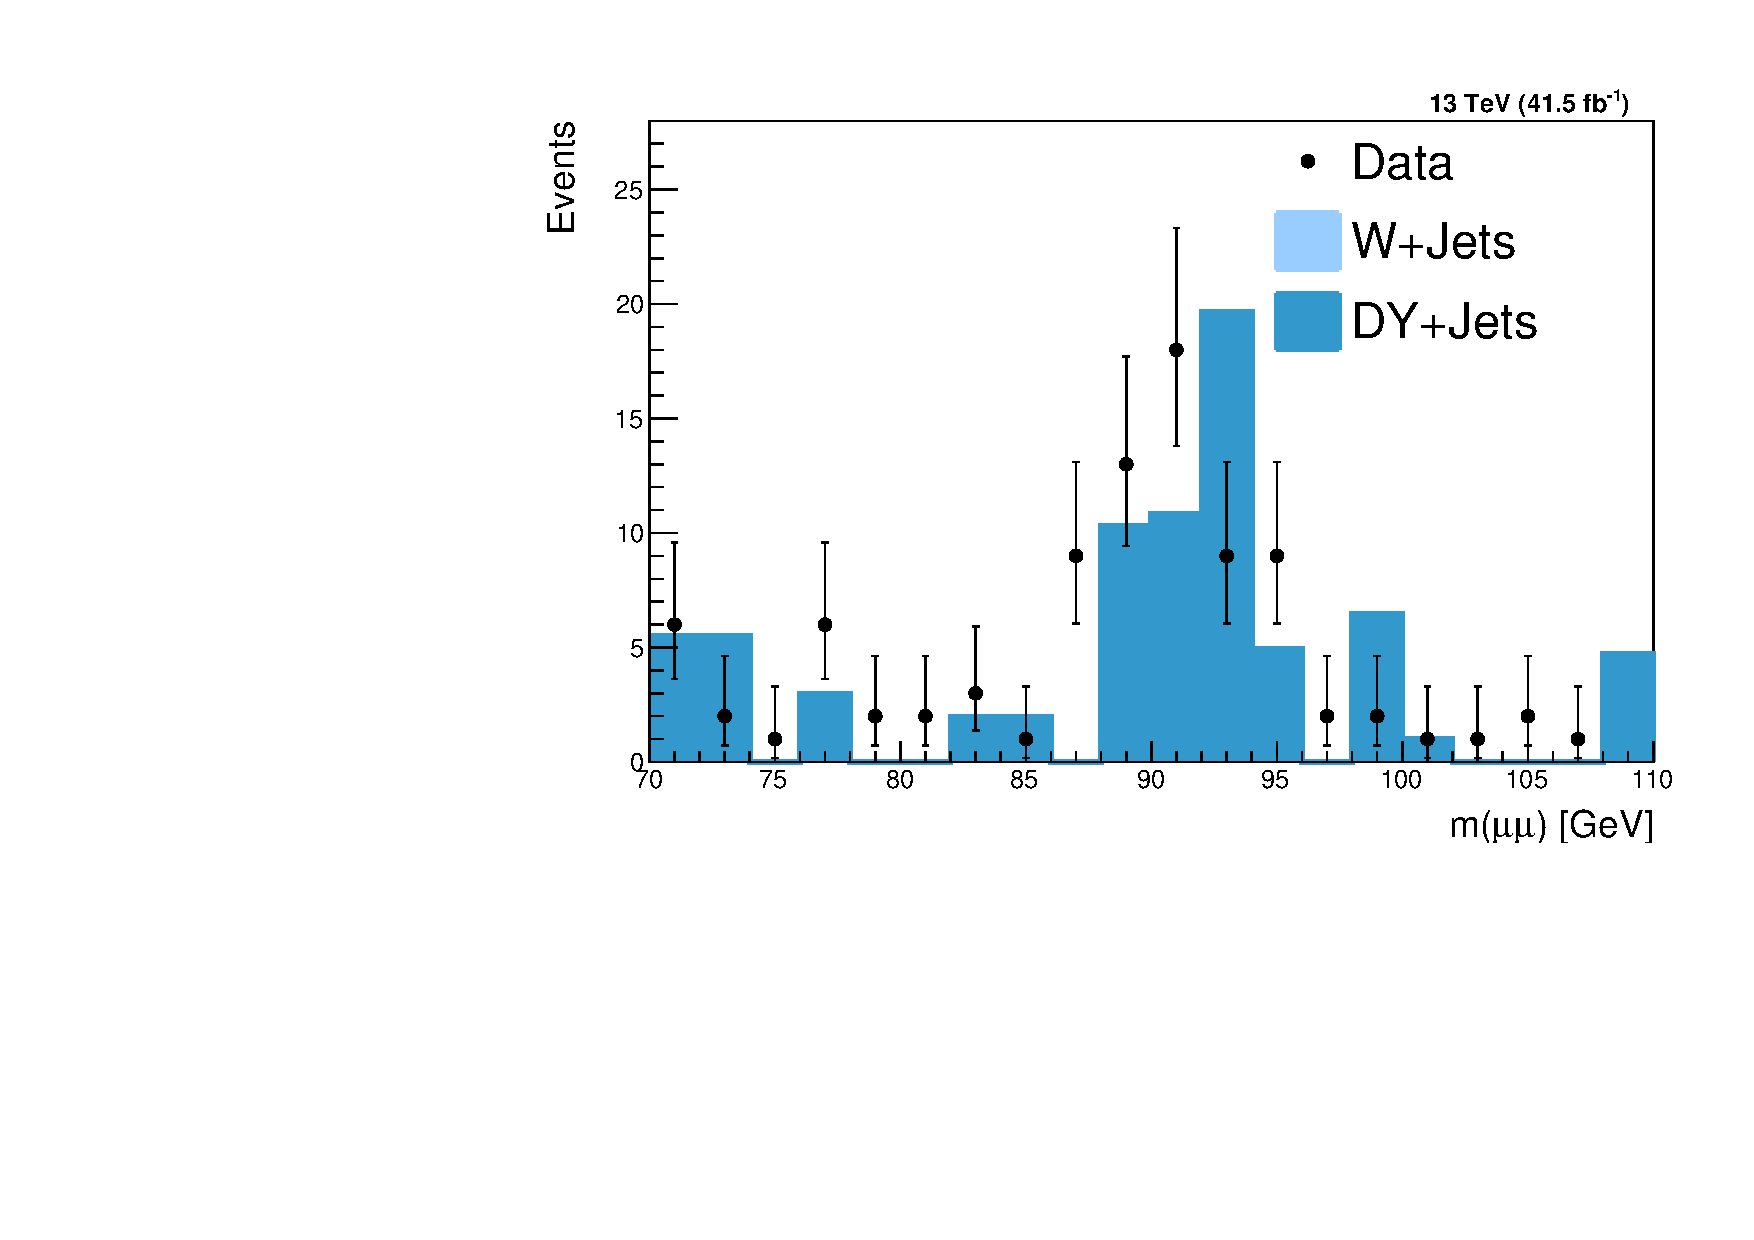
\includegraphics[width=\linewidth]{figs/05_analysis/2017_ZX_Z_mass_MU_preselection_tight.pdf} &
		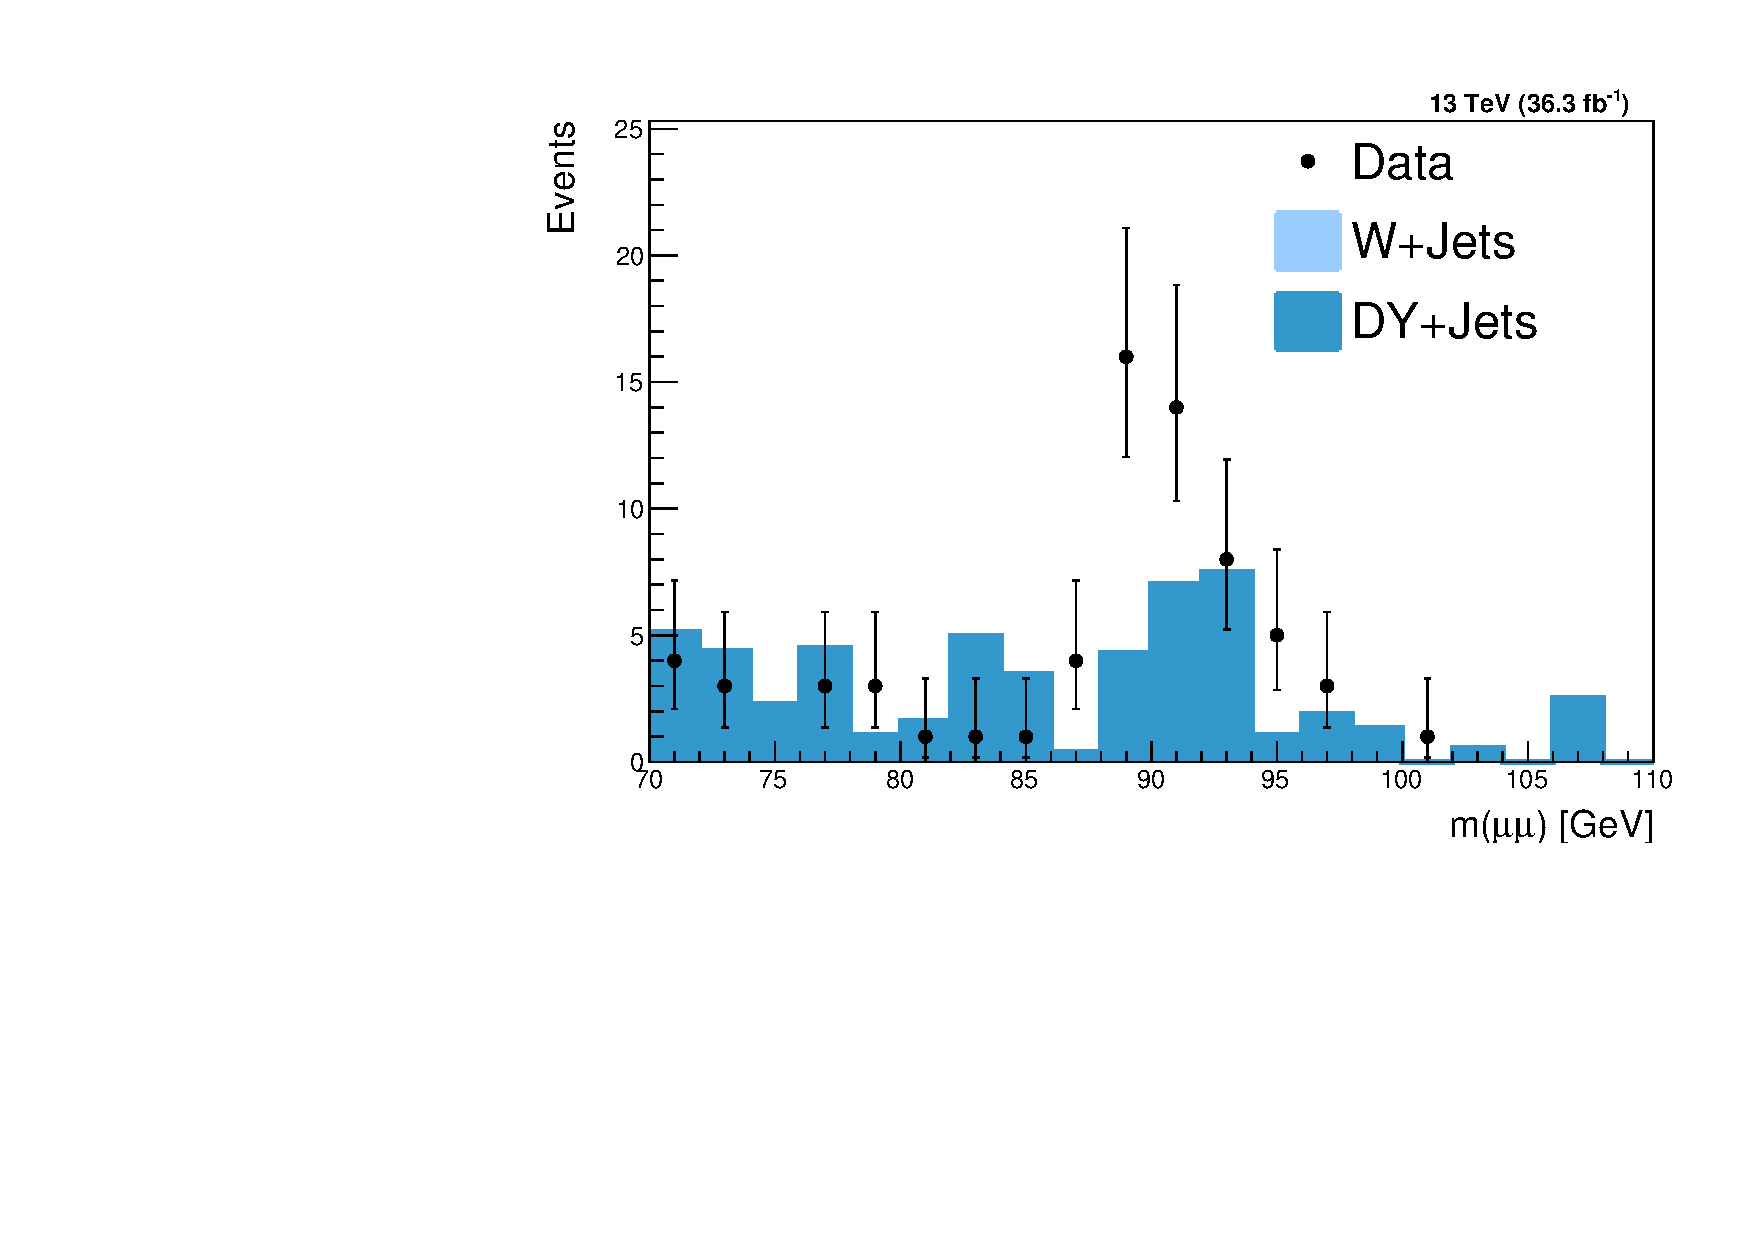
\includegraphics[width=\linewidth]{figs/05_analysis/2016_ZX_Z_mass_MU_preselection_tight.pdf} \\
		2018 $\PZ\to\Pe\Pe$ & 2017 $\PZ\to\Pe\Pe$ & 2016 $\PZ\to\Pe\Pe$\\		
		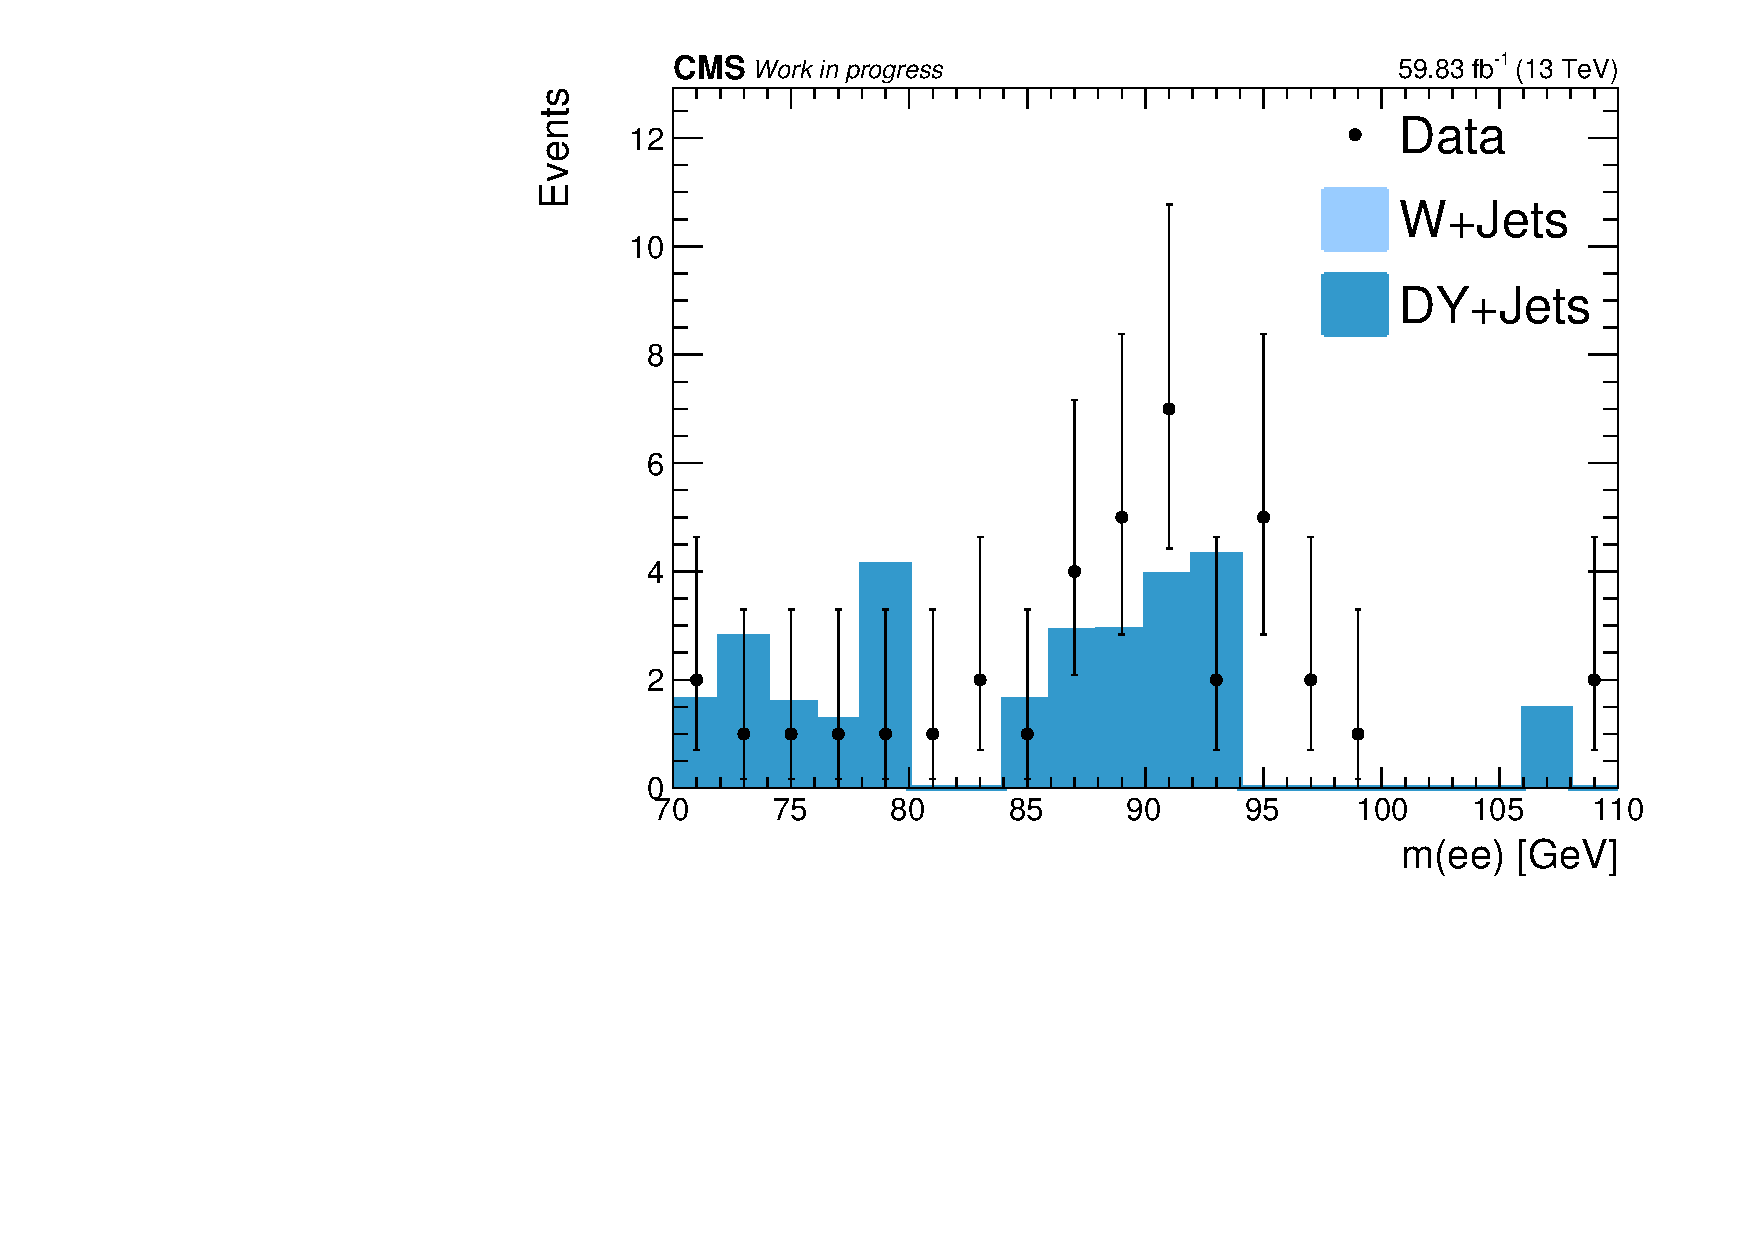
\includegraphics[width=\linewidth]{figs/05_analysis/2018_ZX_Z_mass_ELE_preselection_tight.pdf} &
		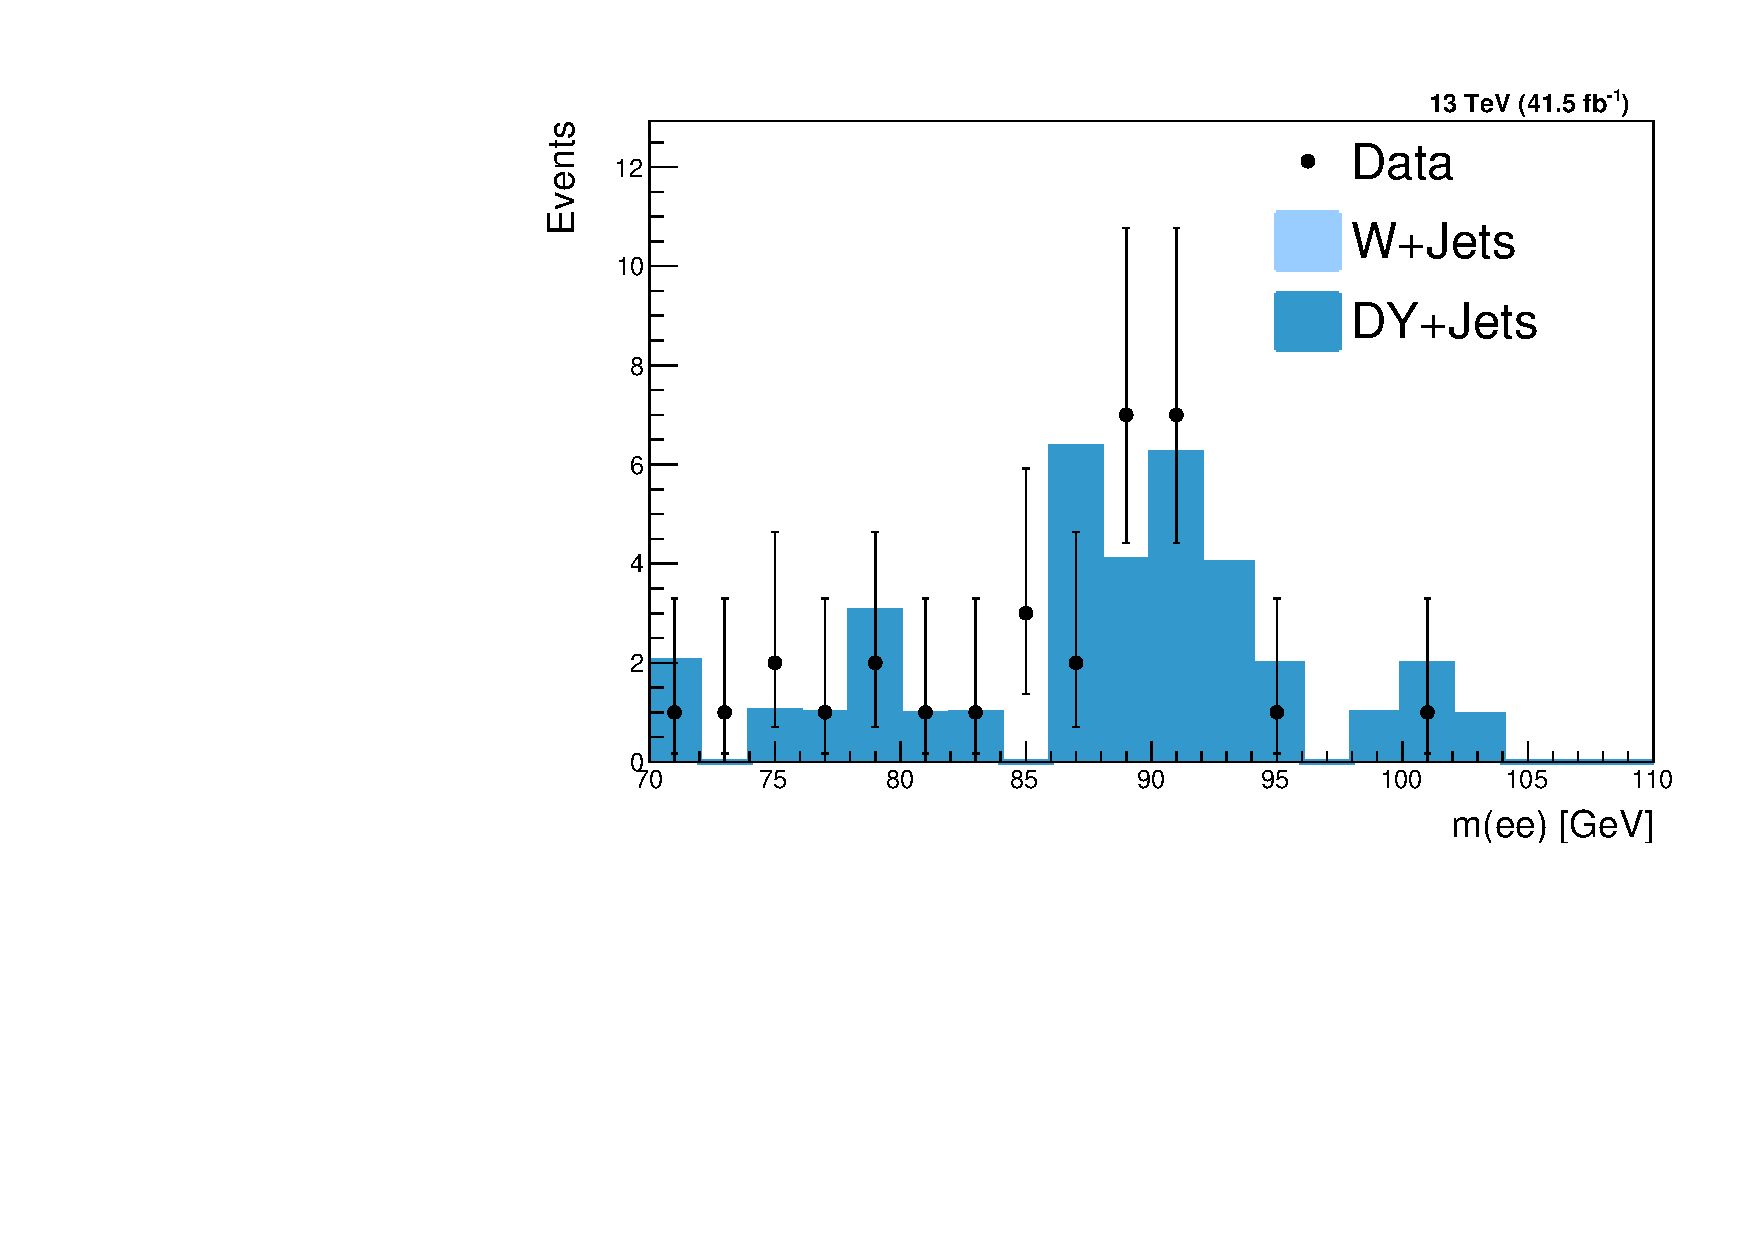
\includegraphics[width=\linewidth]{figs/05_analysis/2017_ZX_Z_mass_ELE_preselection_tight.pdf} &
		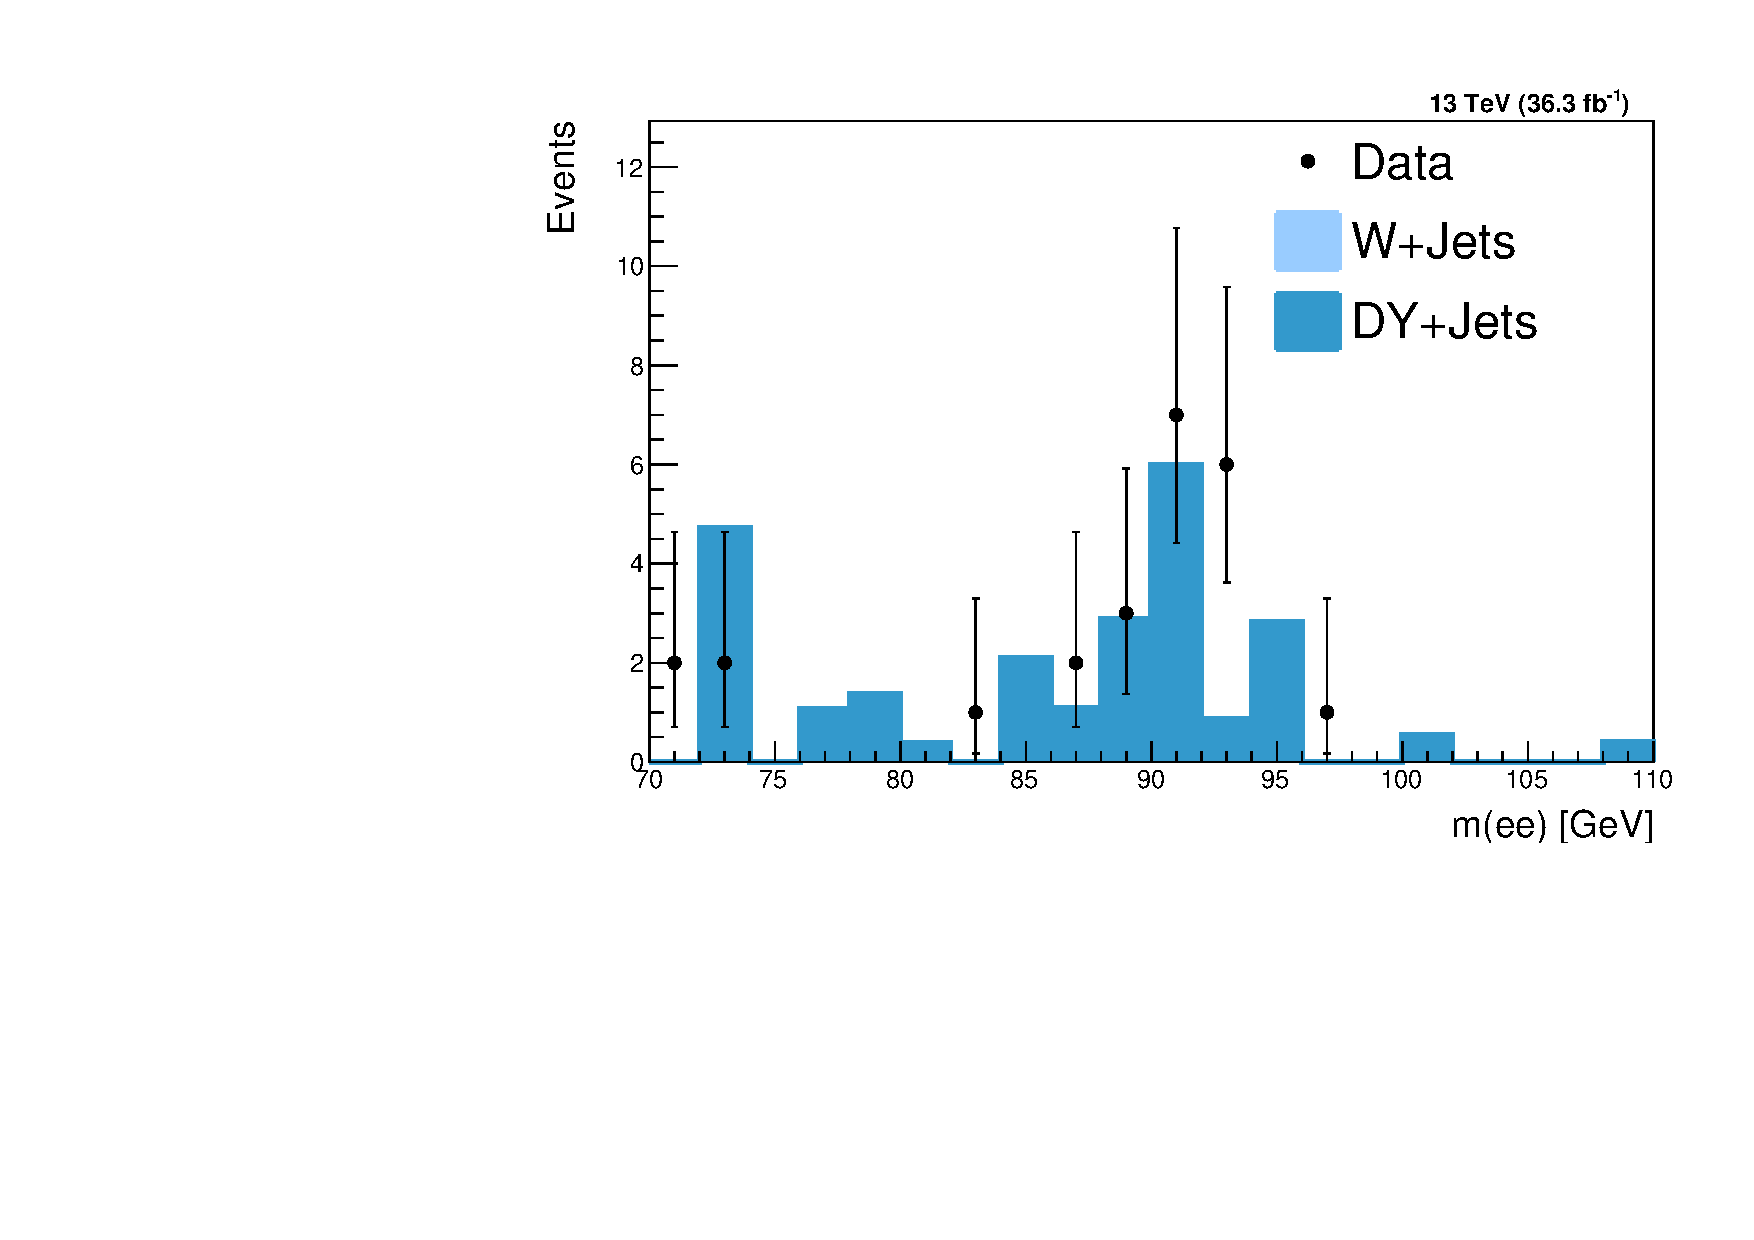
\includegraphics[width=\linewidth]{figs/05_analysis/2016_ZX_Z_mass_ELE_preselection_tight.pdf} \\
	\end{tabular}
	\caption[m$\left(\ell^+\ell^-\right)$ data and simulated background after preselection criteria across all years in the ID signal region.]{m$\left(\ell^+\ell^-\right)$ data and simulated background after preselection criteria across all years in the ID signal region. Top row: $\PZ\to\PGm\PGm$ category. Bottom row: $\PZ\to\Pe\Pe$ category}
	\label{fig:zmass_preselection_tight}
\end{figure}

\subsubsection{Positive and Negative \lxy Regions} \label{sec:ana_lxyregions}
As discussed in section~\ref{sec:ana_vertex}, it is possible for the vertex calculating to yield a negative value of \lxy, indicating that the $\Phi$ would have decayed from behind the beamline relative to the ECAL clusters. The negative \lxy region is used for background estimation, while the positive \lxy region is used for the final signal extraction. To avoid possible signal contamination in the negative \lxy region, we define the two regions using the prompt invariant diphoton mass \mgg. This provides a robust cut that is not dependent on the vertex calculation.

By construction of the vertex constraint, if two photons have a prompt invariant mass $\mgg$ then the vertex calculated assuming $\mphi=\mgg$ would yield an $\lxy=0$. As a corollary, the prompt invariant mass of a pair of displaced photons decaying from a particle of mass $\mphi$ will always have a prompt invariant mass $\mgg\leq\mphi$. Since the mass of the $\Phi$ is constrained by a maximum of $\mh/2$, the highest prompt invariant mass for potential signal events is $\mgg=\mh/2$. Thus cutting on $\mgg>\mh/2$ gives a set of events that yield a negative \lxy for all hypothetical \mphi that is disjoint from any possible signal events.

The positive \lxy signal region is defined by $\mgg<\mphi+5\GeV$. This allows slightly negative \lxy events into the signal region in order to account for the vertex calculation resolution for low displacement signal events.

\subsubsection{Final State Radiation Rejection} \label{sec:ana_fsr}
One source of background occurs when a lepton in the final state radiates a photon, known as final state radiation (FSR). This results in the band of excess events in \mll seen in figures~\ref{fig:zmass_preselection_med}$\,$-$\,$\ref{fig:zmass_preselection_tight}. FSR events are identified by calculating the invariant mass of the dileptons plus one or both of the photons used to reconstruct the $\Phi$ candidate. If the combined invariant mass is within $75-105\GeV$ and closer to the \PZ boson mass of 91\GeV than the original dilepton mass, the event is flagged as having FSR and removed. FSR events are classified based on which combination of photons yields a mass within the \PZ window, with the closest mass to 91\GeV being chosen if multiple satisfy the criteria. The categories are defined as follows:
\begin{itemize}
	\item Tag 1: $\ell\ell+\gamma_1$
	\item Tag 2: $\ell\ell+\gamma_2$
	\item Tag 3: $\ell\ell+\gamma_1+\gamma_2$
\end{itemize}

Figure~\ref{fig:fsr_distributions} show the comparison of invariant mass distributions for all three tags in the $\PZ\to\PGm\PGm$ category. Simulated background uses the anti-ID control region due to poor statistical power in the ID signal region. Simulated signal uses an $\mphi=20\GeV$, $c\tau=0\unit{mm}$ signal sample, but the distributions remain stable across all masses and lifetimes. It is shown that the largest background contribution comes from tag 2 followed by tag 1. Tag 3 shows minimal contribution, as the energy loss from double FSR photons usually causes the dilepton invariant mass to fall below 70\GeV. 

\begin{figure}[htb!]
	\centering
	\captionsetup[subfigure]{justification=centering}
	\begin{subfigure}[h]{.32\linewidth}
		\centering
		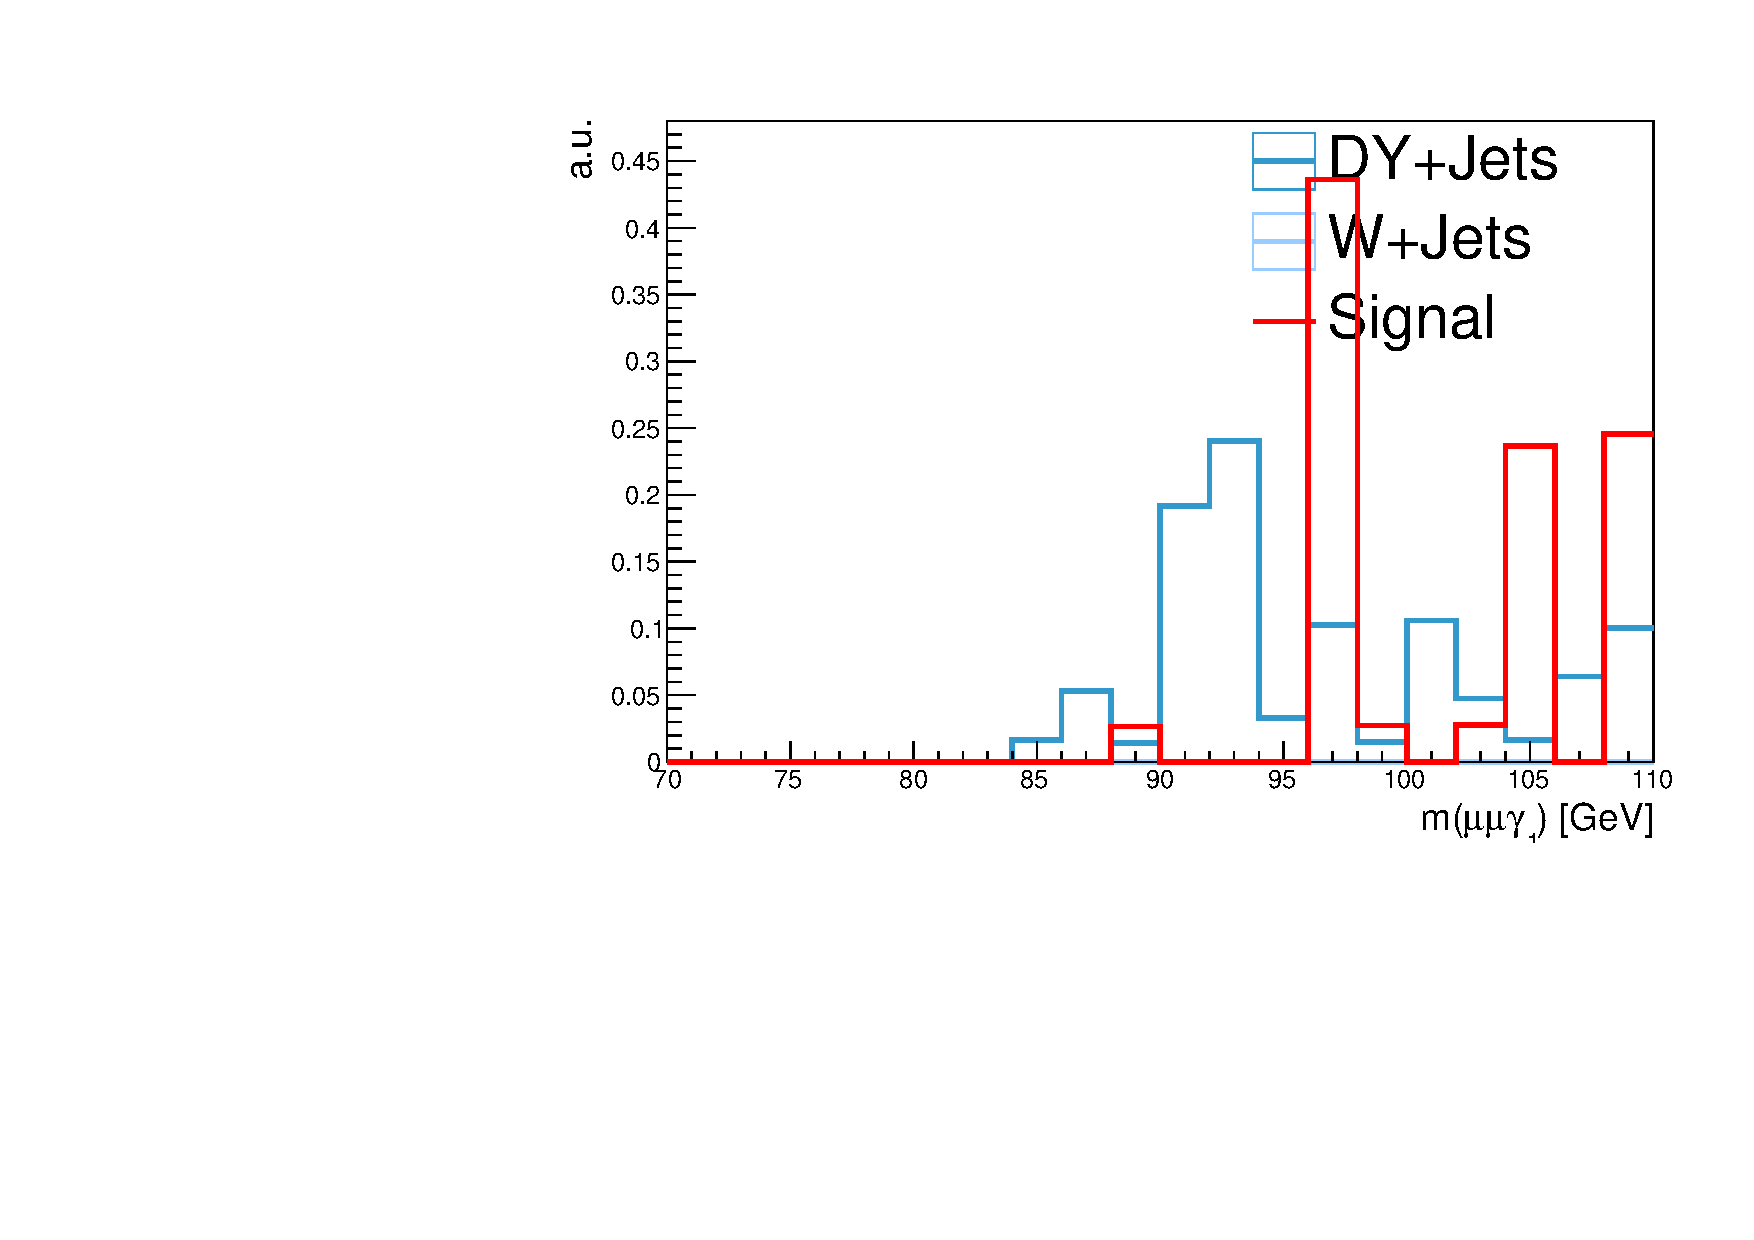
\includegraphics[width=\linewidth]{figs/05_analysis/2018_ZX_Zg1_mass_MU_preFSR_mx20_comp.pdf}
		\caption{m($\PGm\PGm\gamma_1$)}
	\end{subfigure}
	\begin{subfigure}[h]{.32\linewidth}
		\centering
		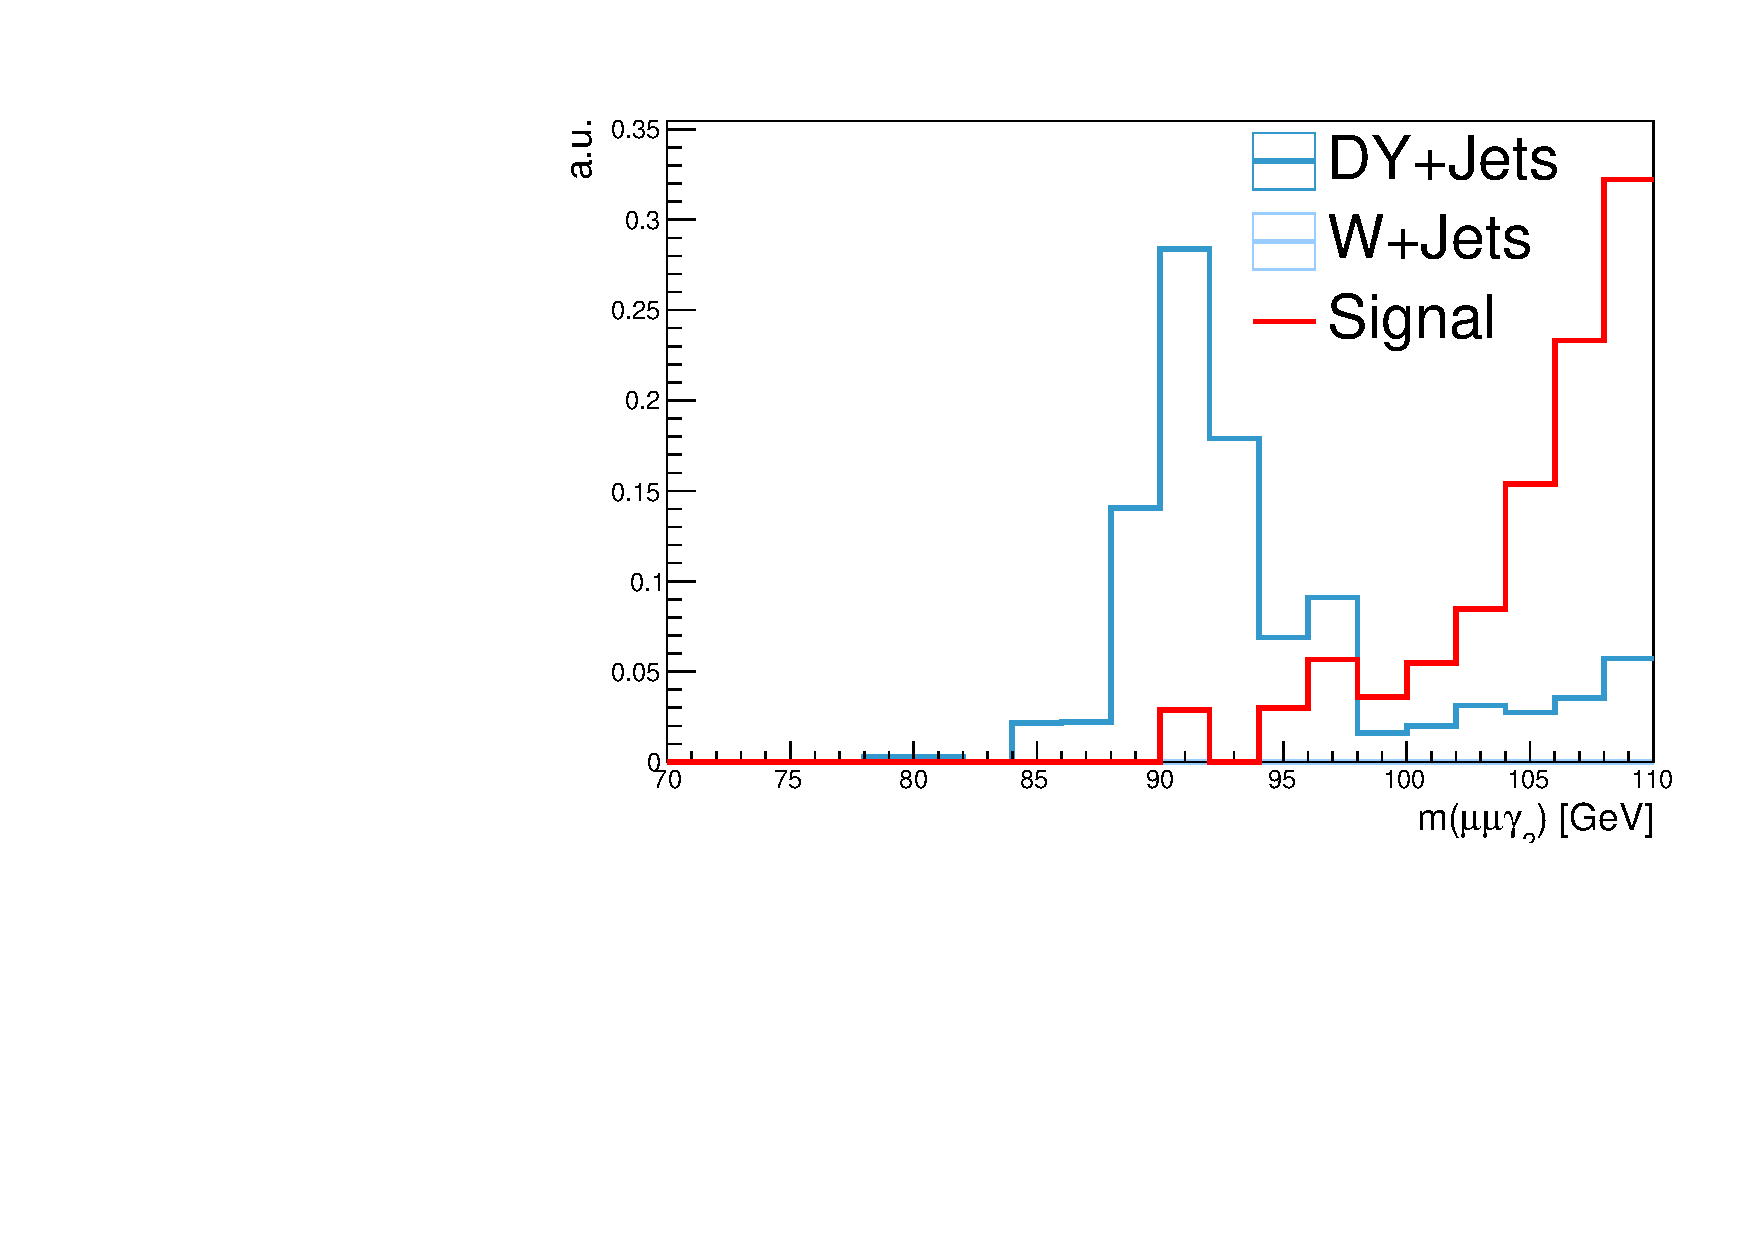
\includegraphics[width=\linewidth]{figs/05_analysis/2018_ZX_Zg2_mass_MU_preFSR_mx20_comp.pdf}
		\caption{m($\PGm\PGm\gamma_2$)}
	\end{subfigure}
	\begin{subfigure}[h]{.32\linewidth}
		\centering
		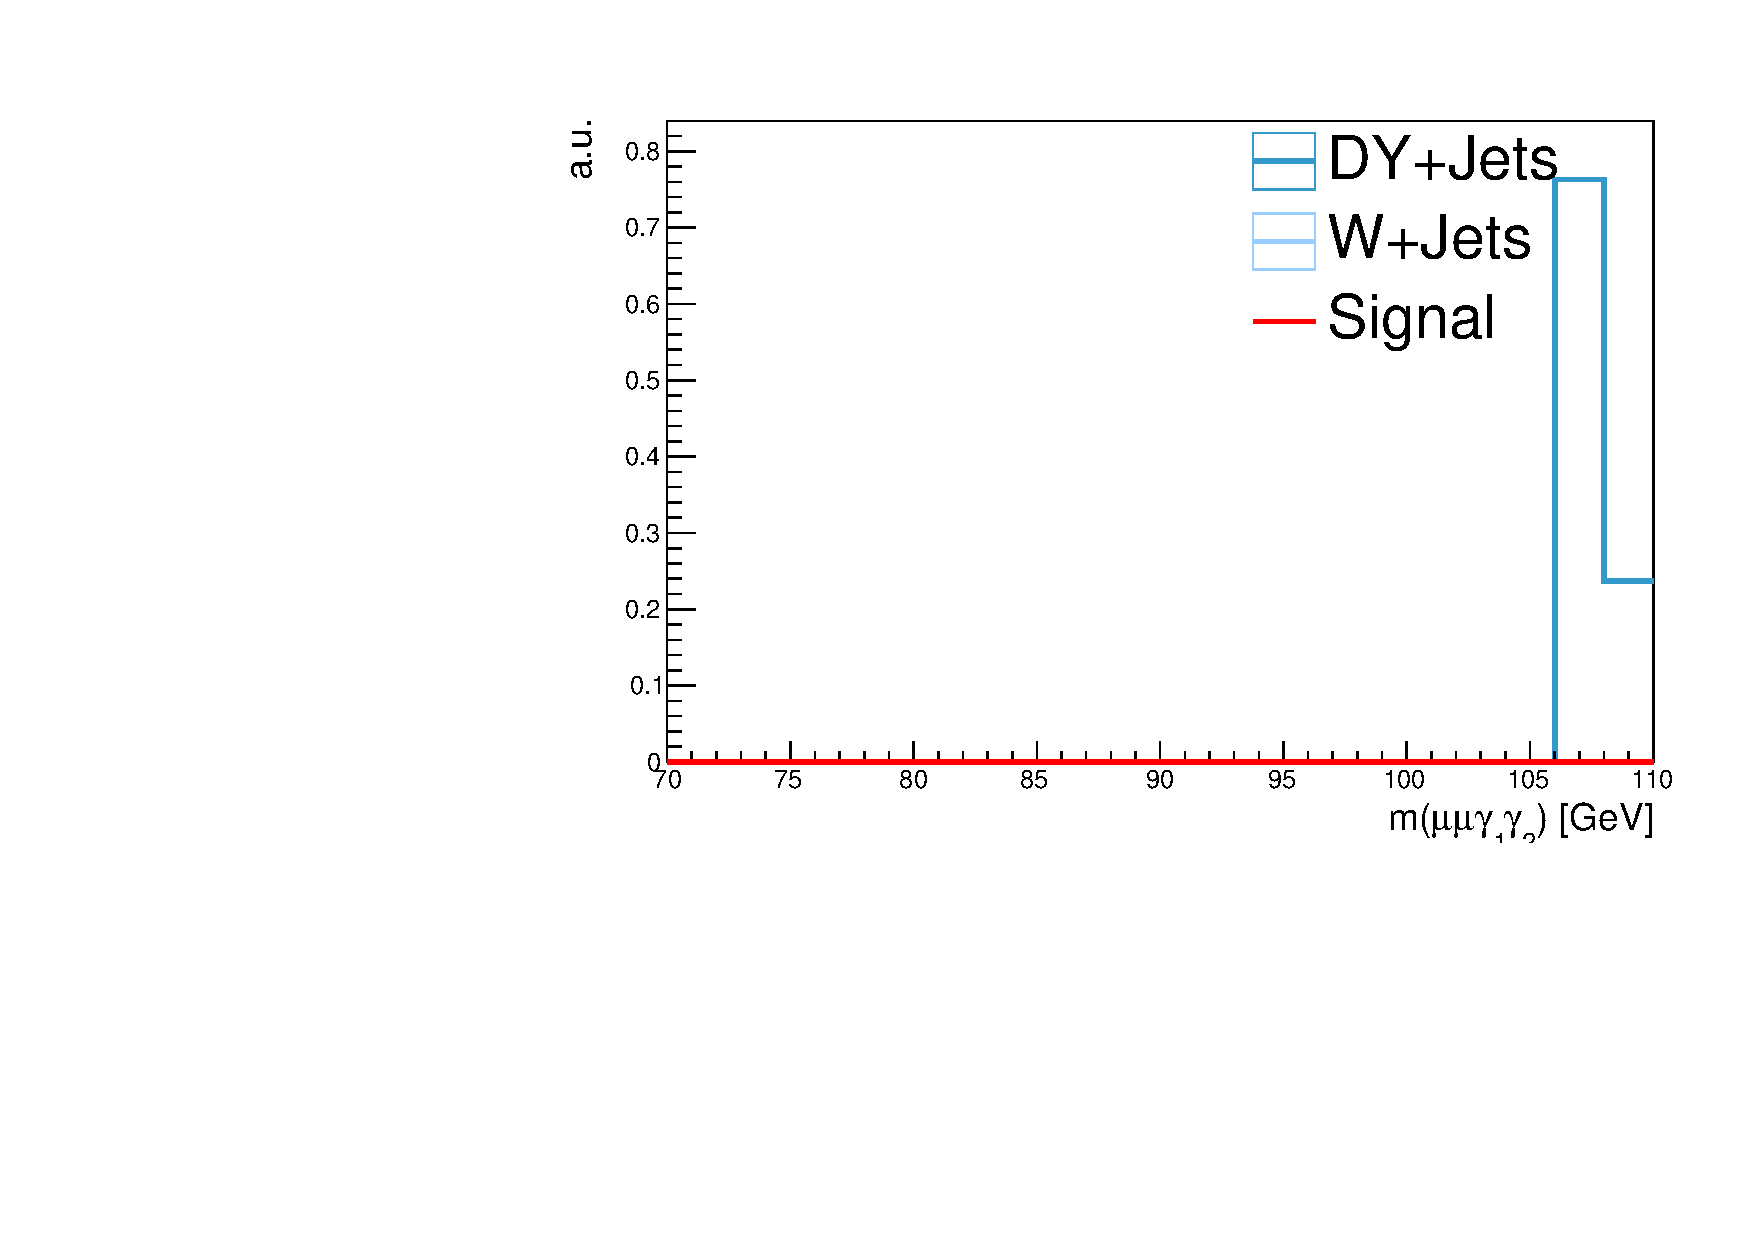
\includegraphics[width=\linewidth]{figs/05_analysis/2018_ZX_mass_MU_preFSR_mx20_comp.pdf}
		\caption{m($\PGm\PGm\gamma_1\gamma_2$)}
	\end{subfigure}
	\begin{subfigure}[h]{.32\linewidth}
		\centering
		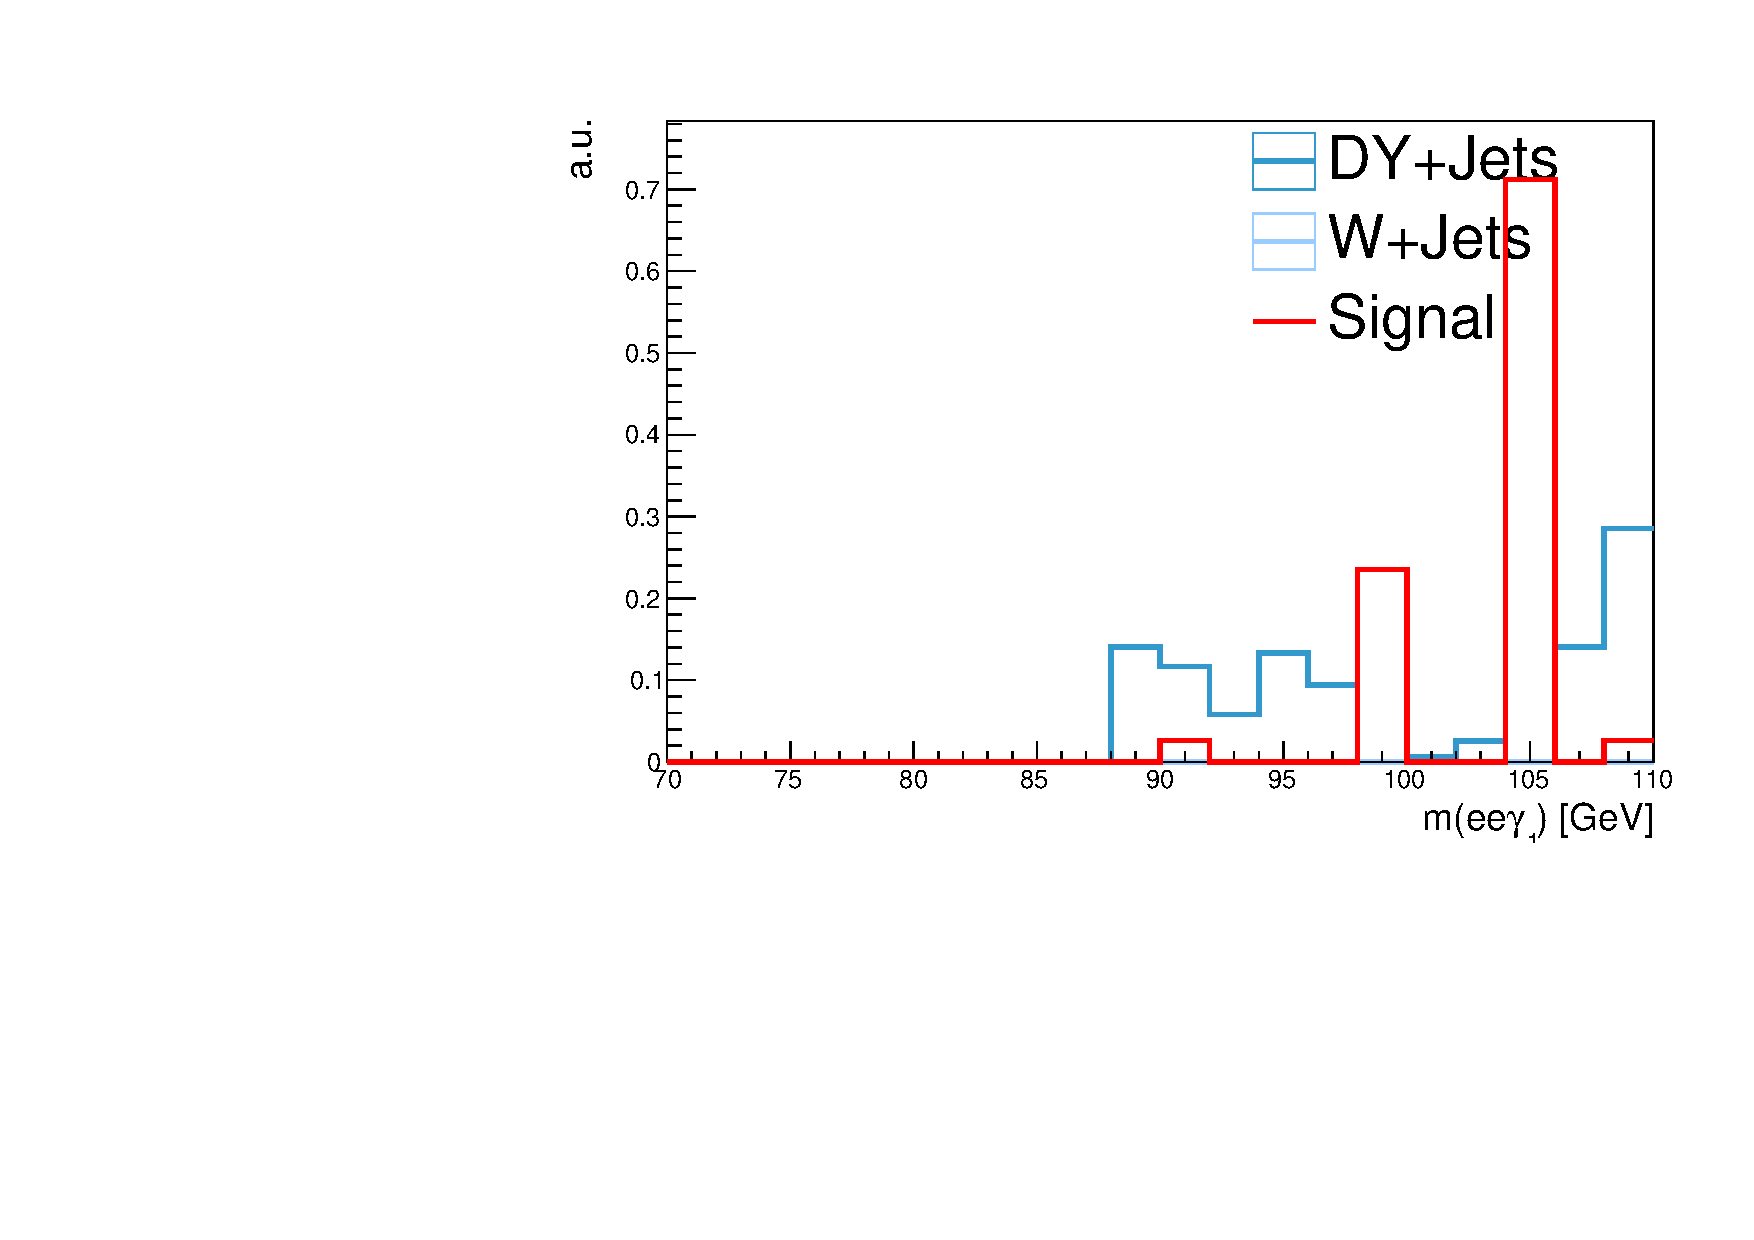
\includegraphics[width=\linewidth]{figs/05_analysis/2018_ZX_Zg1_mass_ELE_preFSR_mx20_comp.pdf}
		\caption{m($ee\gamma_1$)}
	\end{subfigure}
	\begin{subfigure}[h]{.32\linewidth}
		\centering
		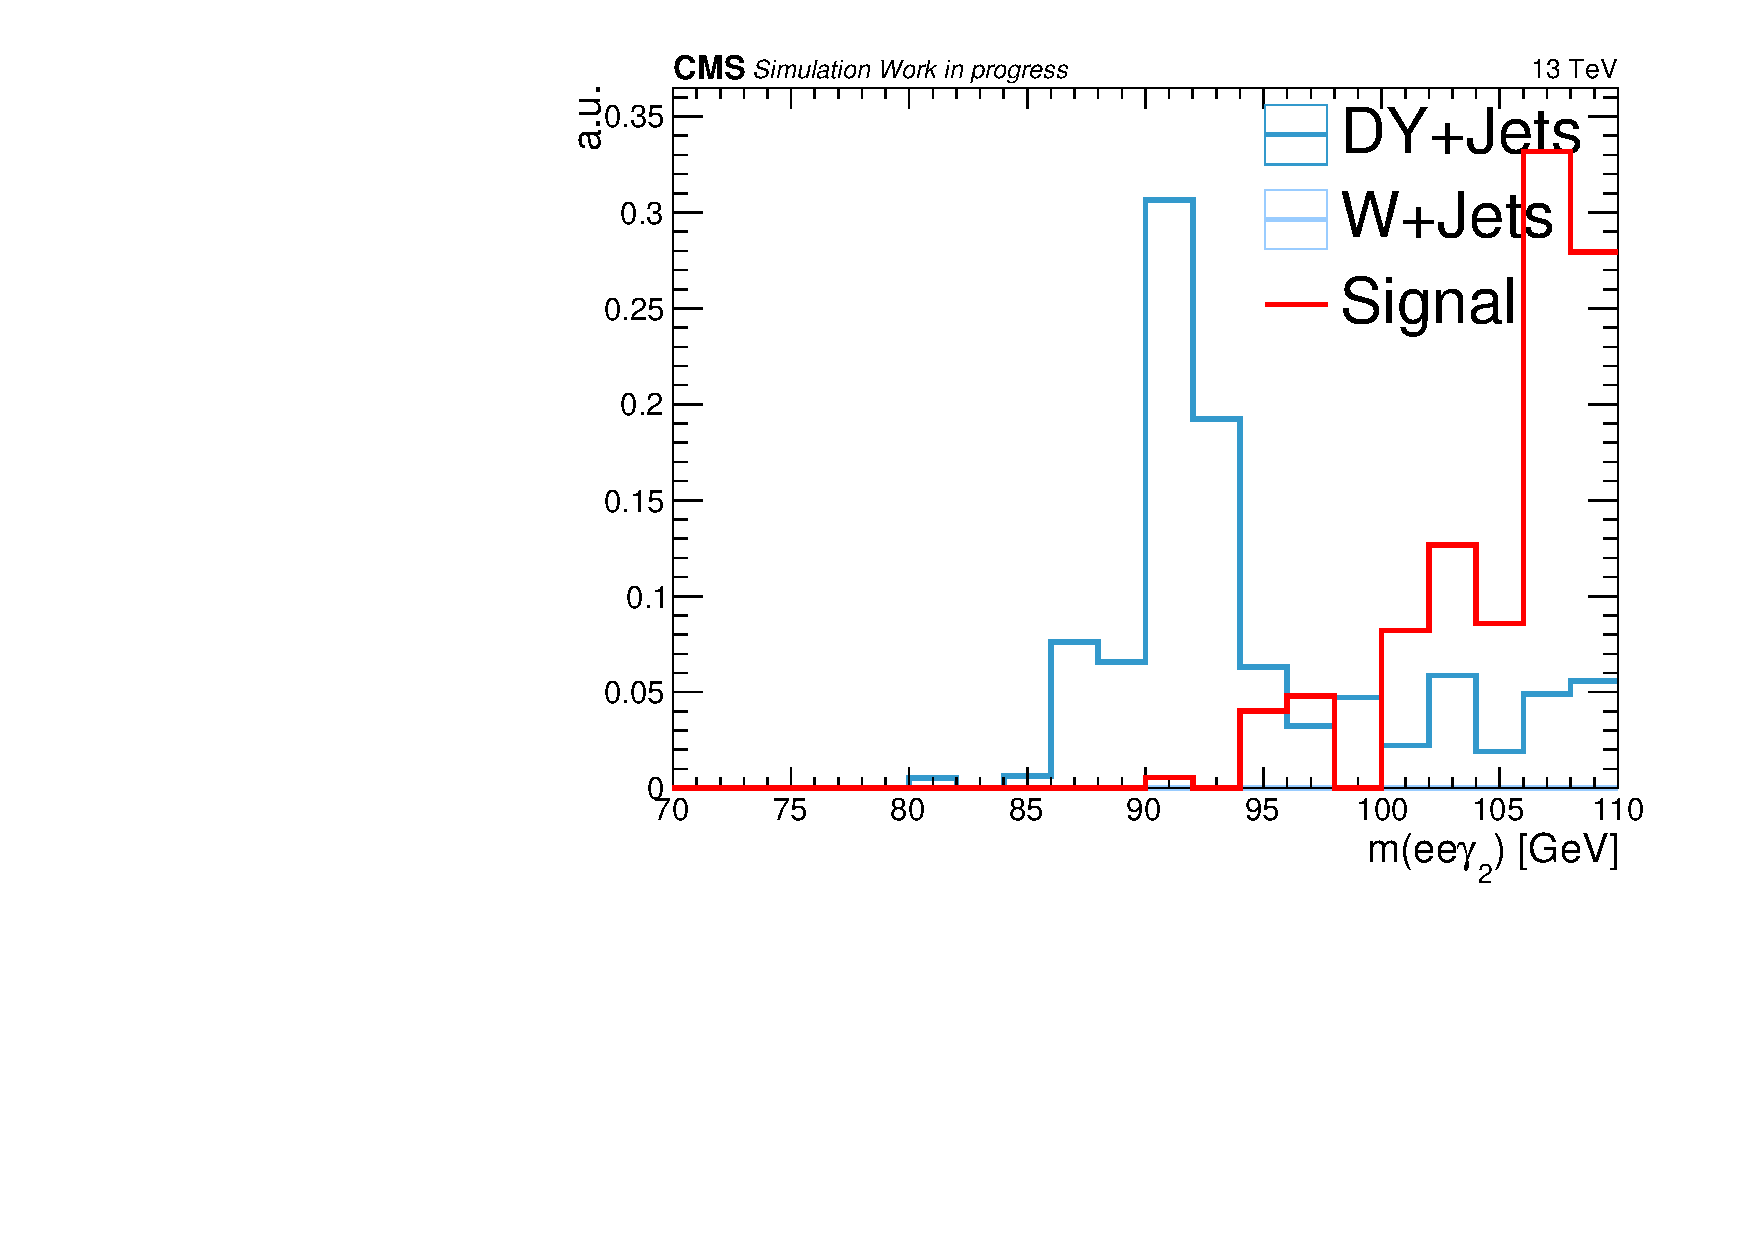
\includegraphics[width=\linewidth]{figs/05_analysis/2018_ZX_Zg2_mass_ELE_preFSR_mx20_comp.pdf}
		\caption{m($ee\gamma_2$)}
	\end{subfigure}
	\begin{subfigure}[h]{.32\linewidth}
		\centering
		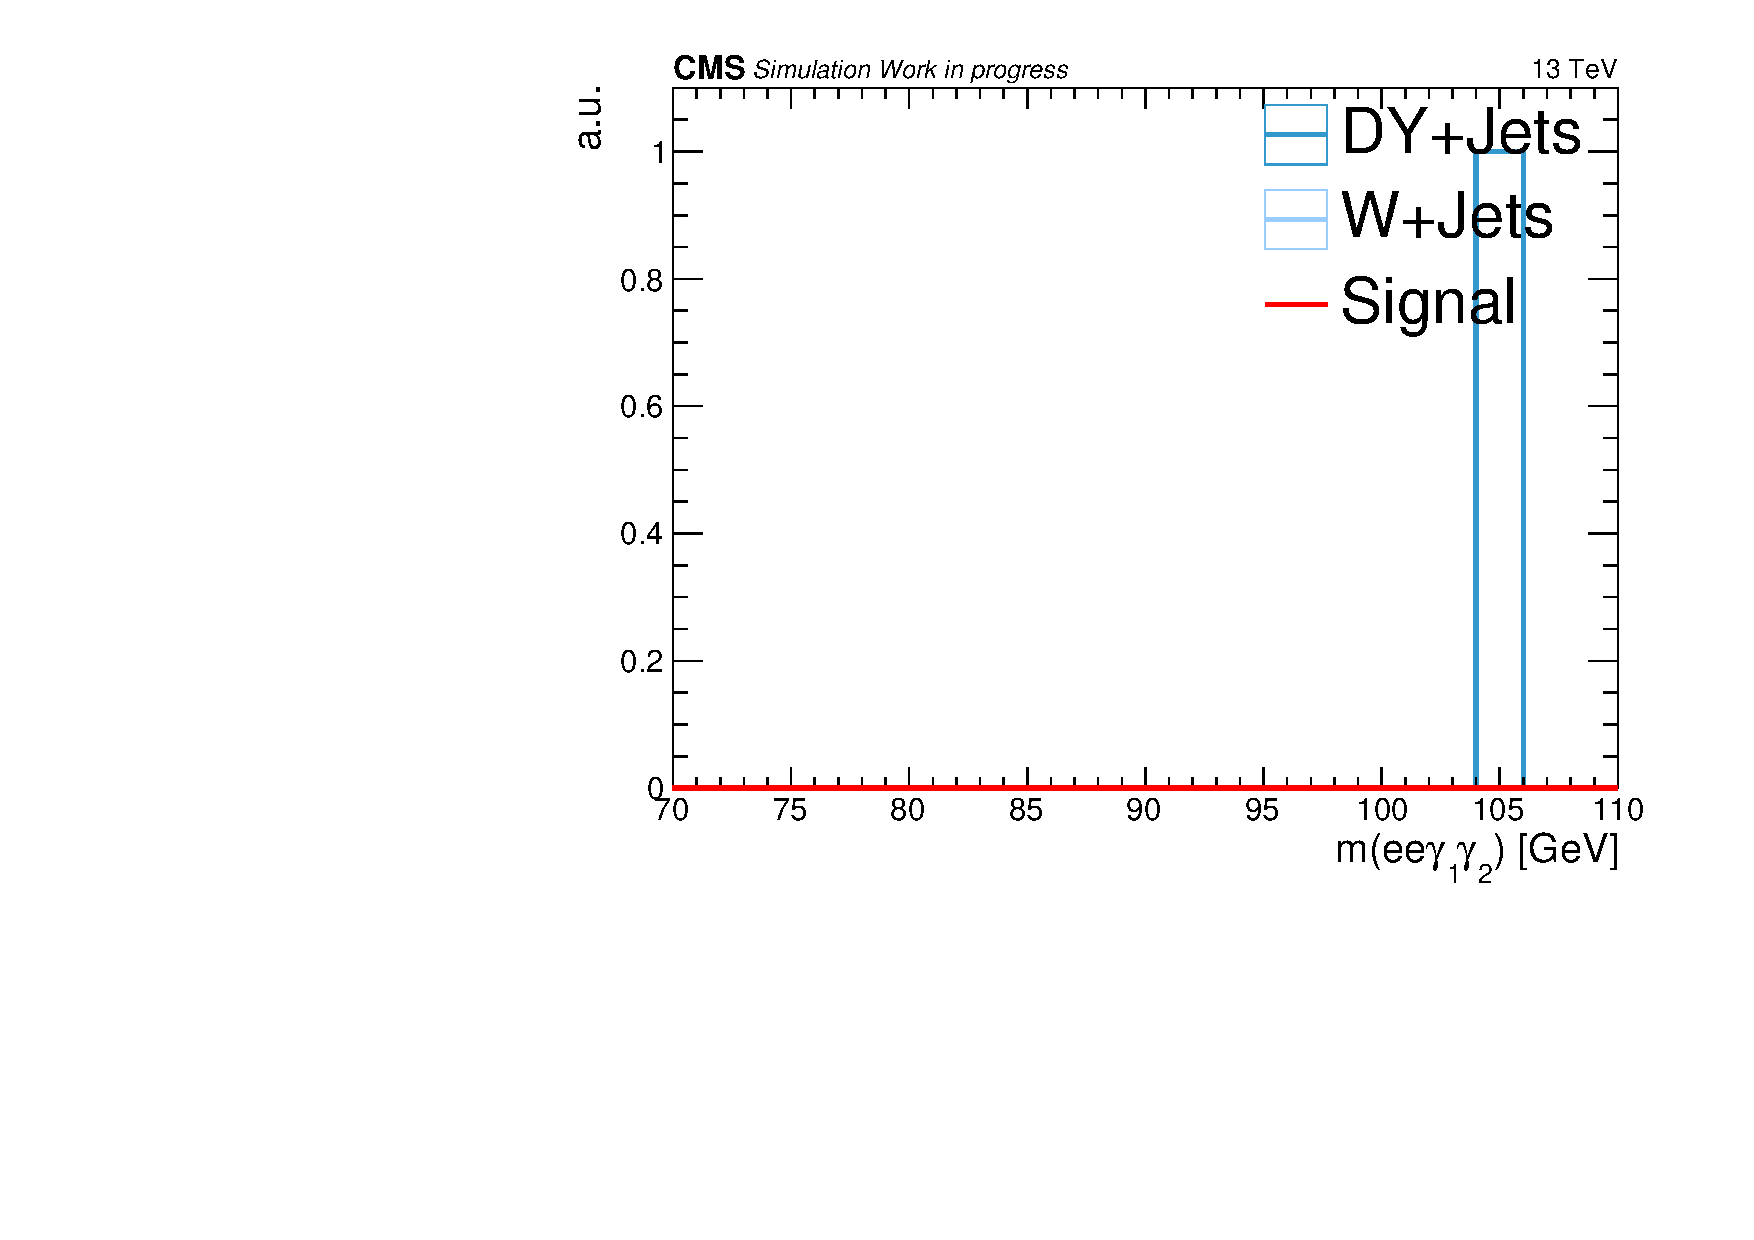
\includegraphics[width=\linewidth]{figs/05_analysis/2018_ZX_mass_ELE_preFSR_mx20_comp.pdf}
		\caption{m($ee\gamma_1\gamma_2$)}
	\end{subfigure}
	\caption[Comparison of invariant mass distributions for FSR rejection using simulated $\mphi=20\GeV$, $c\tau=0\unit{mm}$ signal and background. Background uses normalized anti-ID control region events for improved statistics while signal shows ID signal region events.]{Comparison of invariant mass distributions for FSR rejection using simulated $\mphi=20\GeV$, $c\tau=0\unit{mm}$ signal and background. Background uses normalized anti-ID control region events for improved statistics while signal shows ID signal region events.}
	\label{fig:fsr_distributions}
\end{figure}

In the anti-ID control region, this method rejects 16\% of simulated background in the $\PZ\to \PGm\PGm$ category and 19\% in the $\PZ\to\Pe\Pe$ category. In the ID signal region, this method rejects 9\% of simulated background in the $\PZ\to\PGm\PGm$ category and 35\% in the $\PZ\to\Pe\Pe$ category. Across all signal masses and lifetimes this method maintains $>99.5\%$ signal efficiency. The data and simulated background distributions after rejecting FSR events are shown in figures~\ref{fig:zmass_postFSR_med}$\,$-$\,$\ref{fig:zmass_postFSR_tight}.

\begin{figure}[htb!]
	\centering
	\begin{tabular}{>{\centering\arraybackslash}m{0.32\linewidth} >{\centering\arraybackslash}m{0.32\linewidth} >{\centering\arraybackslash}m{0.32\linewidth}}
		2018 $\PZ\to\PGm\PGm$ & 2017 $\PZ\to\PGm\PGm$ & 2016 $\PZ\to\PGm\PGm$\\
		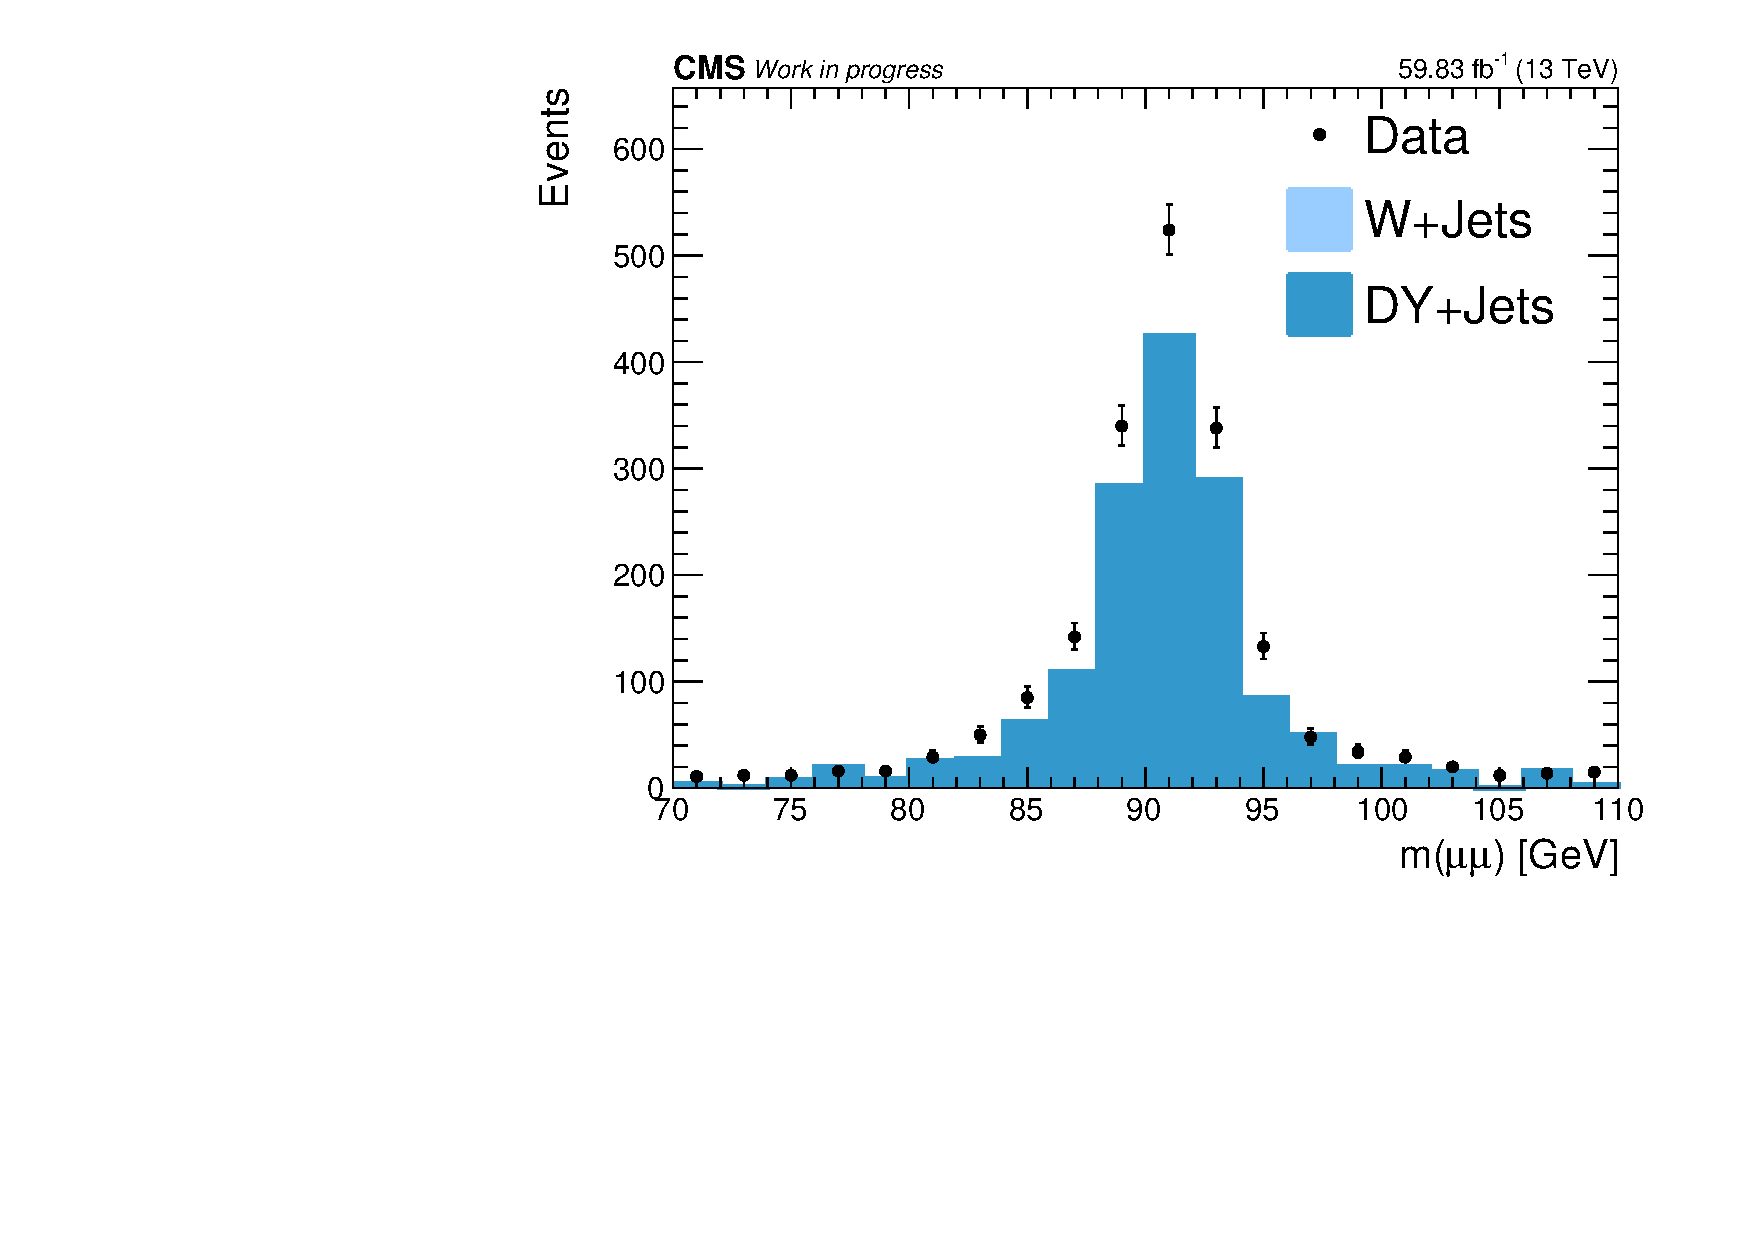
\includegraphics[width=\linewidth]{figs/05_analysis/2018_ZX_Z_mass_MU_postFSR_med.pdf} &
		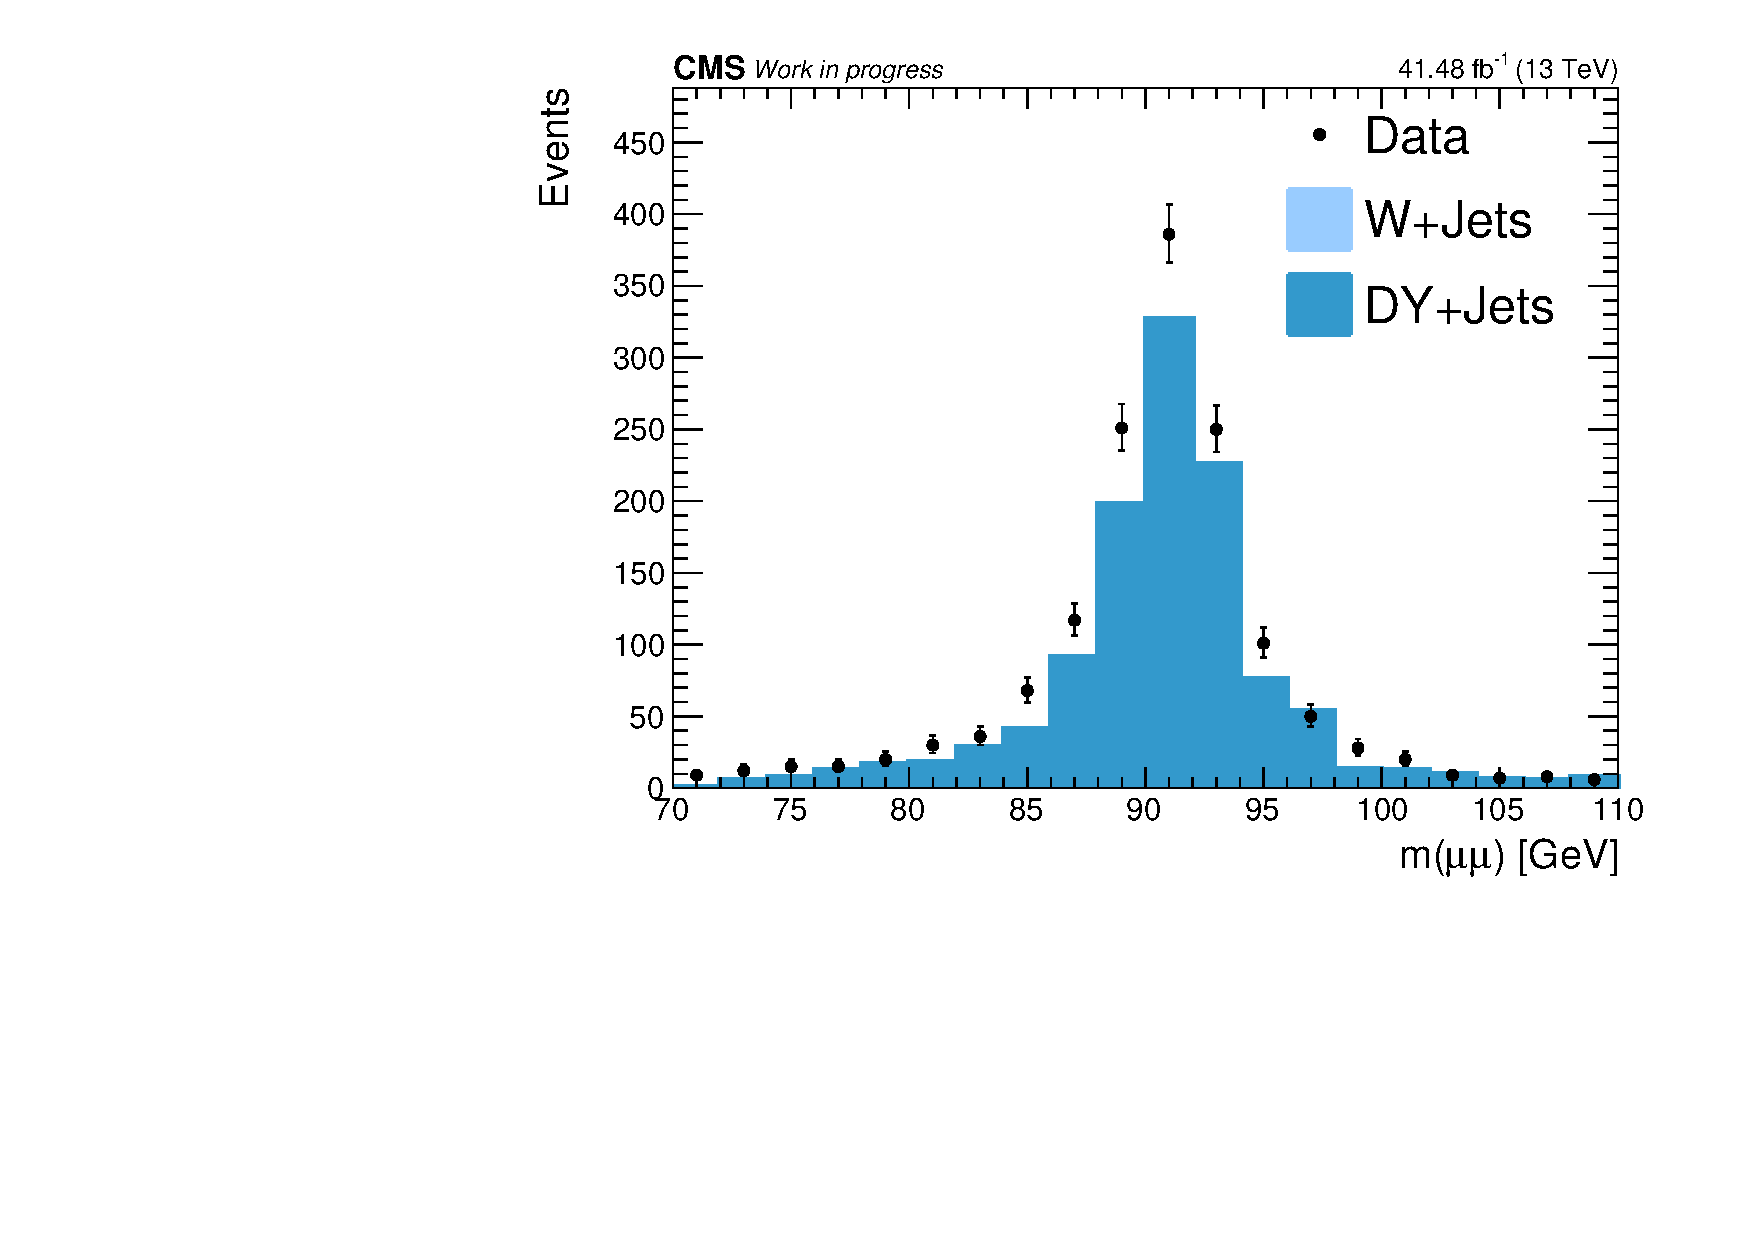
\includegraphics[width=\linewidth]{figs/05_analysis/2017_ZX_Z_mass_MU_postFSR_med.pdf} &
		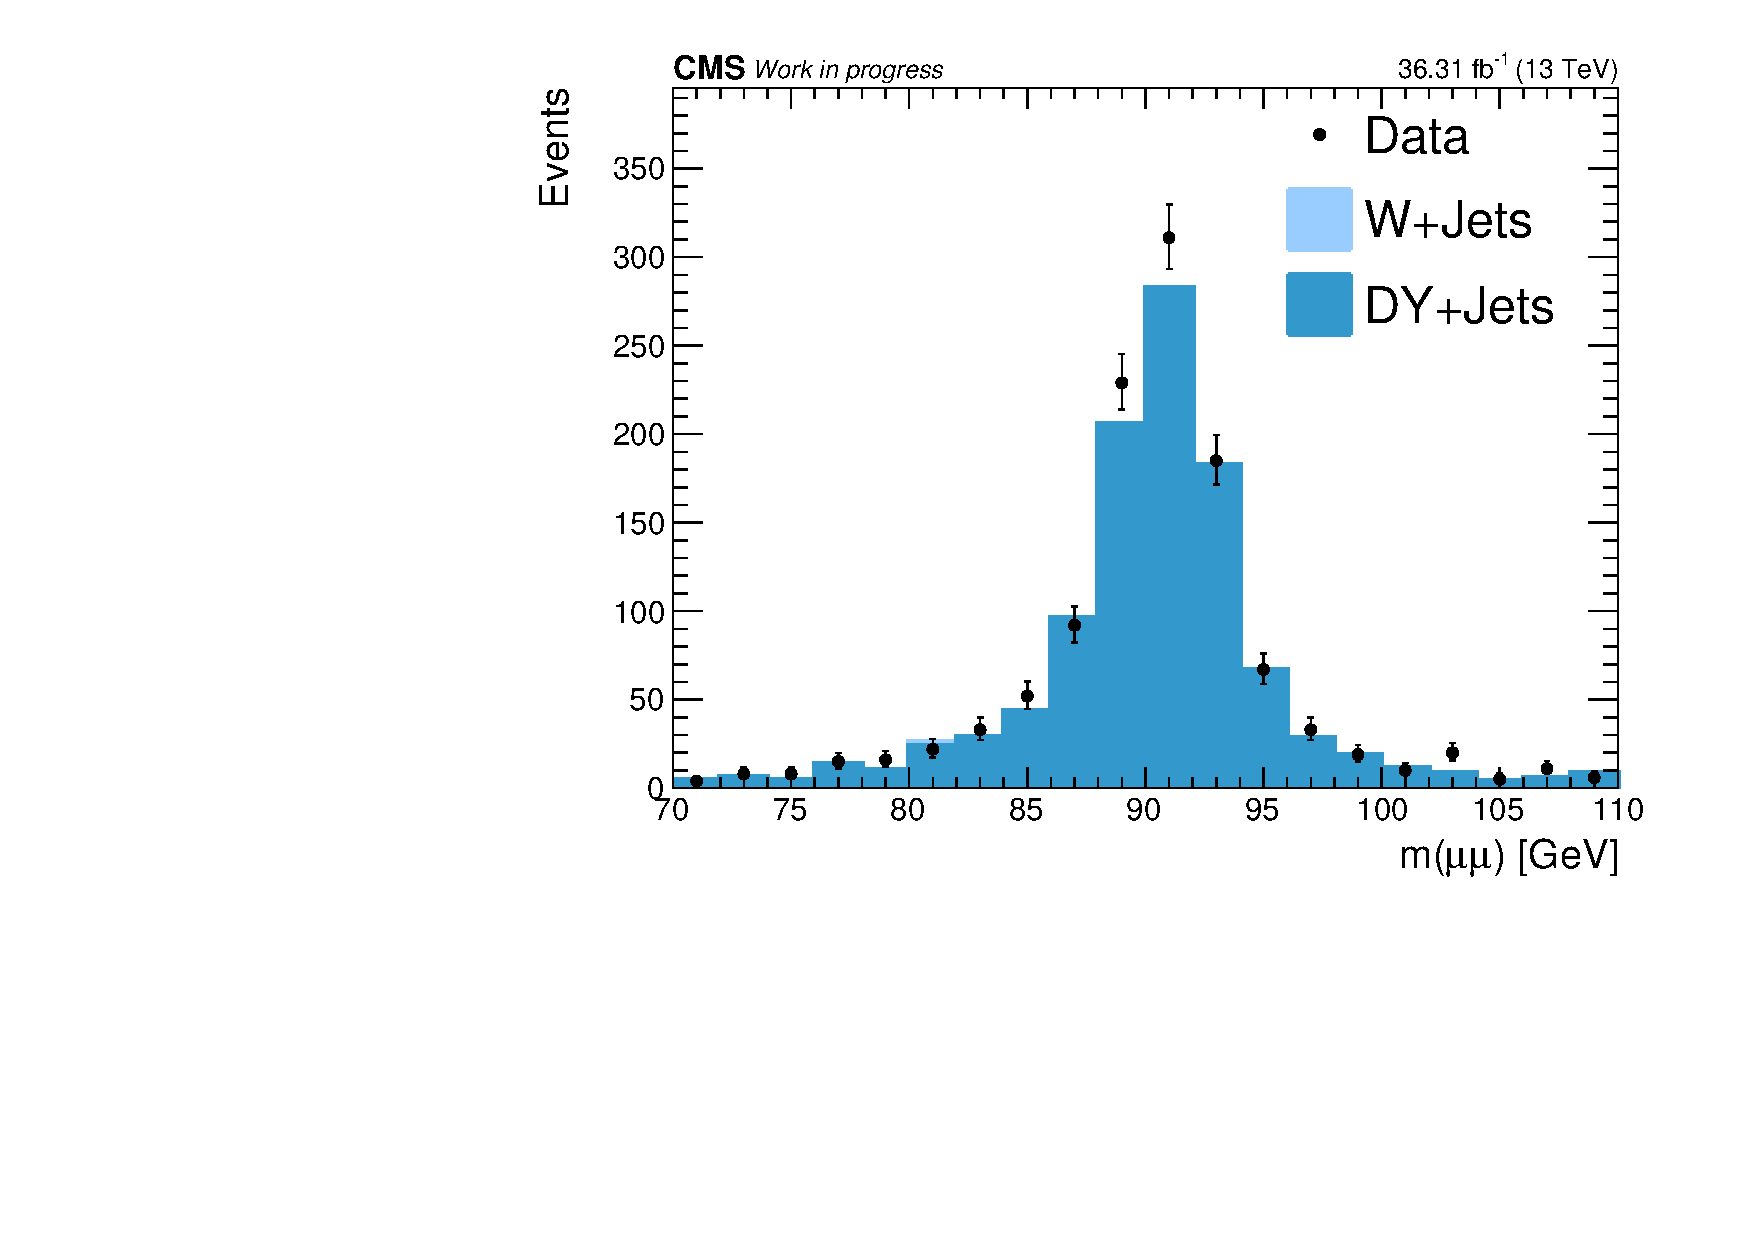
\includegraphics[width=\linewidth]{figs/05_analysis/2016_ZX_Z_mass_MU_postFSR_med.pdf} \\
		2018 $\PZ\to\Pe\Pe$ & 2017 $\PZ\to\Pe\Pe$ & 2016 $\PZ\to\Pe\Pe$\\
		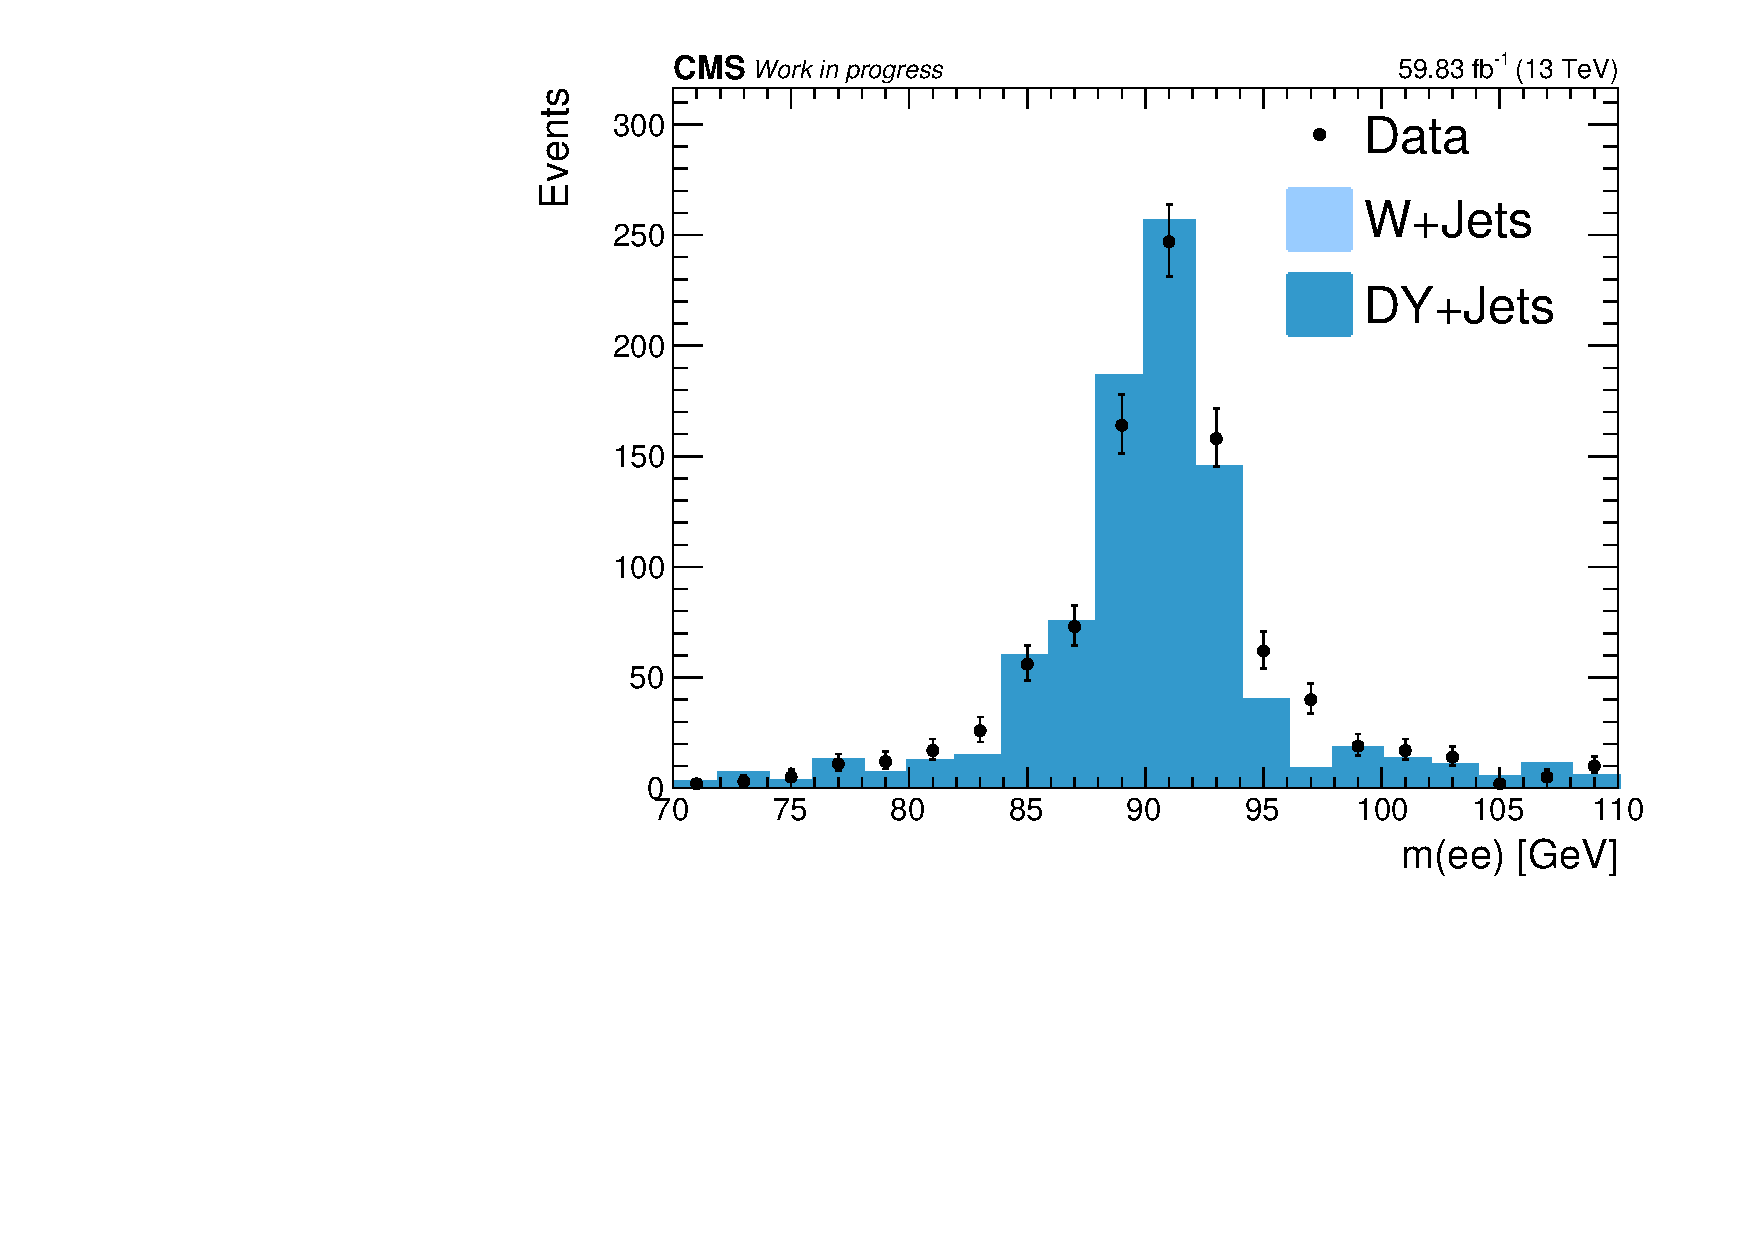
\includegraphics[width=\linewidth]{figs/05_analysis/2018_ZX_Z_mass_ELE_postFSR_med.pdf} &
		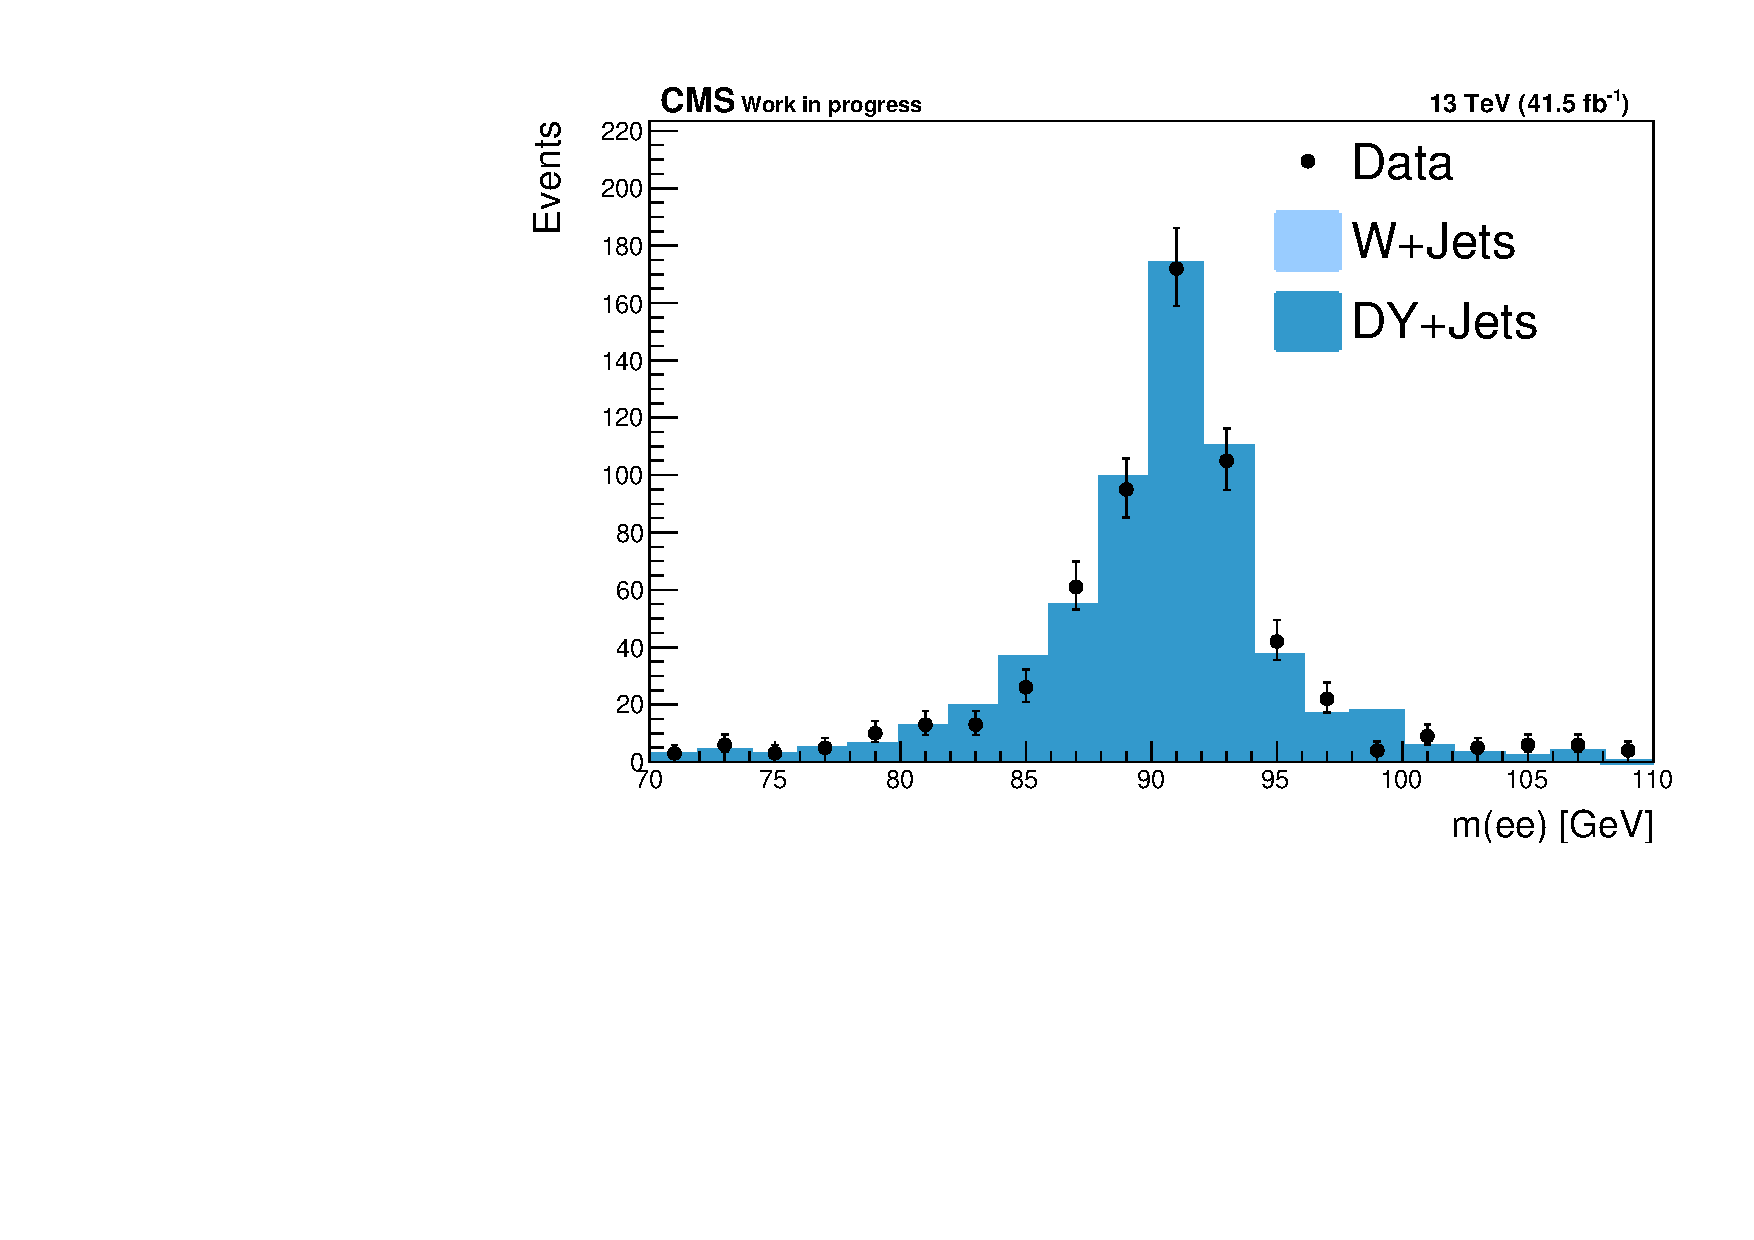
\includegraphics[width=\linewidth]{figs/05_analysis/2017_ZX_Z_mass_ELE_postFSR_med.pdf} &
		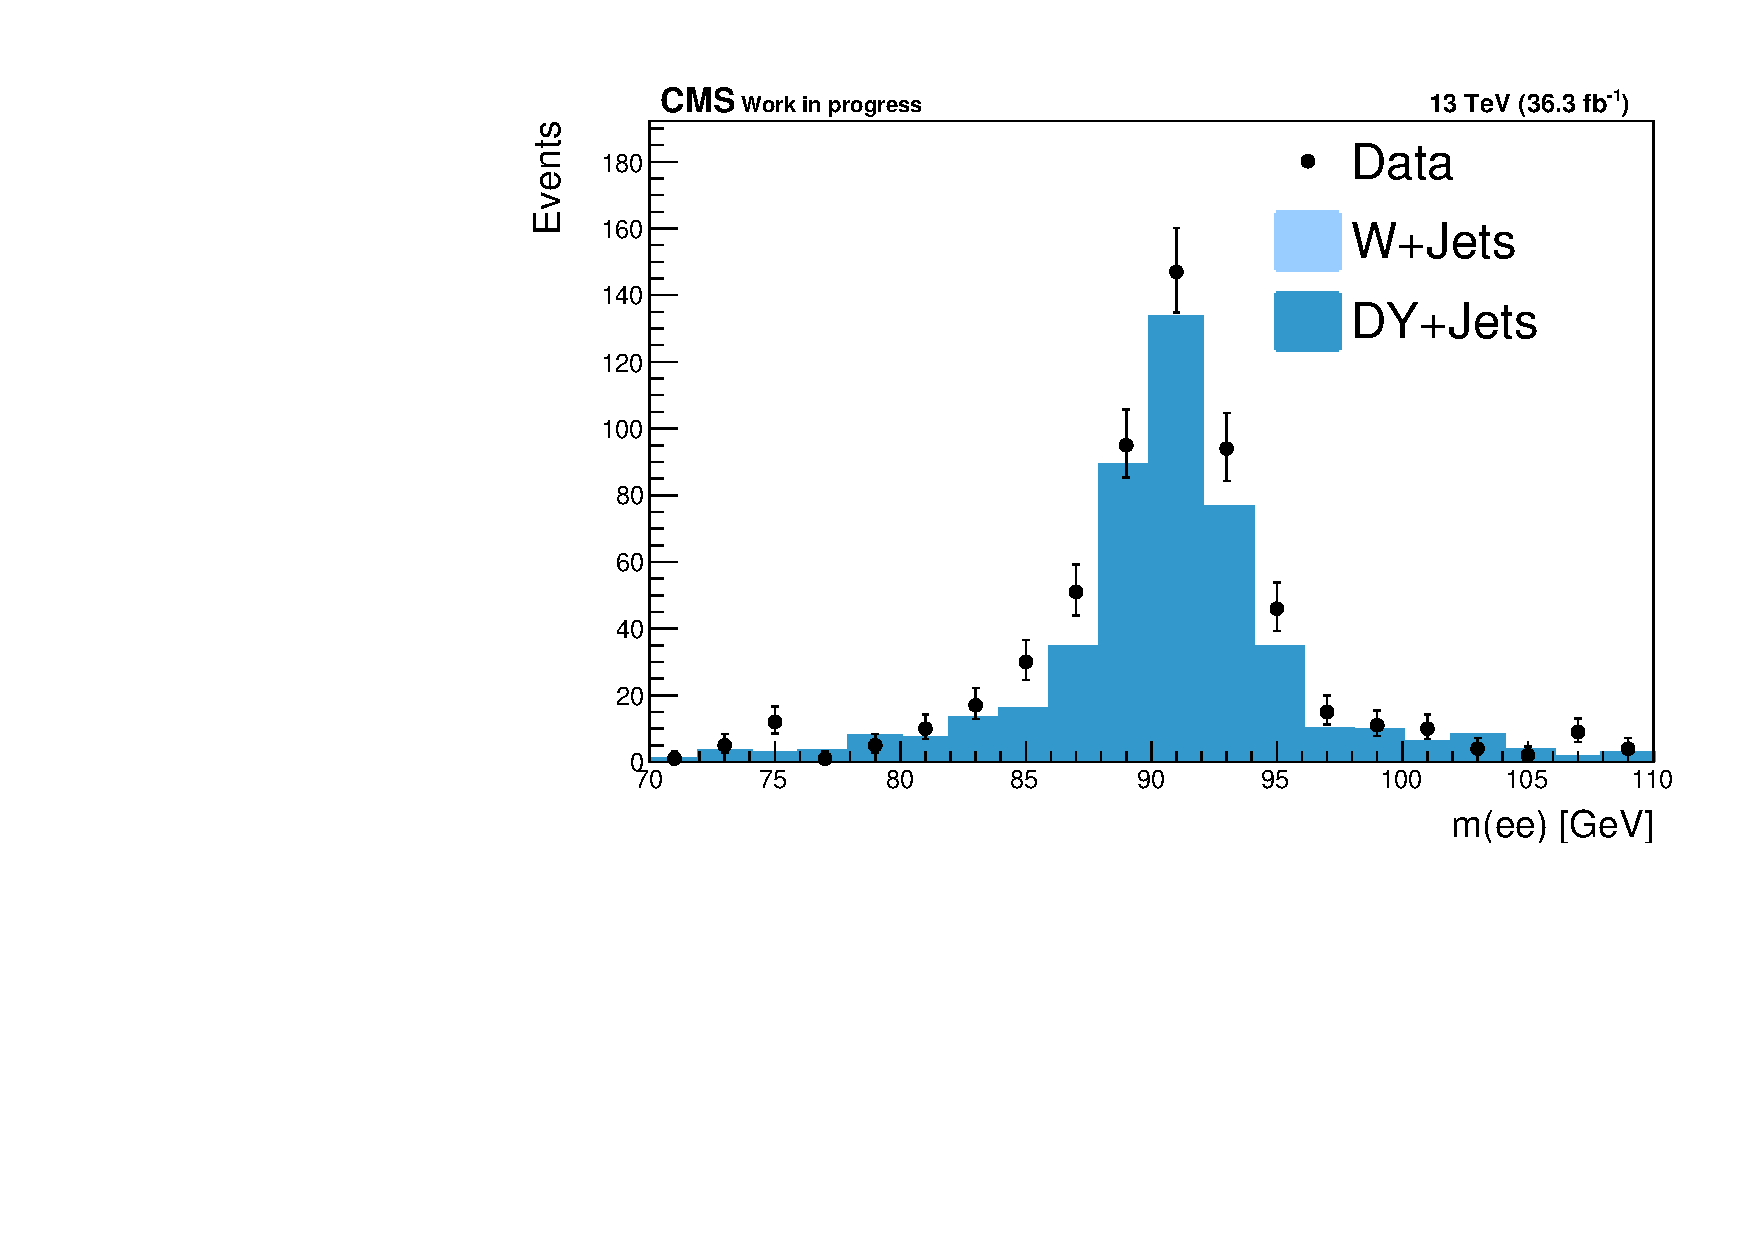
\includegraphics[width=\linewidth]{figs/05_analysis/2016_ZX_Z_mass_ELE_postFSR_med.pdf} \\
	\end{tabular}
	\caption[m$\left(\ell^+\ell^-\right)$ data and simulated background after rejecting FSR events across all years in the anti-ID control region.]{m$\left(\ell^+\ell^-\right)$ data and simulated background after rejecting FSR events across all years in the anti-ID control region. Top row: $\PZ\to\PGm\PGm$ category. Bottom row: $\PZ\to\Pe\Pe$ category}
	\label{fig:zmass_postFSR_med}
\end{figure}
\begin{figure}[htb!]
	\begin{tabular}{>{\centering\arraybackslash}m{0.32\linewidth} >{\centering\arraybackslash}m{0.32\linewidth} >{\centering\arraybackslash}m{0.32\linewidth}}
		2018 $\PZ\to\PGm\PGm$ & 2017 $\PZ\to\PGm\PGm$ & 2016 $\PZ\to\PGm\PGm$\\		
		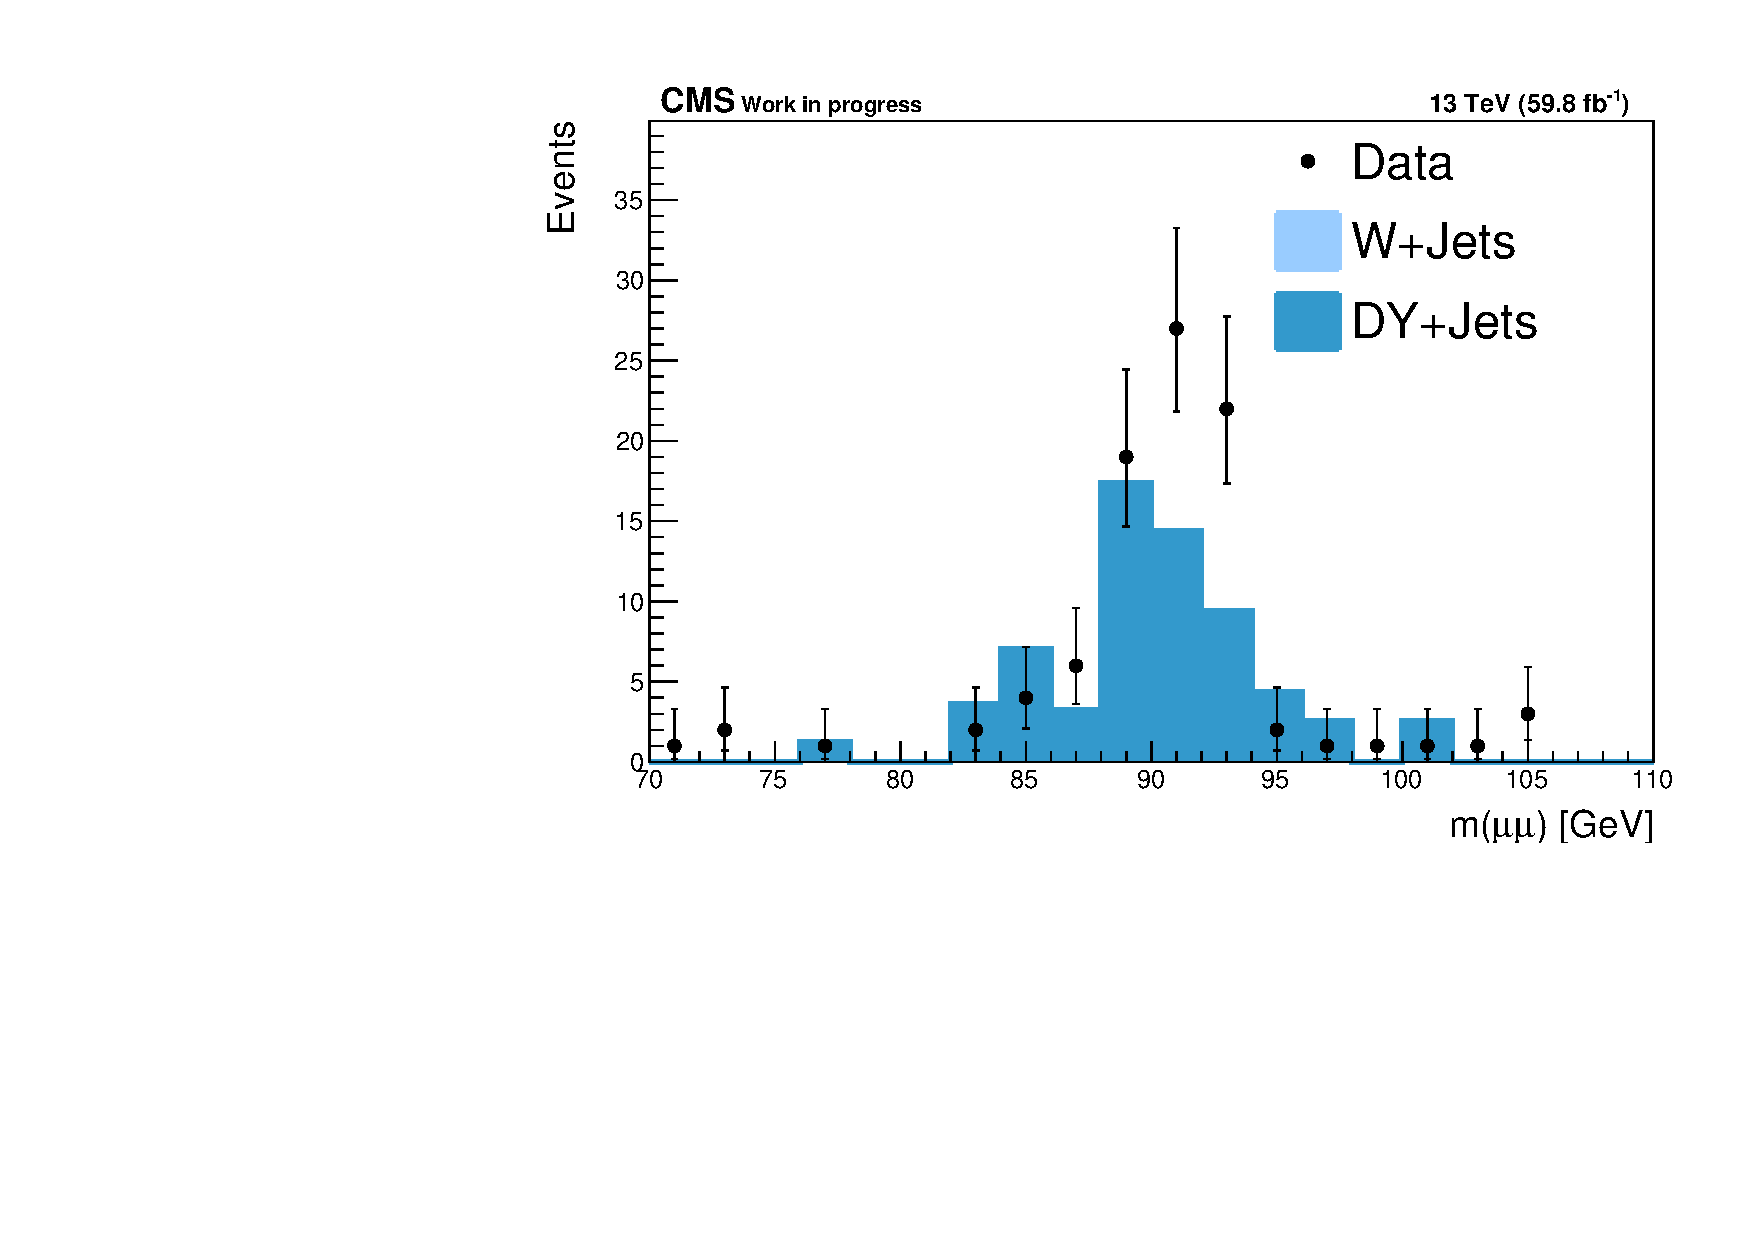
\includegraphics[width=\linewidth]{figs/05_analysis/2018_ZX_Z_mass_MU_postFSR_tight.pdf} &
		\includegraphics[width=\linewidth]{figs/05_analysis/2017_ZX_Z_mass_MU_postFSR_tight.pdf} &
		\includegraphics[width=\linewidth]{figs/05_analysis/2016_ZX_Z_mass_MU_postFSR_tight.pdf} \\
		2018 $\PZ\to\Pe\Pe$ & 2017 $\PZ\to\Pe\Pe$ & 2016 $\PZ\to\Pe\Pe$\\		
		\includegraphics[width=\linewidth]{figs/05_analysis/2018_ZX_Z_mass_ELE_postFSR_tight.pdf} &
		\includegraphics[width=\linewidth]{figs/05_analysis/2017_ZX_Z_mass_ELE_postFSR_tight.pdf} &
		\includegraphics[width=\linewidth]{figs/05_analysis/2016_ZX_Z_mass_ELE_postFSR_tight.pdf} \\
	\end{tabular}
	\caption[m$\left(\ell^+\ell^-\right)$ data and simulated background after rejecting FSR events across all years in the ID signal region.]{m$\left(\ell^+\ell^-\right)$ data and simulated background after rejecting FSR events across all years in the ID signal region. Top row: $\PZ\to\PGm\PGm$ category. Bottom row: $\PZ\to\Pe\Pe$ category}
	\label{fig:zmass_postFSR_tight}
\end{figure}

\subsubsection{Low \pt Photon Background} \label{sec:ana_photonpt}
Equation~\ref{eq:me1e2theta} shows that, for energetically allowed decays, the angle between two photons increases monotonically as the assumed value of \mphi increases. The position of the ECAL clusters is fixed, so the vertex becomes more displaced as the angle increases, leading to low \pt photon background with large \lxy. This makes the photon \pt a useful handle to discriminate signal and background. We compare the \pt spectrum of leading and sub-leading photons in the anti-ID control region and signal region for events having a positive \lxy in order to determine optimal cut values. As one additional requirement, when comparing the leading \pt spectrum we select background events where $\gamma_1$ is ID'd and $\gamma_2$ is anti-ID'd (and vice versa when plotting the subleading photon). Plots comparing signal and background \pt distributions for leading and subleading photons can be seen in figure~\ref{fig:pt_comparison}.

\begin{figure}[htb!]
	\centering
	\captionsetup[subfigure]{justification=centering}
	\begin{subfigure}[h]{0.45\linewidth}
		\centering
		\includegraphics[width=\linewidth]{figs/05_analysis/2018_ZX_g1_pt_mx20_MU_comp.pdf}
		\caption{$p_\mathrm{T}(\gamma_1)$ for $\mphi=20\GeV$.}
	\end{subfigure}
	\begin{subfigure}[h]{0.45\linewidth}
		\centering
		\includegraphics[width=\linewidth]{figs/05_analysis/2018_ZX_g2_pt_mx20_MU_comp.pdf}
		\caption{$p_\mathrm{T}(\gamma_2)$ for $\mphi=20\GeV$.}
	\end{subfigure}
	\begin{subfigure}[h]{0.45\linewidth}
		\centering
		\includegraphics[width=\linewidth]{figs/05_analysis/2018_ZX_g1_pt_mx50_MU_comp.pdf}
		\caption{$p_\mathrm{T}(\gamma_2)$ for $\mphi=50\GeV$.}
	\end{subfigure}
	\begin{subfigure}[h]{0.45\linewidth}
		\centering
		\includegraphics[width=\linewidth]{figs/05_analysis/2018_ZX_g2_pt_mx50_MU_comp.pdf}
		\caption{$p_\mathrm{T}(\gamma_2)$ for $\mphi=50\GeV$.}
	\end{subfigure}
	\caption[Comparison of leading and subleading photon \pt in the anti-ID control region and signal region for the $\PZ\to\PGm\PGm$ category under the assumptions $\mphi=20\GeV$ (top) and $\mphi=50\GeV$ (bottom).]{Comparison of leading and subleading photon \pt in the anti-ID control region and signal region for the $\PZ\to\PGm\PGm$ category under the assumptions $\mphi=20\GeV$ (top) and $\mphi=50\GeV$ (bottom).}
	\label{fig:pt_comparison}
\end{figure}

The final cuts were chosen to be $p_\mathrm{T}(\gamma_1)>35\GeV$ and $p_\mathrm{T}(\gamma_2)>25\GeV$. These cuts reject between 70-80\% of background and maintain about 70\% signal efficiency. The exact values for background rejection can be seen in table~\ref{tab:cuts_pt}, while the cut efficiency for signal can be seen in figure~\ref{fig:signal_acceptance}.

\begin{table}[htb!]
	\begin{center}
		\caption[Photon \pt cut efficiency on control region background]{Photon \pt cut efficiency on control region background}
		\label{tab:cuts_pt}
		\begin{tabular}{l|l|l}
			\hline
			m$_{\Phi}$ [GeV] & \PZ $\rightarrow \PGm \PGm$  & \PZ $\rightarrow$ ee\\
			\hline
			15	&	.24	&	.23 \\	
			\hline
			20	&	.27	&	.33 \\
			\hline
			30	&	.27	&	.26 \\
			\hline
			40	&	.29	&	.28 \\
			\hline
			50	&	.29	&	.28 \\
			\hline
			55	&	.30	&	.30 \\
			\hline
		\end{tabular}
	\end{center}
\end{table}

\subsubsection{Final Selection Requirements} \label{sec:ana_final_selection}
The final \lxy agnostic data and Monte Carlo comparison plots after applying the FSR and tight photon \pt cuts can be seen in figures~\ref{fig:zmass_final_med}$\,$-$\,$\ref{fig:zmass_final_tight}. Signal Monte Carlo distributions from the $\mphi=30\GeV$, $c\tau=0\unit{mm}$ samples are overlaid at arbitrary normalization for shape comparison. In the ID signal region, the Monte Carlo background shows poor agreement with data and consists of very few weighted events with limited statistical power. For this reason we opt for a data driven method for background estimation.

\begin{figure}[htb!]
	\begin{tabular}{>{\centering\arraybackslash}m{0.32\linewidth} >{\centering\arraybackslash}m{0.32\linewidth} >{\centering\arraybackslash}m{0.32\linewidth}}
		2018 & 2017 & 2016\\
		\includegraphics[width=\linewidth]{figs/05_analysis/2018_ZX_Z_mass_MU_final_loose.pdf} & 
		\includegraphics[width=\linewidth]{figs/05_analysis/2017_ZX_Z_mass_MU_final_loose.pdf} & 
		\includegraphics[width=\linewidth]{figs/05_analysis/2016_ZX_Z_mass_MU_final_loose.pdf} \\
		anti-ID $\PZ\to\PGm\PGm$ & anti-ID $\PZ\to\PGm\PGm$ & anti-ID $\PZ\to\PGm\PGm$\\
		\includegraphics[width=\linewidth]{figs/05_analysis/2018_ZX_Z_mass_ELE_final_loose.pdf} & 
		\includegraphics[width=\linewidth]{figs/05_analysis/2017_ZX_Z_mass_ELE_final_loose.pdf} & 
		\includegraphics[width=\linewidth]{figs/05_analysis/2016_ZX_Z_mass_ELE_final_loose.pdf} \\
		anti-ID $\PZ\to\Pe\Pe$ & anti-ID $\PZ\to\Pe\Pe$ & anti-ID $\PZ\to\Pe\Pe$\\
	\end{tabular}
	\caption[Final m$\left(\ell^+\ell^-\right)$ distributions for data and simulated samples in the anti-ID control region. Top row: $\PZ\to\PGm\PGm$ category. Bottom row: $\PZ\to\Pe\Pe$ category.]{Final m$\left(\ell^+\ell^-\right)$ distributions for data and simulated samples in the anti-ID control region. Top row: $\PZ\to\PGm\PGm$ category. Bottom row: $\PZ\to\Pe\Pe$ category.}
	\label{fig:zmass_final_med}
\end{figure}

\begin{figure}[htb!]
	\begin{tabular}{>{\centering\arraybackslash}m{0.32\linewidth} >{\centering\arraybackslash}m{0.32\linewidth} >{\centering\arraybackslash}m{0.32\linewidth}}
		2018 & 2017 & 2016\\
		\includegraphics[width=\linewidth]{figs/05_analysis/2018_ZX_Z_mass_MU_final_tight.pdf} & 
		\includegraphics[width=\linewidth]{figs/05_analysis/2017_ZX_Z_mass_MU_final_tight.pdf} & 
		\includegraphics[width=\linewidth]{figs/05_analysis/2016_ZX_Z_mass_MU_final_tight.pdf} \\
		ID $\PZ\to\PGm\PGm$ & ID $\PZ\to\PGm\PGm$ & ID $\PZ\to\PGm\PGm$\\
		\includegraphics[width=\linewidth]{figs/05_analysis/2018_ZX_Z_mass_ELE_final_tight.pdf} & 
		\includegraphics[width=\linewidth]{figs/05_analysis/2017_ZX_Z_mass_ELE_final_tight.pdf} & 
		\includegraphics[width=\linewidth]{figs/05_analysis/2016_ZX_Z_mass_ELE_final_tight.pdf} \\
		ID $\PZ\to\Pe\Pe$ & ID $\PZ\to\Pe\Pe$ & ID $\PZ\to\Pe\Pe$\\
	\end{tabular}
	\caption[Final m$\left(\ell^+\ell^-\right)$ distributions for data and simulated samples in the ID signal region. Top row: $\PZ\to\PGm\PGm$ category. Bottom row: $\PZ\to\Pe\Pe$ category.]{Final m$\left(\ell^+\ell^-\right)$ distributions for data and simulated samples in the ID signal region. Top row: $\PZ\to\PGm\PGm$ category. Bottom row: $\PZ\to\Pe\Pe$ category.}
	\label{fig:zmass_final_tight}
\end{figure}

The efficiencies and expected yields for simulated background are shown in table~\ref{tab:cuts_bkg}. For signal samples we plot the acceptances as an efficiency relative to the total number of generated events for all masses and lifetimes, separating two photon events where only one $\Phi$ decays to photons and four final state photon events where both $\Phi$ decay to photons. The HLT and object preselection cuts are applied as described in sections~\ref{sec:ana_triggers} and~\ref{sec:ana_preselection}. The FSR rejection cuts are applied, but due to the high signal efficiency the points overlap with the previous cuts on loose cut based ID. The positive \lxy cuts result in a decrease in efficiency in the four photon categories due to mispaired photons, where one photon from each $\Phi$ is chosen to calculate the vertex. The full set of signal efficiency plots are shown in figure~\ref{fig:signal_acceptance}.

\begin{table}[htb!]
	\begin{center}
		\caption[Cutflow table and expected yields on background Monte Carlo in the ID+ID signal region]{Cutflow table and expected yields on background Monte Carlo in the ID+ID signal region}
		\label{tab:cuts_bkg}
		\begin{tabular}{l|l|l}
			& \multicolumn{2}{l}{Simulated Events}\\
			\hline
			Selection & \PZ $\rightarrow \PGm \PGm$  & \PZ $\rightarrow$ ee\\
			\hline
			\hline
			Initial (from preselection) & 67.4 & 22.1 \\
			\hline
			Final State Radiation & 64.7 & 13.6\\
			\hline
			$\pt(\gamma_1)>35 \text{GeV}, \pt(\gamma_2)>25 \text{GeV}$ & 28.0 & 5.5 \\
			\hline
			\hline
			Total Background Rejection & 59\% & 75\%\\
			\hline
		\end{tabular}
	\end{center}
\end{table}

\begin{figure}[htb!]
	\centering
	\captionsetup[subfigure]{justification=centering}
	\begin{subfigure}[h]{0.49\linewidth}
		\centering
		\includegraphics[width=\linewidth]{figs/05_analysis/2018_signal_2G2Q_Z_MU_efficiency_raw.pdf}
		\caption{$\PZ\to\PGm\PGm$ in the 2$\gamma$ category.}
	\end{subfigure}
	\begin{subfigure}[h]{0.49\linewidth}
		\centering
		\includegraphics[width=\linewidth]{figs/05_analysis/2018_signal_2G2Q_Z_ELE_efficiency_raw.pdf}
		\caption{$\PZ\to\Pe\Pe$ in the 2$\gamma$ category.}
	\end{subfigure}
	\begin{subfigure}[h]{0.49\linewidth}
		\centering
		\includegraphics[width=\linewidth]{figs/05_analysis/2018_signal_4G_Z_MU_efficiency_raw.pdf}
		\caption{$\PZ\to\PGm\PGm$ in the 4$\gamma$ category.}
	\end{subfigure}
	\begin{subfigure}[h]{0.49\linewidth}
		\centering
		\includegraphics[width=\linewidth]{figs/05_analysis/2018_signal_4G_Z_ELE_efficiency_raw.pdf}
		\caption{$\PZ\to\Pe\Pe$ in the 4$\gamma$ category.}
	\end{subfigure}
	\caption[Cutflow efficiency for signal events with exactly 2 photons (top) and 4 photons (bottom).]{Cutflow efficiency for signal events with exactly 2 photons (top) and 4 photons (bottom).}
	\label{fig:signal_acceptance}
\end{figure}


\section{Background Estimation} \label{sec:ana_bkg}
The limited statistics in the simulated background samples demand a data-driven method of background estimation. As the statistical estimator used to extract signal involves the \lxy distribution in the positive \lxy signal region, it is crucial to get an accurate estimate of both the yield and shape of the expected background. This section outlines the expected sources of background and the process used to estimate the background using the anti-ID control region and negative \lxy sidebands. We demonstrate closure tests which are used to derive the systematic uncertainties on the background estimation.

\subsection{Sources of Standard Model Background} \label{sec:ana_bkgsources}
There are two main expected SM background contributions originating from the Drell-Yan process, which correspond to combinations of ``fake'' photons from electromagnetic fluctuations of neutral pions produced in jets or PU, and ``real'' photons from initial or final state radiation (ISR/FSR). The FSR photons are strongly reducible using invariant mass cuts outlined in section~\ref{sec:ana_fsr}. From studies using generator level information it was determined that the subleading photons primarily originate from jets. A Feynman diagram showing possible sources of background is shown in figure~\ref{fig:bkg_dyjets}.

\begin{figure}[htb!]
	\centering
	% !TEX = root = ../../thesis.tex
\begin{tikzpicture}
	\begin{feynman}
		% Defining vertex coordinates since \feynmandiagram automatic vertices command needs lualatex to work and I can't figure out how
		\coordinate[label=left:$q$] (i1) at (-3.5, 2); %Initial q
		\coordinate[label=left:$\bar{q}$] (i2) at (-3.5,-2); %Initial qbar
		\coordinate (v1) at (-1.5, 0); %photon vertex 1
		\coordinate (v2) at (1.5, 0);  %photon vertex 2
		\coordinate[label=right:$\ell$] (f1) at (3.5, 2);  %final lepton 1
		\coordinate[label=right:$\bar{\ell}$] (f2) at (3.5, -2); %final lepton 2
		\coordinate (g1) at (-2.5, 1); %gluon vertex 1
		\coordinate (g2) at (-1.5, 1.5); %gluon vertex 2
		\coordinate (q1) at (-.5, 1.75); %pi0 q1
		\coordinate (q2) at (-.5, 1.25); %pi0 q2
		\coordinate (isr1) at (-2.5, -1); %isr v1
		\coordinate[label=right:$\gamma$] (isr2) at (-1.5, -1.5); %isr v2
		\coordinate (fsr1) at (2.5, -1);
		\coordinate[label=right:$\gamma$] (fsr2) at (3.5, -.5);
		
		% Drawing everything
		\draw[fermion] (i1) -- (v1);
		\draw[fermion] (v1) -- (i2);
		\draw[photon] (v1) -- (v2);
		\draw[fermion] (f2) -- (v2);
		\draw[fermion] (v2) -- (f1);
		\draw[gluon] (g1) -- (g2);
		\draw[fermion] (g2) -- (q1);
		\draw[fermion] (q2) -- (g2);
		\draw[photon] (isr1) -- (isr2);
		\draw[photon] (fsr1) -- (fsr2);
		
		% Extra labels
		\draw[black, decorate, decoration={brace, amplitude=.65ex, raise=1ex}] (-.5, 1.75) -- (-.5, 1.25);
		\node[label={right:$\pi^0$}] at (-.43, 1.55){};
		
		\node[label={below:$Z/\gamma^*$}] at (0, 0){};
		
	\end{feynman}
\end{tikzpicture}
	\caption[Feynman diagram showing the possible background contributions from Drell-Yan events. Photons can originate from neutral pions produced in jets, initial state radiation from quarks, or final state radiation from leptons.]{Feynman diagram showing the possible background contributions from Drell-Yan events. Photons can originate from neutral pions produced in jets, initial state radiation from quarks, or final state radiation from leptons.}
	\label{fig:bkg_dyjets}
\end{figure}

There are zero sources of resonant diphoton background expected in this analysis. While the standard model process $\PH\to\gamma\gamma$ produces two final state photons, we expect very few events due to the low branching fraction of 0.0025~\cite{Workman:2022ynf}. For the few events that pass full selection criteria, the invariant diphoton mass of $\mgg=\mh=125\GeV$ would classify events in the negative \lxy sideband by section~\ref{sec:ana_vertex}. This region is used to determine the yield of the expected background and would result in a negligible overestimation of background events.

\subsection{Method of Background Estimation} \label{sec:ana_bkgest}
The largest obstacle towards implementing a reliable background estimation for this analysis was the large statistical fluctuations of the estimated contributions using weights of events in both adjoint regions (e.g. fake-rate based method) and simulation. In order to account for the correlation between photon kinematics, we predict the shape of the \lxy and \mgg distributions using the anti-ID control region, and normalize the expected number of background events by scaling the anti-ID control region to match the yield of the ID signal region in the negative \lxy sideband. The estimated background in bin $i$ is given by
\begin{equation}
	\label{eq:background}
	N_{\mathrm{bkg}}^{i} = \frac{N(\gamma_\mathrm{ID}+\gamma_\mathrm{ID}, \mgg > \mh/2)}{N(\gamma_\mathrm{ID}+\gamma_\mathrm{antiID}, \mgg > \mh/2)}\times N(\gamma_\mathrm{ID}+\gamma_\mathrm{antiID}, i)
\end{equation}

Where $N(\gamma_\mathrm{ID}+\gamma_\mathrm{(anti)ID}, \mgg > \mh/2)$ is the number of events in the \lxy sideband of the (anti)ID region and $N(\gamma_\mathrm{ID}+\gamma_\mathrm{antiID}, i)$ is the number of events in bin $i$ of the anti-ID control region. 

\subsection{Closure Tests} \label{sec:ana_bkgclosure}
The method of background estimation is validated by comparing the shape of the negative \lxy sidebands in both the ID signal region and anti-ID control region. The behavior of the fit as \lxy approaches zero is used as an indicator for the agreement in the positive \lxy region, and is used to determine the bin-by-bin shape uncertainty. Error bars for the signal and control region data represent the $68\%$ Poisson confidence interval given by
\begin{equation}
	\text{C.I.}=\left[0.5*\chi^2(2N, \alpha/2),\, 0.5*\chi^2(2(N+1), 1-\alpha/2)\right]
\end{equation}
where $\chi^2$ is the chi-square critical value, N is the number of observed events, and $\alpha$ is the significance level of $(1-0.68)$. Since the anti-ID bin contents are scaled in order to match the yield of the ID signal region, the uncertainty is scaled by the same amount.

The anti-ID control region shows compatible values with the ID signal region across all ranges of negative \lxy. Based on the disagreement as \lxy approaches 0, we apply a conservative 40\% uncertainty on each bin in the positive \lxy signal region. The full set of closure plots across all categories for each year can be seen in figures~\ref{fig:bkg_m15}-\ref{fig:bkg_m55}.

\begin{figure}[htb!]
	\centering
	\begin{tabular}{>{\centering\arraybackslash}m{0.45\linewidth} >{\centering\arraybackslash}m{0.45\linewidth}}
		2018 $\PZ\to\PGm\PGm$ & 2018 $\PZ\to\Pe\Pe$\\
		\includegraphics[width=0.75\linewidth]{figs/05_analysis/closure_ZH_MU_m15_sideband_2018.pdf} &
		\includegraphics[width=0.75\linewidth]{figs/05_analysis/closure_ZH_ELE_m15_sideband_2018.pdf} \\
		2017 $\PZ\to\PGm\PGm$ & 2017 $\PZ\to\Pe\Pe$\\
		\includegraphics[width=0.75\linewidth]{figs/05_analysis/closure_ZH_MU_m15_sideband_2017.pdf} &
		\includegraphics[width=0.75\linewidth]{figs/05_analysis/closure_ZH_ELE_m15_sideband_2017.pdf} \\
		2016 $\PZ\to\PGm\PGm$ & 2016 $\PZ\to\Pe\Pe$\\
		\includegraphics[width=0.75\linewidth]{figs/05_analysis/closure_ZH_MU_m15_sideband_2016.pdf} &
		\includegraphics[width=0.75\linewidth]{figs/05_analysis/closure_ZH_ELE_m15_sideband_2016.pdf} \\
	\end{tabular}
	\caption[Shape comparison of ID signal region and anti-ID control region data in the negative \lxy sideband for $\mphi=15\GeV$ in the $\PZ\to\PGm\PGm$ category (left) and $\PZ\to\Pe\Pe$ category (bottom) across all three years.]{Shape comparison of ID signal region and anti-ID control region data in the negative \lxy sideband for $\mphi=15\GeV$ in the $\PZ\to\PGm\PGm$ category (left) and $\PZ\to\Pe\Pe$ category (bottom) across all three years.}
	\label{fig:bkg_m15}
\end{figure}

\begin{figure}[htb!]
	\centering
	\begin{tabular}{>{\centering\arraybackslash}m{0.45\linewidth} >{\centering\arraybackslash}m{0.45\linewidth}}
		2018 $\PZ\to\PGm\PGm$ & 2018 $\PZ\to\Pe\Pe$\\
		\includegraphics[width=0.75\linewidth]{figs/05_analysis/closure_ZH_MU_m20_sideband_2018.pdf} &
		\includegraphics[width=0.75\linewidth]{figs/05_analysis/closure_ZH_ELE_m20_sideband_2018.pdf} \\
		2017 $\PZ\to\PGm\PGm$ & 2017 $\PZ\to\Pe\Pe$\\
		\includegraphics[width=0.75\linewidth]{figs/05_analysis/closure_ZH_MU_m20_sideband_2017.pdf} &
		\includegraphics[width=0.75\linewidth]{figs/05_analysis/closure_ZH_ELE_m20_sideband_2017.pdf} \\
		2016 $\PZ\to\PGm\PGm$ & 2016 $\PZ\to\Pe\Pe$\\
		\includegraphics[width=0.75\linewidth]{figs/05_analysis/closure_ZH_MU_m20_sideband_2016.pdf} &
		\includegraphics[width=0.75\linewidth]{figs/05_analysis/closure_ZH_ELE_m20_sideband_2016.pdf} \\
	\end{tabular}
	\caption[Shape comparison of ID signal region and anti-ID control region data in the negative \lxy sideband for $\mphi=20\GeV$ in the $\PZ\to\PGm\PGm$ category (left) and $\PZ\to\Pe\Pe$ category (bottom) across all three years.]{Shape comparison of ID signal region and anti-ID control region data in the negative \lxy sideband for $\mphi=20\GeV$ in the $\PZ\to\PGm\PGm$ category (left) and $\PZ\to\Pe\Pe$ category (bottom) across all three years.}
	\label{fig:bkg_m20}
\end{figure}

\begin{figure}[htb!]
	\centering
	\begin{tabular}{>{\centering\arraybackslash}m{0.45\linewidth} >{\centering\arraybackslash}m{0.45\linewidth}}
		2018 $\PZ\to\PGm\PGm$ & 2018 $\PZ\to\Pe\Pe$\\
		\includegraphics[width=0.75\linewidth]{figs/05_analysis/closure_ZH_MU_m30_sideband_2018.pdf} &
		\includegraphics[width=0.75\linewidth]{figs/05_analysis/closure_ZH_ELE_m30_sideband_2018.pdf} \\
		2017 $\PZ\to\PGm\PGm$ & 2017 $\PZ\to\Pe\Pe$\\
		\includegraphics[width=0.75\linewidth]{figs/05_analysis/closure_ZH_MU_m30_sideband_2017.pdf} &
		\includegraphics[width=0.75\linewidth]{figs/05_analysis/closure_ZH_ELE_m30_sideband_2017.pdf} \\
		2016 $\PZ\to\PGm\PGm$ & 2016 $\PZ\to\Pe\Pe$\\
		\includegraphics[width=0.75\linewidth]{figs/05_analysis/closure_ZH_MU_m30_sideband_2016.pdf} &
		\includegraphics[width=0.75\linewidth]{figs/05_analysis/closure_ZH_ELE_m30_sideband_2016.pdf} \\
	\end{tabular}
	\caption[Shape comparison of ID signal region and anti-ID control region data in the negative \lxy sideband for $\mphi=30\GeV$ in the $\PZ\to\PGm\PGm$ category (left) and $\PZ\to\Pe\Pe$ category (bottom) across all three years.]{Shape comparison of ID signal region and anti-ID control region data in the negative \lxy sideband for $\mphi=30\GeV$ in the $\PZ\to\PGm\PGm$ category (left) and $\PZ\to\Pe\Pe$ category (bottom) across all three years.}
	\label{fig:bkg_m30}
\end{figure}

\begin{figure}[htb!]
	\centering
	\begin{tabular}{>{\centering\arraybackslash}m{0.45\linewidth} >{\centering\arraybackslash}m{0.45\linewidth}}
		2018 $\PZ\to\PGm\PGm$ & 2018 $\PZ\to\Pe\Pe$\\
		\includegraphics[width=0.75\linewidth]{figs/05_analysis/closure_ZH_MU_m40_sideband_2018.pdf} &
		\includegraphics[width=0.75\linewidth]{figs/05_analysis/closure_ZH_ELE_m40_sideband_2018.pdf} \\
		2017 $\PZ\to\PGm\PGm$ & 2017 $\PZ\to\Pe\Pe$\\
		\includegraphics[width=0.75\linewidth]{figs/05_analysis/closure_ZH_MU_m40_sideband_2017.pdf} &
		\includegraphics[width=0.75\linewidth]{figs/05_analysis/closure_ZH_ELE_m40_sideband_2017.pdf} \\
		2016 $\PZ\to\PGm\PGm$ & 2016 $\PZ\to\Pe\Pe$\\
		\includegraphics[width=0.75\linewidth]{figs/05_analysis/closure_ZH_MU_m40_sideband_2016.pdf} &
		\includegraphics[width=0.75\linewidth]{figs/05_analysis/closure_ZH_ELE_m40_sideband_2016.pdf} \\
	\end{tabular}
	\caption[Shape comparison of ID signal region and anti-ID control region data in the negative \lxy sideband for $\mphi=40\GeV$ in the $\PZ\to\PGm\PGm$ category (left) and $\PZ\to\Pe\Pe$ category (bottom) across all three years.]{Shape comparison of ID signal region and anti-ID control region data in the negative \lxy sideband for $\mphi=40\GeV$ in the $\PZ\to\PGm\PGm$ category (left) and $\PZ\to\Pe\Pe$ category (bottom) across all three years.}
	\label{fig:bkg_m40}
\end{figure}

\begin{figure}[htb!]
	\centering
	\begin{tabular}{>{\centering\arraybackslash}m{0.45\linewidth} >{\centering\arraybackslash}m{0.45\linewidth}}
		2018 $\PZ\to\PGm\PGm$ & 2018 $\PZ\to\Pe\Pe$\\
		\includegraphics[width=0.75\linewidth]{figs/05_analysis/closure_ZH_MU_m50_sideband_2018.pdf} &
		\includegraphics[width=0.75\linewidth]{figs/05_analysis/closure_ZH_ELE_m50_sideband_2018.pdf} \\
		2017 $\PZ\to\PGm\PGm$ & 2017 $\PZ\to\Pe\Pe$\\
		\includegraphics[width=0.75\linewidth]{figs/05_analysis/closure_ZH_MU_m50_sideband_2017.pdf} &
		\includegraphics[width=0.75\linewidth]{figs/05_analysis/closure_ZH_ELE_m50_sideband_2017.pdf} \\
		2016 $\PZ\to\PGm\PGm$ & 2016 $\PZ\to\Pe\Pe$\\
		\includegraphics[width=0.75\linewidth]{figs/05_analysis/closure_ZH_MU_m50_sideband_2016.pdf} &
		\includegraphics[width=0.75\linewidth]{figs/05_analysis/closure_ZH_ELE_m50_sideband_2016.pdf} \\
	\end{tabular}
	\caption[Shape comparison of ID signal region and anti-ID control region data in the negative \lxy sideband for $\mphi=50\GeV$ in the $\PZ\to\PGm\PGm$ category (left) and $\PZ\to\Pe\Pe$ category (bottom) across all three years.]{Shape comparison of ID signal region and anti-ID control region data in the negative \lxy sideband for $\mphi=50\GeV$ in the $\PZ\to\PGm\PGm$ category (left) and $\PZ\to\Pe\Pe$ category (bottom) across all three years.}
	\label{fig:bkg_m50}
\end{figure}

\begin{figure}[htb!]
	\centering
	\begin{tabular}{>{\centering\arraybackslash}m{0.45\linewidth} >{\centering\arraybackslash}m{0.45\linewidth}}
		2018 $\PZ\to\PGm\PGm$ & 2018 $\PZ\to\Pe\Pe$\\
		\includegraphics[width=0.75\linewidth]{figs/05_analysis/closure_ZH_MU_m55_sideband_2018.pdf} &
		\includegraphics[width=0.75\linewidth]{figs/05_analysis/closure_ZH_ELE_m55_sideband_2018.pdf} \\
		2017 $\PZ\to\PGm\PGm$ & 2017 $\PZ\to\Pe\Pe$\\
		\includegraphics[width=0.75\linewidth]{figs/05_analysis/closure_ZH_MU_m55_sideband_2017.pdf} &
		\includegraphics[width=0.75\linewidth]{figs/05_analysis/closure_ZH_ELE_m55_sideband_2017.pdf} \\
		2016 $\PZ\to\PGm\PGm$ & 2016 $\PZ\to\Pe\Pe$\\
		\includegraphics[width=0.75\linewidth]{figs/05_analysis/closure_ZH_MU_m55_sideband_2016.pdf} &
		\includegraphics[width=0.75\linewidth]{figs/05_analysis/closure_ZH_ELE_m55_sideband_2016.pdf} \\
	\end{tabular}
	\caption[Shape comparison of ID signal region and anti-ID control region data in the negative \lxy sideband for $\mphi=55\GeV$ in the $\PZ\to\PGm\PGm$ category (left) and $\PZ\to\Pe\Pe$ category (bottom) across all three years.]{Shape comparison of ID signal region and anti-ID control region data in the negative \lxy sideband for $\mphi=55\GeV$ in the $\PZ\to\PGm\PGm$ category (left) and $\PZ\to\Pe\Pe$ category (bottom) across all three years.}
	\label{fig:bkg_m55}
\end{figure}

\section{Statistical Analysis} \label{sec:ana_stats}
The signal extraction is performed in two dimensional histograms of \lxy and \mgg. The data are binned in four bins of \mgg spanning 4\GeV to $\mphi+5\GeV$ and rows in \lxy spanning from -10\unit{cm} to 100\unit{cm}. Each row represents the \lxy distribution for a given range of \mgg, and is initially binned using a bin width of 1\unit{cm}. Rows are then rebinned using the expected background distribution from anti-ID events derived in section~\ref{sec:ana_bkgest}. For each range of \mgg, the \lxy is rebinned into quantiles of 25\% in order to ensure that there are no bins with zero estimated background. Events in the lowest range of \mgg are binned in quantiles of 50\% due to the limited number of expected background events.

\subsection{Systematic Uncertainties} \label{sec:ana_systs}
Systematic uncertainties are implemented through the use of nuisance parameters which vary the yield of expected signal and background in each bin. For systematic uncertainties that act as multiplicative corrections to the expected yield, the nuisance parameters follow a log-normal (lnN) probability density function (PDF). If the uncertainty for a multiplicative correction is asymmetric, the uncertainty is implemented using asymmetric multiplicative factors scaling with log-normally distributed nuisance parameters. Lastly, the statistical uncertainty from normalization using a control region with $N$ events and a scale factor $\alpha$ is implemented as a systematic uncertainty using a Gamma distribution. The relation between the nuisance parameters and multiplicative corrections for each distribution can be seen in table~\ref{tab:combine_systs}. Systematic uncertainties can be correlated between bins, meaning that the multiplicative corrections for each uncertainty use the same nuisance parameter. Alternatively, uncorrelated uncertainties will each have their own independent nuisance parameter.

\begin{table}[htb!]
	\centering
	\caption[Description of multiplicative corrections for systematic uncertainties as a function of the nuisance parameter $\nu$.]{Description of multiplicative corrections for systematic uncertainties as a function of the nuisance parameter $\nu$~\cite{CMS:2024onh}.}
	\label{tab:combine_systs}
	\begin{tabular}{l l c}
		\hline
		Uncertainty Type & Multiplicative Factor $f(\nu)$ & Default Value\\
		\hline
		\hline
		\small\texttt{log-normal}\footnote[1] & $f(\nu)=\kappa^\nu$ & $\nu=0$\\
		\small\texttt{asymmetric log-normal}\footnote[2] & $f(\nu)=\begin{cases}
												\left(\kappa^\text{Down}\right)^{-\nu} & \nu<-0.5\\
												\left(\kappa^\text{Up}\right)^\nu & \nu>0.5\\
												e^{\nu*g(\kappa^\text{Down},\kappa^\text{Up},\nu)} & -0.5<\nu<0.5^*
															\end{cases}$ & $\nu=0$\\
		\small\texttt{Gamma} & $f(\nu)=\nu/N$ & $\nu=N+1$\\
		\hline
		\multicolumn{3}{l}{\footnotesize $^*g(\kappa^\text{Down},\kappa^\text{Up},\nu)=1/8\left[4\ln\left(\kappa^\text{Up}/\kappa^\text{Down}\right)+\ln\left(\kappa^\text{Up}\kappa^\text{Down}\right)(48\nu^5-40\nu^3+15\nu)\right]$}\\
		\multicolumn{3}{l}{\footnote[1] \footnotesize$\kappa=1+\Delta x/x$, where $\Delta x/x$ is the relative uncertainty of multiplicative correction}\\
		\multicolumn{3}{l}{\footnote[2] \footnotesize$\kappa^\text{Up/Down}$ is 1 plus the relative change in $x$ when shifting the uncertainty up/down by 1$\sigma$}\\
	\end{tabular}
\end{table}

These systematic uncertainties show small effects on the expected limits as the analysis is dominated by statistical Poisson uncertainties due to the small number of predicted background events. This section outlines the application of systematic uncertainties on the predicted signal and background. Table~\ref{tab:systs} contains a summary of all systematic uncertainties and the corresponding correlations.

\subsubsection{Signal Uncertainties} \label{sec:ana_systs_sig}
For normalization of signal samples relying on the SM Higgs boson cross section, we apply a theoretical uncertainty of $(-3.1, +3.8)\%$ to the QCD scale and a $\pm1.6\%$ uncertainty in the parton distribution function (PDF) and $\alpha_\mathrm{s}$~\cite{higgsxsec}. These scale factors are applied directly to the normalization of the simulated events. The theoretical uncertainties are 100\% correlated in all categories.

Each scale factor also has a measured uncertainty, which is applied by shifting the nominal weights up or down and reapplying the scale factor. The systematic uncertainty is then taken as the percent change in each bin due to the variation in the scale factors. These are multiplicative uncertainties and applied using asymmetric log-normal constraints. All scale factor uncertainties for the same physics object are 100\% correlated between categories using that object. Therefore photon scale factor uncertainties are correlated between all categories, while the electron/muon uncertainties are only correlated within to the $\PZ\to\Pe\Pe$ and $\PZ\to\PGm\PGm$ channels respectively. These adjustments generally change the yield on the order of 0.1\%.

Photons in simulated samples have energy corrections to match the mean and uncertainty of their energy resolution to the data. These are applied as a scale correction, which adjusts the central value, and a random smear to match the resolution. Both the scale and smearing corrections have an associated measured uncertainty. Unlike the scale factor corrections described in section~\ref{sec:ana_sf}, which are event level weights, the scale and resolution corrections directly modify the photon energy in each event. In order to adjust the yields based on the scale and resolution uncertainty, the energy of all photons is shifted up or down by the given uncertainty and the relevant distributions for signal extraction are calculated using the shifted values. The residuals when uncertainties are shifted up or down are then taken as the uncertainty. Although this acts as a shape uncertainty, it is implemented as an asymmetric log-normal uncertainty on the yield in each bin. As the corrections are applied to all photons, the nuisance parameters are 100\% correlated between all events.

Luminosity and pileup act as a multiplicative corrections for normalization and are treated as a lnN uncertainty. The corresponding luminosity uncertainties from table~\ref{tab:intLumi} are applied for each year. Since the method used to measure the luminosity is consistent for each year, the luminosity uncertainty is correlated for all categories across all three years of data taking. For the same reason, the 5\% pileup uncertainty is correlated for all years as well.

\subsubsection{Background Uncertainties} \label{sec:ana_systs_bkg}
The predicted background has two systematic uncertainties for the shape and normalization. The shape uncertainty was determined from the non-closure uncertainty from section~\ref{sec:ana_bkgclosure} and is implemented using 40\% lnN in each bin, which is fully uncorrelated between each bin, year, and category. The normalization uncertainty is implemented using a Gamma function and is fully correlated between all bins for the same category and uncorrelated between different categories. This function has two parameters per bin given by $N$ and $\alpha_i$. N symbolizes the number of events in the negative \lxy sideband of the ID signal region and $\alpha_i$ represents the scale factor multiplied by $N$ in order to obtain the expected number of events in bin $i$. Equation~\ref{eq:background} can be rewritten in these terms as
\begin{equation}
	N_\text{bkg}^i=\alpha_i\times N
\end{equation}
where
\begin{equation}
	\alpha_i=\frac{N(\gamma_\mathrm{ID}+\gamma_\mathrm{antiID}, i)}{N(\gamma_\mathrm{ID}+\gamma_\mathrm{antiID}, \mgg > \mh/2)}
\end{equation}
and
\begin{equation}
	N=N(\gamma_\mathrm{ID}+\gamma_\mathrm{ID}, \mgg > \mh/2)
\end{equation}
Under this equivalent interpretation of equation~\ref{eq:background}, the anti-ID control region is used to derive a transfer factor that scales negative \lxy ID region events to positive \lxy signal region events.

\begin{table}[htb!]
	\small
	\caption[Summary of the systematic uncertainties and corresponding correlations]{Summary of the systematic uncertainties and corresponding correlations}  
	\label{tab:systs}
	\centering  
	\begin{tabular}{|c|c|c|c|c|c|} 
		\hline
		Uncertainty    &	Type	& Value(\%)  &  Signal      & Background      &  Correlations\\
		\hline
		QCD scale (ZH) & lnN 	&	$-3.1,+3.8$ & $\surd$     & -               & All categories\\ 
		PDF ($\sigma$) + $\alpha_S$ & lnN	& $\pm 1.6$   & $\surd$     & -               & All categories\\ 
		Photon Energy Scale & lnN & $\pm \sigma$ & $\surd$ & - & All categories\\
		Photon Energy Resolution & lnN & $\pm \sigma$ & $\surd$ & - & All categories\\
		Photon ID 	 & lnN	& $\pm \sigma$ 	& $\surd$ & - & All categories\\
		Photon Pixel Veto & lnN & $\pm \sigma$ 	& $\surd$ & - & All categories\\
		Lepton ID      & lnN 	& $\pm \sigma$   & $\surd$     & -               & Same flavor categories\\ 
		Lepton RECO      & lnN 	& $\pm \sigma$   & $\surd$     & -               & Same flavor categories\\ 
		Muon Isolation      & lnN 	& $\pm \sigma$   & $\surd$     & -               & Muon categories\\ 
		Muon HLT      & lnN 	& $\pm \sigma$   & $\surd$     & -               & Muon categories\\ 
		Electron HLT 	 & lnN	& $\pm \sigma$	  &	$\surd$		& -				  & Electron categories\\
		Luminosity     & lnN	& $1.2-2.5$   & $\surd$     & -               & All categories\\ 
		Pileup	&	lnN	&	$\pm 5.0$ & $\surd$ & - &	All categories \\
		bkg normalization  & gamma & $N\times\alpha$& -  & $\surd$         & Bins in same category\\ 
		bkg non-closure          & lnN & 40 & -  & $\surd$                  & Fully uncorrelated \\ 
		\hline
	\end{tabular}
\end{table}

\subsection{Limit Setting Procedure} \label{sec:ana_limits}
As discussed in section~\ref{sec:ana_mcsig}, the signal samples have been generated using the process $\PH\to\Phi\Phi$ with the $\Phi$ fixed to decay either to a pair of photons or jets with a branching ratio of $50\%$ for each decay channel. The final number of expected signal events is given by
\begin{equation}
	\label{eq:BR}
	N=\lumi\sigma_{\PZ\PH}\varepsilon_\PZ\mathcal{BR}(\PH\to\Phi\Phi)\left ( 2\mathcal{BR} \left ( \Phi \rightarrow \gamma \gamma \right ) \left(1-\mathcal{BR} \left ( \Phi \rightarrow \gamma \gamma \right ) \right ) \varepsilon_{1} +\mathcal{BR} \left ( \Phi \rightarrow \gamma \gamma \right )^2 \varepsilon_{2}  \right )
\end{equation}
where $\varepsilon_\PZ$ is the $\mathcal{BR}(\PZ\to\ell\ell)$ times the efficiency and acceptance to reconstruct leptonic decays of the \PZ, $\varepsilon_{1}$ is the efficiency to reconstruct a photon pair when only one $\Phi$ decays to photons, and $\varepsilon_{2}$ is the efficiency to reconstruct a photon pair when both $\Phi$ decay to photons. Let $\beta=\mathcal{BR}(\Phi\to\gamma\gamma)$. Since we intend to extract the model independent product of the branching fraction of the Higgs boson to two $\Phi$ candidates with the branching fraction of $\Phi\to\gamma\gamma$, we can rewrite equation~\ref{eq:BR} as follows
\begin{equation}
	N=\lumi\sigma_{\PZ\PH}\varepsilon_\PZ\mathcal{BR}(\PH\to\Phi\Phi)\mathcal{BR}(\Phi\to\gamma\gamma)\left (2\varepsilon_{1}(1-\beta)+\varepsilon_{2}\beta  \right )
	\label{eq:BR_beta}
\end{equation}
It is evident that the limit on $\mathcal{BR}(\PH\to\Phi\Phi)\mathcal{BR}(\Phi\to\gamma\gamma)$ will have a model dependence on $\beta$ by a factor of $1/\left[2\varepsilon_{1}(1-\beta)+\varepsilon_{2}\beta\right]$. Isolating the dependence of $\beta$ yields
\begin{equation}
	f(\beta)=\frac{1}{1-(1-\frac{\varepsilon_{2}}{2\varepsilon_{1}})\beta}
	\label{eq:br_dependence}
\end{equation}
This factor ranges from [1, $\frac{2\varepsilon_{1}}{\varepsilon_{2}}$] as $\beta$ goes from 0 to 1. If the reconstruction of each $\Phi$ was independent of the other, then we would expect $\varepsilon_2=1-(1-\varepsilon_1)^2$. In this case, evaluating $f$ for $\beta=1$ would give $f(1)=1/(1-\varepsilon_1/2)>1$. However, it is common to mispair photons from events where only 1 photon from each $\Phi$ passes reconstruction, which inflates $\varepsilon_2$ and leads to $\varepsilon_2>1-(1-\varepsilon_1)^2$, causing $f(1)<1$. This effect is larger for higher values of \mphi as the mispaired $\Phi$ candidate is more likely to pass selection criteria and have a positive \lxy. Results from this analysis are performed using $\beta=0.5$ but can be reinterpreted for other branching ratios by scaling them by equation~\ref{eq:br_dependence}. Figures~\ref{fig:BR_MU} and~\ref{fig:BR_ELE} show the dependence of the limits on $\beta$ for the $\PZ\to\PGm\PGm$ and $\PZ\to\Pe\Pe$ categories across all hypothetical values of \mphi and $c\tau$.

\begin{figure}[htb!]
	\centering
	\captionsetup[subfigure]{justification=centering}
	\begin{subfigure}{0.3\linewidth}
		\centering
		$\mphi=15\GeV$
		\includegraphics[width=\linewidth]{figs/05_analysis/BR_Z_MU_15.pdf}
	\end{subfigure}
	\begin{subfigure}{0.3\linewidth}
		\centering
		$\mphi=20\GeV$
		\includegraphics[width=\linewidth]{figs/05_analysis/BR_Z_MU_20.pdf}
	\end{subfigure}
	\begin{subfigure}{0.3\linewidth}
		\centering
		$\mphi=30\GeV$
		\includegraphics[width=\linewidth]{figs/05_analysis/BR_Z_MU_30.pdf}
	\end{subfigure}
	\begin{subfigure}{0.3\linewidth}
		\centering
		$\mphi=40\GeV$
		\includegraphics[width=\linewidth]{figs/05_analysis/BR_Z_MU_40.pdf}
	\end{subfigure}
	\begin{subfigure}{0.3\linewidth}
		\centering
		$\mphi=50\GeV$
		\includegraphics[width=\linewidth]{figs/05_analysis/BR_Z_MU_50.pdf}
	\end{subfigure}
	\begin{subfigure}{0.3\linewidth}
		\centering
		$\mphi=55\GeV$
		\includegraphics[width=\linewidth]{figs/05_analysis/BR_Z_MU_55.pdf}
	\end{subfigure}
	\caption[Dependence of the normalization of limits on $\mathcal{BR}(\Phi\to\gamma\gamma)$ for the $\PZ\to\PGm\PGm$ categories across all masses and values of $c\tau$.]{Dependence of the normalization of limits on $\mathcal{BR}(\Phi\to\gamma\gamma)$ for the $\PZ\to\PGm\PGm$ categories across all masses and values of $c\tau$.}
	\label{fig:BR_MU}
\end{figure}

\begin{figure}[htb!]
	\centering
	\captionsetup[subfigure]{justification=centering}
	\begin{subfigure}{0.3\linewidth}
		\centering
		$\mphi=15\GeV$
		\includegraphics[width=\linewidth]{figs/05_analysis/BR_Z_ELE_15.pdf}
	\end{subfigure}
	\begin{subfigure}{0.3\linewidth}
		\centering
		$\mphi=20\GeV$
		\includegraphics[width=\linewidth]{figs/05_analysis/BR_Z_ELE_20.pdf}
	\end{subfigure}
	\begin{subfigure}{0.3\linewidth}
		\centering
		$\mphi=30\GeV$
		\includegraphics[width=\linewidth]{figs/05_analysis/BR_Z_ELE_30.pdf}
	\end{subfigure}
	\begin{subfigure}{0.3\linewidth}
		\centering
		$\mphi=40\GeV$
		\includegraphics[width=\linewidth]{figs/05_analysis/BR_Z_ELE_40.pdf}
	\end{subfigure}
	\begin{subfigure}{0.3\linewidth}
		\centering
		$\mphi=50\GeV$
		\includegraphics[width=\linewidth]{figs/05_analysis/BR_Z_ELE_50.pdf}
	\end{subfigure}
	\begin{subfigure}{0.3\linewidth}
		\centering
		$\mphi=55\GeV$
		\includegraphics[width=\linewidth]{figs/05_analysis/BR_Z_ELE_55.pdf}
	\end{subfigure}
	\caption[Dependence of the normalization of limits on $\mathcal{BR}(\Phi\to\gamma\gamma)$ for the $\PZ\to\Pe\Pe$ categories across all masses and values of $c\tau$.]{Dependence of the normalization of limits on $\mathcal{BR}(\Phi\to\gamma\gamma)$ for the $\PZ\to\Pe\Pe$ categories across all masses and values of $c\tau$.}
	\label{fig:BR_ELE}
\end{figure}

Upper limits are set using the \texttt{combine} toolkit provided by CMS, which was created to combine results from multiple decay channels in the Higgs boson discovery~\cite{CMS:2024onh}. Each bin is treated as a Poisson based likelihood with two contributions: signal and background. For each bin, the number of expected events is given by
\begin{equation}
	\label{eq:expected_events}
	E[n_i]=\mu s_i(\boldsymbol{\theta_s})+b_i(\boldsymbol{\theta_b})
\end{equation}
where $s_i(\boldsymbol{\theta_s})$ and $b_i(\boldsymbol{\theta_b})$ are the expected signal and background events given a set of nuisance parameters $\boldsymbol{\theta}$. Each nuisance parameter is associated with one or more systematic uncertainties outlined in section~\ref{sec:ana_systs}. The total expected background also treated as a nuisance parameter. The variable $\mu$ is the signal strength parameter, with $\mu=0$ corresponding to the background-only, or ``null '', hypothesis and $\mu=1$ corresponding to the nominal signal hypothesis. In order to extract the signal strength, we allow the nuisance parameters and number of background events to vary in order to define a test statistic $t_\mu$ as
\begin{equation}
	\label{eq:test_stat}
	t_\PGm=-2\ln{\frac{\mathcal{L}(\mu, \hat{\boldsymbol{\theta}}(\mu)\,| \, \text{data})}{\mathcal{L(\hat{\mu}, \hat{\boldsymbol{\theta}}(\hat{\mu})\,|\,\text{data})}}}
\end{equation}
The term $\hat{\boldsymbol{\theta}}(\mu)$ represents the set of nuisance parameters that maximizes the likelihood $\mathcal{L}$ for a given value of $\mu$. In the denominator, the term $\hat{\mu}$ represents the signal strength parameter that gives the global maximum of the likelihood. By construction, a lower test statistic indicates higher compatibility between data and a signal strength of $\mu$, while a higher test statistic indicates lower compatibility. For cases where we wish to set an upper limit on a strictly positive signal strength parameter, such as this analysis where a negative signal strength would represent an non-physical solution, the modified test statistic $\tilde{q}_\mu$ is defined as
\begin{equation}
	\label{eq:test_stat2}
	\tilde{q}_\mu=\begin{cases}
		0 & \hat{\mu}>\mu \\
		-2\ln{\frac{\mathcal{L}(\mu,\hat{\boldsymbol{\theta}}(\mu)\,|\,\text{data})}{\mathcal{L(\hat{\mu}, \hat{\boldsymbol{\theta}}(\hat{\PGm})\,|\,\text{data})}}} & \mu\geq\hat{\mu}\geq0 \\
		-2\ln{\frac{\mathcal{L}(\mu,\hat{\boldsymbol{\theta}}(\mu)\,|\,\text{data})}{\mathcal{L(\text{0} , \hat{\boldsymbol{\theta}}( \text{0} )\,|\,\text{data})}}} & \hat{\mu}<0
	\end{cases}
\end{equation}

The test statistic follows a probability density function (PDF) denoted as $f(\tilde{q}_\mu|\mu)$, which has an approximate analytic form by applying the Wald approximation~\cite{Cowan_2011}. It is also useful to define the specific test statistic for the case where $\mu=0$ as
\begin{equation}
	\label{eq:test_q0}
	q_0=\begin{cases}
		0 & \hat{\mu}<0\\
		-2\ln{\frac{\mathcal{L}(0, \hat{\boldsymbol{\theta}}(0)\,|\,\text{data})}{\mathcal{L(\hat{\mu}, \hat{\boldsymbol{\theta}}(\hat{\mu})\,|\,\text{data})}}} & \hat{\mu}\geq0
	\end{cases}
\end{equation}
This background only test statistic has its own corresponding PDF denoted by $f(q_0|0)$, once again having an analytic form from the Wald approximation~\cite{Cowan_2011}. It should be noted that while the best fit value $q_{0,\text{obs}}$ is equivalent to the best fit value from $\tilde{q}_\mu$ when $\mu$ is set equal to 0, the PDF is a distinct distribution from $f(\tilde{q}_\mu|\mu)$. From these two PDFs, we define two p-values: the probability of measuring at least this many events given the null hypothesis ($p_b$) and the probability to measure more events given the best fit signal hypothesis ($p_\mu$) as the following: 
\begin{equation}
	\label{eq:pb}
	1-p_b=\int_{q_{0,\text{obs}}}^{\infty}f(q_0|0)dq_0
\end{equation}
\begin{equation}
	\label{eq:p_upper}
	p_\mu=\int_{\tilde{q}_{\mu,\text{obs}}}^{\infty}f(\tilde{q}_\mu|\mu)d\tilde{q}_\mu
\end{equation}
From these two p-values, the modified frequentist confidence limits CL$_\mathrm{s}$ are defined as
\begin{equation}
	\label{eq:cls}
	\text{CL}_\mathrm{s}(\mu)=\frac{p_\mu}{1-p_b}
\end{equation} 
A signal strength of $\mu$ is said to be excluded at a confidence level (CL) of $\alpha$ for CL$_\mathrm{s}(\mu)<1-\alpha$. For example, a value of CL$_\mathrm{s}(\mu)<0.05$ would exclude $\mu$ at 95\% CL.

In order to set a limit on the desired branching ratios, the expected number of signal events described in equation~\ref{eq:BR_beta} are scaled such that $\PGm$ represents $\mathcal{BR}(\PH\to\Phi\Phi)\times\mathcal{BR}(\Phi\to\gamma\gamma)$. The simulated signal is normalized using the measured cross section for quark and gluon induced \PZns+\PH production found in table~\ref{tab:higgs_xsec}. The \PZ boson in all signal samples is forced to decay leptonically, so the samples must be normalized to the total leptonic branching ratio to $e, \PGm,\text{ and }\tau$ of 0.100986~\cite{Workman:2022ynf}.

\begin{table}[htb!]
	\centering
	\caption[Higgs production cross sections used to normalize simulated signal samples.]{Higgs production cross sections used to normalize simulated signal samples~\cite{higgsxsec}.}
	\label{tab:higgs_xsec}
	\begin{tabular}{l | l}
		\hline
		Production Model & Cross Section\\
		\hline
		\hline
		\ZH & 0.8696\\
		\ggZH & 0.1057\\
		\hline
	\end{tabular}
\end{table}

\subsection{Nuisance Parameter Impacts and Pull Distributions} \label{sec:ana_pulls}
The fitting procedure done by \texttt{combine} has several checks to validate that the nuisance parameter are properly constrained and the fits are well behaved. We provide checks on the pull distributions and impacts of the nuisance parameters. The pull distribution refers to the difference in initial pre-fit and final post-fit values of the nuisance parameters, divided by the initial pre-fit uncertainty. The impact refers to the correlation between a nuisance parameter and the signal strength $\mu$. To calculate the impact of a nuisance parameter, we vary the parameter to its post fit value $\pm1\sigma$ of the post-fit uncertainty, then refit the remaining nuisance parameters and extract the new signal strength. The impact is defined as the difference between the signal strength parameter obtained from this fitting procedure and the signal strength parameter obtained from the nominal fit. Broadly speaking, a larger impact signifies the analysis is more sensitive to a given nuisance parameter. Although performing the fit to data involves calculating the signal strength $\mu$, the exact value is kept unknown in order to remain blinded.

A set of pulls and impacts of the highest impact nuisance parameters for a signal hypothesis of $\mphi=30\GeV$ and c$\tau=100\unit{mm}$ is shown in figure~\ref{fig:impacts}. Central values of the post fit nuisance parameters lie within 1$\sigma$ of the pre-fit values. The post-fit uncertainties are similar to the pre-fit uncertainties, signifying that they are not tightly constrained by the fit process. Impacts are measured for a signal strength parameter corresponding to $\mu=20\times\mathcal{BR}(\PH\to\Phi\Phi)\times\mathcal{BR}(\Phi\to\gamma\gamma)$. The highest impact nuisance parameters shift $\mu$ on the order of $0.5\%$, corresponding to a shift in the product of branching ratios of $0.025\%$.

\begin{figure}[htb!]
	\centering
	\includegraphics[width=\linewidth]{figs/05_analysis/impacts_postFit_m30_ct100.pdf}
	\caption[Post-fit pulls and impacts of the 30 highest impact nuisance parameters for a  $\mphi=30\GeV$, c$\tau=100\unit{mm}$ signal hypothesis. Leftmost column shows the nuisance parameter names. Parameters starting with \texttt{CMS\_bkg}$^*$ represent nuisance parameters for background normalization and non-closure uncertainty; all others correspond to systematic uncertainties of simulated signal. Middle column shows post-fit pull distributions, which lie within 1$\sigma$ of the pre-fit uncertainty. Right column shows the impacts on the signal strength parameter $\mu=20\times\mathcal{BR}(\PH\to\Phi\Phi)\times\mathcal{BR}(\Phi\to\gamma\gamma)$.]{Post-fit pulls and impacts of the 30 highest impact nuisance parameters for a  $\mphi=30\GeV$, c$\tau=100\unit{mm}$ signal hypothesis. Leftmost column shows the nuisance parameter names. Parameters starting with \texttt{CMS\_bkg}$^*$ represent nuisance parameters for background normalization and non-closure uncertainty; all others correspond to systematic uncertainties of simulated signal. Middle column shows post-fit pull distributions, which lie within 1$\sigma$ of the pre-fit uncertainty. Right column shows the impacts on the signal strength parameter $\mu=20\times\mathcal{BR}(\PH\to\Phi\Phi)\times\mathcal{BR}(\Phi\to\gamma\gamma)$.}
	\label{fig:impacts}
\end{figure}

\section{Results} \label{sec:ana_res}
The following section covers the observed data and measured limits for model dependent SM \PZns+\PH production as well as limits on model independent \PZns+$\Phi\Phi$ production.

\subsection{Observed Data} \label{sec:ana_obs}
The observed number of events in the positive \lxy signal region as well as the predicted background are shown for all categories in figures~\ref{fig:results_m15} - \ref{fig:results_m55}. Shaded bands represent the 40\% uncertainty applied to each bin determined by the closure tests. Signal samples with lifetimes $c\tau=0\unit{mm}$ and $100\unit{mm}$ are normalized to $\mathcal{BR}(\PH\to\Phi\Phi)\times\mathcal{BR}(\Phi\to\gamma\gamma)=0.05$ and stacked on the predicted background.

\begin{figure}[htb!]
	\centering
	\begin{tabular}{c c}
		2018 $\PZ\to\PGm\PGm$ & 2018 $\PZ\to\Pe\Pe$\\
		\includegraphics[width=0.45\linewidth]{figs/05_analysis/closure_ZH_MU_m15_data_2018.pdf} &
		\includegraphics[width=0.45\linewidth]{figs/05_analysis/closure_ZH_ELE_m15_data_2018.pdf} \\
		2017 $\PZ\to\PGm\PGm$ & 2017 $\PZ\to\Pe\Pe$\\
		\includegraphics[width=0.45\linewidth]{figs/05_analysis/closure_ZH_MU_m15_data_2017.pdf} &
		\includegraphics[width=0.45\linewidth]{figs/05_analysis/closure_ZH_ELE_m15_data_2017.pdf} \\
		2016 $\PZ\to\PGm\PGm$ & 2016 $\PZ\to\Pe\Pe$\\
		\includegraphics[width=0.45\linewidth]{figs/05_analysis/closure_ZH_MU_m15_data_2016.pdf} &
		\includegraphics[width=0.45\linewidth]{figs/05_analysis/closure_ZH_ELE_m15_data_2016.pdf} \\
	\end{tabular}
	\caption[Observed number of $m_\Phi=15\GeV$ events in the signal region of the $\PZ\to\PGm\PGm$ category (left) and the $\PZ\to\Pe\Pe$ category (right) across all three years.]{Observed number of $m_\Phi=15\GeV$ events in the signal region of the $\PZ\to\PGm\PGm$ category (left) and the $\PZ\to\Pe\Pe$ category (right) across all three years.}
	\label{fig:results_m15}
\end{figure}

\begin{figure}[htb!]
	\centering
	\begin{tabular}{c c}
		2018 $\PZ\to\PGm\PGm$ & 2018 $\PZ\to\Pe\Pe$\\
		\includegraphics[width=0.45\linewidth]{figs/05_analysis/closure_ZH_MU_m20_data_2018.pdf} &
		\includegraphics[width=0.45\linewidth]{figs/05_analysis/closure_ZH_ELE_m20_data_2018.pdf} \\
		2017 $\PZ\to\PGm\PGm$ & 2017 $\PZ\to\Pe\Pe$\\
		\includegraphics[width=0.45\linewidth]{figs/05_analysis/closure_ZH_MU_m20_data_2017.pdf} &
		\includegraphics[width=0.45\linewidth]{figs/05_analysis/closure_ZH_ELE_m20_data_2017.pdf} \\
		2016 $\PZ\to\PGm\PGm$ & 2016 $\PZ\to\Pe\Pe$\\
		\includegraphics[width=0.45\linewidth]{figs/05_analysis/closure_ZH_MU_m20_data_2016.pdf} &
		\includegraphics[width=0.45\linewidth]{figs/05_analysis/closure_ZH_ELE_m20_data_2016.pdf} \\
	\end{tabular}
	\caption[Observed number of $m_\Phi=20\GeV$ events in the signal region of the $\PZ\to\PGm\PGm$ category (left) and the $\PZ\to\Pe\Pe$ category (right) across all three years.]{Observed number of $m_\Phi=20\GeV$ events in the signal region of the $\PZ\to\PGm\PGm$ category (left) and the $\PZ\to\Pe\Pe$ category (right) across all three years.}
	\label{fig:results_m20}
\end{figure}

\begin{figure}[htb!]
	\centering
	\begin{tabular}{c c}
		2018 $\PZ\to\PGm\PGm$ & 2018 $\PZ\to\Pe\Pe$\\
		\includegraphics[width=0.45\linewidth]{figs/05_analysis/closure_ZH_MU_m30_data_2018.pdf} &
		\includegraphics[width=0.45\linewidth]{figs/05_analysis/closure_ZH_ELE_m30_data_2018.pdf} \\
		2017 $\PZ\to\PGm\PGm$ & 2017 $\PZ\to\Pe\Pe$\\
		\includegraphics[width=0.45\linewidth]{figs/05_analysis/closure_ZH_MU_m30_data_2017.pdf} &
		\includegraphics[width=0.45\linewidth]{figs/05_analysis/closure_ZH_ELE_m30_data_2017.pdf} \\
		2016 $\PZ\to\PGm\PGm$ & 2016 $\PZ\to\Pe\Pe$\\
		\includegraphics[width=0.45\linewidth]{figs/05_analysis/closure_ZH_MU_m30_data_2016.pdf} &
		\includegraphics[width=0.45\linewidth]{figs/05_analysis/closure_ZH_ELE_m30_data_2016.pdf} \\
	\end{tabular}
	\caption[Observed number of $m_\Phi=30\GeV$ events in the signal region of the $\PZ\to\PGm\PGm$ category (left) and the $\PZ\to\Pe\Pe$ category (right) across all three years.]{Observed number of $m_\Phi=30\GeV$ events in the signal region of the $\PZ\to\PGm\PGm$ category (left) and the $\PZ\to\Pe\Pe$ category (right) across all three years.}
	\label{fig:results_m30}
\end{figure}

\begin{figure}[htb!]
	\centering
	\begin{tabular}{c c}
		2018 $\PZ\to\PGm\PGm$ & 2018 $\PZ\to\Pe\Pe$\\
		\includegraphics[width=0.45\linewidth]{figs/05_analysis/closure_ZH_MU_m40_data_2018.pdf} &
		\includegraphics[width=0.45\linewidth]{figs/05_analysis/closure_ZH_ELE_m40_data_2018.pdf} \\
		2017 $\PZ\to\PGm\PGm$ & 2017 $\PZ\to\Pe\Pe$\\
		\includegraphics[width=0.45\linewidth]{figs/05_analysis/closure_ZH_MU_m40_data_2017.pdf} &
		\includegraphics[width=0.45\linewidth]{figs/05_analysis/closure_ZH_ELE_m40_data_2017.pdf} \\
		2016 $\PZ\to\PGm\PGm$ & 2016 $\PZ\to\Pe\Pe$\\
		\includegraphics[width=0.45\linewidth]{figs/05_analysis/closure_ZH_MU_m40_data_2016.pdf} &
		\includegraphics[width=0.45\linewidth]{figs/05_analysis/closure_ZH_ELE_m40_data_2016.pdf} \\
	\end{tabular}
	\caption[Observed number of $m_\Phi=40\GeV$ events in the signal region of the $\PZ\to\PGm\PGm$ category (left) and the $\PZ\to\Pe\Pe$ category (right) across all three years.]{Observed number of $m_\Phi=40\GeV$ events in the signal region of the $\PZ\to\PGm\PGm$ category (left) and the $\PZ\to\Pe\Pe$ category (right) across all three years.}
	\label{fig:results_m40}
\end{figure}

\begin{figure}[htb!]
	\centering
	\begin{tabular}{c c}
		2018 $\PZ\to\PGm\PGm$ & 2018 $\PZ\to\Pe\Pe$\\
		\includegraphics[width=0.45\linewidth]{figs/05_analysis/closure_ZH_MU_m50_data_2018.pdf} &
		\includegraphics[width=0.45\linewidth]{figs/05_analysis/closure_ZH_ELE_m50_data_2018.pdf} \\
		2017 $\PZ\to\PGm\PGm$ & 2017 $\PZ\to\Pe\Pe$\\
		\includegraphics[width=0.45\linewidth]{figs/05_analysis/closure_ZH_MU_m50_data_2017.pdf} &
		\includegraphics[width=0.45\linewidth]{figs/05_analysis/closure_ZH_ELE_m50_data_2017.pdf} \\
		2016 $\PZ\to\PGm\PGm$ & 2016 $\PZ\to\Pe\Pe$\\
		\includegraphics[width=0.45\linewidth]{figs/05_analysis/closure_ZH_MU_m50_data_2016.pdf} &
		\includegraphics[width=0.45\linewidth]{figs/05_analysis/closure_ZH_ELE_m50_data_2016.pdf} \\
	\end{tabular}
	\caption[Observed number of $m_\Phi=50\GeV$ events in the signal region of the $\PZ\to\PGm\PGm$ category (left) and the $\PZ\to\Pe\Pe$ category (right) across all three years.]{Observed number of $m_\Phi=50\GeV$ events in the signal region of the $\PZ\to\PGm\PGm$ category (left) and the $\PZ\to\Pe\Pe$ category (right) across all three years.}
	\label{fig:results_m50}
\end{figure}

\begin{figure}[htb!]
	\centering
	\begin{tabular}{c c}
		2018 $\PZ\to\PGm\PGm$ & 2018 $\PZ\to\Pe\Pe$\\
		\includegraphics[width=0.45\linewidth]{figs/05_analysis/closure_ZH_MU_m55_data_2018.pdf} &
		\includegraphics[width=0.45\linewidth]{figs/05_analysis/closure_ZH_ELE_m55_data_2018.pdf} \\
		2017 $\PZ\to\PGm\PGm$ & 2017 $\PZ\to\Pe\Pe$\\
		\includegraphics[width=0.45\linewidth]{figs/05_analysis/closure_ZH_MU_m55_data_2017.pdf} &
		\includegraphics[width=0.45\linewidth]{figs/05_analysis/closure_ZH_ELE_m55_data_2017.pdf} \\
		2016 $\PZ\to\PGm\PGm$ & 2016 $\PZ\to\Pe\Pe$\\
		\includegraphics[width=0.45\linewidth]{figs/05_analysis/closure_ZH_MU_m55_data_2016.pdf} &
		\includegraphics[width=0.45\linewidth]{figs/05_analysis/closure_ZH_ELE_m55_data_2016.pdf} \\
	\end{tabular}
	\caption[Observed number of $m_\Phi=55\GeV$ events in the signal region of the $\PZ\to\PGm\PGm$ category (left) and the $\PZ\to\Pe\Pe$ category (right) across all three years.]{Observed number of $m_\Phi=55\GeV$ events in the signal region of the $\PZ\to\PGm\PGm$ category (left) and the $\PZ\to\Pe\Pe$ category (right) across all three years.}
	\label{fig:results_m55}
\end{figure}

\subsection{Model Dependent Upper Limits} \label{sec:ana_moddepUL}
The expected and observed limits are interpreted using the asymptotic CL$_\mathrm{s}$ method described in section~\ref{sec:ana_limits}. Upper 95\% CL limits are set on a signal strength parameter corresponding to $\mathcal{BR}(\PH\to\Phi\Phi)\times\mathcal{BR}(\Phi\to\gamma\gamma)$ assuming the associated production of a \PZ boson and SM Higgs boson. Results are presented as a function of $\mathrm{c}\tau$ for all candidate signal masses listed in section~\ref{sec:ana_mcsig}. Limits are interpolated between the centrally provided and reweighted lifetimes. The one-dimensional limits versus c$\tau$ for all candidate mass points are shown in figure~\ref{fig:limits_MD_1D}. Two-dimensional limit plots of \mphi versus c$\tau$ shown in figure~\ref{fig:limits_MD_2D} also interpolate between the $\mphi$ points given from centrally produced signal samples.

\begin{figure}[htb!]
	\centering
	\begin{tabular}{c c c}
		\includegraphics[width=0.31\linewidth]{figs/05_analysis/limitVsCtau_ZH_m15_Run2.pdf} &
		\includegraphics[width=0.31\linewidth]{figs/05_analysis/limitVsCtau_ZH_m20_Run2.pdf} &
		\includegraphics[width=0.31\linewidth]{figs/05_analysis/limitVsCtau_ZH_m30_Run2.pdf}\\
		\includegraphics[width=0.31\linewidth]{figs/05_analysis/limitVsCtau_ZH_m40_Run2.pdf}&
		\includegraphics[width=0.31\linewidth]{figs/05_analysis/limitVsCtau_ZH_m50_Run2.pdf}&
		\includegraphics[width=0.31\linewidth]{figs/05_analysis/limitVsCtau_ZH_m55_Run2.pdf}\\
	\end{tabular}
	\caption[Model dependent upper limits for $\mathcal{BR} (\PH \to \Phi\Phi)\times\mathcal{BR} (\Phi \to \gamma\gamma)$ for different values of $m_\Phi$ and $c\tau$ under the assumption that $\mathcal{BR} (\Phi \to \gamma\gamma) =0.5$.]{Model dependent upper limits for $\mathcal{BR} (\PH \to \Phi\Phi)\times\mathcal{BR} (\Phi \to \gamma\gamma)$ for different values of $m_\Phi$ and $c\tau$ under the assumption that $\mathcal{BR} (\Phi \to \gamma\gamma) =0.5$.}
	\label{fig:limits_MD_1D}
\end{figure}

The peak sensitivity occurs at intermediate mass points around $\mphi=30\GeV$ and low to intermediate lifetimes below $50\unit{mm}$. As mass increases, the diphoton $I_\gamma$ cut efficiency increases because the $\Delta R$ between the two photons increases with \mphi, while the $\sigma_{i\eta i\eta}$ efficiency decreases as the shower shape becomes more skewed. Additionally, the estimated background also increases, as there are more diphoton events that can reconstruct a vertex in the positive \lxy signal region. These two effects cause peak sensitivity at intermediate values of \mphi. The behavior of the limits versus c$\tau$ at low lifetimes is dominated by the intrinsic resolution of the vertex fit. Since the signal distributions vary negligibly below c$\tau=3\unit{mm}$, the limits also remain constant. Due to this, the range of lifetimes is only shown to a minimum of 0.1\unit{mm} but show a constant value below this. At intermediate lifetimes around $10\unit{mm}$ the signal distributions become distinct, but do not produce significant improvements to the upper limits. This is because the background distribution \lxy is not determined from the tracker information or from detector pointing capabilities but from calculations based on the energy and separation of the photons. Because of this, the expected background does not steeply fall with \lxy.

\begin{figure}[htb!]
	\centering
	\includegraphics[width=0.75\linewidth]{figs/05_analysis/obs_2D_mVsCtau_ZH_Run2.pdf}
	\caption[Observed limit of $\mathcal{BR} (\PH \to \Phi\Phi)\times\mathcal{BR} (\Phi \to \gamma\gamma)$ as a function of $m_\Phi$ and $c\tau$ under the assumption that $\mathcal{BR} (\Phi \to \gamma\gamma) =0.5$.] {Observed limit of $\mathcal{BR} (\PH \to \Phi\Phi)\times\mathcal{BR} (\Phi \to \gamma\gamma)$ as a function of $m_\Phi$ and $c\tau$ under the assumption that $\mathcal{BR} (\Phi \to \gamma\gamma) =0.5$.}
	\label{fig:limits_MD_2D}
\end{figure}

\subsection{Model Independent Upper Limits} \label{sec:ana_modelindepUL}
The previous model dependent limits assume that a SM Higgs boson was created and decayed directly to $\Phi\Phi$ by normalizing the expected events using the SM cross section $\sigma(\PZ\PH)$. However, some models such as those discussed in chapter~\ref{chap:theory} predict the existence of BSM Higgs bosons, which would have different couplings than the SM Higgs. We present reinterpreted upper limits on a signal strength parameter $\PGm=\sigma(\PZns+\Phi\Phi)\times\mathcal{BR}(\Phi\to\gamma\gamma)$ by normalizing the number of expected signal events to a cross section to $\sigma(\PZns+\Phi\Phi)=1\unit{pb}$.

\begin{figure}[htb!]
	\centering
	\begin{tabular}{c c c}
	\includegraphics[width=0.31\linewidth]{figs/05_analysis/limitVsCtau_ZH_m15_Run2_modelIndependent.pdf} &
	\includegraphics[width=0.31\linewidth]{figs/05_analysis/limitVsCtau_ZH_m20_Run2_modelIndependent.pdf} &
	\includegraphics[width=0.31\linewidth]{figs/05_analysis/limitVsCtau_ZH_m30_Run2_modelIndependent.pdf} \\
	\includegraphics[width=0.31\linewidth]{figs/05_analysis/limitVsCtau_ZH_m40_Run2_modelIndependent.pdf} &
	\includegraphics[width=0.31\linewidth]{figs/05_analysis/limitVsCtau_ZH_m50_Run2_modelIndependent.pdf} &
	\includegraphics[width=0.31\linewidth]{figs/05_analysis/limitVsCtau_ZH_m55_Run2_modelIndependent.pdf}\\
	\end{tabular}
	\caption[Model independent upper limits for $\sigma(\PZns+\Phi\Phi)\times\mathcal{BR}(\Phi\to\gamma\gamma)$ as a function of c$\tau$ for various values of \mphi under the assumption that $\mathcal{BR} (\Phi \to \gamma\gamma) =0.5$.]{Model independent upper limits for $\sigma(\PZns+\Phi\Phi)\times\mathcal{BR}(\Phi\to\gamma\gamma)$ as a function of c$\tau$ for various values of \mphi under the assumption that $\mathcal{BR} (\Phi \to \gamma\gamma) =0.5$.}
	\label{fig:limits_MIndep_1D}
\end{figure}

\begin{figure}[htb!]
	\centering
	\includegraphics[width=0.75\linewidth]{figs/05_analysis/obs_2D_ZH_mVsCtau_Run2_modelIndependent.pdf}
	\caption[Observed model independent limits on $\sigma(\PZns+\Phi\Phi)\times\mathcal{BR}(\Phi\to\gamma\gamma)$ as a function of \mphi and c$\tau$ under the assumption that $\mathcal{BR} (\Phi \to \gamma\gamma) =0.5$.]{Observed model independent limits on $\sigma(\PZns+\Phi\Phi)\times\mathcal{BR}(\Phi\to\gamma\gamma)$ as a function of \mphi and c$\tau$ under the assumption that $\mathcal{BR} (\Phi \to \gamma\gamma) =0.5$.}
	\label{fig:limits_MIndep_2D}
\end{figure}

\section{Summary} \label{sec:ana_conclusion}
This analysis presents a search for rare Higgs boson decays to two long-lived scalar bosons decaying to two photons. We use data collected from 2016 to 2018 from center of mass energy $\sqrt{s}=13\unit{TeV}$ proton-proton collisions corresponding to 138\unit{fb^{-1}}. A novel vertex reconstruction technique described in section~\ref{sec:ana_vertex} is used to calculate the vertex of displaced photon pairs using kinematic constraints with a resolution of $<3\unit{cm}$. The reconstructed vertices are used to extract upper limits on the signal strength using a maximum likelihood approach outlined in section~\ref{sec:ana_stats}. We set limits on the product of the SM Higgs boson branching ratio to long-lived scalar bosons $\Phi$ times the branching ratio of the $\Phi$ boson to two photons for a wide range of hypothetical $\Phi$ masses and lifetimes. No significant excesses are observed in the data and upper limits are calculated for the product of branching ratios below $1\%$.

Results from this analysis validate the diphoton vertex reconstruction as a viable method to set limits on long lived photon decays. At the time of writing this dissertation, there is work in progress to extend this analysis for additional Higgs boson production mechanisms. Higgs boson production with an associated \PW boson is a natural extension that can follow the event selection and signal extraction procedure outlined above. In parallel, an analysis searching for Higgs production through gluon fusion will extract the signal strength using the invariant mass of the four photons to reconstruct the Higgs boson mass. The four photon mass resolution shows improvements by correcting the photon four-momentum using the vertex constraint, which is expected to improve the expected limits. Preliminary plans to use Higgs bosons produced through vector boson fusion are ongoing. These analyses are expected to show improved results by incorporating data taken from 2022 to 2024, which currently corresponds to a recorded $91.49\unit{fb^{-1}}$~\cite{CMSlumi}.